% !TEX root = ln_diss.tex
\documentclass[11pt, a4paper]{book}%

\usepackage{geometry}
\geometry{
	showframe=false,
	a4paper,
	twoside=true,
	top=2cm,
	bottom=2cm,
	left=20mm,
	right=20mm,
	heightrounded,
	bindingoffset=2mm
}
\usepackage[english]{babel}
%\usepackage[T1]{fontenc}
\usepackage[bitstream-charter]{mathdesign}
\usepackage{graphicx}
%\usepackage{subfigure}
\usepackage{pdfpages}
\usepackage[noabbrv,ugly]{unitsdef}
\usepackage{hyperref}
\usepackage{indentfirst}
\usepackage[noadjust]{cite}
\renewcommand{\baselinestretch}{1.2} 
%% for corrections
\usepackage{color}
\usepackage{soul}
\newcommand{\add}[1]{
  \textcolor{blue}{#1}
}
\newcommand{\remove}[1]{
  \textcolor{red}{\st{#1}}
}

\hyphenation{Veronica}

\usepackage{bookmark,hyperref}
\hypersetup{
    unicode        = false,     % non-Latin characters in Acrobat’s bookmarks
    pdftoolbar     = true,      % show Acrobat’s toolbar?
    pdfmenubar     = true,      % show Acrobat’s menu?
    pdffitwindow   = true,     % window fit to page when opened
    pdfstartview   = {FitV},    % fits the width of the page to the window
    pdfpagelayout=TwoPageRight,
    pdftitle       = {Contributions to the Art of Finite Element Analysis in Electromagnetics},
    pdfauthor	   = {Laurent Ntibarikure},
    pdfsubject     = {PhD thesis, finite element method},
    pdfcreator     = {Ntibarikure}, % creator of the document
    pdfproducer    = {Ntibarikure, University of Florence, Italy}, % producer of the document
    pdfkeywords    = {finite element method, frequency Domain, full-wave electromagnetics, domain decomposition, nonlinear materials, harmonic balance},
    pdfnewwindow   = true,
    colorlinks     = true,
    linkcolor      = black,
    citecolor      = black,
    filecolor      = black,
	urlcolor       = black,
    anchorcolor    = black
}

\usepackage[mathcal]{eucal}
\DeclareSymbolFont{usualmathcal}{OMS}{cmsy}{m}{n}
\DeclareSymbolFontAlphabet{\mathcal}{usualmathcal}
\DeclareSymbolFont{boldmathcal}{OMS}{cmsy}{b}{n}
\DeclareSymbolFontAlphabet{\mathcalb}{boldmathcal}

\usepackage{enumitem}% 

\usepackage{algorithm}
\usepackage{algpseudocode}

\usepackage{scrextend}

\usepackage[figuresright]{rotating}
\usepackage{eso-pic}
\usepackage{nicefrac}
\usepackage{multirow}
\usepackage{caption}
\usepackage{subcaption}
%\usepackage{enumerate}
%\usepackage{booktabs}
%\usepackage{longtable}
%\usepackage{dcolumn}
%\usepackage{tabularx, array}

%\usepackage{placeins}
%\usepackage{overpic}
%\usepackage{textcase}
%\usepackage{acronym}
%\usepackage{lscape}
%\usepackage{pdflscape}
%\usepackage{pdfpages}

%\usepackage{fancyhdr}
%\pagestyle{fancy}
%\renewcommand{\chaptermark}[1]{\markboth{\thechapter. #1 }{}}
%\renewcommand{\sectionmark}[1]{\markright{\thesection\ #1}}
%\fancyhead{} % clear all header fields
%\fancyhead[RO]{\color{TitlesColor}\bfseries\sffamily\small\rightmark}
%\fancyhead[LE]{\color{TitlesColor}\bfseries\sffamily\small\MakeUppercase\leftmark}
%\fancyfoot{} % clear all footer fields
%\fancyfoot[LE,RO]{\color{TitlesColor}\thepage}
%\renewcommand{\headrulewidth}{0.4pt}
%\renewcommand{\footrulewidth}{0.4pt}
%\fancypagestyle{plain}{
%  \fancyhead{}
%  \renewcommand{\headrulewidth}{0pt}
%  \renewcommand{\footrulewidth}{0.4pt}
%}

%\DeclareCaptionFont{CapColor}{\color{mycolor}}
\captionsetup{format={hang}, font={small} }%,labelfont={CapColor,bf},textfont=CapColor}

\newcommand{\mat}[1]{\left[#1\right]}
\newcommand{\vect}[1]{\left[{{#1}}\right]}
\newcommand{\vers}[1]{{\hat{\mathbf{#1}}}}
\renewcommand{\vec}[1]{\mathbf{#1}}
\newcommand{\dyad}[1]{\overline{\overline{#1}}}
\renewcommand{\div}{\nabla \cdot }
\newcommand{\pdiv}{\boldsymbol{\nabla} \cdot }
\newcommand{\rot}{\nabla \times }
\newcommand{\grad}{\nabla }
\newcommand{\lapl}{\nabla^2 }
\newcommand{\quotes}[1]{``{#1}''}
\renewcommand{\exp}[1]{\text{e}^{#1}}
%\renewcommand{\unit}[1]{\unit{[#1]}}

\newcommand{\vE}{\vec{E}}
\newcommand{\vH}{\vec{H}}
\newcommand{\vD}{\vec{D}}
\newcommand{\vB}{\vec{B}}
\newcommand{\vJ}{\vec{J}}
\newcommand{\eps}{\varepsilon}
\newcommand{\w}{\omega}
\renewcommand{\a}{\alpha}
\renewcommand{\b}{\beta}
\newcommand{\Ci}{\text{Ci}}
\newcommand{\Si}{\text{Si}}
\newcommand{\Cih}{\textit{Ci}}
\newcommand{\Sih}{\textit{Si}}
\newcommand{\vPi}{\boldsymbol \Pi}
%\renewcommand{\unit}[1]{\left[ \unit{#1} \right]}

\numberwithin{equation}{section}
%\renewcommand{\chaptername}{}
%\renewcommand{\thechapter}{\Roman{chapter}}

%\usepackage{nomencl} %[refpage]
%\makenomenclature
%\renewcommand{\nomname}{List of Abbreviations}
%makeindex %.nlo -s nomencl.ist -o %.nls


\begin{document}
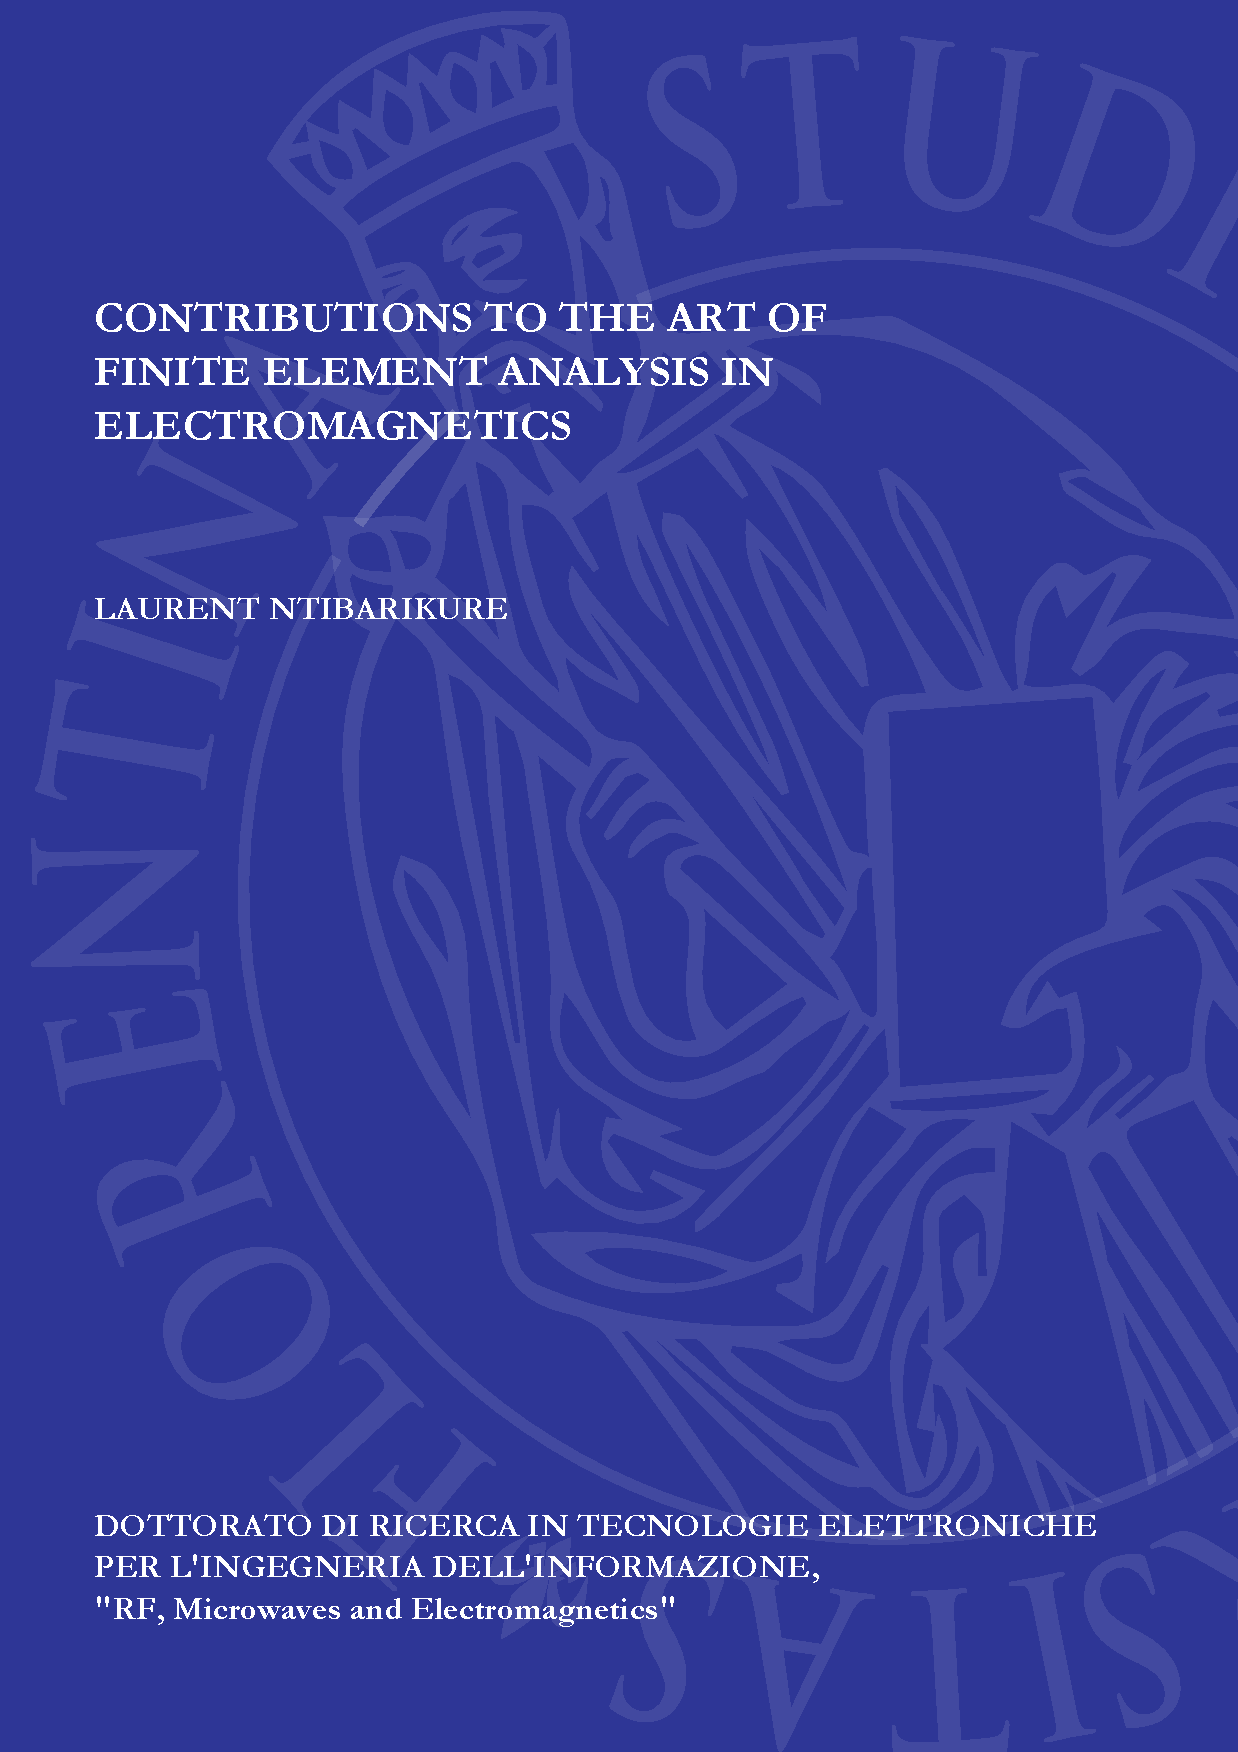
\includepdf[pages={1}]{cover/front.pdf}
\cleardoublepage
\graphicspath{{img/}}
\thispagestyle{empty}

\AddToShipoutPicture*{\AtPageCenter{\setlength\fboxsep{0pt}\makebox(0,0){
\includegraphics[width=0.9\paperwidth]{LOGOUNIFI_sfondo}}}}
\begin{figure}[h]
\centering

\includegraphics[width=6cm]{LOGOUNIFI}
\label{fig:UniFI}
\end{figure}
\begin{center} 
\vspace{1cm}
\Large{\textbf{\textsc{Dottorato di Ricerca}}}
\large{\textbf{\textsc{in}}\\[5pt]
\textbf{\textsc{Tecnologie Elettroniche per l'Ingegneria dell'Informazione\\[5pt]}}
%in\\[0pt]
}
\large{
\textsc{Indirizzo \quotes{\textit{RF, Microwaves and Electromagnetics}}}
\\[7pt]
\textsc{Ciclo} \ XXVI\\[45pt]
}
\textsc{\huge \textbf{Contributions~to~the~Art~of~\\\vspace{-5pt}Finite~Element~Analysis~in~\\\vspace{10pt} Electromagnetics}}\\[12pt]
\large{ING-INF/02}\\[20pt]
\Large{Laurent Ntibarikure}\\[25pt]
\end{center}
\vspace{30pt}
\noindent \textbf{Coordinatore:}\\[15pt]
\hspace*{20pt}	Prof. Gianfranco Manes\\[25pt]
\noindent \textbf{Tutori:}\\[15pt]
\hspace*{20pt}	Prof. Giuseppe Pelosi\\[15pt]
\hspace*{20pt}	Dr. Stefano Selleri\\[20pt]
\begin{center}
\large{2011-2013}
\end{center}

\newpage
\thispagestyle{empty}
\cleardoublepage
\thispagestyle{empty}
\par\vspace*{.35\textheight}{ 
\begin{flushright}\begin{minipage}{0.5\textwidth}
$\quad$ \textit{To Peter P. Silvester, whose teachings left in the nineties at the University of Florence have brought to me a deep interest on the matter.}
\end{minipage}\end{flushright}
}

\thispagestyle{empty}
\pagenumbering{roman}
% !TEX root = ln_diss.tex
\chapter*{Sommario}
Il metodo degli elementi finiti \`e un potente metodo per la soluzione di problemi  di valori al contorno complessi, governati da equazioni alle differenze parziali. La sua prima applicazione a problemi di ingegneria risale al 1943, anno in cui Courant divulg\`o la soluzione numerica di un problema di meccanica strutturale \cite{courant1943variational}. Da allora, vi sono stati numerosi tentativi di applicazione del metodo ad altri campi dell'ingegneria. Silvester, pioniere del metodo nel campo dell'elettromagnetismo applicato, nei suoi primi lavori datati 1969 %sulla rivista \quotes{Alta Frequenza} 
illustr\`o la possibilit\`a di risolvere problemi di guida d'onda con tale metodo \cite{silvester1969finite, coccioli1996finite}. Oggi giorno, vasto \`e il bagaglio di problemi elettromagnetici risolti e validati sperimentalmente. Molti ormai sono gli applicativi disponibili per l'analisi numerica agli elementi finiti di strutture guidanti e radianti.

Nonostante l'immenso sviluppo degli ultimi decenni, vi sono ancora molti problemi da risolvere. Nella presente tesi analizzeremo due di essi, fornendo alcune idee e tecniche risolutive. Il primo riguarda la soluzione di problemi \quotes{grandi}, irrisolubili con modesti comuni calcolatori, nel tentativo quindi di sfruttare al meglio le risorse computazionali disponibili ed oltrepassarne i limiti attuali. La strada della scomposizione di dominio \`e quindi stata impegnata. Suddividendo un  problema grande in vari sotto-problemi che per le loro dimensioni limitate risultano affrontabili singolarmente, e raccordando opportunamente le singole soluzioni \`e possible ottenere la soluzione del problema originale. Il secondo problema \`e legato all'imminente apparizione di materiali con caratteristiche elettromagnetiche intrinsecamente non lineari, ovvero dipendenti dal campo elettromagnetico in essi contenuto. L'analisi a microonde di tali mezzi con un approccio agli elementi finiti convenzionale non consente di raggiungere un sufficiente livello di accuratezza. L'analisi multiarmonica, includendo gli effetti non lineari, consente di migliorare notevolmente l'accuratezza di analisi. Un applicativo per l'analisi agli elementi finiti di problemi tridimensionali \`e stato implementato al fine di condurre le suddette ricerche.
\newpage
\thispagestyle{empty}
\cleardoublepage

\chapter*{Abstract}
The finite element method is a powerful method for the approximate solution of boundary value problems governed by partial differential equations. A really first application to structural engineering problems, dating 1943, is attributed to R. Courant \cite{courant1943variational}. Since then, there has been a lot of successful tentatives to apply the method to other fields. In particular, Silvester showed in 1969 \cite{silvester1969finite, coccioli1996finite} that waveguide modes could be easily computed with the method. His work started a long path for finite elements in electromagnetics, with multiple assessments of the method with real-world problems and gradually improving the efficiency of the algorithms. Nowadays, finite elements in computational electromagnetics has become an invaluable part in radio frequency and microwave application designs, and many packages are widely available to perform these tasks. 

However, there remain a lot of problems to be solved. In this dissertation, we have inquired in two of these. 
The first, the efficient solution of large problems which may not be solvable on a single modern computer. Domain decomposition methods have been thus investigated, these allowing to solve smaller parts of a large problem and to achieve the whole solution upon proper interconnection. Two types of domain decomposition methods have been analyzed, leading to the construction of algorithms for solving large electromagnetic problems at a nearly linear complexity. 
The other, the accurate solution of electromagnetic problems in which some materials behave nonlinearly, that is their properties vary depending on the intensity of the fields they imbue. Almost all materials behave nonlinearly and their effect is just a matter of fields intensities and accuracy requirements. In many microwave applications, the nonlinear effects, necessary for information processing and control, are still limited to lumped devices for their highly developed models. Accurate modeling of bulk or films of nonlinear materials may open the way to a new variety of controllable materials in flexible, reconfigurable, electromagnetic devices. A finite element package has been implemented to perform several tests here documented.

%Computers have also evolved during the last decades, increasing noticeably the computational power density up to the point a modern personal computer such as a low power laptop is several order more powerful than the first, room-sized, computers. Due to thermal power limitations, most of the modern processors are equipped with multiple cores, hence the algorithms are nowadays oriented to best exploit these architectures.

\vfill
\noindent \textit{Index Terms}: Electromagnetic radiation and scattering, time-harmonic fields, finite element method, domain decomposition methods, nonlinear materials, multiharmonic analysis, harmonic balance.
\thispagestyle{empty}
\cleardoublepage
% !TEX root = ln_diss.tex
\chapter*{Acknowledgements}

During these years of Ph.D. studies several persons (and I may forget many of them) have contributed to my work and without their support it would have been impossible for me to complete it. That is why I wish to dedicate this section to recognize their support.

I would like to express my sincere gratitude to the professors of my advisors: Prof. Giuseppe Pelosi and Dr. Stefano Selleri, for their guidance, motivation and support during this period.

I would like to acknowledge the financial support from Nuovo Pignone -- GE Oil and Gas, the research here presented being a part of my studies on electromagnetic compatibility modeling techniques.

Special thanks to all the employees, researchers and students of the Computational Electromagnetics laboratory of the Information Engineering department at the University of Florence, for their courtesy, the pieces of advice and help they gave me, and most of all for the good time spent together.

I would also like to express my appreciation to the pieces of knowledge also transferred to me all along my finite element methods for microwave engineering mastering quest by Prof. Romanus Dyczij-Edlinger, Prof. Jin Fa-Lee and Prof. Oszk\'ar B\'ir\'o. Deep appreciation also to Dr. Ortwin Farle, for many implementation skills imparted to me during my master thesis work at the \textit{Lehrstuhl f\"ur Theoretische Elektrotechnik} laboratory of Saarland University.

I would also like to express my heartfelt gratitude to my family for encouragement
and continuous support given throughout my life.

Last but not least, I would like to express my appreciation to my sweetheart, Veronica, for her love, patience, support and understanding throughout these difficult and challenging years.
\thispagestyle{empty}
\cleardoublepage
\setcounter{secnumdepth}{5}
\setcounter{tocdepth}{5}
\pdfbookmark[chapter]{\contentsname}{toc}
\tableofcontents
\newpage
\thispagestyle{empty}
\listoffigures
\newpage
\thispagestyle{empty}
\listoftables
\listofalgorithms
% !TEX root = ln_diss.tex
\chapter*{List of Publications}%\label{publications}
%\markboth{List of Publications}{}
%\addcontentsline{toc}{chapter}{List of Publications}
%\label{page:publications}
\section*{Refereed papers}
%\addcontentsline{toc}{section}{Refereed Journal Papers}
\begin{enumerate}[label={[\arabic*]}]
\item  L. Ntibarikure, G. Pelosi, S. Selleri, ``Efficient harmonic balance analysis of waveguide devices with nonlinear dielectrics,'' \emph{Microwave and Wireless Components Letters, IEEE}, vol. 22, no. 5, pp. 221--223, 2012.
\item  L. Ntibarikure, G. Pelosi, S. Selleri, ``Harmonic balance domain decomposition finite elements for nonlinear passive microwave devices analysis,'' \emph{Special Issue on \quotes{Finite Elements for Microwave Engineering}, Electromagnetics}, vol.~34, no. 3, 2014.
\end{enumerate}

\section*{Conference proceedings}
%\addcontentsline{toc}{section}{Refereed Journal Papers}
\begin{enumerate}[label={[\arabic*]}]
\item  L. Ntibarikure, ``Model order reduction in finite element analysis of phased array antennas,'' in \emph{Numero Speciale 8 - Serie di Elettromagnetismo su \quotes{XIX Riunione Nazionale di Elettromagnetismo (RiNEm)}, Atti della \quotes{Fondazione Giorgio Ronchi}}, vol. LXVIII, no. 4, pp. 97--102, 2012. [Barzilai award 2012]
\end{enumerate}


\section*{Conferences}
%\addcontentsline{toc}{section}{Refereed Conference Papers}
\begin{enumerate}[label={[\arabic*]}]
\item L. Ntibarikure, G. Pelosi, and S. Selleri, ``Harmonic balance domain decomposition finite element for nonlinear passive microwave devices analysis,'' in \emph{11th International Workshop on Finite Elements for Microwave Engineering -- FEM2012}, Estes Park, Colorado, USA, Jun. 4--6, 2012.
\item L. Ntibarikure, G. Pelosi, S. Selleri, ``Harmonic balance finite element analysis of third order intermodulation products in ferrite devices,'' in \emph{XIX Riunione Nazionale di Elettromagnetismo -- XIX~RiNEm}, Rome, Italy, Sep. 10--14, 2012.
\item  L. Ntibarikure, ``Model order reduction in finite element analysis of phased array antennas,'' in \emph{XIX Riunione Nazionale di Elettromagnetismo -- XIX~RiNEm}, Rome, Italy, Sep. 10-14, 2012.
\end{enumerate}

\thispagestyle{empty}
\cleardoublepage

\pagenumbering{arabic}
% !TEX root = ln_diss.tex
\chapter{Introduction} \label{chap:INT}

Nowadays, several successful commercial packages for solving electromagnetic problems are available. Such computational electromagnetics software is typically based on one or more \quotes{traditional} rigorous (full-wave) techniques such as the finite differences time-domain \cite{CSTMWS, SEMCADX} and the finite element method \cite{ComsolRF, HFSS}, which are differential based methods, or the method of moments \cite{FEKO} which is integral based, and sometimes include some of their hybridizations \cite{Garg2008, Davidson2011, RIB2011}. The robust formulations they implement have been validated throughout decades by multiple physical measurements of real-life applications, up to the point they form an invaluable part of current radio frequency and microwave engineering practice. Without these computational modeling methods, probably many highly technological applications would not have been realized yet.

However, many challenging applications still remain to be tackled due to the limited availability of computational resources. The higher is the electrical size of the problem, even if quite geometrically simple, the higher becomes the number of unknowns required to compute the fields and other related parameters. Some of these are large antenna arrays, antenna platform positioning problems, radar cross section of electrically large targets and with composite materials, terahertz and optical devices. The problem size, in terms of unknowns $N$ necessary for an acceptable (error controlled) analysis at a frequency $f$, typically scales as $N \propto O(f^3)$ for differential based methods and as $N \propto O(f^2)$ for integral methods \cite{lee2011maturity}. The same behavior is encountered for geometrically complicated models. Even if smaller than the wavelength, better accuracy is needed around the conductors corners and at interfaces between materials, some of the known sources of field singularities. Some of these applications are the frequency selective surfaces used as electromagnetic coatings and the signal integrity computation in high frequency integrated circuits \cite{lee2011maturity, mittra2004look}. A combination of geometrical and electromagnetic size complexities can be found in recent nano-optical applications, frequencies at which metals behave as high permittivity materials due to surface plasmons surrounded by the unitary permittivity of the air \cite{tsukerman2008computational}. Accurate solution of these kind of problems is still an active research field \cite{tsukerman1998comparison}.

Among all the problems that still remain to be solved, those comprehending nonlinear materials are still currently faced by the computational electromagnetics community, principally by the use of finite differences time-domain schemes which allow for straightforward implementation of nonlinearities \cite{goorjian1992direct, ziolkowski1993full, ziolkowski1994nonlinear, joseph1997fdtd, teixeira2008time, sasanpour2010analysis, potravkin2012numerical, frances2013split}. The main investigated fields of application initially were at optical frequencies, including harmonic generation, nano-plasmonics and solitons propagation in Kerr-like media. In fact, very high intensity fields are typically generated at those frequencies by lasers or even light emitting diodes, and hence materials that at microwave frequencies may behave as linear cannot anymore be accurately handled at optical ones with linear solvers. At lower frequencies, for the solution magneto-quasi-static problems like the evaluation eddy currents in ferromagnetic materials, a method using finite elements was early introduced by Silvester in 1970 \cite{silvester1970finite}. A time-harmonic scheme was there presented, allowing for fast computation of steady state fields. However, information on the distortion introduced by permeability saturation was still neglected. Years later, Yamada et al. \cite{yamada1988harmonic, yamada1989harmonic, yamada1991calculation} introduced a first multi-harmonic scheme, the harmonic balance finite element method, allowing for accurate treatment of nonlinearities \cite{gyselinck2002harmonic, pascal2003coupling, zhao2010analysis, zhao2011analysis}. Contemporaneously, finite element time domain schemes where introduced to allow transient analyzes \cite{biro1995various}. However, due to the immediate extrapolation of steady state fields which indeed are almost always sought for, a frequency-domain scheme often results to be preferable. It still appears that no multi-harmonic schemes have been employed from microwaves to optical frequencies.


\section{Efficient solvers for computational electromagnetics}

Even if they perform worse in terms of electrical size, differential based methods, leading to sparse matrices, can be directly solved with an asymptotic complexity of $O(N^2)$ \cite{gupta1997design} while the dense matrices of integral methods can be directly inverted with $O(N^3)$ complexity \cite{Cormen2009}. Furthermore, linear solvers (either stationary or not) behave dramatically worse as $N$ grows, thus require a particular attention to preconditioning in order to restore their performances. Three main approaches have been successfully adopted to steer the computational complexities of electromagnetic solvers down to linear or $O(N\log N)$:
\begin{itemize}
\item \textit{Multigrid methods}, which to some extent are based on multiple superimposed discretization levels, where the information derived from a coarse level (where a direct solver performs better) can be used to accelerate the computations on a finer level with a linear solver. This hierarchical decomposition of accuracy levels have been successfully employed for differential based methods \cite{Briggs2000, hill2003stabilized, ingelstrom2004higher, gheorghe2005multigrid, zhu2006multigrid, hill2006schnelle, ingelstrom2007comparison}. The integral based multigrid methods, referred as \quotes{multiresolution methods} \cite{vipiana2005multiresolution, khorrami2010fast}, are not yet affirmed as their differential counterparts.
\item \textit{Domain decomposition methods}, which follows the \textit{divide et impera} strategy, dividing a wide fine grid into smaller parts where the field solutions can be easily computed, then proper transmission conditions or subdomains coupling strategy have to be enforced in order to recover the fields within the whole domain \cite{quarteroni1999domain, toselli2005domain, mathew2008domain} . These methods have been extensively studied and employed to solve Maxwell's equations \cite{li2006vector, sun2005nonconforming, vouvakis2007domain, rodriguez2006new, zhao2006solving, barka2007domain, zhao2008domain, rawat2008domain, grasedyck2009domain, rawat2009finite, ozgun2010iterative, peng2010non, takei2010full, peng2011integral, shao2011full, wang2012domain,widlund2007domain} for both differential and integral methods (or their hybridization) up to tens of millions of unknowns with common personal computers.
\item \textit{Multipole methods}, which fundamentally group local method of moments near field solutions into multipoles that allow to compute far field couplings between the groups. These methods are intrinsically related to integral based methods, where dipole or multipoles can be accurately handled. They are known as the \textit{fast multipole method} or \textit{multilevel fast multipole algorithm} \cite{Chew2001, Gumerov2004} for integral equations.
\end{itemize}
In many cases, several difficulties remain for all the aforementioned methods. Typically based on some precise assumptions for which the iterative solvers they employ should converge, the end-user of the method still have to be highly skilled and experienced in order to properly conduct the analyzes. A lot of efforts still have to be done in order to achieve robust solvers, especially from the mathematics behind the implemented code.

Also, several improvements have been achieved to perform fast parameter sweeps. Once some solutions, for some parameter values, are computed by one of the previous \quotes{traditional} or efficient methods, fast intermediate solutions can be obtained by proper interpolation schemes. These are known as the \textit{model order reduction} methods \cite{farle2006multivariate, ntibarikure2012model} for differential based methods or as the \textit{characteristic basis functions} methods \cite{prakash2003characteristic} for integral based methods. Several parameter dependent solutions of full-wave methods are collected and orthonormalized with some spectral decomposition (Gram-Schmidt) or singular value decomposition. These solution vectors are then used to expand large-scale solutions on which the orginal problem is projected. Finally, if these solutions constitute a basis for the whole function space, then a few operations are sufficient to perform a parameter sweep with a controlled order of accuracy. The parameters can be the frequency of analysis, material properties, complex excitation amplitudes of a multiport device and many others. In principle, the large cost of multiple solutions computation in a parameter sweep is truncated once a good basis is found.

Among the \quotes{traditional} methods, differential based methods allow a straightforward treatment of materials properties and, for the finite element method, a better discretization of geometrical bodies. Integral methods are better suited for open problems, where the differential based methods require approximative boundary truncation techniques to implement Sommerfeld's radiation condition: absorbing boundary condtions \cite{Bayliss1982, Silvester1988} or perfectly matched layers (PMLs) \cite{Berenger1994}. However, many successful hybridizations of differential based and integral based methods have been reported \cite{xu1997hybrid, zhao2011efficient}. It is worth noticing that the introduction of integral equations has a significant drawback in reducing the computational efficiency \cite{zhao2006solving}. This has led to the choice of the finite element method as core development for efficient schemes that will be analyzed throughout this dissertation.

\section{A reason for nonlinear analyzes at microwaves}

It is well known that polycrystalline magnetic oxides like ferrites or other ferromagnetic compounds such the yttrium iron garnet, for their anisotropy, can be used to realize non-reciprocal microwave devices such as circulators, isolators and phase shifters \cite{pozar1998microwave, adam2002ferrite}. It is also known that these devices are typically critical when dealing with high power electromagnetic fields, due to the spurious fields they induce \cite{suhl1956nonlinear, suhl1957theory, bailey1979study}. Ferromagnetic materials were probably the first to present a nonlinear behavior at microwave frequencies. Very few attempts to predict the spurious fields generated in such devices have been reported in literature \cite{wu1976study, how1997nonlinear}.

Known as \textit{passive intermodulation}, the nonlinearities cause a critical limit in the design of microwave systems \cite{sanford1993passive} and their calculation methods are still very limited. This phenomenon is also imparted to metal contacts \cite{arazm1980nonlinearities}, metallic wires and dielectric cables \cite{amin1978coaxial} and particularly to metals oxidation \cite{bond1979intermodulation}. In a general form, these can be viewed as nonlinear electromagnetic properties of materials, that is field dependent permittivities, permeabilities and conductivities.

Also, during the last two decades, due to several improvements in the field of digital electronics, when seeking for thin-films materials with high permittivities to implement the capacitances in dynamic random access memories \cite{scott1994dielectric, shaw1999effect}, barium strontium titanate compounds have demonstrated a noticeable nonlinear behavior at microwave frequencies \cite{kozyrev1997ferroelectric, mateu2006measurements, mateu2007frequency, giere2007characterization}. Their electro-optic effect \cite{takeda2010dielectric}, principally due to a second order or Kerr-like permittivity, can hence be exploited to design tunable capacitors \cite{sigman2008voltage}, or in general to control the characteristics of any microwave device that use this kind of materials.

Finite elements can considerably help in the computation of nonlinear phenomena products, especially for its capability to easily handle material properties and geometries. Once again, it is the best suited computational electromagnetic method for nonlinear analyzes.

\section{Contributions of this dissertation}

The chosen fields of research have led to the implementation of a finite element software, namely \quotes{FES}. Several formulations have been implemented in FES, basically based on the application of the Galerkin framework on both two- and three-dimensional domains. The two-dimensional package, FES-2D, mainly coded in the high level Matlab$^\text{\circledR}$~language, was prevalently used to assess the formulations, which might result to be excessively time demanding to implement in lower level of abstraction languages. Then, the transfer of the formulations to tree-dimensional problems in FES-3D could be done relatively faster in an objective paradigm C++ code. FES-3D, using several third party, open source\footnote{Almost all the employed third party codes are at least provided with the in the Lesser General Public Licence, and some where totally free for reuse.}, codes, some written in Fortran or C, has been compiled with the GNU GCC 4.8.1 on {x86}\textunderscore{64} architectures with the -Ofast optimization flag enabled.

The present dissertation is structured as follows:
\begin{itemize}
\item The second chapter introduces to the electromagnetic radiation mechanism, which is known since more than a century to be governed by a set of partial differential equations collected into Maxwell's equations. A wave equation for the electric field is then derived, allowing for single partial differential equation solution. It is well known that this equation can be accurately solved by numerical methods as long as the frequency of analysis is above the lower limit that causes badly conditioned matrices, which is the case for all the experiments conducted here. The Galerkin framework is then introduced, with the necessary mathematical background to understand its efficacy. Finally, the formulations employed to solve, later on, several waveguide and radiation problems are introduced. Within this phase, the FES results are compared to commercial models analyzes for validation purposes.
\item In the third chapter, the domain decomposition concept is introduced with two different schemes, the Schur complement and the finite element tearing and interconnecting. Both the methods are tested on the simple case of a rectangular waveguide. Preconditioners for Krylov subspace methods are then built on a domain decomposition scheme and the convergence behavior is analyzed extensively. Finally, the numerical complexity of the method is derived to ensure its applicability to very large problems.
%a large frequency selective radome-enclosed patch antennas array is analyzed, showing the capabilities of the methods. 
\item In the fourth chapter, the first known attempt to apply the harmonic balance finite element method to microwave problems is presented. Almost all passive nonlinear problems require steady state computations and hence the method results to be very well suited. Several test cases on two-dimensional problems are shown to explain the method. One of the previous domain decomposition schemes have also been employed to accelerate the nonlinear analyzes. A three-dimensional barium strontium titanate based test case is shown, somehow proving the capabilities of the method.
\item Finally, some conclusions will be drawn in the last chapter. The analyzed and implemented methods open the way to many, still unperformed, analyzes. A possible outlook, matter of emerging technologies, will be hence discussed.
\end{itemize}


\thispagestyle{empty}
\cleardoublepage
% !TEX root = ln_diss.tex
\graphicspath{{img/ch1/}}
\chapter{Finite elements for the wave equation} \label{chap:FE}

\par This chapter introduces the boundary value problem that describes the radiation mechanism in an unbounded medium. The vector wave equation is then derived from Maxwell's eqations, being the partial differential equation that describes waves propagation. The finite element formulation for the electric field wave equation follows, presented for a full-wave solution of electromagnetic radiation problems. Several boundary conditions, that will be used throughout this dissertation, will be introduced here, allowing for the treatment of fields propagation analysis from either waveguides ports or free-space impinging waves. Some test cases will be shown, comparing to a commercial package, analyzing the FES implemented formulations behavior. FES is the core of the domain decomposition and the nonlinear analyzes presented, respectively, in chapters \ref{chap:DD} and \ref{chap:NL}.

%%%%%%%%%%%%%%%%%%%%%%

\section{Radiation in an unbounded medium}

\par The problem of electromagnetic radiation from a generic distribution of current sources in a unbounded medium relies on the solution of the Maxwell's equations \cite{rothwell2009electromagnetics}
\begin{eqnarray}
\nabla \times \mathcalb{E}(\mathbf{r},t) &= & -\frac{\partial}{\partial t}\mathcalb{B}(\mathbf{r},t) \qquad \qquad \qquad \quad \mathit{Faraday}\textrm{'}\mathit{\!s \ law}, \label{eq:tfaraday}  \\
\nabla \times \mathcalb{H}(\mathbf{r},t) &= & \frac{\partial}{\partial t}\mathcalb{D}(\mathbf{r},t) + \mathcalb{J}(\mathbf{r},t)  \quad \ \ \textit{Maxwell-Amp\`{e}re}\textrm{'}\mathit{\!s \ law}, \label{eq:tampere} \\[5pt]
\nabla \cdot \mathcalb{D}(\mathbf{r},t) &= & {\varrho}(\mathbf{r},t) \qquad \qquad \qquad \qquad \  \mathit{Poisson}\textrm{'}\mathit{\!s \ equation}, \label{eq:tpoisson}\\[5pt]
\nabla \cdot \mathcalb{B}(\mathbf{r},t) &= & 0 \qquad \qquad \qquad \qquad 	\ \ \ \ \mathit{Gauss}\textrm{'}\mathit{\! \ law \ for \ magnetism}, \label{eq:tgauss}
\end{eqnarray} where $\mathcalb{E}$ is the \textit{electric field intensity}, which carries the S.I.\footnote{Syst\`eme International d'unit\'es.} units $\mathrm{\nicefrac{\mathrm V}{\mathrm m}}$, $\mathcalb{H}$ the \textit{magnetic field intensity} in $\mathrm{\nicefrac{\mathrm A}{\mathrm m}}$, $\mathcalb{D}$ the \textit{electric displacement} in $\mathrm{\nicefrac{\mathrm C}{m^2}}$ (or $\mathrm{\nicefrac{\mathrm{As}}{m^3}}$), $\mathcalb{B}$ the \textit{magnetic induction} in $\mathrm{\nicefrac{\mathrm{Wb}}{m^2}}$ (or $\mathrm{\nicefrac{\mathrm{Vs}}{m^2}}$), $\mathcalb{J}$ the \textit{electric current density} in $\mathrm{\nicefrac{\mathrm A}{\mathrm m}}$ and $\mathcal{\varrho}$ the \textit{electric charge density} in $\mathrm{\nicefrac{\mathrm C}{m^3}}$ (or $\mathrm{\nicefrac{\mathrm{As}}{m^3}}$).
 All these values are dependent on the position vector $\mathbf{r} \in \mathbb{R}^3$ and on the time variable $t \in \mathbb{R}$. Combining the divergence of \eqref{eq:tampere} with \eqref{eq:tpoisson}, we obtain the \textit{current continuity equation}
\begin{equation}
\nabla \cdot \mathcalb{J}(\mathbf{r},t) + \frac{\partial}{\partial t} \mathcal{\varrho}(\mathbf{r},t) = 0.
\end{equation}
\par In order to solve Maxwell's system of first order partial differential equations (PDEs), it is necessary to provide the \textit{boundary conditions} and the \textit{initial conditions}. Furthermore, as the number of equations is less than the number of unknowns, we need to supply the \textit{constitutive relations}, which relates the electric displacement and the magnetic induction to the fields
\begin{eqnarray}
\label{eq:constgen1}
\mathcalb{D}(\mathbf{r},t) &= & \dyad{\epsilon}(\mathbf{r},t) \cdot \mathcalb{E}(\mathbf{r},t) \\
\label{eq:constgen2}
\mathcalb{B}(\mathbf{r},t) &= &  \dyad{\mu}(\mathbf{r},t) \cdot \mathcalb{H}(\mathbf{r},t),
\end{eqnarray} 
where $\dyad{\epsilon}$ and $\dyad{\mu}$ are dyadic tensors depending on the material in which the fields exist\footnote{The constitutive relations in (\ref{eq:constgen1}-\ref{eq:constgen2}) are stated in a form such that they can represent \textit{isotropic} and \textit{anisotropic} media.}. Also, in presence of conductive materials, the electric field gives birth to an electric current density
\begin{eqnarray}
\mathcalb{J}^c(\mathbf{r},t) &= &\dyad{\sigma}(\mathbf{r},t) \cdot \mathcalb{E}(\mathbf{r},t) \qquad \mathit{Ohm}\textrm{'}\mathit{\!s \ law},
\end{eqnarray}
where $\dyad{\sigma}$ is the \textit{electric conductivity} dyadic tensor in $\mathrm{\nicefrac{\mathrm S}{\mathrm m}}$, and the superscript \textit{c} on $\mathcalb{J}^c(\mathbf{r},t)$ indicates that the current density is induced by the electric field. With this additional equation, the current $\mathcalb{J}(\mathbf{r},t)$ in \eqref{eq:tampere} can be considered to be composed by an induced part, $\mathcalb{J}^c(\mathbf{r},t)$, and by an impressed part, $\mathcalb{J}^i(\mathbf{r},t)$, the latter actually being the source generating the electromagnetic fields.
%For a unbounded medium, the boundary conditions are those that ensure the fields extinction out of the domain investigated. This is possible by forcing the 
\par The boundary conditions ensure the continuity of the fields at the interfaces between different media, and this is stated as\footnote{The continuity equations (\ref{eq:conte1}-\ref{eq:contb1}) are derived from an integral solution of the Maxwell's equations, assuming a connected volume made by a part of region 1 and a part of region 2, i.e. a closed surface crossing the boundary interface between the two regions.}, for a surface interfacing two media,
\begin{eqnarray}
\hat{\mathbf{n}} \times \left ( \mathcalb{E}_1(\mathbf{r},t)-\mathcalb{E}_2(\mathbf{r},t) \right ) &= & 0,  \label{eq:conte1} \\
\hat{\mathbf{n}} \times \left ( \mathcalb{H}_1(\mathbf{r},t)-\mathcalb{H}_2(\mathbf{r},t) \right ) &= & \mathcalb{J}_s(\mathbf{r},t), \\
\hat{\mathbf{n}} \cdot \left ( \mathcalb{D}_1(\mathbf{r},t)-\mathcalb{D}_2(\mathbf{r},t) \right ) &= & \varrho_s(\mathbf{r},t), \\
\hat{\mathbf{n}} \cdot \left ( \mathcalb{B}_1(\mathbf{r},t)-\mathcalb{B}_2(\mathbf{r},t) \right ) &= & 0, \label{eq:contb1}
\end{eqnarray}
where $\hat{\mathbf{n}}$ is the unit vector normal to the surface, outwardly directed from the first region. $\mathcalb{J}_s$ and $\rho_s$ are the \textit{electric surface current density} in $\mathrm{\nicefrac{\mathrm A}{\mathrm m}}$ and \textit{electric surface charge density} in $\mathrm{\nicefrac{\mathrm C}{m^2}}$. %By (\ref{eq:conte1}-\ref{eq:contb1}), we obtain surface current and charge densities that keep informations on the fields outside (region 2) of the region in which the Maxwell's equations are solved (region 1), as if the whole domain were ununbounded.

\par For the radiation problem we need to solve in this chapter, we will consider \textit{isotropic} (\textit{homogeneous}) and \textit{time-invariant} media, for which the dyadics relating the fields to the electric displacement and magnetic induction are scalar values (diagonal tensors with equal entries). Thus, the constitutive relations become
\begin{eqnarray} 
\mathcalb{D}(\mathbf{r},t) &= \ \ \ \epsilon \mathcalb{E}(\mathbf{r},t) &= \ \ \ \epsilon_0 \epsilon_r \mathcalb{E}(\mathbf{r},t),  \label{eq:fsconst1}\\
\mathcalb{B}(\mathbf{r},t) &= \ \ \ \mu \mathcalb{H}(\mathbf{r},t)  &= \ \ \ \mu_0 \mu_r \mathcalb{H}(\mathbf{r},t), \label{eq:fsconst2}
\end{eqnarray}
where the constant $\epsilon_0 = 8.854 \times 10^{-12} \ \mathrm{\nicefrac{\mathrm F}{\mathrm m}}$ is the \textit{free-space permittivity}, $\epsilon_r$ the \textit{relative permittivity}, a non-dimensional constant, $\mu_0 = 4\pi \times 10^{-7} \ \mathrm{\nicefrac{\mathrm H}{\mathrm m}}$ is the \textit{free-space permeability} and $\mu_r$ the \textit{relative permeability}, also non-dimensional. As we expect electromagnetic waves to be propagating, we denote their speed as  $c = \nicefrac{1}{\sqrt{\epsilon \mu}} = \nicefrac{c_0}{\sqrt{\epsilon_r \mu_r}}$ with $c_0  \approx 2.998 \times 10^{8} \ \mathrm{\nicefrac{\mathrm m}{s}}$ the \textit{free-space speed of light}.

\par For the solution of Maxwell's equations, there must be also given the initial conditions, that is, the values of the sources and the fields on the boundaries at the initial observation time $t=t_0$. Our treatment will consider the frequency-domain formulation of the fields invoking the spectral representation of time dependent fields by the \textit{Fourier integral theorem}  $${\psi}(\mathbf{r},t) = \frac{1}{2\pi} \int_{-\infty}^{\infty} {\Psi} (\mathbf{r}, \omega) \mathrm{e}^{j\omega t} d\omega.$$ Applying the \textit{Fourier integral theorem} to the Maxwell's equations (\ref{eq:tfaraday}-\ref{eq:tgauss}), we obtain
\begin{eqnarray}
\nabla \times {\mathbf{E}}(\mathbf{r},\omega) &= & -j\omega{\mathbf{B}}(\mathbf{r},\omega), \label{eq:ffaraday} \\
\nabla \times {\mathbf{H}}(\mathbf{r},\omega) &= & j\omega{\mathbf{D}}(\mathbf{r},\omega) + {\mathbf{J}}(\mathbf{r},\omega), \label{eq:fampere} \\
\nabla \cdot {\mathbf{D}}(\mathbf{r},\omega) &= & {\rho}(\mathbf{r},\omega), \label{eq:fpoisson}\\
\nabla \cdot {\mathbf{B}}(\mathbf{r},\omega) &= & 0,\label{eq:fgauss}
\end{eqnarray}
and to the continuity equation we obtain
\begin{equation}
\nabla \cdot {\mathbf{J}}(\mathbf{r},\omega) + j \omega {\rho}(\mathbf{r},\omega) = 0, \label{eq:contJ}
\end{equation}
where we have used the Fourier integral of the time derivatives operator $$\frac{\partial}{\partial{t}}{\psi}(\mathbf{r},t) \leftrightarrow j\omega {\Psi} (\mathbf{r}, \omega),$$
$\omega$ being the angular frequency ($\omega = 2 \pi f$ with $f$ the frequency in $\mathrm{Hz}$) and $j = \sqrt{-1}$. The frequency dependent function ${\Psi}(\mathbf{r},\omega)$ represents the spectrum of the time dependent function ${\psi}(\mathbf{r},t)$, obtained by the \textit{Fourier Transform} $${\Psi} (\mathbf{r}, \omega) = \int_{-\infty}^{\infty} {\psi}(\mathbf{r},t) \mathrm{e}^{-j\omega t} dt \qquad \in \mathbb{C}, \ \forall \omega \in \mathbb{R}.$$ 
The spectral formulation allows us to neglect the initial conditions, the spectrum being computed by an integral over the entire domain of $t$ ($t \in \mathbb{R}$).
Also, with the spectral representation, the constitutive relations in isotropic media become
\begin{eqnarray} 
{\mathbf{D}}(\mathbf{r},\omega) &= & \epsilon_0 \epsilon_r {\mathbf{E}}(\mathbf{r},\omega),  \label{eq:ffsconst1}\\
{\mathbf{B}}(\mathbf{r},\omega) &= & \mu_0 \mu_r {\mathbf{H}}(\mathbf{r},\omega). \label{eq:ffsconst2}
\end{eqnarray}


\section{The time harmonic wave equation} %%%%%%%%%%%%%% WAVE EQUATION

\par The solutions ${\mathbf{E}}(\mathbf{r},\omega)$ and ${\mathbf{H}}(\mathbf{r},\omega)$ of the Maxwell equations (\ref{eq:ffaraday}-\ref{eq:fgauss}), can be computed using the \textit{frequency-domain wave equation} in the electric field, obtained combining the curl of Faraday's equation \eqref{eq:ffaraday} and the constitutive relation \eqref{eq:ffsconst2},
\begin{eqnarray}
\nabla \times \frac{1}{\mu_r} \nabla \times {\mathbf{E}}(\mathbf{r},\omega) &= & - j\omega\mu_0 \nabla \times {\mathbf{H}}(\mathbf{r},\omega), 
\end{eqnarray}
\noindent then, by the use of Maxwell-Amp\`ere's law \eqref{eq:fampere} and the constitutive relation \eqref{eq:ffsconst1}, we obtain
\begin{eqnarray}
\nabla \times \frac{1}{\mu_r} \nabla \times {\mathbf{E}}(\mathbf{r},\omega) - k_0^2 \epsilon_r {\mathbf{E}}(\mathbf{r},\omega) &= & - jk_0\zeta_0{\mathbf{J}}(\mathbf{r},\omega),  \label{eq:waveE}
\end{eqnarray}
where $k_0 = \omega \sqrt{\epsilon_0 \mu_0} = \nicefrac{\omega}{c_0} = \nicefrac{2\pi}{\lambda_0}$ is the \textit{free space wavenumber} in $\frac{1}{\mathrm{m}}$, with $\lambda_0$ the \textit{free space wavelength} in meters, and $\zeta_0 = \omega \sqrt{\frac{\mu_0}{\epsilon_0}}$ is the \textit{free space impedance} in $\mathrm{\Omega}$\footnote{One can straightforwardly deduce that the scalar term $\omega \mu_0$ that scales the current density is equivalent to $k_0 \zeta_0$.}. The solutions of these second-order PDEs are the same as the ones of the first-order Maxwell's PDEs, as long as the fields are spatially twice differentiable everywhere. As we will see later, this complication will be removed with the introduction of the weak form employed in the finite elements formulation.

Throughout this dissertation, we will analyze bounded media. Due to computational resources limitations, the real-world domain is restricted to the parts where the fields are to be computed, encompassing the device or object to analyze. As we will see later, proper boundary conditions will be used to enforce continuity of the fields from the domain to the surrounding and \textit{viceversa}. Furthermore, we will consider the computational domain devoid of electromagnetic fields sources, hence ${\mathbf{J}^i}(\mathbf{r},\omega)$ can be drop in \eqref{eq:waveE}, keeping only the induced current densities ${\mathbf{J}^c}(\mathbf{r},\omega)$. Also, we will consider the electric field to have a \textit{time-harmonic} dependence (and so will have the magnetic field) of the form
\begin{eqnarray}
\mathcalb{E}(\mathbf{r},t) =  \mathfrak{Re} \left( \tilde{\mathcalb{E}}(\mathbf{r}) \ \exp{j\omega t} \right) &\leftrightarrow &{\mathbf{E}(\mathbf{r})}. \label{eq:waveHarmE}
\end{eqnarray}
\noindent Only one frequency will be treated at a time where material properties behave linearly (independent form the electromagnetic fields flowing through them), and in nonlinear analyzes (Chapter \ref{chap:NL}), materials will receive a special treatment in order to consider the higher-order harmonics generated, and their coupling behavior. As a result, the time-harmonic wave equation for the electric field can be written as
\begin{eqnarray}
\nabla \times \frac{1}{\mu_r} \nabla \times {\mathbf{E}} + j k_0 \zeta_0 \sigma {\mathbf{E}} - k_0^2 \epsilon_r {\mathbf{E}} &= & 0, \label{eq:waveeqE}
\end{eqnarray}
\noindent where, for the sake of simplicity, $\mathbf{r}$ have been drop. Once \eqref{eq:waveeqE} is solved for $\mathbf{E}$, the magnetic field $\mathbf{H}$ can be straightforwardly recovered with of the use of \eqref{eq:ffaraday}, together with the constitutive relations. For instance,
\begin{eqnarray}
{\mathbf{H}} &= & \frac{\nabla \times {\mathbf{E}}}{-j k_0\zeta_0\mu_r}.  \label{eq:waveeqErecH}
\end{eqnarray}

\section{Finite element method}

The principal peculiarity of the finite element method (FEM) is the division of a given domain $\Omega$ into a set of simple subdomains, called \textit{finite elements}. The underlying principle of the method is to replace the entire continuous domain with a number of interconnected finite elements, the so-called \textit{mesh} $\mathcal{M}_h(\Omega)$), in which the unknown function is approximated by a finite linear combination of simple basis functions or \textit{shape functions} with unknown coefficients. Then, the local system of algebraic relations, related to the PDE we wish to solve, is derived in each element upon applying either the Rayleigh-Ritz Method (variational procedure) or, most commonly, the Weighted Residual Method in the Galerkin framework. Finally, the local systems of equations computed for each element are assembled to obtain a global system of equations to solve for the unknown function over the whole domain $\Omega$. 

The main four steps of the FEM procedure can be summarized as follows:
\begin{itemize}
\setlength{\itemsep}{0pt}
\item \textit{Preprocessing}: define the computational domain $\Omega$ of the problem, select the domain truncation method (waveports truncation and radiation boundaries for electromagnetic problems) building a pertinent CAD (Computer Aided Design) model, select the types of finite elements and discretize the domain with finite elements to create the mesh $\mathcal{M}_h(\Omega)$,
\item \textit{Assembly}: after accurate evaluation of the function space of the problem to be solved, select the basis functions and their polynomial order. Then generate the element matrices by the application, over each element, of the Rayleigh-Ritz Method or the Weighted Residual Method to the PDE. The integral equation of the previous methods may allow, depending on the PDE, to obtain the weak variational form upon applying integration by parts. Assemble the local element matrices to form the global system of equations which will be sparse due to the compact supports of the basis funcions, and finally impose the boundary conditions,
\item \textit{Solution}: the resulting global system of equations, stated in a matrix form, can now be solved either with direct methods (Gaussian elimination optimized for sparse matrices, maybe after LU or Cholesky factorization) or iterative methods (stationary or Krylov subspace), with proper preconditioning (Incomplete LU or Cholesky, Successive Over Relaxation, Jacobi, Gauss-Seidel) of the system matrix,
\item \textit{Postprocessing}: retrieve the interpolated function to extract the parameters of interest (modal scattering parameters, radiation pattern, radar cross section or simply the fields for visualization).
\end{itemize}

\subsection{Mesh generation}

The mesh generation is perhaps the most important and difficult phase of the FEM procedure as it affects the computational requirements (both memory and CPU times), and the accuracy of the results. The shape of elements should provide the best conformity of the mesh to the CAD model, especially for complex geometries. Common element shapes (Fig. \ref{fig:Elements}) are triangles and quadrilaterals for 2D models, tetrahedra and hexahedra for 3D models \cite{cubit}. Triangles and tetrahedra are called simplices. A fundamental characteristic of simplices is that any polygon or polyhedron can be expressed as the union of simplices. This renders them the best suited to model curved surfaces and irregular regions (Fig. \ref{fig:Mesh}).

\begin{figure}[h!]
\centering
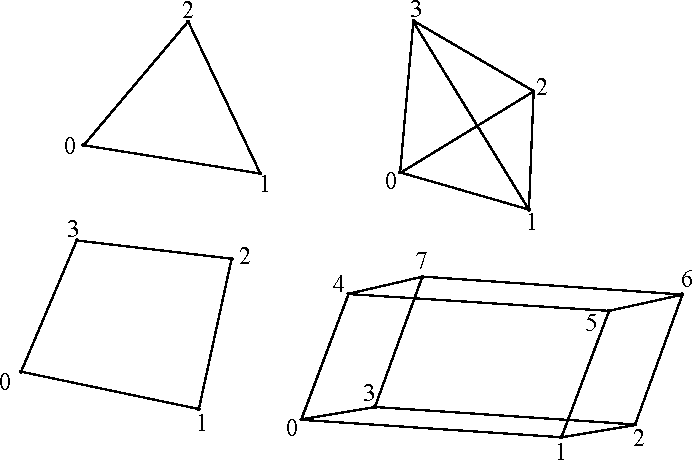
\includegraphics[width=10cm]{Elements}
\caption{Common element shapes. Left to right, top to bottom: triangle, tetrahedron, quadrilateral and hexahedron.}
\label{fig:Elements}
\end{figure}

\begin{figure}[h!]
\centering
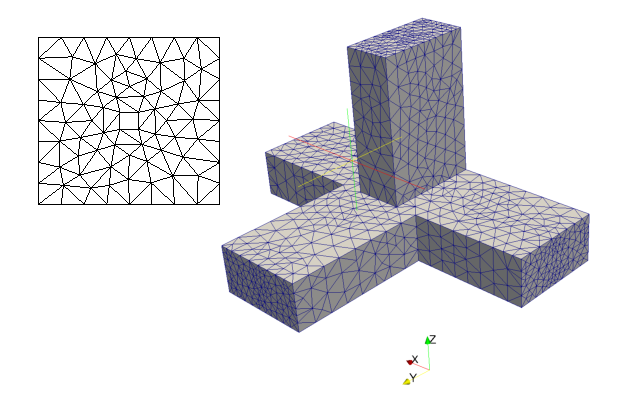
\includegraphics[width=12cm]{Mesh}
\caption{Finite element meshes. Left to right: triangularization a square domain surrounding a small square, tetrahedralization of microwave Magic-Tee.}
\label{fig:Mesh}
\end{figure}

As the mesh is used as the support for a piecewise linear approximation of a function, the accuracy of the approximation directly depends on the sizes and shapes of the elements. If the elements are small enough (typically less than $\frac{\lambda}{10}$ per side), then the field inside the element can be reliably approximated by linear polynomials. For greater dimensions, one may increase the polynomial order to achieve better approximation at the cost of an increase of the interpolation coefficients number.

The accuracy is also related to the elements shape and how far they are to be \quotes{regular} or equilateral: there is a mathematical connection between the mesh \quotes{quality}, the interpolation errors and the global matrix conditioning \cite{tsukerman1998comparison}. Low quality, \quotes{needle-like}, elements may increase the condition number of the system matrix (poor conditioning), and consequently, may cause a degradation in the accuracy of the results. There have been a lot of efforts in finding the best compromise between the generation of good quality mesh while containing the computational requirements. The most diffused approach is the adaptive mesh refinement ($h$-AMR), where appropriately chosen error indicators (mainly based on the gradient of the function) are used to refine locally higher error elements (next to metallic corners, discontinuities in material properties and any other potential singularity of the function) of the mesh \cite{sun2000adaptive,ingelstrom2004higher}. Other approaches are a combination of the elements refinements ($h$-refinements) and the polynomial orders refinements ($p$-refinements) which lead to a better compromise \cite{solin2010adaptive}.

FES package integrates, in the 2D form, the Triangle Mesh Generator \cite{shewchuk2002delaunay} and, in the 3D form, TetGen \cite{si2008three}. Both are based on the Delaunay triangulation which intrinsically allow for optimized mesh quality control, even for really complex geometries. Also, for validation purposes, meshes generated from commercial packages, Comsol (2D) and HFSS (3D), can be imported  in the analogous version of FES, restricting in such a way the errors to the steps of the finite element method following the mesh generation, mainly assembly and solve steps.


\subsection{Shape functions}

Accurate definition of the functional space of the solution is necessary to obtain physical solutions. In fact, the PDE with the necessary boundary conditions (initial conditions neglected for the time-harmonic assumption) treated until now, in a totally continuous space, are sufficient to prove existence and uniqueness of the solution. In a discretized world, this might not be true. However, one of the most important results of numerical solution of PDE is given by Cea's theorem \cite{ciarlet1978finite}, the equivalent functional analysis' Max-Milgram theorem, which in simple terms states that once one can prove that a linear operator (the PDE) on a specific functional space is bounded, then the numerical solution to the PDE exists and is unique within a bounded error (maximum error). Furthermore, as the finite discretization tends to the continuous case ($\mathcal{M}_h(\Omega) \rightarrow \Omega$), the error tends to vanish. This is the fundamental aspect of the finite elements: there is a convergence of the numerical solution to the exact solution. 

As a consequence, we need to provide the proper function spaces in which the operators for Maxwell's equations (curls, divergences, gradients) are bounded. We define the \quotes{boundedness} of the solution in $\Omega$ in terms of the Euclidean distance or, more generally, the Lebesgue space $\mathcal{L}^2(\Omega)$. Furthermore, we define the $D$-dimensional ($D := 2,3$) Lebesque space to be a Hilbert space in such a way that
$$\left (\mathcal{L}^2(\Omega)\right)^D = \left \lbrace \mathbf{v} : \Omega \rightarrow \mathbb{C}^D \ | \ \Vert \mathbf{v}\Vert_{(\mathcal{L}^2(\Omega))^D }  = \int_\Omega |\mathbf{v}|^2 d\Omega < \infty \right \rbrace.$$

To guarantee the boundedness of differential operators in vector spaces, we introduce some important Sobolev spaces \cite{monk2003finite}.

\subsubsection{\texorpdfstring{$\mathcal{H}^1(\Omega)$ Sobolev space}{H1 Sobolev space}}

One of the Sobolev spaces, related to all the square integrable functions that have square integrable gradient, is defined as

$$\mathcal{H}^1(\Omega) = \left \lbrace \phi \in \mathcal{L}^2(\Omega) \ | \ \nabla \phi \in (\mathcal{L}^2(\Omega))^D \right \rbrace,$$

\noindent with the norm

$$\Vert\phi\Vert_{\mathcal{H}^1(\Omega)} = \left( \Vert\phi\Vert_{\mathcal{L}^2(\Omega)}^2 + \Vert\nabla \phi\Vert_{(\mathcal{L}^2(\Omega))^D}^2 \right)^{1/2}.$$

\noindent As we will see, this is the \quotes{home} space for the electric field in 2D transversal magnetic formulation for the wave equation. This space and related formulations have been used extensively to assess the domain decomposition and nonlinear analyses of chapters \ref{chap:DD} and \ref{chap:NL}. More generally, this is the home for scalar potentials and for electric charge densities.

\subsubsection{\texorpdfstring{$\mathcal{H}(\mathrm{curl},\Omega)$ Sobolev space}{Hcurl Sobolev space}}

Another important Sobolev space, related to all the square integrable functions that have square integrable curl, is defined as
%
$$\mathcal{H}(\mathrm{curl},\Omega) = \left \lbrace \mathbf{v} \in (\mathcal{L}^2(\Omega))^D \ | \ \nabla  \times \mathbf{v} \in (\mathcal{L}^2(\Omega))^D \right\rbrace,$$
%
\noindent with the norm
%
$$\Vert\mathbf{v}\Vert_{\mathcal{H}(\mathrm{curl},\Omega)} = \left( \Vert \mathbf{v} \Vert_{(\mathcal{L}^2(\Omega))^D}^2 + \Vert\nabla \times \mathbf{v} \Vert_{(\mathcal{L}^2(\Omega))^D}^2 \right)^{1/2}.$$
%
\noindent This space fundamentally represents the electric and magnetic field intensities, $\mathbf{E}$ and $\mathbf{H}$, within Maxwell's equations.
%
\subsubsection{\texorpdfstring{$\mathcal{H}(\mathrm{div},\Omega)$ Sobolev space}{Hdiv Sobolev space}}
%
Another important Sobolev space, related to all the square integrable functions that have square integrable divergence, is defined as
%
$$\mathcal{H}(\mathrm{div},\Omega) = \left\lbrace \mathbf{v} \in (\mathcal{L}^2(\Omega))^D \ | \ \nabla  \cdot \mathbf{v} \in (\mathcal{L}^2(\Omega))^D \right\rbrace,$$
%
\noindent with the norm
%
$$\Vert\mathbf{v}\Vert_{\mathcal{H}(\mathrm{div},\Omega)} = \left( \Vert \mathbf{v} \Vert_{(\mathcal{L}^2(\Omega))^D}^2 + \Vert\nabla \cdot \mathbf{v} \Vert_{(\mathcal{L}^2(\Omega))^D}^2 \right)^{1/2}.$$
%
\noindent This space fundamentally represents the electric and magnetic inductions intensities, $\mathbf{D}$ and $\mathbf{B}$, and the electrical current density $\mathbf{J}$ within Maxwell's equations.
%
\subsubsection{de Rham complex}
%
Here comes an interesting result pertaining to the Sobolev spaces defined above: the vector identities $\nabla \times \nabla \phi = 0$ and $\nabla \cdot \nabla \times \mathbf{v} = 0$, where $\phi \in \mathcal{H}^1(\Omega)$ and $\mathbf{v} \in \mathcal{H}(\mathrm{curl},\Omega)$, can be used to establish a relationship between the spaces. For instance, in view of identity $\nabla \times \nabla \phi = 0$, $\nabla \phi \in \mathcal{H}(\mathrm{curl},\Omega)$ and $\nabla \cdot \nabla \times \mathbf{v} = 0$ implies $\nabla \times \mathbf{v} \in \mathcal{H}(\mathrm{div},\Omega)$. These relationships can be summarized as

$$\mathcal{H}^1(\Omega) \ \stackrel{\nabla}{  \longrightarrow} \ \mathcal{H}(\mathrm{curl},\Omega) \ \stackrel{ \nabla\times}{ \longrightarrow} \ \mathcal{H}(\mathrm{div},\Omega) \stackrel{\nabla\cdot}{ \longrightarrow} \ \mathcal{L}^2(\Omega),$$

\noindent and important mapping can be immediately visualized with this so-called de Rham complex: gradients map $\mathcal{H}^1(\Omega)$ to $\mathcal{H}(\mathrm{curl},\Omega)$ and curls map $\mathcal{H}(\mathrm{curl},\Omega)$ to $\mathcal{H}(\mathrm{div},\Omega)$. 

The electromagnetic quantities and their corresponding function space are shown in table \ref{tab:quantspace}.


\begin{table}[h!]
\begin{center}
\begin{tabular}{|c|c|}
\hline 
Quantity & Function space \\ 
\hline
\hline 
$\mathbf{E}, \mathbf{H}$ & $\mathcal{H}(\mathrm{curl},\Omega)$ \\ 
\hline 
$\mathbf{D}, \mathbf{B}, \mathbf{J}$ & $\mathcal{H}(\mathrm{div},\Omega)$ \\ 
\hline 
$\rho$ & $\mathcal{L}^2(\Omega)$ \\ 
\hline 
$\epsilon_0 \dyad{\epsilon}_r, \mu_0 \dyad{\mu}_r$ & $\mathcal{H}(\mathrm{curl},\Omega) \longrightarrow \mathcal{H}(\mathrm{div},\Omega)$ \\ 
\hline 
\end{tabular}
\end{center}
\caption{Electromagnetic quantities and their function space.}
\label{tab:quantspace}
\end{table}

\subsubsection{Scalar and rotational basis functions}

The basis functions chosen to expand the $\mathcal{H}^1(\Omega)$ space, especially tailored to expand scalar functions, are based on the simplex coordinates $\phi_i$ \cite{pelosi2009quick}. $\phi_i$ is the continuous function that is linear on each triangle or tetrahedron, being one at node $i$ and zero at all other nodes.

Each basis function is associated with either a node $\lbrace i \rbrace$, an edge $\lbrace ij \rbrace$, a triangular face $\lbrace ijk \rbrace$ or a tetrahedron $\lbrace ijkl \rbrace$ of the mesh.

The continuous, scalar ($\mathcal{H}^1(\Omega)$-conforming) finite element spaces of order $p$ are given by $\mathcal{V}^p = \mathcal{S}^1 \oplus \ldots \mathcal{S}^p$, where $\mathcal{S}^p \subset \mathcal{H}^1(\Omega)$ are given in table \ref{tab:H1functions}. We note that the functions in $\mathcal{V}^p$ are continuous across element boundaries.

\begin{table}[h!]
\begin{center}
\begin{tabular}{|c|c|c|}
\hline 
Space & Basis functions & Mesh entity \\ 
\hline
\hline 
$\mathcal{S}^1$ & $\phi_i$ & $\lbrace i \rbrace$ \\ 
\hline 
$\mathcal{S}^2$ & $\phi_i\phi_j$ & $\lbrace ij \rbrace$ \\ 
\hline 
$\mathcal{S}^3$ & $\phi_i\phi_j(\phi_i - \phi_j)$ & $\lbrace ij \rbrace$ \\ 
 & $\phi_i\phi_j\phi_k$ & $\lbrace ijk \rbrace$ \\ 
\hline 
\end{tabular} 
\end{center}
\caption{$\mathcal{H}^1(\Omega)$-conforming basis functions up to order $p = 3$.}
\label{tab:H1functions}
\end{table}


For the rotational basis functions, we have chosen to expand the $\mathcal{H}(\mathrm{curl},\Omega)$ with N\'ed\'elec incomplete order spaces \cite{nedelec1980mixed} which often lead to sparser matrices than the complete order counterpart while achieving approximately the same accuracy. They also permit the use of different elemental orders in a single finite element iterative solution with $p$-multilevel preconditioners \cite{sun2001construction}. The $\mathcal{H}(\mathrm{curl},\Omega)$-conforming finite element space of order $p$ is hence constructed recursively,

$$\mathcal{W}^p = \mathcal{W}^{p-1} \oplus \bar{\mathcal{W}}^{p} \ \mathrm{for} \ p = 2, 3 \ \mathrm{and} \ \mathcal{W}^{1}= \mathcal{R}^{1},$$

\noindent with the incremental space $\bar{\mathcal{W}}^p = \mathcal{R}^p \oplus \nabla \mathcal{S}^p$. The tangential components of $\mathcal{W}^p$ are continuous across element boundaries whereas the normal component may be discontinuous.

\begin{table}[h!]
\begin{center}
\begin{tabular}{|c|c|c|}
\hline 
Space & Basis functions & Mesh entity \\
\hline
\hline 
$\mathcal{R}^1$ & $\phi_i\nabla\phi_j-\phi_j\nabla\phi_j$ & $\lbrace ij \rbrace$ \\
\hline 
$\mathcal{R}^2$ & $3\phi_j\phi_k\nabla\phi_i-\nabla(\phi_i\phi_j\phi_k)$ & $\lbrace ijk \rbrace$ \\
 & $3\phi_k\phi_i\nabla\phi_j-\nabla(\phi_i\phi_j\phi_k)$ & $\lbrace ijk \rbrace$ \\
\hline 
$\mathcal{R}^3$ & $4\phi_j\phi_k(\phi_j - \phi_k)\nabla\phi_i - \nabla\left(\phi_i\phi_j\phi_k(\phi_j-\phi_k)\right)$ & $\lbrace ijk \rbrace$ \\
 & $4\phi_k\phi_i(\phi_k - \phi_i)\nabla\phi_j - \nabla\left(\phi_i\phi_j\phi_k(\phi_k-\phi_i)\right)$ & $\lbrace ijk \rbrace$ \\
 & $4\phi_i\phi_j(\phi_i - \phi_j)\nabla\phi_k - \nabla\left(\phi_i\phi_j\phi_k(\phi_i-\phi_j)\right)$ & $\lbrace ijk \rbrace$ \\
 & $4\phi_j\phi_k\phi_l\nabla\phi_i - \nabla(\phi_i\phi_j\phi_k\phi_l)$ & $\lbrace ijkl \rbrace$ \\ 
 & $4\phi_k\phi_l\phi_i\nabla\phi_j - \nabla(\phi_i\phi_j\phi_k\phi_l)$ & $\lbrace ijkl \rbrace$ \\ 
 & $4\phi_l\phi_i\phi_j\nabla\phi_k - \nabla(\phi_i\phi_j\phi_k\phi_l)$ & $\lbrace ijkl \rbrace$ \\ 
\hline 
\end{tabular} 
\end{center}
\caption{$\mathcal{H}(\mathrm{curl},\Omega)$-conforming basis functions up to order $p = 3$.}
\label{tab:Hcurlfunctions}
\end{table}

\subsection{Galerkin framework}

Among the finite element formulations, the Galerkin approach is the most straightforward to achieve finite element matrices. While the Rayleigh-Ritz approach requires to derive the proper Hamiltonian that describes the physics of the problem,  minimizing it, the Galerkin approach simply requires to define projections, which may be intrinsic from the definition of the shape functions in a Hilbert space. In fact, in a Hilbert space, the projection from a space to another is given by the Lebesgue scalar product 
%
$$<\mathbf{u},\mathbf{v}> = \int_\Omega \mathbf{u}^* \mathbf{v} \ d\Omega,$$
%
\noindent where $^*$ implies the adjoint operator (hermitian transpose). Furthermore, the original Galerkin projection is such that the space of origin $\mathcal{V}$ is the same of the arrival space $\mathcal{V}$. 

Consider the linear operator $A : \mathcal{V} \longrightarrow \mathcal{V}$, the corresponding homogeneous system is
$$A \mathbf{v} = \mathbf{f},$$
\noindent where $\mathbf{v} \in \mathcal{V}$ and $\mathbf{f} \in \mathcal{V}$. With the Galerkin approach, we seek $\mathbf{v} \in \mathcal{V}$ such that
$$< \mathbf{t}, A \mathbf{v}> = <\mathbf{t},\mathbf{f}>, \quad \forall \mathbf{t} \in \mathcal{V}.$$
\noindent Let us also assume the $N$-dimensional space $\mathcal{V}_h\in \mathcal{V}$ described by shape functions $\mathbf{v}_j$ such that $\mathbf{v}_h = \sum_{j=1}^N x_j \mathbf{v}_j$ and $\mathbf{t}_h = \mathrm{span}\lbrace{\mathbf{v}_1, \ldots, \mathbf{v}_i, \ldots, \mathbf{v}_n}\rbrace$. If we seek $\mathbf{v}_h \in \mathcal{V}_h$ such that
\begin{equation}
\sum_{i=1}^N x_j < \mathbf{v}_i, A \mathbf{v}_j> = <\mathbf{v}_i,\mathbf{f}>, \quad \forall \mathbf{v}_i, \ \ \ i=1,\ldots,N,
\label{eq:Galerkin}
\end{equation}
%
\noindent and, by Cae's theorem, $\mathbf{v}_h$ exists and is unique. The system \eqref{eq:Galerkin} can be turned into an $N$-dimensional set of linear equations whose solution is found by solving the $(N \times N)$-matrix system
$$ \mat{A} \ \vect{x} = \vect{b}.$$
The matrix entries $\mathrm{A}_{ij} = < \mathbf{v}_i, A \mathbf{v}_j>$, the source vector entries are $\mathrm{b}_i = <\mathbf{v}_i,\mathbf{f}>$ and the unknown $\vect{x}$ contains the expansion coefficients $x_j$ for the solution $\mathbf{v} \approx \mathbf{v}_h = \sum_{j=1}^N x_j \mathbf{v}_j$.


\subsubsection{Problem model}

Let us consider the domain $\Omega \subset \mathbb{R}^3$ to be bounded by $\mathrm{\partial \Omega = \Gamma = \Gamma_E \cup \Gamma_{H} \cup \Gamma_{WG} \cup \Gamma_R}$ for the antenna problem and by $\mathrm{\partial \Omega = \Gamma = \Gamma_E \cup \Gamma_{H} \cup \Gamma_R}$ for the scattering problem as depicted in figure \ref{fig:FEMproblem}.
\begin{figure}[hbpt!]
\centering
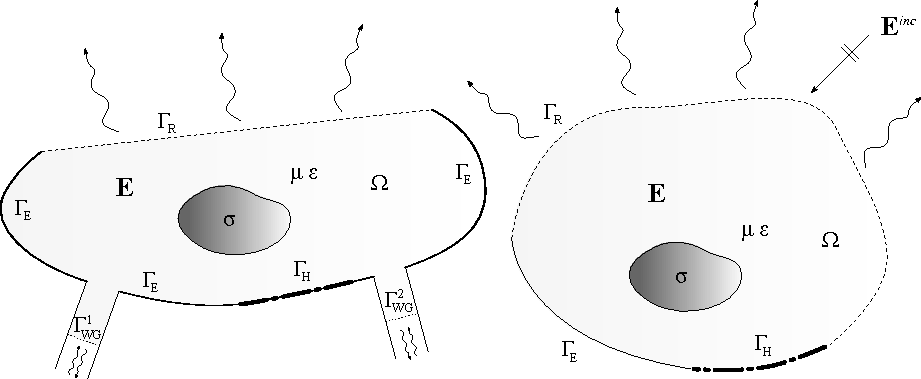
\includegraphics[width=12cm]{FEMproblem} 
\caption{Finite element domains for the antenna and the  scattering problems.}
\label{fig:FEMproblem}
\end{figure}

$\mathrm{\Gamma}_E$ corresponds to Dirichlet boundary conditions, $\mathrm{\Gamma}_H$ to Neumann boundary conditions, $\mathrm{\Gamma}_{WG}$ to mode matching boundary condition at waveguides ports, and $\mathrm{\Gamma}_R$ corresponds to Robin boundary conditions. The later, also known as \textit{impedance} or \textit{radiation} boundary, allow to mimic open problems. The antenna problem can be straightforwardly reduced to a closed waveguide device problem upon neglecting the radiation boundaries.

Consider now the discretized domain $\Omega_h = \bigcup_{n=1}^{N} \Omega_n \subset \Omega$, where the subdomains $\Omega_n$ (triangles or tetrahedra of the mesh) are such that $\Omega_n \cap \Omega_m = \{ \emptyset \}$ for $n \neq m$. $\Omega_h$ is parameterized in by the maximum dimension $h$ of the subdomains $\Omega_n$, and we shall assume that as $h \to 0$, $\Omega_h \to \Omega$ (the mesh is said to be conforming to the CAD model).

With $\hat{\mathbf{n}}$ pointing outwardly from $\Omega$, consider space $\mathcal{W} = \mathcal{W}(\Omega_h) \subset \mathcal{H}(\mathrm{curl}, \Omega)$ of the curl-conforming shape functions $\mathbf{w}$, defined by the direct sum of two closed subspaces as follows
\begin{eqnarray}
\mathcal{W} &= & \mathcal{W}_D \oplus \mathcal{W}_E, \nonumber \\[5pt]
\mathcal{W}_D &:= & \{ \mathbf{w} \in \mathcal{W} \ | \ \hat{\mathbf{n}} \times \mathbf{w} \neq 0 \ \mathrm{on} \ \mathrm{\Gamma}_E \} \subset \mathcal{H}(\mathrm{curl},\Omega), \nonumber \\
\mathcal{W}_E &:= & \{ \mathbf{w} \in \mathcal{W} \ | \ \hat{\mathbf{n}} \times \mathbf{w} = 0 \ \mathrm{on} \ \Gamma_E \} \subset \mathcal{H}(\mathrm{curl},\Omega, \Gamma_E).\nonumber
\end{eqnarray} $\mathcal{W}_D$ is in fact the subspace for the imposition of Dirichlet conditions. The total electric field is given by the approximating finite summations
\begin{eqnarray}
\label{eq:fieldExp}
\mathbf{E} & = & \mathbf{E}_E + \mathbf{E}_D, \nonumber \\[5pt]
\mathbf{E}_E &:= & \sum_{j=1}^{N} x_j \mathbf{w}_j, \qquad \mathbf{w}_j \in \mathcal{W}_E, \nonumber \\
\mathbf{E}_D&:= & \sum_{d=1}^{N^D} x_d \mathbf{w}_d, \qquad \mathbf{w}_d \in \mathcal{W}_D.\nonumber
\end{eqnarray} 

The PDE we must solve to retrieve the fields is \eqref{eq:waveeqE}, reported here for convenience
$$ \nabla \times \frac{1}{\mu_r} \nabla \times {\mathbf{E}} + j k_0 \zeta_0 \sigma {\mathbf{E}} - k_0^2 \epsilon_r {\mathbf{E}} =  0, $$

\noindent and the boundary conditions can be stated as
\begin{eqnarray}
\hat{\mathbf{n}} \times ( {\mathbf{E}} \times \hat{\mathbf{n}}) & = & \bar{\mathbf{E}}_t, \qquad \qquad \qquad \qquad \! \mathrm{on} \ \mathrm{\Gamma}_E, \\
\hat{\mathbf{n}} \times ( {\mathbf{H}} \times \hat{\mathbf{n}}) & = & \bar{\mathbf{H}}_t, \qquad \qquad \qquad \qquad \! \! \mathrm{on} \ \mathrm{\Gamma}_{H}, \\
\hat{\mathbf{n}} \times ( {\mathbf{E}} \times \hat{\mathbf{n}}) & = & Z_s {\mathbf{H}} \times \hat{\mathbf{n}}, \qquad \qquad \quad \ \  \mathrm{on} \ \mathrm{\Gamma}_R. \label{eq:ABC}%, \\
\end{eqnarray} 

\noindent $\bar{\mathbf{E}}_t$ and $\bar{\mathbf{H}}_t$ are known electric field and magnetic field distributions. $Z_s$ is the wave impedance at the radiation boundary to mimic the Sommerfeld radiation condition
$$\lim_{r \to \infty} r \left( (\nabla \times \mathbf{E}) \times \hat{\mathbf{n}} + j k \mathbf{E}\right) = 0,$$
\noindent and hence is chosen as $Z_s = \zeta_0 \sqrt{\frac{\mu_r}{\epsilon_r}}$ on $\Gamma_R$. One consideration must be done on the condition \eqref{eq:ABC}. In fact, that condition impose total absorbing condition on $\Gamma_R$ only for waves impinging perpendicularly to the surface, and the absorbing condition behaves poorly as waves come with a different incident angle. This is why it is typically recommended to put these boundaries at least $\frac{\lambda}{4}$ away form the radiators in order to reduce the internal reflections that may appear. Other methods have been employed to reduce this effect, such as increasing the order of the absorbing boundary condition \cite{jin2002finite} or, in a more rigorous way, employ boundary integral equations \cite{silvester1996finite} to totally absorb the fields from any incident angle.

We proceed with the Galerkin projections, testing with $\mathbf{w}_i \in \mathcal{W}_E$
$$ \int_\Omega \mathbf{w}_i^* \cdot \left ( \nabla \times \frac{1}{\mu_r} \nabla \times {\mathbf{E}} + j k_0 \zeta_0 \sigma {\mathbf{E}} - k_0^2 \epsilon_r {\mathbf{E}} \right) d\Omega =  0. $$
\noindent We integrate by parts the first term 
\begin{equation}
\label{eq:weakform}
\int_\Omega \mathbf{w}_i^* \cdot \nabla \times \frac{1}{\mu_r} \nabla \times {\mathbf{E}} \ d\Omega = \int_\Omega \nabla \times \mathbf{w}_i^* \cdot \frac{1}{\mu_r} \nabla \times {\mathbf{E}} \ d\Omega - \int_\Gamma \mathbf{w}_i^*  \times \frac{1}{\mu_r} \nabla \times {\mathbf{E}} \cdot \hat{\mathbf{n}} \ d\Gamma,
\end{equation}
\noindent and use of Faraday's law for the last right-hand side term
$$  - \int_\Gamma \mathbf{w}_i^*  \times \frac{1}{\mu_r} \nabla \times {\mathbf{E}} \cdot \hat{\mathbf{n}} \ d\Gamma = jk_0\zeta_0 \int_\Gamma \mathbf{w}_i^* \times \mathbf{H} \cdot \hat{\mathbf{n}} \ d\Gamma.$$
\noindent Evaluating the integrals on boundaries separately, we have
%
\begin{eqnarray}
\label{eq:Gamma}
jk_0\zeta_0 \int_\Gamma \mathbf{w}_i^*  \times \mathbf{H} \cdot \hat{\mathbf{n}} \ d\Gamma & = & jk_0\zeta_0 \int_{\Gamma_E} \hat{\mathbf{n}} \times \mathbf{w}_i^* \cdot \mathbf{H} \ d\Gamma \ + \nonumber \\
& & jk_0\zeta_0 \int_{\Gamma_H} \mathbf{w}_i^*  \times \mathbf{H} \cdot \hat{\mathbf{n}} \ d\Gamma \ + \nonumber \\
& & jk_0\zeta_0 \int_{\Gamma_R} \mathbf{w}_i^*  \times \mathbf{H} \cdot \hat{\mathbf{n}} \ d\Gamma,
\end{eqnarray}
%
\noindent where we have used the vector identities $\mathbf{A}\times\mathbf{B}\cdot\mathbf{C} = \mathbf{B}\times\mathbf{C}\cdot\mathbf{A} = \mathbf{C}\times\mathbf{A}\cdot\mathbf{B}$ for the first right-hand side integral, which results to be null as the testing functions are null on $\Gamma_E$. The magnetic field on $\Gamma_H$ can be decomposed as
$$\mathbf{H} = \bar{\mathbf{H}}_t + H_n \hat{\mathbf{n}} $$
\noindent hence the integral on $\Gamma_H$ can be reduced to
$$jk_0\zeta_0 \int_{\Gamma_H} \mathbf{w}_i^*  \times \mathbf{H} \cdot \hat{\mathbf{n}} \ d\Gamma = -jk_0\zeta_0 \int_{\Gamma_H} \mathbf{w}_i^*  \cdot \hat{\mathbf{n}} \times \bar{\mathbf{H}}_t \ d\Gamma.$$
\noindent The previous vector identity can be used, in conjunction with the radiation boundary condition, to recast the integral on $\Gamma_R$ as
\begin{eqnarray*}
jk_0\zeta_0 \int_{\Gamma_R} \mathbf{w}_i^*  \times \mathbf{H} \cdot \hat{\mathbf{n}} \ d\Gamma &= & jk_0\zeta_0 \int_{\Gamma_R} \frac{1}{Z_s}\hat{\mathbf{n}} \times (\mathbf{E} \times \hat{\mathbf{n}}) \cdot \mathbf{w}_i^* \ d\Gamma\\
&=& jk_0\zeta_0 \int_{\Gamma_R} \hat{\mathbf{n}} \times \mathbf{w}_i^* \cdot \frac{1}{Z_s}\hat{\mathbf{n}} \times \mathbf{E} \ d\Gamma
\end{eqnarray*}
\noindent We finally obtain the following weak form
\begin{multline}
\label{eq:FEMform}
\int_\Omega \nabla \times \mathbf{w}_i^* \cdot \frac{1}{\mu_r} \nabla \times \mathbf{E} \ d\Omega +
 j k_0 \zeta_0 \int_\Omega \mathbf{w}_i^* \cdot \sigma \mathbf{E} \ d\Omega \ + 
 j k_0 \zeta_0 \int_{\mathrm{\Gamma}_R} \hat{\mathbf{n}} \times \mathbf{w}_i^* \cdot \frac{1}{Z_s} \hat{\mathbf{n}} \times \mathbf{E} \ d\mathrm{\Gamma} \ - \\
 k_0^2 \int_\Omega \mathbf{w}_i^* \cdot \epsilon_r \mathbf{E} \ d\Omega \ = 
 j k_0 \zeta_0 \int_{\Gamma_{H}} \mathbf{w}_i^* \cdot \hat{\mathbf{n}} \times \bar{\mathbf{H}}_t \ d\Gamma - 
\int_\Omega \nabla \times \mathbf{w}_i^* \cdot \frac{1}{\mu_r} \nabla \times \mathbf{E}_D \ d\Omega \ - \\
j k_0 \zeta_0 \int_\Omega \mathbf{w}_i^* \cdot \sigma \mathbf{E}_D \ d\Omega +
 k_0^2 \int_\Omega \mathbf{w}_i^* \cdot \epsilon_r \mathbf{E}_D \ d\Omega, 
\qquad \forall \mathbf{w}_i \in \mathcal{W}_E.
\end{multline}
\noindent In practical microwave applications, the Dirichlet boundary condition is generally associated to perfect electric conductors where we have $\bar{\mathbf{E}}_t = 0$ ($\mathbf{E}_D = 0$) while the Neumann boundary condition corresponds to perfect magnetic conductors with $\bar{\mathbf{H}}_t = 0$. This implies the right-hand side of \eqref{eq:FEMform} vanishes. Thus, the source vector must be supplied by either waveports modal field distributions on $\Gamma_{WG}$, for the antenna or the waveguide device, or the impinging external field on $\Gamma_R$, for the scattering problem.

\subsubsection{Waveports boundary conditions}

In order to supply excitation on $\Gamma_{WG}$ two approaches can be employed: the radiation conditions on ports or the transfinite element method. The first is somehow less accurate than the second one, but less computationally involving and easy to implement.

%Both the approaches need that the waveguide segments on which the wave ports are applied to be long enough such that the higher order modes are evanescent and once they encounter the electromagnetic structure's discontinuities (e.g. the junction to the antenna) their power contribution is several order of magnitude lower than the one of the dominant mode.

\subsubsection*{Dominant mode continuity}

This approach limits the analysis in $\Omega$ to the accuracy provided by considering only the dominant modes to be incident on $\Gamma_{WG}$ and somehow considering an equivalent radiation condition to absorb the back-scattered field. It is mandatory, for accurate modeling of the problems, that the boundaries are located sufficiently far form any discontinuity, such that any back-scattered higher order mode, evanescent in the waveguide, has vanished (several orders of magnitude lower than the dominant mode) once back at the boundary.

On $\Gamma_{WG}$, if we consider the wave ports to be fed only by a $k^\mathrm{th}$ dominant mode (lowest cut-off frequency), the following relation holds for the port \cite{pelosi2009quick, zhu2006multigrid}
\begin{eqnarray}
\label{eq:WGcond}
\hat{\mathbf{n}} \times \mathbf{H}_t^k & = & \frac{1}{Z_k} \hat{\mathbf{n}} \times \hat{\mathbf{n}} \times \mathbf{E}_t^k - \frac{2}{Z_k} \hat{\mathbf{n}} \times \hat{\mathbf{n}} \times \mathbf{E}_t^{k \ inc}, \qquad \mathrm{on} \ \Gamma_{WG}^k,
\end{eqnarray} where $\mathbf{E}_t^{k \ inc}$ is the incident electric field and ${Z_k}$ the modal impedance. By analogy with the previous formulation for $\Gamma_H$ \eqref{eq:Gamma}, \eqref{eq:FEMform} becomes 
\begin{eqnarray}
\label{eq:FEMformRadPorts}
& & \hspace{-1.5cm} \int_\Omega \nabla \times \mathbf{w}_i^* \cdot \frac{1}{\mu_r} \nabla \times \mathbf{E} \ d\Omega + j k_0 \zeta_0 \int_\Omega \mathbf{w}_i^* \cdot \sigma \mathbf{E} \  d\Omega \ - \nonumber \\
& &\hspace{-1cm} k_0^2 \int_\Omega \mathbf{w}_i^* \cdot \epsilon_r \mathbf{E} \ d\Omega + j k_0 \zeta_0 \int_{\Gamma_R} \hat{\mathbf{n}} \times \mathbf{w}_i^* \cdot \frac{1}{Z_s} \hat{\mathbf{n}} \times \mathbf{E}\  d\Gamma + \nonumber \\
& & \hspace{-.5cm} j k_0 \zeta_0 \sum_{m=1}^{N^M} \int_{\Gamma_{WG}^m} \hat{\mathbf{n}} \times \mathbf{w}_i^* \cdot \frac{1}{Z_m} \hat{\mathbf{n}} \times \mathbf{E}_t^m \ d\Gamma \nonumber \\
& & \hspace{0cm} = j 2 k_0 \zeta_0 \int_{\Gamma_{WG}^k} \hat{\mathbf{n}} \times \mathbf{w}_i^* \cdot \frac{1}{Z_k} \hat{\mathbf{n}} \times \mathbf{E}_t^{k \ inc} \  d\Gamma, \qquad \forall \mathbf{w}_i \in \mathcal{W}_E
\end{eqnarray} where $N^M$ is the total number of modes and $k = 1, \ldots,  N^M$. Each of the $N^M$ modes, or a combination of them, can be used as excitation, leading to a non-null right-hand side in the finite element system. Notice that the modal field distributions $\mathbf{E}_t^m$ and relative impedance can be supplied either analytically or computed with a 2D eigenvalue problem (see below the transverse-longitudinal field formulation). The resulting system is
\begin{eqnarray}
\label{eq:inSystem}
\mat{A} \ \vect{x}  & = & \vect{b},
\end{eqnarray} where $\mat{A} \in \mathbb{C}^{N \times N}$, $\vect{x}$ and $\vect{b} \in \mathbb{C}^{N}$ with $N$ the number of unknowns equal to the number of shape functions $\mathbf{w}_j \in \mathcal{W}_E$. If materials within $\Omega$ are isotropic, then $\mat{A}$ is symmetric positive definite, enabling the use of memory-efficient solvers.

To retrieve scattering coefficients, one must compute, in the postprocessing phase, the following testings
$$S_{mk} = \frac{1}{2} \int_{\Gamma_{WG}^m}  \mathbf{E}^* \cdot \frac{1}{Z_m} \mathbf{E}_t^{m \ inc} \ d\Gamma - \delta_{mk}, \qquad m = 1, \ldots,  N^M,$$
\noindent where $\delta_{mk}$ is Kronecker's delta.

\subsubsection*{Transfinite element method}

The transfinite element method is more accurate in the way that better orthogonality between modes is enforced. On $\Gamma_{WG}$, the tangential electric and magnetic fields can be expanded as
\begin{eqnarray}
{\mathbf{E}}_t & = & \hat{\mathbf{n}} \times ( {\mathbf{E}} \times \hat{\mathbf{n}}) \ = \ \sum_{k} \left ( a_k^r + a_k^i \right ) \mathbf{E}_t^k, \qquad \, \mathrm{on} \ \mathrm{\Gamma}_{WG}, \\
{\mathbf{H}}_t & = & \hat{\mathbf{n}} \times ( {\mathbf{H}} \times \hat{\mathbf{n}}) \ = \ \sum_{k} \left ( a_k^r - a_k^i \right ) \mathbf{H}_t^k, \qquad \, \mathrm{on} \ \mathrm{\Gamma}_{WG},
\end{eqnarray} where $a_k^i, a_k^r$ the $k^\mathrm{th}$ complex modal incident and reflected amplitudes. The first step of the transfinite element method is to collect the shape functions defined in $\Omega$ apart from the ones defined on $\Gamma_{WG}$ such that
\begin{eqnarray}
\mathcal{W}_I & := & \left\lbrace \mathbf{w} \in \mathcal{W} \ | \ \hat{\mathbf{n}} \times \mathbf{w} = 0 \ \mathrm{on} \ \Gamma_{WG} \right\rbrace,\\
\mathcal{W}_{WG} & := & \left\lbrace \mathbf{w} \in \mathcal{W} \ | \ \hat{\mathbf{n}} \times \mathbf{w} \neq 0 \ \mathrm{on} \ \Gamma_{WG} \right\rbrace.
\end{eqnarray}
\noindent Hence, the $k^\mathrm{th}$ mode on $\Gamma_{WG}$ can be expanded in terms of shape functions such that
\begin{equation}
\label{eq:modalExp}
\mathbf{E}_t^k = \sum_{i=1}^{N_{WG}^k} m_i^k \mathbf{w}_i, \qquad \mathbf{w}_i \in \mathcal{W}_{WG}.
\end{equation}
\noindent Let us suppose the coefficients $m_i^k$ to be known. Considering one mode impinging on the waveports at a time, the electric field in $\Omega$ can be decomposed in the sum
\begin{equation}
%\label{eq:basis}
\mathbf{E} = \sum_{j=1}^{N-N_{WG}} x_j \mathbf{w}_j + \sum_{m=1}^{N_M} a_m^r \mathbf{E}_t^m
+ a_k^i \mathbf{E}_t^k, \quad \mathbf{w}_j \in \mathcal{W}_I,
\end{equation}
\noindent while the tangential magnetic field on $\Gamma_{WG}$ becomes 
\begin{equation}
%\label{eq:basis}
\mathbf{H}_t = \sum_{m=1}^{N_M} a_m^r \mathbf{H}_t^m - a_k^i \mathbf{H}_t^k.
\end{equation}
\noindent $N_m$ is the total number of modes retained in modal expansion and $N_{WG} = \sum_{k=1}^{N_M} N_{WG}^k$ is the total number of shape functions pertaining to $\mathcal{W}_{WG}$. The accuracy of the formulation is due to fact the incident mode is absorbed in the modal summation, letting $a_k^r \leftarrow a_k^r + a_k^i$. It follows that
\begin{equation}
%\label{eq:basis}
\mathbf{E} = \sum_{j=1}^{N-N_{WG}} x_j \mathbf{w}_j + \sum_{m=1}^{N_M} a_m^r \mathbf{E}_t^m,
\end{equation}
\noindent and
\begin{equation}
%\label{eq:basis}
\mathbf{H}_t = \sum_{m=1}^{N_M} a_m^r \mathbf{H}_t^m - 2 a_k^i \mathbf{H}_t^k.
\end{equation}
\noindent Again, by analogy with \eqref{eq:Gamma}, the following weak form is optained \cite{zhu2006multigrid} 
%
\begin{multline}
\label{eq:FEMformTFE1}
\int_\Omega \nabla \times \mathbf{w}_i^* \cdot \frac{1}{\mu_r} \nabla \times \left( \sum_{j=1}^{N-N_{WG}} x_j \mathbf{w}_j + \sum_{m=1}^{N_M} a_m^r \mathbf{E}_t^m \right) \ d\Omega +\\
 j k_0 \zeta_0 \int_\Omega \mathbf{w}_i^* \cdot \sigma \left( \sum_{j=1}^{N-N_{WG}} x_j \mathbf{w}_j + \sum_{m=1}^{N_M} a_m^r \mathbf{E}_t^m \right) \ d\Omega \ + \\
 j k_0 \zeta_0 \int_{\mathrm{\Gamma}_R} \hat{\mathbf{n}} \times \mathbf{w}_i^* \cdot \frac{1}{Z_s} \hat{\mathbf{n}} \times \left( \sum_{j=1}^{N-N_{WG}} x_j \mathbf{w}_j + \sum_{m=1}^{N_M} a_m^r \mathbf{E}_t^m \right) \ d\mathrm{\Gamma} - \\
 k_0^2 \int_\Omega \mathbf{w}_i^* \cdot \epsilon_r \left( \sum_{j=1}^{N-N_{WG}} x_j \mathbf{w}_j + \sum_{m=1}^{N_M} a_m^r \mathbf{E}_t^m \right) \ d\Omega \ = \\ 
 j k_0 \zeta_0 \int_{\Gamma_{WG}}  \mathbf{w}_i^* \cdot \hat{\mathbf{n}} \times \left( \sum_{m=1}^{N_M} a_m^r \mathbf{H}_t^m - 2 a_k^i \mathbf{H}_t^k \right) \ d\Gamma, \qquad \forall \mathbf{w}_i \in \mathcal{W}_I\cap \mathcal{W}_E,
\end{multline}
\noindent having considered $\Gamma_E$ to be on perfect electric conductor and $\Gamma_H$ on perfect magnetic conductor. Since the testing shape functions $\mathbf{w}_i$ have been excluded from $\mathcal{W}_{WG}$, the right-hand side integral vanishes and the resulting system of equations is given by
\begin{equation}
\label{eq:FEInt1}
\mat{P} \vect{x_{WG}} + \mat{A} \vect{x_I} = \vect{0},
\end{equation}
\noindent where $\vect{x_{WG}}$ is a vector corresponding to reflected modal amplitudes on $\Gamma_{WG}$ and $\vect{x_I}$ is the unknown vector corresponding to the shape functions internal to $\Omega / \Gamma_{WG}$.

At this point, no excitation is provided yet. We need to supply further testings with the modal expansions \eqref{eq:modalExp}, such that

\begin{multline}
\label{eq:FEMformTFE2}
\int_\Omega \nabla \times \mathbf{E}_t^{i*} \cdot \frac{1}{\mu_r} \nabla \times \left( \sum_{j=1}^{N-N_{WG}} x_j \mathbf{w}_j + \sum_{m=1}^{N_M} a_m^r \mathbf{E}_t^m \right) \ d\Omega +\\
 j k_0 \zeta_0 \int_\Omega \mathbf{E}_t^{i*} \cdot \sigma \left( \sum_{j=1}^{N-N_{WG}} x_j \mathbf{w}_j + \sum_{m=1}^{N_M} a_m^r \mathbf{E}_t^m \right) \ d\Omega \ + \\
 j k_0 \zeta_0 \int_{\mathrm{\Gamma}_R} \hat{\mathbf{n}} \times \mathbf{E}_t^{i*} \cdot \frac{1}{Z_s} \hat{\mathbf{n}} \times \left( \sum_{j=1}^{N-N_{WG}} x_j \mathbf{w}_j + \sum_{m=1}^{N_M} a_m^r \mathbf{E}_t^m \right) \ d\mathrm{\Gamma} - \\
 k_0^2 \int_\Omega \mathbf{E}_t^{i*} \cdot \epsilon_r \left( \sum_{j=1}^{N-N_{WG}} x_j \mathbf{w}_j + \sum_{m=1}^{N_M} a_m^r \mathbf{E}_t^m \right) \ d\Omega \ = \\ 
 j k_0 \zeta_0 \int_{\Gamma_{WG}}  \mathbf{E}_t^{i*} \cdot \hat{\mathbf{n}} \times \left( \sum_{m=1}^{N_M} a_m^r \mathbf{H}_t^m - 2 a_k^i \mathbf{H}_t^k \right) \ d\Gamma, \qquad i = 1, \ldots, N_m.
\end{multline}
\noindent Now the integrals with $\mathbf{w}_j$ vanish,  as their subspace is orthogonal to the subspace of the testing functions $\mathbf{E}_t^i$, that is $\mathcal{W}_I \perp \mathcal{W}_{WG}$. The right-hand side can be also written as
\begin{multline}
 j k_0 \zeta_0 \int_{\Gamma_{WG}}  \mathbf{E}_t^{i*} \cdot \hat{\mathbf{n}} \times \left( \sum_{m=1}^{N_M} a_m^r \mathbf{H}_t^m - 2 a_k^i \mathbf{H}_t^k \right) \ d\Gamma = \\
- j k_0 \zeta_0 \int_{\Gamma_{WG}} \mathbf{E}_t^{i*} \times  \sum_{m=1}^{N_M} a_m^r \mathbf{H}_t^m  \cdot \hat{\mathbf{n}} \ d\Gamma \ + \\
j 2 k_0 \zeta_0 \int_{\Gamma_{WG}} \mathbf{E}_t^{i*}  \times  a_k^i \mathbf{H}_t^k \cdot \hat{\mathbf{n}} \ d\Gamma
\end{multline}
\noindent By the use of orthonormal identity of the transverse modes
\begin{equation}
\int_{\Gamma_{WG}^p} \mathbf{E}_t^{p*}  \times  \mathbf{H}_t^q  \cdot \hat{\mathbf{n}} \ d\Gamma = \delta_{pq} \quad \mathrm{[W]}
\end{equation}
\noindent the follow system of equations is obtained
\begin{equation}
\label{eq:FEInt2}
\mat{R + \mathit{jk_\mathrm{0} \zeta_\mathrm{0}} I} \vect{x_{WG}} + \mat{P}^T \vect{x_I} = \vect{f},
\end{equation}
\noindent where $\mat{R}$ is the matrix obtained by testing on ports, $\mat{I}$ is the identity matrix, and $\mat{f}$ is the column vector with non-null entry $j2 k_0\zeta_0 a_k^i$ corresponding to the non-null incident modal amplitude. $(\cdot)^T$ is the transposition operator. $a_k^i$ is usually chosen to be $1$ (corresponding to $1~\mathrm{[W]}$ of impinging power) in order to retrieve scattering parameters. Furthermore, multiple righ-hand sides can be used to enforce all the modes, one at a time, without need to modify the system matrices. For instance
$$\mat{f} = j2 k_0\zeta_0 \mat{I}.$$
\noindent The full system can finally be cast as
\begin{equation}
\label{eq:FEsys}
\begin{bmatrix}
R + jk_0\zeta_0 I & P^T\\
P & A
\end{bmatrix}
\begin{bmatrix}
x_{WG} \\
x_{I}
\end{bmatrix} =
\begin{bmatrix}
j2 k_0\zeta_0 I \\
0
\end{bmatrix},
\end{equation}
%
\noindent where $x_I = \left[ x_1, \ldots, x_{N-N_{WG}} \right]^T$ are the unknowns internal to $\Omega/\lbrace\Gamma_{WG}\cup\Gamma_{E}\cup\Gamma_{H} \rbrace$, and $x_{WG} = \left[ a_1^r, \ldots, a_{N_m}^r \right]^T$ the complex-valued modal amplitudes for each mode.

Recalling the previously imposed absorbing condition for impinging mode, stated as (1 [W] of impinging power) $a_m^r \leftarrow a_m^r + \delta_{mk}$, the scattering parameters can be straightforwardly computed as
$$S_{mk} = a_m^r - \delta_{mk}, \qquad m = 1, \ldots,  N^M.$$
\noindent To compute the fields for a different impinging power, one might simply scale of the desired amount, $c = \sqrt{P^{inc}}$ with $P^{inc}$ the incident power, both $a_k^i \leftarrow c a_k^i$ and $a_k^r \leftarrow c (a_k^r+a_k^i)$. The power balance of the formulation is such that the scattering parameters remain the same.

A simple manner to assemble \eqref{eq:FEsys} is first to collect all the finite element coefficients pertaining to $\Omega$ apart from those on $\Gamma_{WG}$ such that
\begin{equation}
\begin{bmatrix}
A_{WG,WG} & A_{WG,I}\\
A_{I,WG} & A_{I,I}
\end{bmatrix}.
\end{equation}
\noindent Then, the expansion coefficients \eqref{eq:modalExp} of each mode, which can be viewed as column vectors 
$$\vect{m_k} = \left[m_1^k, \ldots, m_{N_{WG}^k} \right]^T,$$ 
\noindent and can be collected in a matrix $$\mat{M} = \left[\vect{m_1}, \ldots, \vect{m_{N_{M}}} \right] \ \in \mathbb{C}^{N_{WG} \times N_M}.$$
\noindent The system matrix \eqref{eq:FEsys} is finally obtained by computing
\begin{equation}
\label{eq:EqSysTFE}
\begin{bmatrix}
M^T A_{WG,WG} M + jk_0\zeta_0 I  & M^T A_{WG,I}\\
A_{I,WG} M & A_{I,I}
\end{bmatrix}
\begin{bmatrix}
x_{WG} \\
x_{I}
\end{bmatrix} =
\begin{bmatrix}
j2 k_0\zeta_0 I \\
0
\end{bmatrix}.
\end{equation}
\noindent It is evident that \eqref{eq:EqSysTFE} can be complex valued (due to waveports and radiation boundaries or material losses in terms of non null conductivity or complex permittivity and permeability), but a key point is the symmetry, if the same assumption of isotropic materials stands, which enables the use of memory-efficient matrix solvers.

\subsubsection*{Transverse-longitudinal field formulation}

The impinging modal field distributions in both dominant mode and transfinite element methods can be supplied by an analytical approach, when the geometry of $\Gamma_{WG}$ is rather simple and an expansion is already available. When the geometry gets complicated or the contour boundaries are not simply perfect electric or magnetic but radiating, computations becomes much more involving. Also, non homogeneous materials lead to difficult modal distributions computations.

A versatile way to compute the mode amplitudes is to solve an eigenvalue problem by the use of the finite element method, allowing thus to manage arbitrary geometries with arbitrary materials and boundary conditions. In the following, the transverse-longitudinal field formulation will be presented to compute the transverse fields used for waveports excitations.

\begin{figure}[hbpt!]
\centering
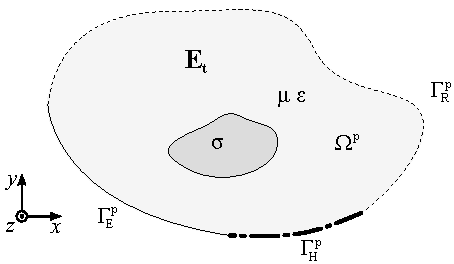
\includegraphics[width=8cm]{FEMproblemEigen} 
\caption{Finite element domain for the waveport eigenvalue problem.}
\label{fig:FEMproblemEigen}
\end{figure}

The electric field distribution $\mathbf{E}$ (at port $p$ on $\Gamma_{WG}$) is computed numerically by solving a \mbox{2-D}\footnote{Similar considerations can be done for $\Omega \equiv \Gamma_{WG}^p \in \mathbb{R}$ to compute excitations in FES-2D.} eigenvalue problem on $\Omega \equiv \Gamma_{WG}^p \in \mathbb{R}^2$ (Fig. \ref{fig:FEMproblemEigen}) using transverse-longitudinal field formulation \cite{zhu2006multigrid}. First, the electric field is expressed as the sum of transverse and longitudinal parts
\begin{equation}
\mathbf{E} = [\mathbf{E}_{t}(x,y) + \hat{\mathbf{z}} \ E_{z}(x,y)] \ \text{e}^{-\gamma z} \quad \text{on } \Omega,
\end{equation}
%
\noindent with $\hat{\mathbf{z}} = -\hat{\mathbf{n}}|_p$ and $\gamma$ is the propagation constant. After the definition of the vector basis functions $\mathbf{v} = \hat{\mathbf{n}}\times\vec{w} \in \mathcal{H}(\mathrm{curl}, \Omega^p, \Gamma_E)$ with $ \mathbf{w} \in \mathcal{W}_{WG} \cap \mathcal{W}_{E}$ such that $\mathbf{E}_{t} = \sum_{j=1}^{N_t} x_{t,j} \mathbf{v}_j$ and the scalar basis functions $\phi \in \mathcal{H}^1(\Omega^p, \Gamma_E)$ such that $E_{z} = \sum_{j=1}^{N_z} x_{z,j} \phi_j$, a Galerkin projection is applied to the eigenvalue problem with isotropic materials governed by
%
\begin{equation}
\nabla \times \frac{1}{\mu_r} \nabla \times \mathbf{E} - {k}_0^2 {\epsilon}_r \mathbf{E} = 0,
\end{equation}
%
\noindent with $\epsilon_r \leftarrow \epsilon_r + {\sigma}/{j\omega_0\epsilon_0}$, leading to the following generalized eigenvalue system of $N_t + N_z$ equations \cite{zhu2006multigrid,jiao2008fast}
\begin{equation}
\label{eq:eigen}
\begin{bmatrix}
{A}_{tt} &0\\
0 &0
\end{bmatrix}
\begin{bmatrix}
\gamma x_{t}\\
x_{z}
\end{bmatrix} = \ \gamma^2
\begin{bmatrix}
{B}_{tt} &{B}_{tz}\\
{B}_{zt} &{B}_{zz}
\end{bmatrix}
\begin{bmatrix}
\gamma x_{t}\\
x_{z}
\end{bmatrix},
\end{equation}
%
\noindent where the matrices entries are given by
\begin{equation*}
\begin{aligned}
A_{tt,ij} &= \int_{\Omega_p} \nabla_t \times \mathbf{v}_i  \cdot \frac{1}{\mu_r} \nabla_t \times \mathbf{v} \ d\Omega \ - \\
 & \qquad k_0^2 \int_{\Omega_p} \mathbf{v}_i  \cdot \epsilon_r \mathbf{v}_j \ d\Omega \ + \\ 
&  \qquad \qquad j k_0 \zeta_0
\int_{\Gamma_R^p} \mathbf{v}_i  \cdot \frac{1}{Z_s} \mathbf{v}_j \ d\Gamma, \\
B_{tt,ij} &= \int_{\Omega_p} \mathbf{v}_i  \cdot  \frac{1}{\mu_r}\mathbf{v}_j \ d\Omega, \\
B_{tz,ij} &= \int_{\Omega_p} \mathbf{v}_i  \cdot  \frac{1}{\mu_r}\nabla_t \phi_j \ d\Omega, \\
B_{zt,ij} &= \int_{\Omega_p} \nabla_t \phi_i  \cdot  \frac{1}{\mu_r}\mathbf{v}_j \ d\Omega, \\
B_{zz,ij} &= \int_{\Omega_p} \nabla_t \phi_i  \cdot  \frac{1}{\mu_r}\nabla_t \phi_j \ d\Omega \ - \\
& \qquad k_0^2 \int_{\Omega_p} \phi_i \epsilon_r \phi_j \ d\Omega \ +\\
& \qquad \qquad j k_0 \zeta_0 \int_{\Gamma_R^p} \phi_i \frac{1}{Z_s} \phi_j \ d\Gamma.
\end{aligned}
\end{equation*}

\noindent $\nabla_t = \hat{\mathbf{x}} \frac{\partial}{\partial x} + \hat{\mathbf{y}} \frac{\partial}{\partial y}$ is the transverse \textit{del} operator.
%

The eigenvalue problem \eqref{eq:eigen}, denoted as $\mat{A}\vect{x} = \lambda \mat{B}\vect{x}$, has $\mat{A}$ and $\mat{B}$ complex symmetric matrices due to the isotropic materials characteristics. The problem can then be solved with a Lanczos-based Krylov subspace solver \cite{farle2004finite} such as the public domain ARPACK solver	\cite{lehoucq1998arpack} in the \textit{shift-invert} mode operation
%
\begin{gather}
\mat{ A-\tau B }^{-1} \mat{B} \vect{x} =  \frac{1}{\lambda-\tau} \vect{x}, \nonumber \\[5pt]
\begin{aligned}
\tau &= k_0^2 \ \epsilon_\text{max} \ \mu_\text{max}, \\
\{\epsilon,\mu\}_\text{max} &= \max\limits_{(x,y)\in\Omega_p} \mathfrak{Re}\left( \{\epsilon,\mu\}(x,y) \right).
\end{aligned} \nonumber
\end{gather}
%
\noindent The shift-invert mode expedites the convergence of the employed iterative process when seeking for largest eigenvalues (lowest cut-off frequencies). Furthermore, spurious modes removal is performed by explicit imposition of $\mat{B}$-orthogonality of the Ritz vectors during the iterative process
%
$$
x_{z}  = - B_{zz}^{-1} B_{zt} \ \gamma x_{t}.
$$
%
Then, the $k^\mathrm{th}$ mode distribution $\mathbf{E}^k$ is normalized such that
%
$$
\int_{\Omega_p}  \mathbf{E}^{k*}  \times  \mathbf{H}^k  \cdot \hat{z} \ d\Omega = 1,
$$
%
\noindent which is achieved upon scaling the unknowns vector such that 
$$ \vect{x} \longleftarrow \frac{\vect{x}}{\sqrt{ \vect{x}^* \mat{B} \vect{x}} }.$$

\subsubsection{Total field scattering}

In this section, the total field scattering formulation is presented in order to treat the electromagnetic scattering from incident waves. We recall the formulation \eqref{eq:FEMform} to incorporate the incident field on the radiation boundary $\Gamma_R$
\begin{multline}
\label{eq:FEMformScatt1}
\int_\Omega \nabla \times \mathbf{w}_i^* \cdot \frac{1}{\mu_r} \nabla \times \mathbf{E} \ d\Omega +
 j k_0 \zeta_0 \int_\Omega \mathbf{w}_i^* \cdot \sigma \mathbf{E} \ d\Omega \ - \\ 
 k_0^2 \int_\Omega \mathbf{w}_i^* \cdot \epsilon_r \mathbf{E} \ d\Omega \ = 
 j k_0 \zeta_0 \int_{\Gamma_{R}} \mathbf{w}_i^* \cdot \hat{\mathbf{n}} \times \mathbf{H} \ d\Gamma, \qquad \forall \mathbf{w}_i \in \mathcal{W}_E.
\end{multline}
%
\noindent The electric and magnetic fields in $\Omega$ can be expressed as the sum of scattered part and an incident part
$$\mathbf{E} = \mathbf{E}^{sc} + \mathbf{E}^{inc}, \qquad \mathbf{H} = \mathbf{H}^{sc} + \mathbf{H}^{inc} $$
\noindent Direct substitution in \eqref{eq:ABC} where the $\mathbf{E} := \mathbf{E}^{sc}$ and $\mathbf{H} := \mathbf{H}^{sc}$ leads to
\begin{eqnarray}
\label{eq:IncBnd}
\hat{\mathbf{n}} \times \mathbf{H} & = & \frac{1}{Z_s} \hat{\mathbf{n}} \times \hat{\mathbf{n}} \times \mathbf{E} + \hat{\mathbf{n}} \times \mathbf{H}^{inc} - \frac{1}{Z_s} \hat{\mathbf{n}} \times \hat{\mathbf{n}} \times \mathbf{E}^{inc}, \qquad \mathrm{on} \ \Gamma_{R}.
\end{eqnarray}
\noindent The first term in right-hand side of \eqref{eq:IncBnd} leads to a radiation boundary integral (canonical first order absorbing boundary condition) while the next two terms will enforce the impinging field values on $\Gamma_R$. As a result
\begin{multline}
\label{eq:FEMformScatt}
\int_\Omega \nabla \times \mathbf{w}_i^* \cdot \frac{1}{\mu_r} \nabla \times \mathbf{E} \ d\Omega + j k_0 \zeta_0 \int_\Omega \mathbf{w}_i^* \cdot \sigma \mathbf{E} \ d\Omega \ + \\
\hspace{-2cm} j k_0 \zeta_0 \int_{\mathrm{\Gamma}_R} \hat{\mathbf{n}} \times \mathbf{w}_i^* \cdot \frac{1}{Z_s} \hat{\mathbf{n}} \times \mathbf{E} \ d\mathrm{\Gamma} \ - 
 k_0^2 \int_\Omega \mathbf{w}_i^* \cdot \epsilon_r \mathbf{E} \ d\Omega \ = \\
 j k_0 \zeta_0 \int_{\Gamma_{R}} \hat{\mathbf{n}} \times \mathbf{w}_i^* \cdot \left( \frac{1}{Z_s} \hat{\mathbf{n}} \times \mathbf{E}^{inc} - \mathbf{H}^{inc} \right) \ d\Gamma, \qquad \forall \mathbf{w}_i \in \mathcal{W}_E.
\end{multline}

\noindent The knowledge of the tangential components of the impinging wave on $\Gamma_R$ is sufficient to compute the total fields in $\Omega$. 
%If we consider a plane wave impinging 


\subsection{Element matrices and system assembly}

Efficient computation \cite{rognes2009efficient} of higher-order finite element matrices can be achieved by quadrature integration, and  mappings of the functions from a reference element to the actual element are used to recover the correct shape functions.

\begin{figure}[h!]
\centering
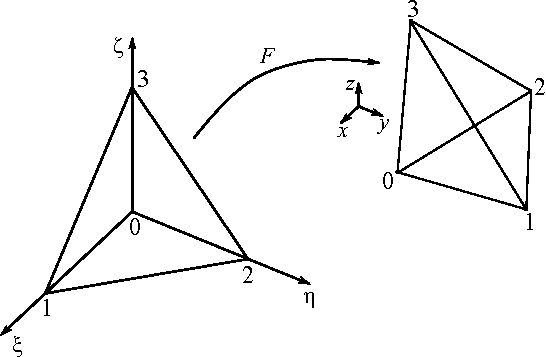
\includegraphics[width=10cm]{MappingTet}
\caption{Linear mapping $F$ of the reference element to the actual element.}
\label{fig:MappingTet}
\end{figure}

Consider the reference and actual elements of Fig. \ref{fig:MappingTet}. There exist a non degenerate affine mapping $F : K_0 \rightarrow K$ from the reference element $K_0$, defined in simplex coordinates $(\xi, \eta, \zeta)$ coordinates, the actual element $K$, defined Cartesian coordinates $(x,y,z)$, defined as
\begin{equation}
\label{eq:mapping}
\begin{bmatrix}
x\\y\\z
\end{bmatrix}
=
\begin{bmatrix}
x_1-x_0 & x_2-x_0 & x_3-x_0\\
y_1-y_0 & y_2-y_0 & y_3-y_0\\
z_1-z_0 & z_2-z_0 & z_3-z_0
\end{bmatrix}
\begin{bmatrix}
\xi \\ \eta \\ \zeta
\end{bmatrix}
+
\begin{bmatrix}
x_0\\
y_0\\
z_0
\end{bmatrix}.
\end{equation}

\noindent The Jacobian matrix $\mat{J}$ of the transformation, defined as
\begin{equation}
\label{eq:jacobian}
\begin{bmatrix}
J
\end{bmatrix}
=
\begin{bmatrix}
\frac{\partial x}{\partial \xi} & \frac{\partial y}{\partial \xi} & \frac{\partial z}{\partial \xi}\\
\frac{\partial x}{\partial \eta} & \frac{\partial y}{\partial \eta} & \frac{\partial z}{\partial \eta}\\
\frac{\partial x}{\partial \zeta} & \frac{\partial y}{\partial \zeta} & \frac{\partial z}{\partial \zeta}
\end{bmatrix},
\end{equation}

\noindent allows for straightforward computation of the partial derivatives of the shape functions: given a scalar function $\phi(\xi, \eta, \zeta)$ on the reference element, its partial derivatives on the actual element can be computed as
\begin{equation}
\label{eq:gradients}
\begin{bmatrix}
\frac{\partial \phi(x, y, z)}{\partial x} \\
\frac{\partial \phi(x, y, z)}{\partial y} \\
\frac{\partial \phi(x, y, z)}{\partial z} 
\end{bmatrix}
=
\begin{bmatrix}
J
\end{bmatrix}^{-1}
\begin{bmatrix}
\frac{\partial \phi(\xi, \eta, \zeta)}{\partial \xi} \\
\frac{\partial \phi(\xi, \eta, \zeta)}{\partial \eta} \\
\frac{\partial \phi(\xi, \eta, \zeta)}{\partial \zeta} 
\end{bmatrix}.
\end{equation}

\noindent Some of the integrals (the $\mathcal{H}(\mathrm{curl},\Omega)$-conforming \textit{stiffness} matrices) we have seen in the previous formulations involve the curls of the shape functions. They can readily be computed upon employing the vector identities $\nabla \times \left( \phi \mathbf{A} \right) = \phi \nabla \times \mathbf{A} + \nabla \phi \times \mathbf{A}$ and $\nabla \times \nabla \phi = 0$ and remembering that the curl operator is linear. The curls of the shape functions of table \ref{tab:Hcurlfunctions} can be recast in functions of the scalar functions and their gradients. Table \ref{tab:curlHcurlfunctions} shows their respective curls.

\begin{sidewaystable}[!]
\begin{center}
\begin{tabular}{|c|c|c|}
\hline 
Rotational basis $\left(\mathcal{H}(\mathrm{curl},\Omega)\right)$ & curl of rotational basis $\left(\mathcal{H}(\mathrm{div},\Omega)\right)$ \\
\hline
\hline 
$\phi_i\nabla\phi_j-\phi_j\nabla\phi_j$  & $2  (\nabla \phi_i \times \nabla \phi_j)$ \\
\hline 
$3\phi_j\phi_k\nabla\phi_i-\nabla(\phi_i\phi_j\phi_k)$ & $3 (\phi_j \nabla \phi_k +  \phi_k \nabla \phi_j ) \times \nabla \phi_i$ \\
$3\phi_k\phi_i\nabla\phi_j-\nabla(\phi_i\phi_j\phi_k)$ & $3 (\phi_k \nabla \phi_i + \phi_i \nabla \phi_k ) \times \nabla \phi_j$ \\
\hline 
$4\phi_j\phi_k(\phi_j - \phi_k)\nabla\phi_i - \nabla\left(\phi_i\phi_j\phi_k(\phi_j-\phi_k)\right)$ & $4\left((\phi_j^2-2\phi_j\phi_k)\nabla\phi_k - (\phi_k^2-2\phi_j\phi_k)\nabla\phi_j \right) \times\nabla\phi_i$ \\
$4\phi_k\phi_i(\phi_k - \phi_i)\nabla\phi_j - \nabla\left(\phi_i\phi_j\phi_k(\phi_k-\phi_i)\right)$ & $4\left( (\phi_k^2-2\phi_k\phi_i)\nabla\phi_i - (\phi_i^2-2\phi_k\phi_i) \nabla\phi_k \right) \times\nabla\phi_j$ \\
$4\phi_i\phi_j(\phi_i - \phi_j)\nabla\phi_k - \nabla\left(\phi_i\phi_j\phi_k(\phi_i-\phi_j)\right)$ & $4\left((\phi_i^2-2\phi_i\phi_j)\nabla\phi_j - (\phi_j^2-2\phi_i\phi_j) \nabla\phi_i\right) \times\nabla\phi_k$ \\
$4\phi_j\phi_k\phi_l\nabla\phi_i - \nabla(\phi_i\phi_j\phi_k\phi_l)$ & $4\left(\phi_k\phi_l\nabla\phi_j + \phi_j\phi_l\nabla\phi_k + \phi_j\phi_k\nabla\phi_l\right)\times\nabla\phi_i$ \\ 
$4\phi_k\phi_l\phi_i\nabla\phi_j - \nabla(\phi_i\phi_j\phi_k\phi_l)$ & $4\left(\phi_l\phi_i\nabla\phi_k + \phi_k\phi_i\nabla\phi_l + \phi_k\phi_l\nabla\phi_i\right)\times\nabla\phi_j$ \\ 
$4\phi_l\phi_i\phi_j\nabla\phi_k - \nabla(\phi_i\phi_j\phi_k\phi_l)$ & $4\left(\phi_i\phi_j\nabla\phi_l+ \phi_l\phi_j\nabla\phi_i + \phi_l\phi_i\nabla\phi_j\right)\times\nabla\phi_k$ \\ 
\hline 
\end{tabular} 
\end{center}
\caption{Curls of $\mathcal{H}(\mathrm{curl},\Omega)$-conforming basis functions up to order $p = 3$.}
\label{tab:curlHcurlfunctions}
\end{sidewaystable}

Finally, the reference element with vertices $N_i, \ i=0,\ldots,3$, in simplex coordinates
\begin{eqnarray*}
N_0 &:= & (0,0,0),\\
N_1 &:= & (1,0,0),\\
N_2 &:= & (0,1,0),\\
N_3 &:= & (0,0,1),
\end{eqnarray*}
\noindent has four scalar (\textit{nodal}) first order shape functions defined as
\begin{eqnarray*}
\phi_0 &= &1 - \xi - \eta -\zeta, \\
\phi_1 &= &\xi, \\
\phi_2 &= &\eta, \\
\phi_3 &= &\zeta.
\end{eqnarray*}
\noindent Considering the linear mapping, the volume integration of a function in $K$ can be transferred to an integration on $K_0$ such that \cite{pelosi2009quick}
%
\begin{equation}
\int_{K} f(x,y,z) \ dx dy dz = \int_{K_0} f(\xi, \eta, \zeta) \ \det\mat{J} \ d\xi d\eta d\zeta,
\end{equation}
%
\noindent where we have made the following transformations
\begin{equation}
\begin{aligned}
\phi(x,y,z) \ & \longrightarrow \ \phi(\xi, \eta, \zeta),\\
\nabla\phi(x,y,z) \ & \longrightarrow \ \mat{J}^{-1} \nabla \phi(\xi, \eta, \zeta).
\end{aligned}
\end{equation}

As stated before, quadrature integration results to be an easy integration method for higher-order shape functions \cite{rachowicz2005hp, zaglmayr2006high}, as a few sampling points of $f(\xi, \eta, \zeta)$ are required to achieve machine precision. %If the order of the function $f(\xi, \eta, \zeta)$ is $2p$, then a Gaussian quadrature requires only $p+1$ points in which the function is evaluated \cite{rachowicz2005hp}. 
As a result,
%
$$\int_{K_0} f(\xi, \eta, \zeta) \ \det\mat{J} \ d\xi d\eta d\zeta \approx \sum_q^{N_q} f(\xi_q, \eta_q, \zeta_q) \ w_q, $$
%
\noindent where $(\xi_q, \eta_q, \zeta_q)$ is the simplex coordinate of the $q^\mathrm{th}$ point in the reference element and $w_q$ the corresponding weight. A set of quadrature rules, which have been implemented in FES-3D, can be found in \cite{keast1986moderate}. These allow to compute all the element matrices of first order with $4$ points, second order with $11$ and third order with $24$ points, resulting in, respectively, $\mathbb{R}^{6\times6}$, $\mathbb{R}^{20\times20}$ and $\mathbb{R}^{45\times45}$ dense matrices. The number of points is actually related to the \textit{mass} matrices, associated to the testing with the non-derived shape functions, which lead to the highest polynomial order for $f(x,y,z)$.

%A numerical approach to construct arbitrary order quadrature rules %can be found in \cite{zhang2009set}. 

Once all the integrals derived from a Galerkin procedure are computed on one element, the coefficients must be added to the global system matrix taking into account, for $\mathcal{H}(\mathrm{curl},K)$ matrices, the direction of the shape function defined on the edges and faces, in order to ensure the effective continuity of tangential components of the field. In fact, adjacent elements may result have opposite vector fields (hence discontinuous) at their interface, due to arbitrary mappings. Local numbering of the elements may be uncorrelated to the global mapping of the mesh.

A simple and elegant manner to enforce continuity is to number the nodes of each element such that the node indices are taken in an increasing way \cite{rognes2009efficient}, for instance
\begin{eqnarray*}
E \lbrace i,j\rbrace & \ \text{with} & \ i < j,\\
F \lbrace i,j,k\rbrace & \ \text{with} & \ i < j < k,\\
T \lbrace i,j,k,l \rbrace & \text{with} & \ i < j < k < l,
\end{eqnarray*}
\noindent where the 2-tuple $E\lbrace i,j\rbrace$ with nodes $i$ and $j$ directed from $i$ to $j$, the 3-tuple $F\lbrace i,j,k\rbrace$ is the face with nodes $i$, $j$ and $k$ and the 4-tuple $T\lbrace i,j,k,l\rbrace$ is the tetrahedron with nodes  $i$, $j$, $k$ and $l$. The face $F\lbrace i,j,k\rbrace$ between two adjacent tetrahedra will have three edges oriented in an unique way on both actual and reference element: $E\lbrace i,j\rbrace $, $E\lbrace i,k\rbrace$ and $E \lbrace j,k\rbrace$. 
\begin{eqnarray*}
E\lbrace i,j\rbrace  & \longrightarrow & E_0\lbrace i_0,j_0\rbrace,\\
E\lbrace i,k\rbrace & \longrightarrow & E_0\lbrace i_0,k_0\rbrace,\\
E \lbrace j,k\rbrace & \longrightarrow & E_0\lbrace j_0,k_0\rbrace,
\end{eqnarray*}
\noindent where $i_0$, $j_0$ and $k_0$ are local indices of the reference element nodes. Same considerations can be made on the faces pertaining to a tetrahedron:
\begin{eqnarray*}
F\lbrace i,j,k\rbrace & \longrightarrow & F_0\lbrace 0,1,2\rbrace,\\
F\lbrace i,j,l\rbrace & \longrightarrow & F_0\lbrace 0,1,3\rbrace,\\
F\lbrace i,k,l\rbrace & \longrightarrow & F_0\lbrace 0,2,3\rbrace,\\
F\lbrace j,k,l\rbrace & \longrightarrow & F_0\lbrace 1,2,3\rbrace,\\[5pt]
T\lbrace i,j,k,l\rbrace & \longrightarrow & T_0\lbrace 0,1,2,3\rbrace.
\end{eqnarray*}

The global numbering of the hierarchical shape functions can be made such that the resulting finite element coefficients are collected by their polynomial order $p$
$$
\begin{bmatrix}
A_{1,1} & A_{1,2} & \ldots & A_{1,p}\\
A_{2,1} & A_{2,2} &  & \vdots\\ 
\vdots & & \ddots & \vdots\\
A_{p,1} & \ldots & \ldots & A_{p,p}
\end{bmatrix}.
$$
\noindent A consequence of this approach is that an efficient $p$-multilevel preconditioner can be built to accelerate iterative solvers on high-order finite element matrices \cite{sun2001construction, ingelstrom2006new}.

The assembly operation, which consists in the summation of finite element coefficients computed from elements that share at least one mesh entity (node, edge or face, depending on the kind of shape functions), is done by mapping a local coefficient to a global mesh entity. In FES, the computation of element matrices and their assembly in global system matrix has been parallelized, on multicore CPU, by the use of the OpenMP \textit{parallel for} directive \cite{chapman2008using}.

\subsection{System solution}

As introduced above, the system matrices are usually large, although they are sparse and symmetric. Therefore, an efficient solution of the finite element
matrix equation is very important, because this aspect typically dominates the overall computer resources requirements. %The important issues are matrix storage schemes, matrix solvers (direct or iterative), and matrix preconditioners (in the iterative case).

The matrices produced by the finite element method are sparse, with only a very small percentage of nonzero elements. By storing only the nonzero entries \cite{shahnaz2005review}, the matrix storage requirement is reduced from $O(N^2)$ to $O(N)$. Popular approaches to sparse matrix storage are those based on either a \textit{compressed row} or a \textit{compressed column} storage format. In these approaches, the nonzero entries of a sparse matrix are stored in a floating-point vector (single or double precision complex entries). In addition, an integer vector is employed to store the row or column indices of the nonzero entries, and another integer vector is introduced to store the location of the first nonzero entry of each row or column in the compressed vector. For a symmetric matrix, only the nonzero entries in the upper or lower triangle (including those on the diagonal) need to be stored. In FES, the use of the template library GMM++ \cite{renard2005gmm++} has allowed for fast and memory efficient global matrix assembly.

The choice of a matrix solver can have a significant impact on the computational efficiency, and it is therefore important to choose a solver that can best exploit the properties of the finite element system matrix. There are two types of matrix solvers:
%
\begin{itemize}
\item the first, known as a \textit{direct solver}, is based on Gaussian elimination, typically after LU or Cholesky decompositions. These solvers are commonly used for full matrices \cite{anderson1995lapack}, although they are also applicable to sparse matrices, namely the \textit{sparse direct solvers}. During the past two decades, remarkable progress has been made on sparse direct solvers. Today, there are many highly robust and efficient direct solvers available that deal with sparse matrices. Among these, Intel's Math Kernel Library (MKL) \cite{intel2013MKL} implements the PARDISO solver \cite{schenk2001pardiso}, a multicore sparse direct solver for both symmetric and unsymmetric matrices. Other, open source solvers, are UMFPACK \cite{davis2004algorithm}, MUMPS \cite{amestoy2001mumps}, and SuperLU \cite{li2011superlu}, which provide a scalable parallel solution on distributed memory computing systems (multiprocessor). FES employs MUMPS, an LU or Cholesky-based (depending on $\mat{A}$ symmetry) sparse direct solver with out-of-core (OOC) capabilities, that is the possibility to store in non-volatile memory the computed factors, while keeping into physical memory only the necessary information for factors being computed. This approach hence allows to solve larger systems than those can fit into physical memory at the expense of reducing the bandwidth to that of the non-volatile support. Recent hardware improvements such as the advent of solid state drives, which have a significantly greater bandwidth than classical (magneto-resistive) hard-drives, may increase the frontiers in direct matrices solution on a simple computer. FES-3D also make use of a multithreaded BLAS, OpenBLAS \cite{OpenBlas}, to enable multicore arithmetic operations for MUMPS. Also, the public package METIS \cite{karypis1995metis} is employed for fill-in reduction (elements entries are reordered to compress them around the diagonal).
%
\item the other, the \textit{iterative solver}, requires significantly less memory than do direct solvers because they are based on calculating successive matrix-vector products according to an iterative algorithm that is designed to converge to the solution \cite{saad2000iterative}. The main drawback of iterative techniques is that they may require a large number of iterations to converge, due primarily to the locations of the eigenvalues of the matrix in the complex plane. However, if the eigenvalues are all clustered around $(1, 0)$, convergence is usually rapid. To improve the convergence of an iterative solver, a preconditioner is typically adopted to move the eigenvalues closer to $(1, 0)$, thereby reducing the iteration count. A preconditioner can be constructed based on physical insight into the problem \cite{greif2007preconditioners} or on the structure of the original matrix \cite{kechroud2004preconditioning}. For iterative solvers, SPARSKIT \cite{saad1994sparsekit} provide a variety of Krylov subspace algorithms, such as those based on the stabilized \textit{biconjugate gradient squared} (BiCGStab) and \textit{generalized minimal residual} (GMRES) methods, and a variety of preconditioners, such as the \textit{incomplete LU} (ILU) and its threshold dropping version ILUT \cite{saad1994ilut}, and \textit{successive over relaxation} (SSOR) preconditioners, to speed up the iterative convergence. Note that MKL also contains sparse iterative solvers. FES-3D implements the \textit{restarded}-GMRES solver \cite{barrett1994templates} mainly employed with the domain decomposition preconditioner as it will be shown in \ref{chap:DD}. The advantage of this Krylov subspace solver is that the number of vectors spanning the solution can be restricted to a \quotes{restarting} number $r$, and the Krylov spanning vectors of the successive GMRES cycle (as convergence may not be achieved within $r$ iterations) are computed at from a starting vector which is the solution achieved at the previous GMRES cycle. This approach does not mathematically guarantee the convergence of the solver (due to restarting), however it has been found to be effective in all the analyses performed with FES-3D, at the expense of increasing the number of iterations.
\end{itemize}


\subsection{Post processing}

In the section of the finite element formulation, one of the relevant parameters in the analysis of electromagnetic structures with waveguide excitations have been introduced: the scattering parameters or \textit{$S$-parameters}. Once the finite element matrix has been solved, these can be be obtained after further testings of the field with the mode distributions on $\Gamma_{WG}$. The transfinite element method is such that these testings are incorporated in the system matrix, and hence the $S$-parameters are retrieved during the system solution. A noticeable advantage of the finite element method is that all the ports of an electromagnetic device or antenna array are coupled by means of the finite element interactions, allowing thus for a rigorous analysis of multiple antennas interactions or the accurate response of a microwave device.

When analyzing antennas, several parameters are of a paramount importance in order to define their performances. Some of these are the antenna \textit{directivity} or the \textit{gain}, which are related to the capability of the antenna to radiate fields in a given direction $\hat{\mathbf{r}}$ far away ($kr\gg\lambda$) from the antenna. One can think of an antenna as the medium of transition of an impinging field in the excited port to the free space. Hence, one has to compute the field radiated far away from the antenna in direction $\hat{\mathbf{r}}$. But with the finite element method, we have restricted the domain of analysis to the surrounding of the antenna. However, we can use the Huygens' principle, which states that fields computed on a bounded surface or an advancing front of a propagating wave can be used to compute the next wave-front and so on. Also, it can be proved that tangential fields on any regular bounding surface are sufficient to compute the radiated fields \cite{rothwell2009electromagnetics}. Hence, the tangential components of the fields $\mathbf{E}\times\hat{\mathbf{n}}$ and $\hat{\mathbf{n}}\times\mathbf{H}$ must be known only on $\Gamma_R$. In fact, there might be power flowing through Robin boundaries, which enforce the continuity of waves, whereas Dirichlet or Neumann boundaries are such all the power is reflected on them.

By Sommerfeld's radiation condition states that far-zone fields in the direction $\hat{\mathbf{r}}$, assuming free-space propagation, behave as
$$(\nabla \times \mathbf{E}(\hat{\mathbf{r}})) \times \hat{\mathbf{r}} + j k_0 \mathbf{E}(\hat{\mathbf{r}}) \stackrel{ r \rightarrow \infty}{\approx} 0,$$
\noindent and hence the following relation between the fields can be obtained
$$ \mathbf{E}(\hat{\mathbf{r}}) = \zeta_0 \mathbf{H}(\hat{\mathbf{r}}) \times  \hat{\mathbf{r}}.$$
\noindent This means the fields behave locally as plane wave, that is the electric and magnetic field are orthogonal and they are both orthogonal to the propagating direction $\hat{\mathbf{r}}$. The corresponding Poynting vector,
$$ \mathbf{S}(\hat{\mathbf{r}}) = \frac{1}{2} \mathbf{E}^*(\hat{\mathbf{r}}) \times \mathbf{H}(\hat{\mathbf{r}}) \stackrel{ r \rightarrow \infty}{=} \frac{|\mathbf{E}(\hat{\mathbf{r}})|^2}{2 \zeta_0}\hat{\mathbf{r}}, \qquad \left[\frac{\mathrm{W}}{\mathrm{m}^2}\right],$$
\noindent provides the electromagnetic power density flowing in that direction. To compute the Poynting vector, only the knowledge of the far-zone electric field is required, and it can be computed through Stratton-Chu relations \cite{orfanidis2002electromagnetic} written in Kottler's form in order to remove the gradients of the free-space Green's function. The resulting integral must be computed in
\begin{eqnarray}
\label{eq:Efar}
{\mathbf{E}}(\hat{\mathbf{r}}) &=  &j\zeta_0k_0 \frac{\mathrm{e}^{-jkr}}{4\pi r} \int_{\Gamma_R}  \mathrm{e}^{jk \hat{\mathbf{r}} \cdot \mathbf{r}'} \left [ \left ( \hat{\mathbf{n}}\times\mathbf{H}(\mathbf{r}') \cdot \hat{\mathbf{r}} \right ) \hat{\mathbf{r}} - \hat{\mathbf{n}}\times\mathbf{H}(\mathbf{r}') \right ] \ d\Gamma \ - \nonumber \\ 
& & \qquad jk_0 \frac{\mathrm{e}^{-jkr}}{4\pi r} \int_{\Gamma_R} \mathrm{e}^{jk \hat{\mathbf{r}} \cdot \mathbf{r}'} \ \mathbf{E}(\mathbf{r}')\times\hat{\mathbf{n}}  \times \hat{\mathbf{r}}  \ d\Gamma,
\end{eqnarray}
\noindent where $\mathbf{r}'$ is a vector pointing to the surface $\Gamma_R$. The integral relation \eqref{eq:Efar} can be computed with quadrature rules over the triangles that constitutes the boundary $\Gamma_R$, as the solution of the finite element system provides the electric and magnetic (through \eqref{eq:waveeqErecH}) fields in $\Omega$.
%
\noindent Finally, directivity $D(\hat{\mathbf{r}})$ and gain $G(\hat{\mathbf{r}})$ are computed by
%
\begin{eqnarray}
\label{eq:Dir}
D(\hat{\mathbf{r}}) &= & \lim_{r\to\infty} 4 \pi r^2 \frac{\mathbf{S}(\hat{\mathbf{r}})\cdot \hat{\mathbf{r}}}{P_\mathrm{rad}} = \lim_{r\to\infty} 2 \pi r^2 \frac{|\mathbf{E}(\hat{\mathbf{r}})|^2}{\zeta_0 P_\mathrm{rad}},\\
\label{eq:Gain}
G(\hat{\mathbf{r}}) &= & \lim_{r\to\infty} 4 \pi r^2 \frac{\mathbf{S}(\hat{\mathbf{r}})\cdot \hat{\mathbf{r}}}{P_\mathrm{in}} = \lim_{r\to\infty} 2 \pi r^2 \frac{|\mathbf{E}(\hat{\mathbf{r}})|^2}{\zeta_0 P_\mathrm{in}}, 
\end{eqnarray}
%
\noindent where $P_\mathrm{rad}$ is the power flowing through $\Gamma_R$ computed as
$$P_\mathrm{rad} = \int_{\Gamma_R} \mathbf{E}^*\times\mathbf{H} \cdot \hat{\mathbf{n}} \ d\Gamma,$$
\noindent and $P_\mathrm{in}$ is the total power entering in $\Omega$ through $\Gamma_{WG}$
$$P_\mathrm{in} = - \int_{\Gamma_{WG}} \mathbf{E}^*\times\mathbf{H} \cdot \hat{\mathbf{n}} \ d\Gamma.$$
\noindent Once the $S$-parameters are known, $P_\mathrm{in}$ can be retrieved upon computing
$$P_\mathrm{in} = \sum_{k=1}^{N_{M}^\mathrm{feed}} 1-|S_{kk}|^2,$$
\noindent where $N_{M}^\mathrm{feed}$ is the actual number of modes feeding the electromagnetic structure through $\Gamma_{WG}$. Note that the limit ${r\to\infty}$ in \eqref{eq:Dir} and \eqref{eq:Gain} can be removed upon neglecting the term $\nicefrac{\mathrm{e}^{-jkr}}{r}$ in \eqref{eq:Efar}.

In electromagnetic wave scattering problems, the \textit{(bistatic) radar cross section} $RCS$ provides information on how an object (or electromagnetic structure in $\Omega$) scatters the electromagnetic field coming from an impinging plane wave, and is defined as
\begin{equation}
\label{eq:RCS}
RCS (\hat{\mathbf{r}}) = \lim_{r\to\infty} 4 \pi r^2 \frac{|\mathbf{E}(\hat{\mathbf{r}})|^2}{|\mathbf{E}^{inc}|^2}.
\end{equation}

At last but not least, one might be interested in recovering the field values in each point $\mathbf{r} \in \Omega$. This can be done upon retrieving the element of the mesh that contains $\mathbf{r}$ (with efficient algorithms such as octrees \cite{szeliski1993rapid}) and remembering that
$$\mathbf{E}_E(\mathbf{r}) := \sum_{j=1}^{N} x_j \mathbf{w}_j(\mathbf{r}),$$
\noindent and 
$$\mathbf{H}_E(\mathbf{r}) := \sum_{j=1}^{N} x_j \frac{\nabla \times \mathbf{w}_j(\mathbf{r})}{-j k_0\zeta_0\mu_r(\mathbf{r})}.$$
%
\noindent The local support of $\mathbf{w}_j(\mathbf{r})$ is such that 
\begin{equation}
\mathbf{w}_j(\mathbf{r}) = \left\lbrace
\begin{array}{cc}
\mathbf{w}_j(\mathbf{r}), & \mathbf{r} \in K,\\
0, & \mathbf{r} \not\in K,\\
\end{array}
\right.
\end{equation}
\noindent where $K$ is any element of the mesh.
Notice that for $\mathbf{r}$ located on the face shared by two elements, the tangential components are continuous, hence equal, but normal components may not. We may approximate the normal component as the average of the normal components computed in both elements. In FES-3D, the evaluation of \eqref{eq:Efar} has been parallelized with OpenMP for the look angles $\hat{\mathbf{r}}$. 

Visualization of electromagnetic quantities in higher-order finite elements, is a computationally demanding step. In fact, most of the rendering environments (DirectX, OpenGL,...) which directly communicate with the GPU interpolate linearly quantities to display. Hence one must increase the number of sampling points of the fields in order to accurately visualize them. 

FES, at this stage, samples the fields at the nodes of the mesh and generates a \textit{Visualization ToolKit} (VTK) file \cite{VTK4}, an open format for scientific visualization. In particular, packages (ParaView, MayaVi) that adopt this format allow for visualization of scalars and vectors on structured or unstructured 2D or 3D meshes. Also, operations such as cutting planes, contours plotting, arithmetics might be available. For orders $p=2$ and $3$, the mesh is refined (Fig. \ref{fig:Refinement}) before evaluation of the fields, generating much more sampling nodes. An efficient procedure might be based on oversampling only where the fields vary rapidly, based on error estimation \cite{remacle2007efficient}. 

\begin{figure}[ht!]
\centering
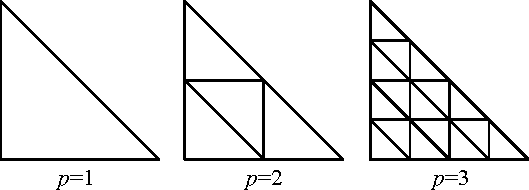
\includegraphics[width=8cm]{Refinement}
\caption{Homogeneous refinement for higher-order finite elements solution visualization.}
\label{fig:Refinement}
\end{figure}

\section{Numerical tests}

This section presents the analysis of four different 3D microwave problems analyzed by FES-3D with the respective comparisons with HFSS (version 10) models:
\begin{itemize}
\item a millimeter-wave E-plane bandpass filter \cite{bui1984broad},
\item a Ka-band corrugated circular horn tailored for radio-astronomy \cite{lucci2005corrugated}, 
%\item a 2.4 GHz, single feed circular polarization patch antenna \cite{maddio2011new},
\item a simple perfect electric scattering sphere.
\end{itemize}

The purpose these tests is to validate the capabilities of the formulations implemented and show some of the features of FES. The core of FES will be extended in the next chapters, where a domain decomposition methods and harmonic balance for nonlinear analyzes of microwave devices will be presented. Current computations are made on AMD Phenom II X4 965 processor with 16 GB of available DDR3 physical memory.

\subsection{Millimeter-wave E-plane bandpass filter analysis}

\begin{figure}[ht!]
\centering
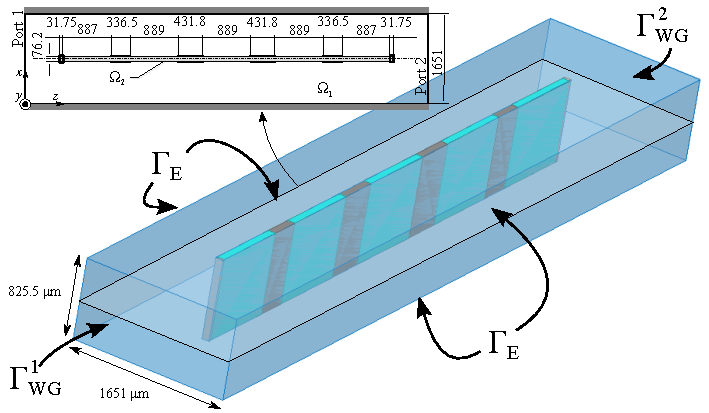
\includegraphics[width=13.4cm]{Bui1984}
\caption{Sketch for the millimeter-wave waveguide filter analyzed and its cross section (H-plane). Measures are given in $\mu m$. }
\label{fig:Bui1984}
\end{figure}

The passband filter designed and presented in \cite{bui1984broad} is realized
by placing on the E-plane a dielectric slab ($\epsilon_r = 2.1$ in $\Omega_2$) partially metalized on both sides in a WR6 rectangular waveguide (Fig. \ref{fig:Bui1984}). All metallic parts will be considered in the FE model as perfect electric conductor. The remaining of the device is devoid of air.

The mesh is composed of 9,686 tetrahedra (not visible here) for a total of 2,074 conjunction nodes. The mesh assembly, with second order basis functions, required about 1.3~s for each frequency of analysis. The boundary conditions where then imposed on the waveports considering both the formulations presented in the previous section. Each 2D eigenmode problem, with second order basis functions, could be solved in approximately 0.4~s. The ARPACK solver, using MUMPS for matrices inversion in the $\mat{B}$-orthogonalization, converged in only 19 iterations (to $10^{-12}$). The dominant mode formulation lead to 57,524 unknowns for a full second order assembly while the transfinite element required less, 56,490 unknowns, as the unknowns on the waveports where removed from the system matrix. 
The overall assembly and solve times where, with the single precision solver, about 5.5~s (2.3~s + 3.2~s) and requiring 132~MB of memory. The double precision solver required approximately the same times, while about twice the memory (255~MB) was needed. Notice that HFSS required only 2~s and about 130~MB of memory for this problem. This could be imparted mainly to the fact it employs a mixed precision solver \cite{sun2008high} for real matrices (in fact they are as no material losses or absorbing boundary conditions are introduced). This kind of solvers iteratively refines the solution provided by a single precision solver $\vect{x}_\mathrm{s}^i =\mat{A}_\mathrm{s}^{-1}\vect{b}_\mathrm{s} \rightarrow \vect{x}_\mathrm{d}^i$ , upon computing a double precision residual vector $\vect{r}_\mathrm{d} = \vect{b}_\mathrm{d} - \mat{A}_\mathrm{d}\vect{x}_\mathrm{d}^i$. Then, the problem on the residual ($\vect{r}_\mathrm{d} \rightarrow \vect{r}_\mathrm{s}$) is solved and added to the double precision solver: $\vect{x}_\mathrm{d}^{i+1} \leftarrow \vect{x}_\mathrm{d}^i + \mat{A}_\mathrm{s}^{-1}\vect{r}_\mathrm{s}$. $s$ and $d$ subscripts correspond, respectively, to single and double precision versions of the matrices or vectors. Furthermore, the use of real matrices noticeably reduce the computational requirements. However, as the purpose of the implemented package is to introduce new computational methodologies, for instance domain decomposition and nonlinear analyzes, the use of real solvers (available with MUMPS) has not been implemented yet.

\begin{figure}[ht!]
\centering
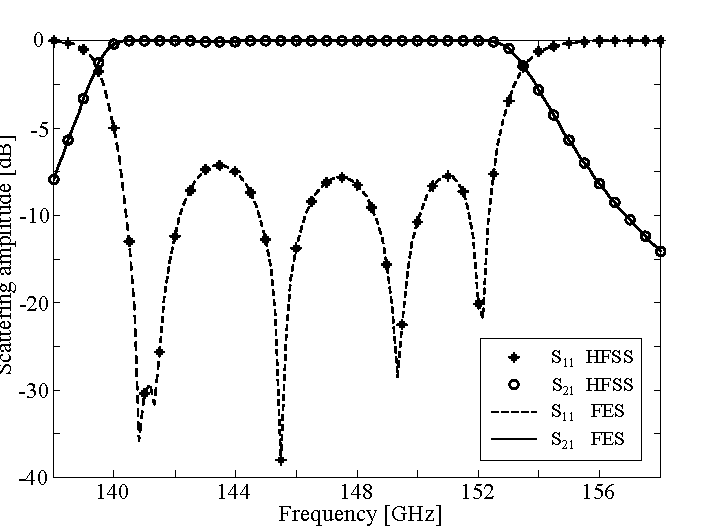
\includegraphics[width=10cm]{Bilat3Dresponse}
\caption{Frequency response of the dominant $\mathrm{TE}_{10}$ mode in the filter, computed with single precision MUMPS solver and dominant mode waveports boundary condition.}
\label{fig:Bilat3Dresponse}
\end{figure}

The frequency (linear) response of the filter, computed with the single precision solver with dominant mode boundary condition on ports, visibly results to be in good agreement with HFSS. In fact, as single precision solver has a numerical error floor of $\approx 10^{-6}$, the dynamic response of the device ($\approx -40~\mathrm{dB} ~\mathrm{to}~0~\mathrm{dB}$) could fit in the dynamic range of numerical precision.

\begin{table}[h!]
\begin{center}
\begin{tabular}{|c|c|c|c|}
\hline 
Dominant (s) & Dominant (d) & Transfinite (s) & Transfinite (d) \\ 
\hline
\hline
$   1.5351 \ 10^{-6}$ & $1.3643 \ 10^{-6}$ & $5.6383 \ 10^{-7}$ & $1.6853 \ 10^{-12}$ \\ 
\hline 
\end{tabular}
\end{center}
\caption{Comparison between the average Euclidean errors for both waveport continuity formulations (only dominant $\mathrm{TE}_{10}$ mode retained), varying the solver precision (s=single, d=double).}
\label{tab:Bilatprecision}
\end{table}

Table \ref{tab:Bilatprecision} shows the relative error $\mathcal{L}^2\left(\mat{S(f)}, \ f\in [138,158]~\mathrm{GHz}\right)$ between the four combinations of waveports formulations and solvers precisions and the solution provided by the mixed precision (real) solver of HFSS in discrete sweep mode. The error is averaged on the 41 equally spaced selected frequency points within the range specified. As we can see, the lower accuracy of the dominant mode formulation is such that a double precision solver does not improve computations. Nevertheless, there no practically appreciable differences between the responses (Fig. \ref{fig:Bilat3Dresponse}). The transfinite element formulation, being more robust, is such that equivalence in results is achieved within numerical precision.


\begin{figure}[h!]
\centering
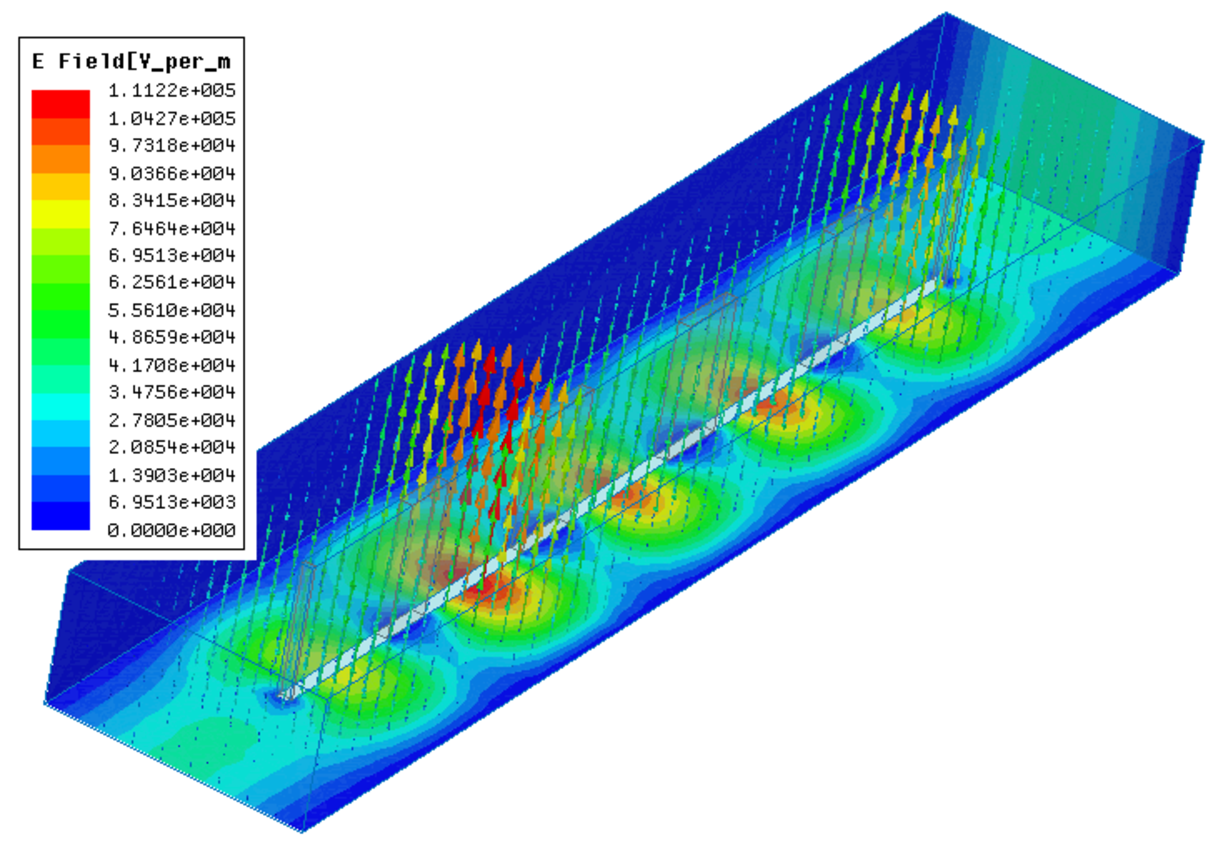
\includegraphics[width=13.4cm]{Bilat3DHFSS}
\caption{Electric field at 150 GHz computed by means of HFSS.}
\label{fig:Bilat3DHFSS}
\end{figure}

\begin{figure}[h!]
\centering
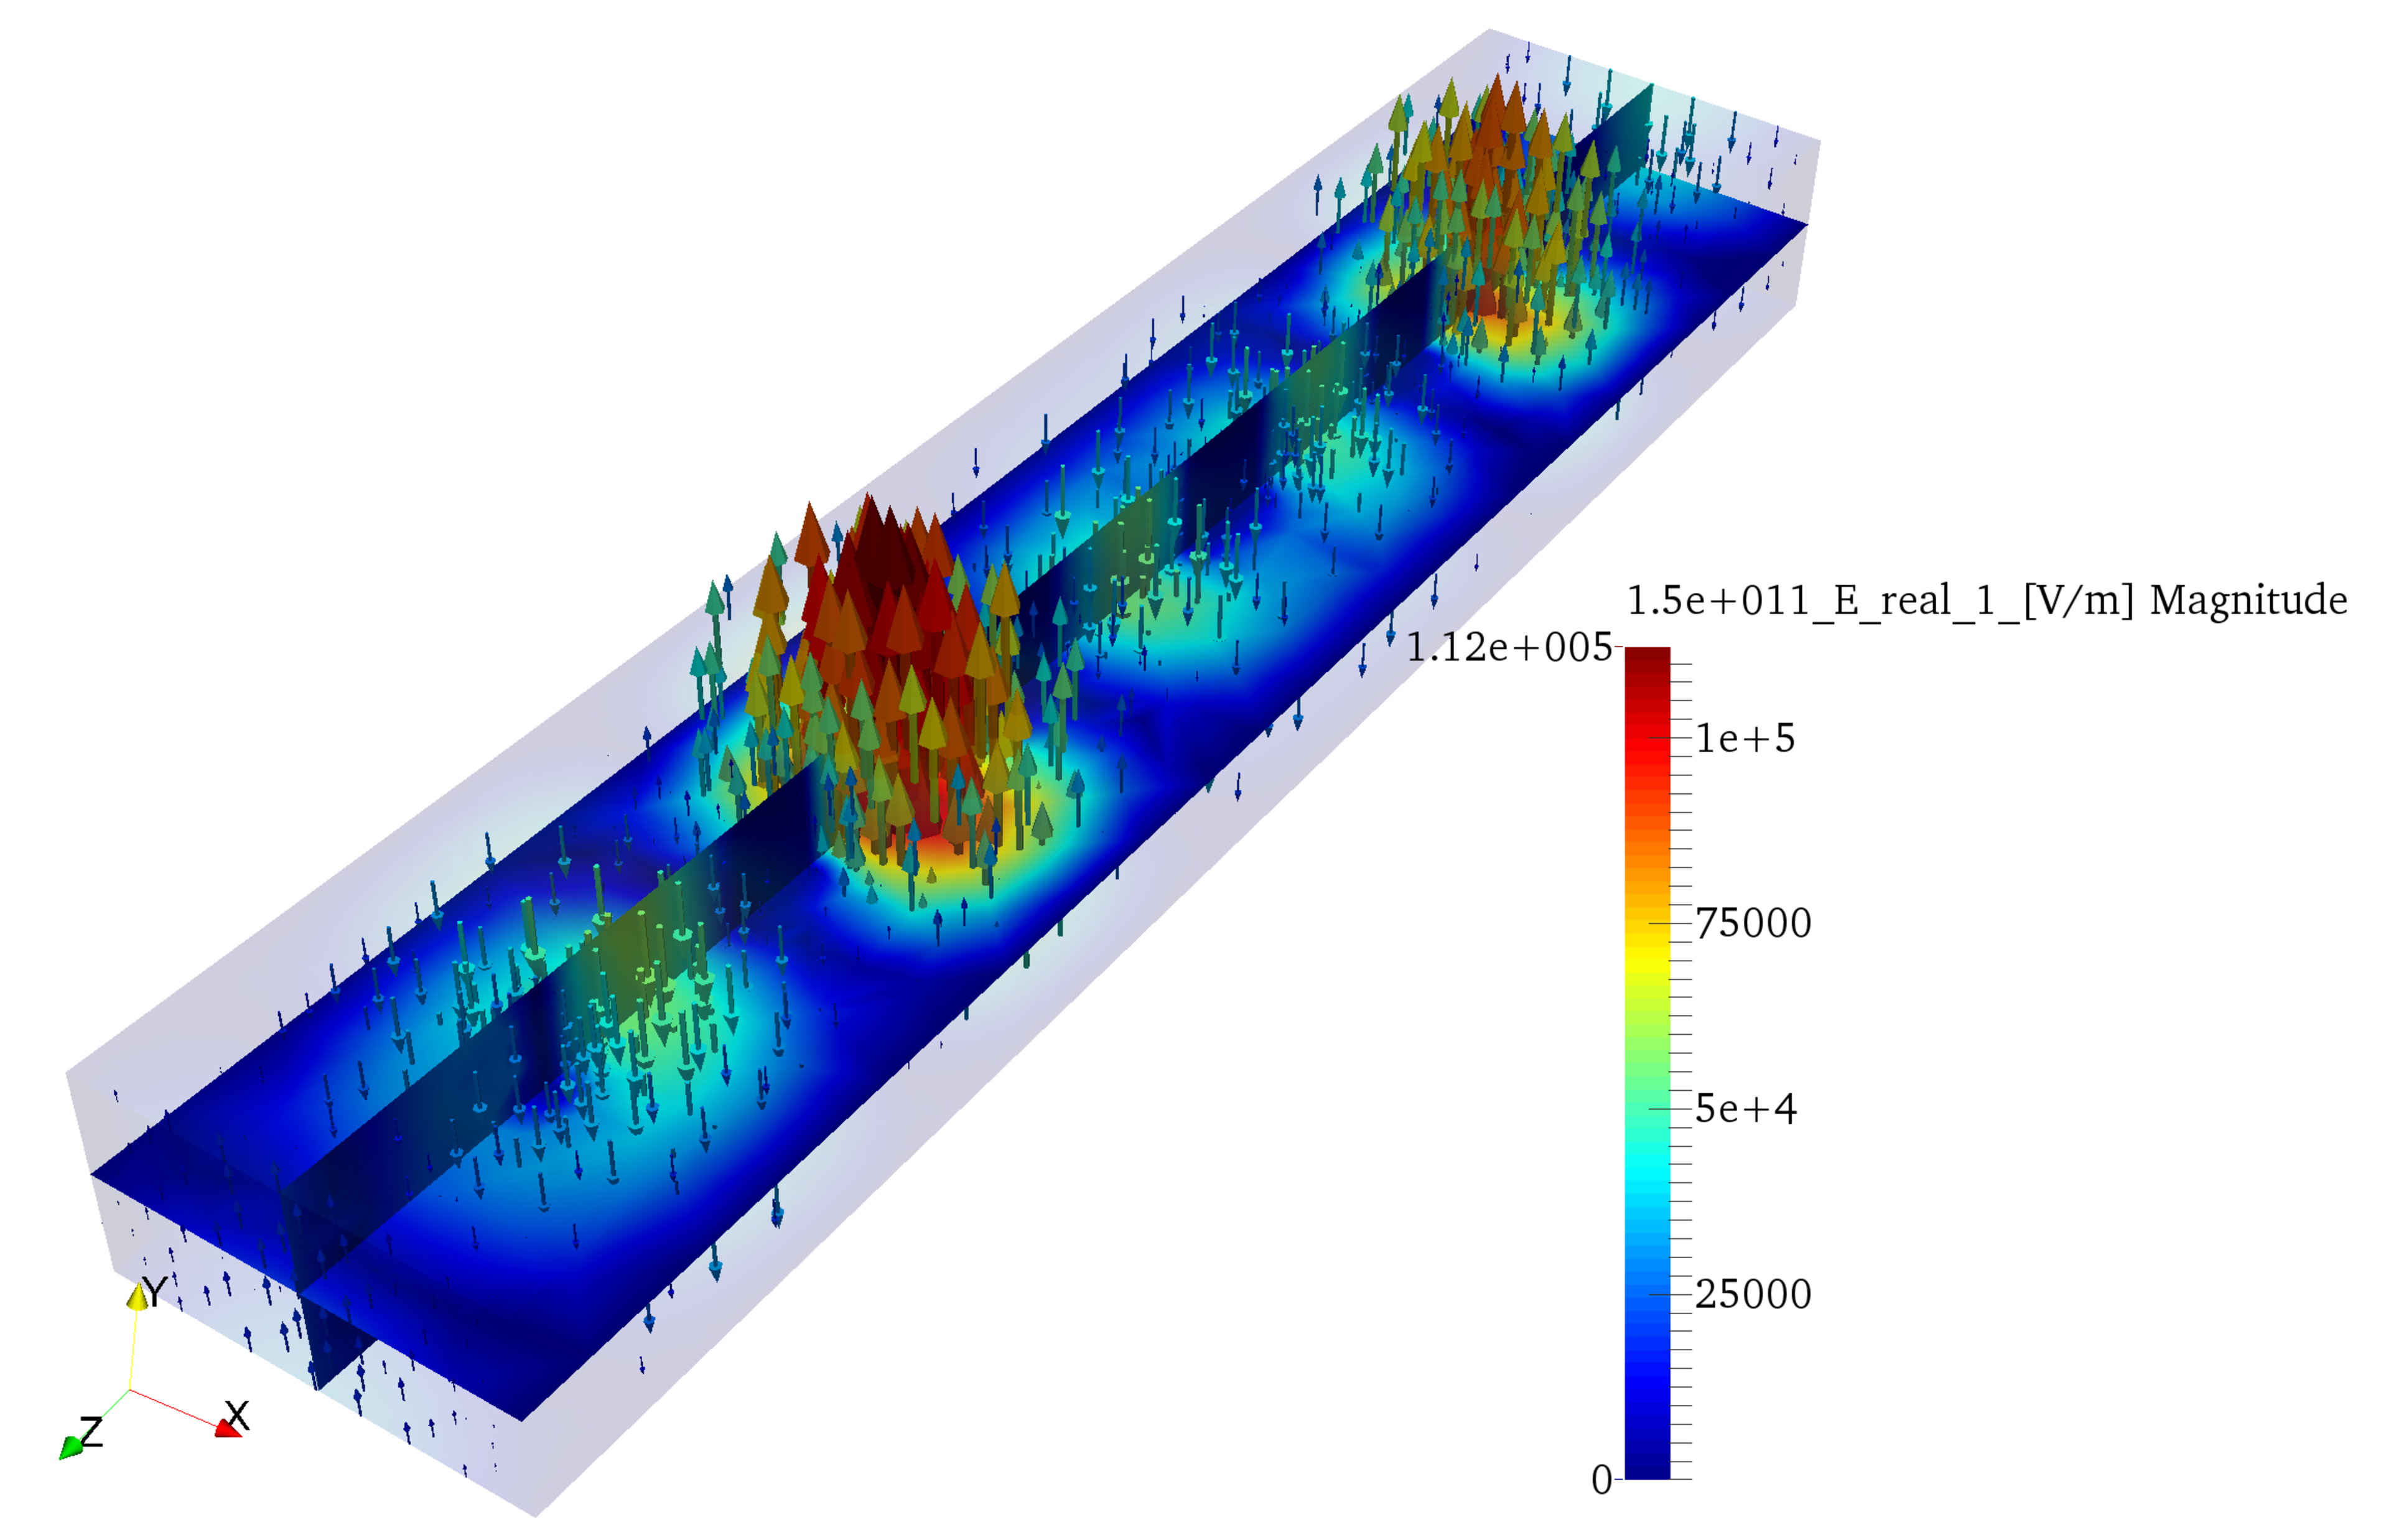
\includegraphics[width=13.4cm]{Bilat3D}
\caption{Electric field at 150 GHz computed by means of FES and visualized in Paraview.}
\label{fig:Bilat3D}
\end{figure}

After the computation of scattering parameters, one might be interested in visualizing the fields at a given frequency. Figs. \ref{fig:Bilat3DHFSS} and \ref{fig:Bilat3D} show the electric fields (real parts) computed at 150~GHz. The electric and magnetic fields, in FES, are computed upon interpolating the respective shape functions at the nodes of the mesh (refined in this case as $p=2$). There is a good agreement between the two electromagnetic solvers and maximum amplitude of the electric field of $\approx 112~\frac{\mathrm{kV}}{\mathrm{m}}$ is attained within the device. Vertical and horizontal cut-planes can be easily obtained in Paraview upon selecting the \quotes{slicing} function. 

\subsection{Corrugated circular horn analysis} \label{sec:Horn}

\begin{figure}[ht!]
\centering
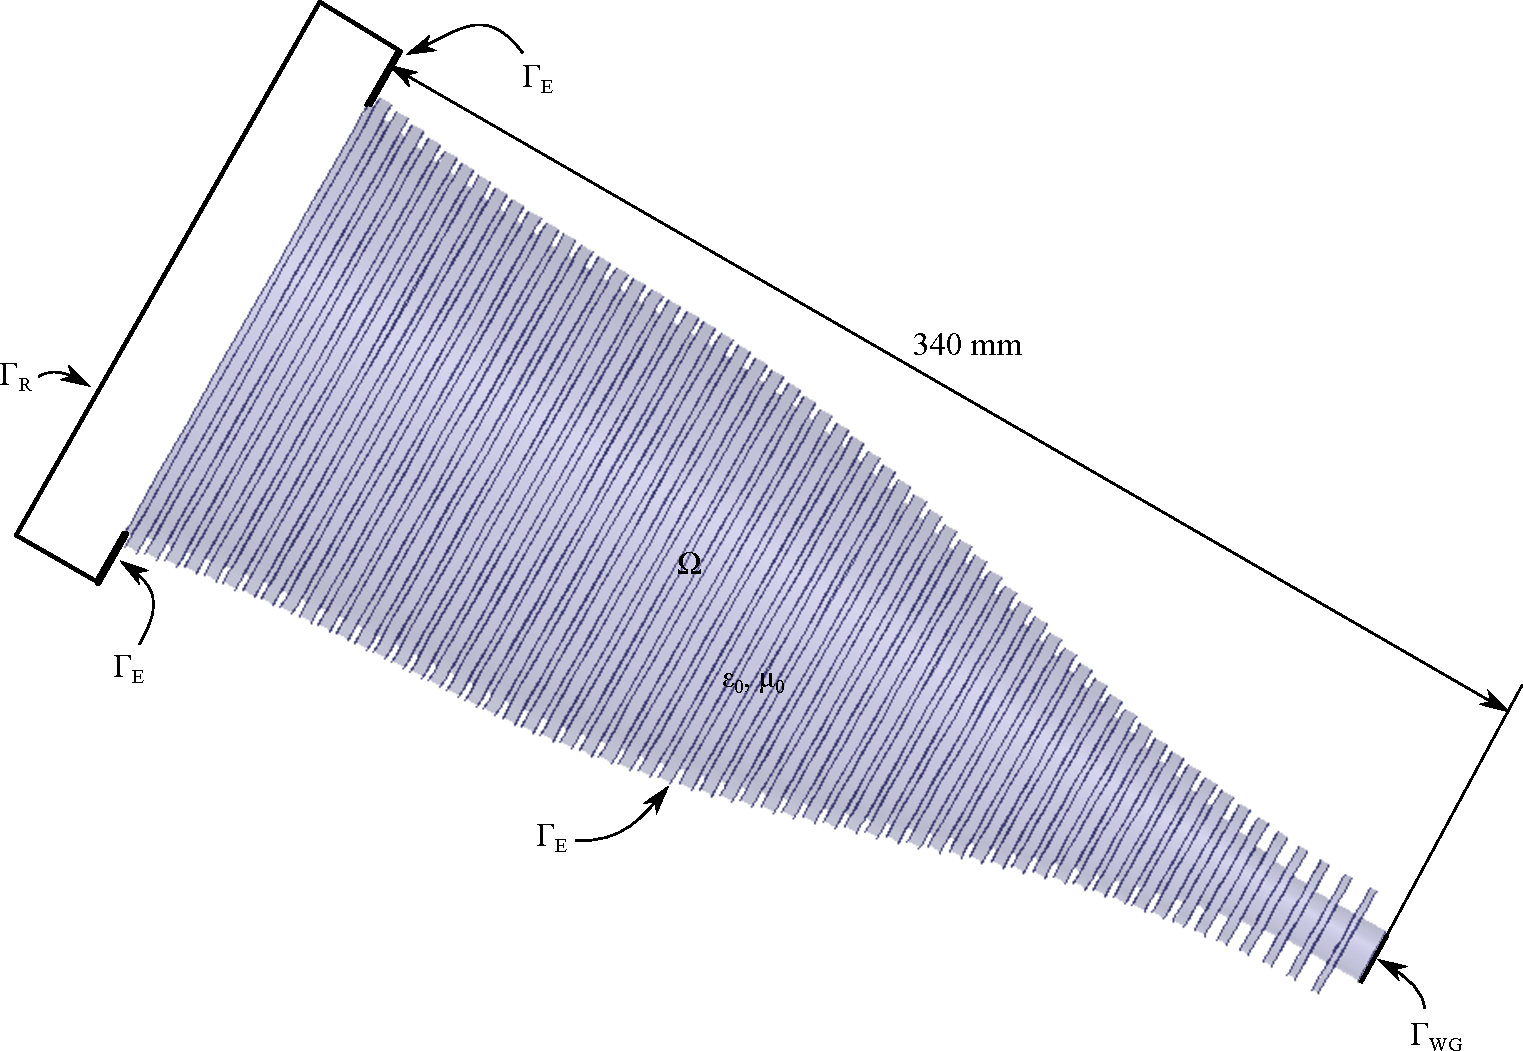
\includegraphics[width=13.4cm]{CircHornSketch}
\caption{Sketch of the 22 GHz corrugated circular horn antenna.}
\label{fig:CircHornSketch}
\end{figure}

In the work \cite{lucci2005corrugated}, there were shown a 22~GHz corrugated circular horn antenna built at the \quotes{Osservatorio Astrofisico di Arcetri}, an institute for radio-astronomical studies of the (Italian) National Research Council. That horn,  whose model is depicted in Fig. \ref{fig:CircHornSketch}, is made of 60 corrugations in order to smooth gradually the transition between guided waves to radiated waves and achieve a pure linear polarization. This procedure results in a better tapering of the radiation pattern, significantly lowering the side lobes. In its designed working conditions, the horn is fed with two degenerate $\mathrm{TE}_{11}$ circular waveguide modes in quadrature: they are both physically oriented perpendicularly and with 90\textdegree~of phase shift.

Here, we have tested the capabilities of FES to analyze multimode problems, with the transfinite element method, and it is a first attempt to evaluate radiation boundary conditions. Notice that antenna is about 25 wavelengths long and the corrugations dramatically increase tetrahedra's number of the mesh, for conformity constraints to the geometry.  The antenna is terminated at its narrower end by a circular waveport boundary and at the mouth or aperture of the horn, by a parallelepiped box on which radiation conditions are imposed. Of course, both horn and box are merged in order to have a unique enclosed medium devoid of air. Simulations are performed with cubic order shape functions.

\begin{figure}[ht!]
\centering
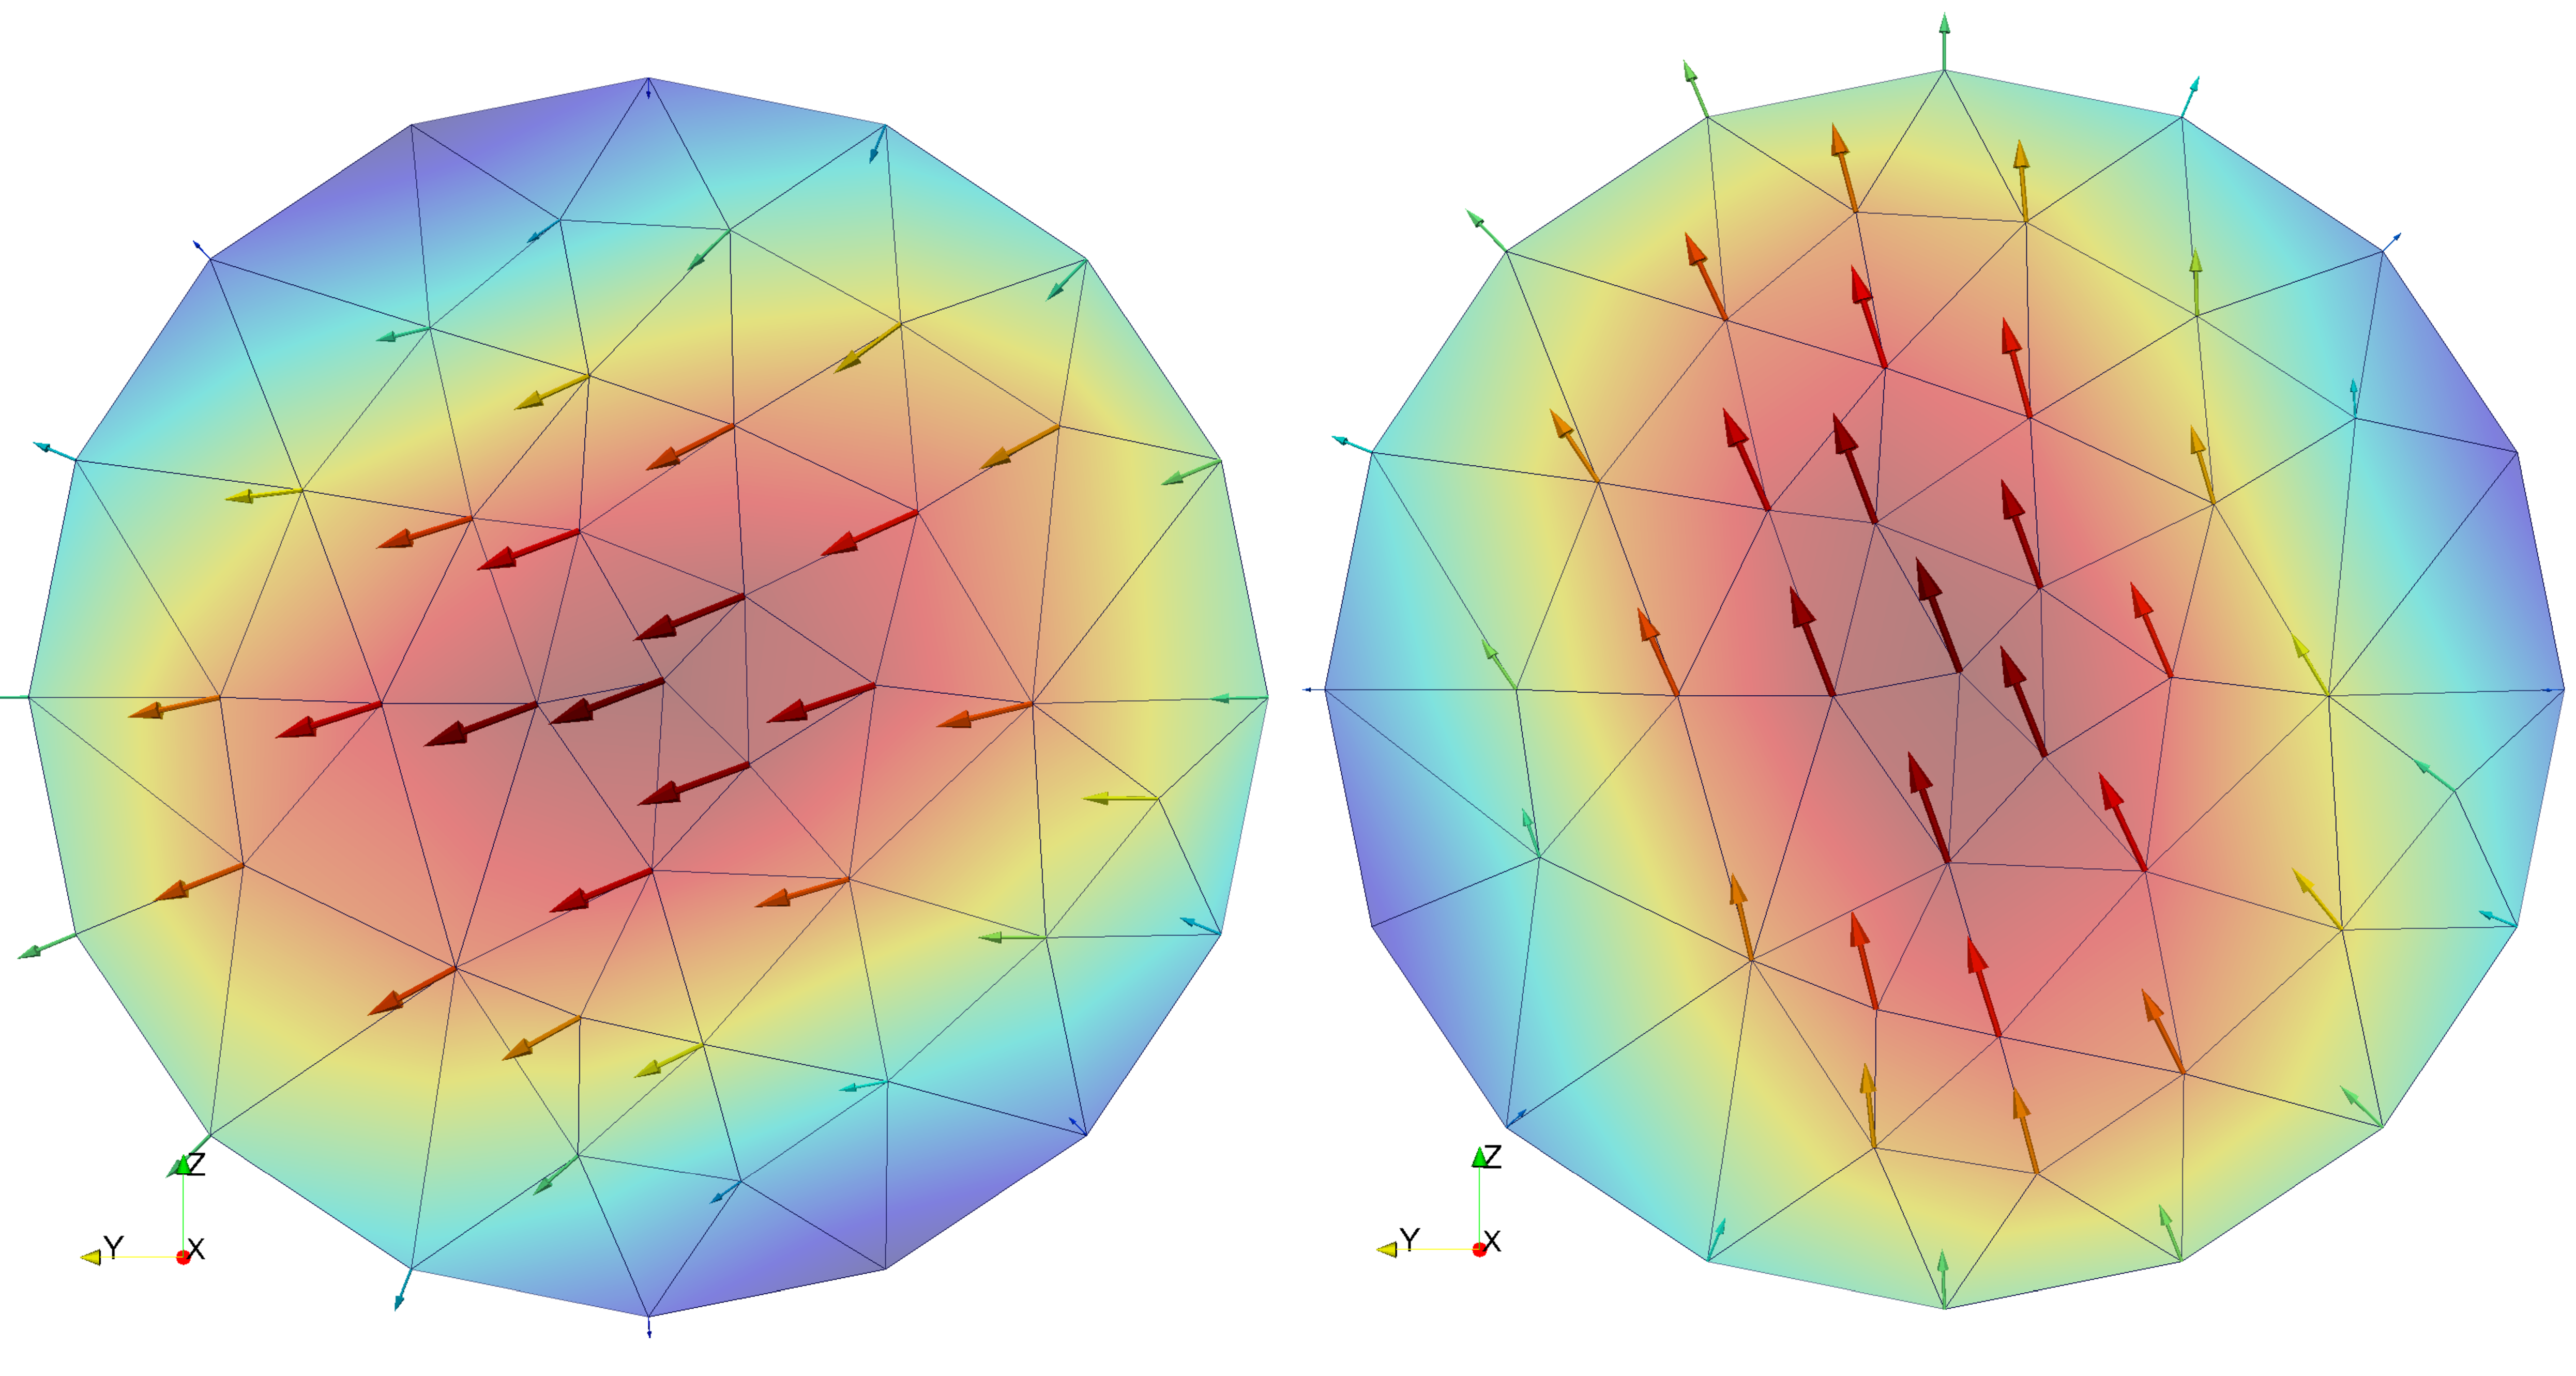
\includegraphics[width=8cm]{Modes}
\caption{Degenerate $\mathrm{TE}_{11}$ modes feeding the antenna (in quadrature).}
\label{fig:Modes}
\end{figure}


The first five modes were computed with ARPACK, and 36 iterations where needed to converge in about 2~s. The excitation modes are shown Fig. \ref{fig:Modes}. Then the assembly and solve on 602,594 unknowns (36,331 tetrahedra) required for the single precision solver about 123~s while the double precision 170~s. In fact, as both the matrices are assembled in the double precision, the single precision solver required 47~s less than its double precision counterpart. Also, memory requirements where different: 3,158~MB for the single precision and 6,159~MB for the double. Notice that HFSS required 146~s and 3.7~GB of memory to solve the problem with its mixed precision complex solver, which is in good agreement with what was stated before.

\begin{eqnarray*}
|\mat{S}|_\mathrm{dB}^\mathrm{HFSS} & = &
\begin{bmatrix}
  -49.7001 & -60.5669 & -55.9466 & -82.8433 & -79.8956 \\
  -60.5669 & -49.9378 & -46.5148 & -87.5034 & -81.1233 \\
  -55.9460 & -46.5148 &  -3.4413 & -80.8478 & -86.5927 \\
  -82.8433 & -87.5033 & -80.8478 & -48.4840 & -88.2707 \\
  -79.8958 & -81.1234 & -86.5927 & -88.2707 & -48.3815
\end{bmatrix},\\
|\mat{S}|_\mathrm{dB}^\mathrm{TFE,single} & = &
\begin{bmatrix}
  -49.0035 & -63.4025 & -64.6486 & -80.1454 & -80.7432 \\
  -63.2030 & -49.6485 & -46.1201 & -91.9744 & -82.0608 \\
  -64.4864 & -46.1409 &  -3.4416 & -81.8164 & -84.3125 \\
  -80.1613 & -91.9789 & -81.8047 & -48.5274 & -91.8034 \\
  -80.7334 & -82.0586 & -84.3199 & -91.8016 & -48.3397
\end{bmatrix},\\
|\mat{S}|_\mathrm{dB}^\mathrm{TFE,double} & = & 
\begin{bmatrix}
  -49.1332 & -63.1736 & -64.5808 & -80.1579 & -80.7213 \\
  -63.1736 & -49.9021 & -46.1233 & -92.0040 & -82.1035 \\
  -64.5808 & -46.1233 &  -3.4414 & -81.8144 & -84.1136 \\
  -80.1579 & -92.0040 & -81.8144 & -48.5264 & -91.8808 \\
  -80.7213 & -82.1035 & -84.1136 & -91.8808 & -48.3394 \\
\end{bmatrix}.
\end{eqnarray*}

The magnitudes of the scattering parameters, shown above, agree within an average error of $\approx 7 \times 10^{-5}$ for single and double precision FES solvers relatively to HFSS solver. Values are, in practical terms, the same. Differences between the results might be imparted also to the use of different third order shape functions between FES and HFSS.

When analyzing antennas, one might be interested in its performances in terms of directivity or gain. Here, as no lossy materials are present, the gain equals the directivity. Figs. \ref{fig:CircHornRadHFSS} and \ref{fig:CircHornRad} show the radiation solids computed by HFSS and FES (VTK file). The gain of the antenna is of about 25.5~dB, and when fed in quadrature, circular polarization is achieved. The postpocessing time was about 302~s for FES, while only about 51~s for HFSS on 259,200 look angles. In Paraview, it is also possible to visualize the far field $\mathbf{E}(\hat{\mathbf{r}})$ as vectors in order to visualize the polarization achieved (in all directions) while time elapses. Also, slices data can be exported for radiation patterns plots on cut-planes (Fig. \ref{fig:Polar}).

\begin{figure}[h!]
\centering
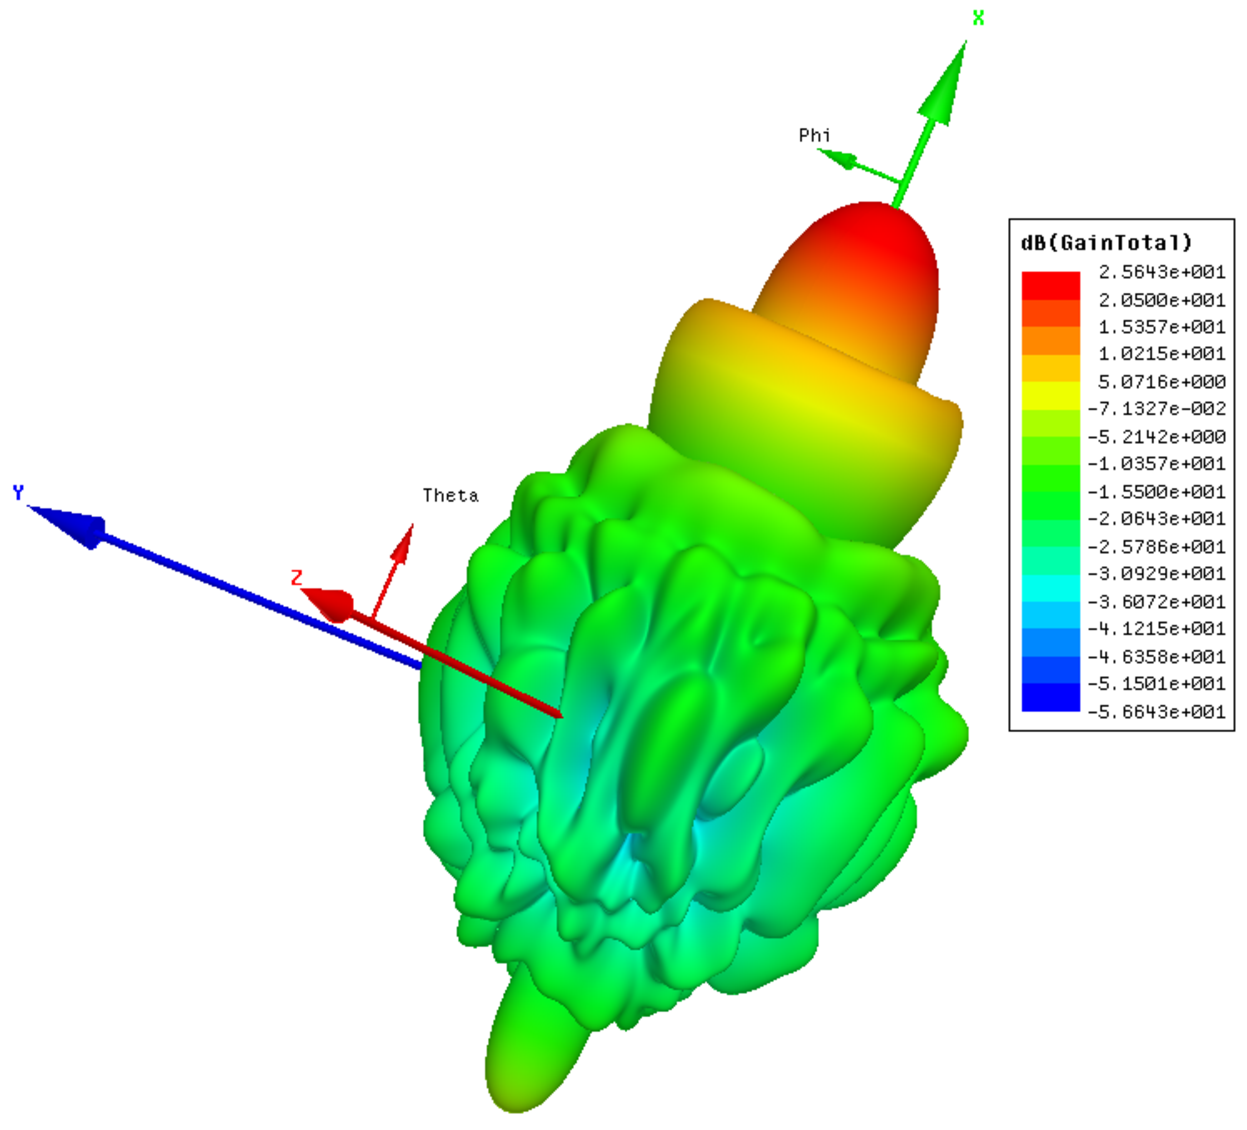
\includegraphics[width=13.4cm]{CircHornRadHFSS}
\caption{Radiation solid at 22~GHz computed with HFSS.}
\label{fig:CircHornRadHFSS}
\end{figure}

\begin{figure}[h!]
\centering
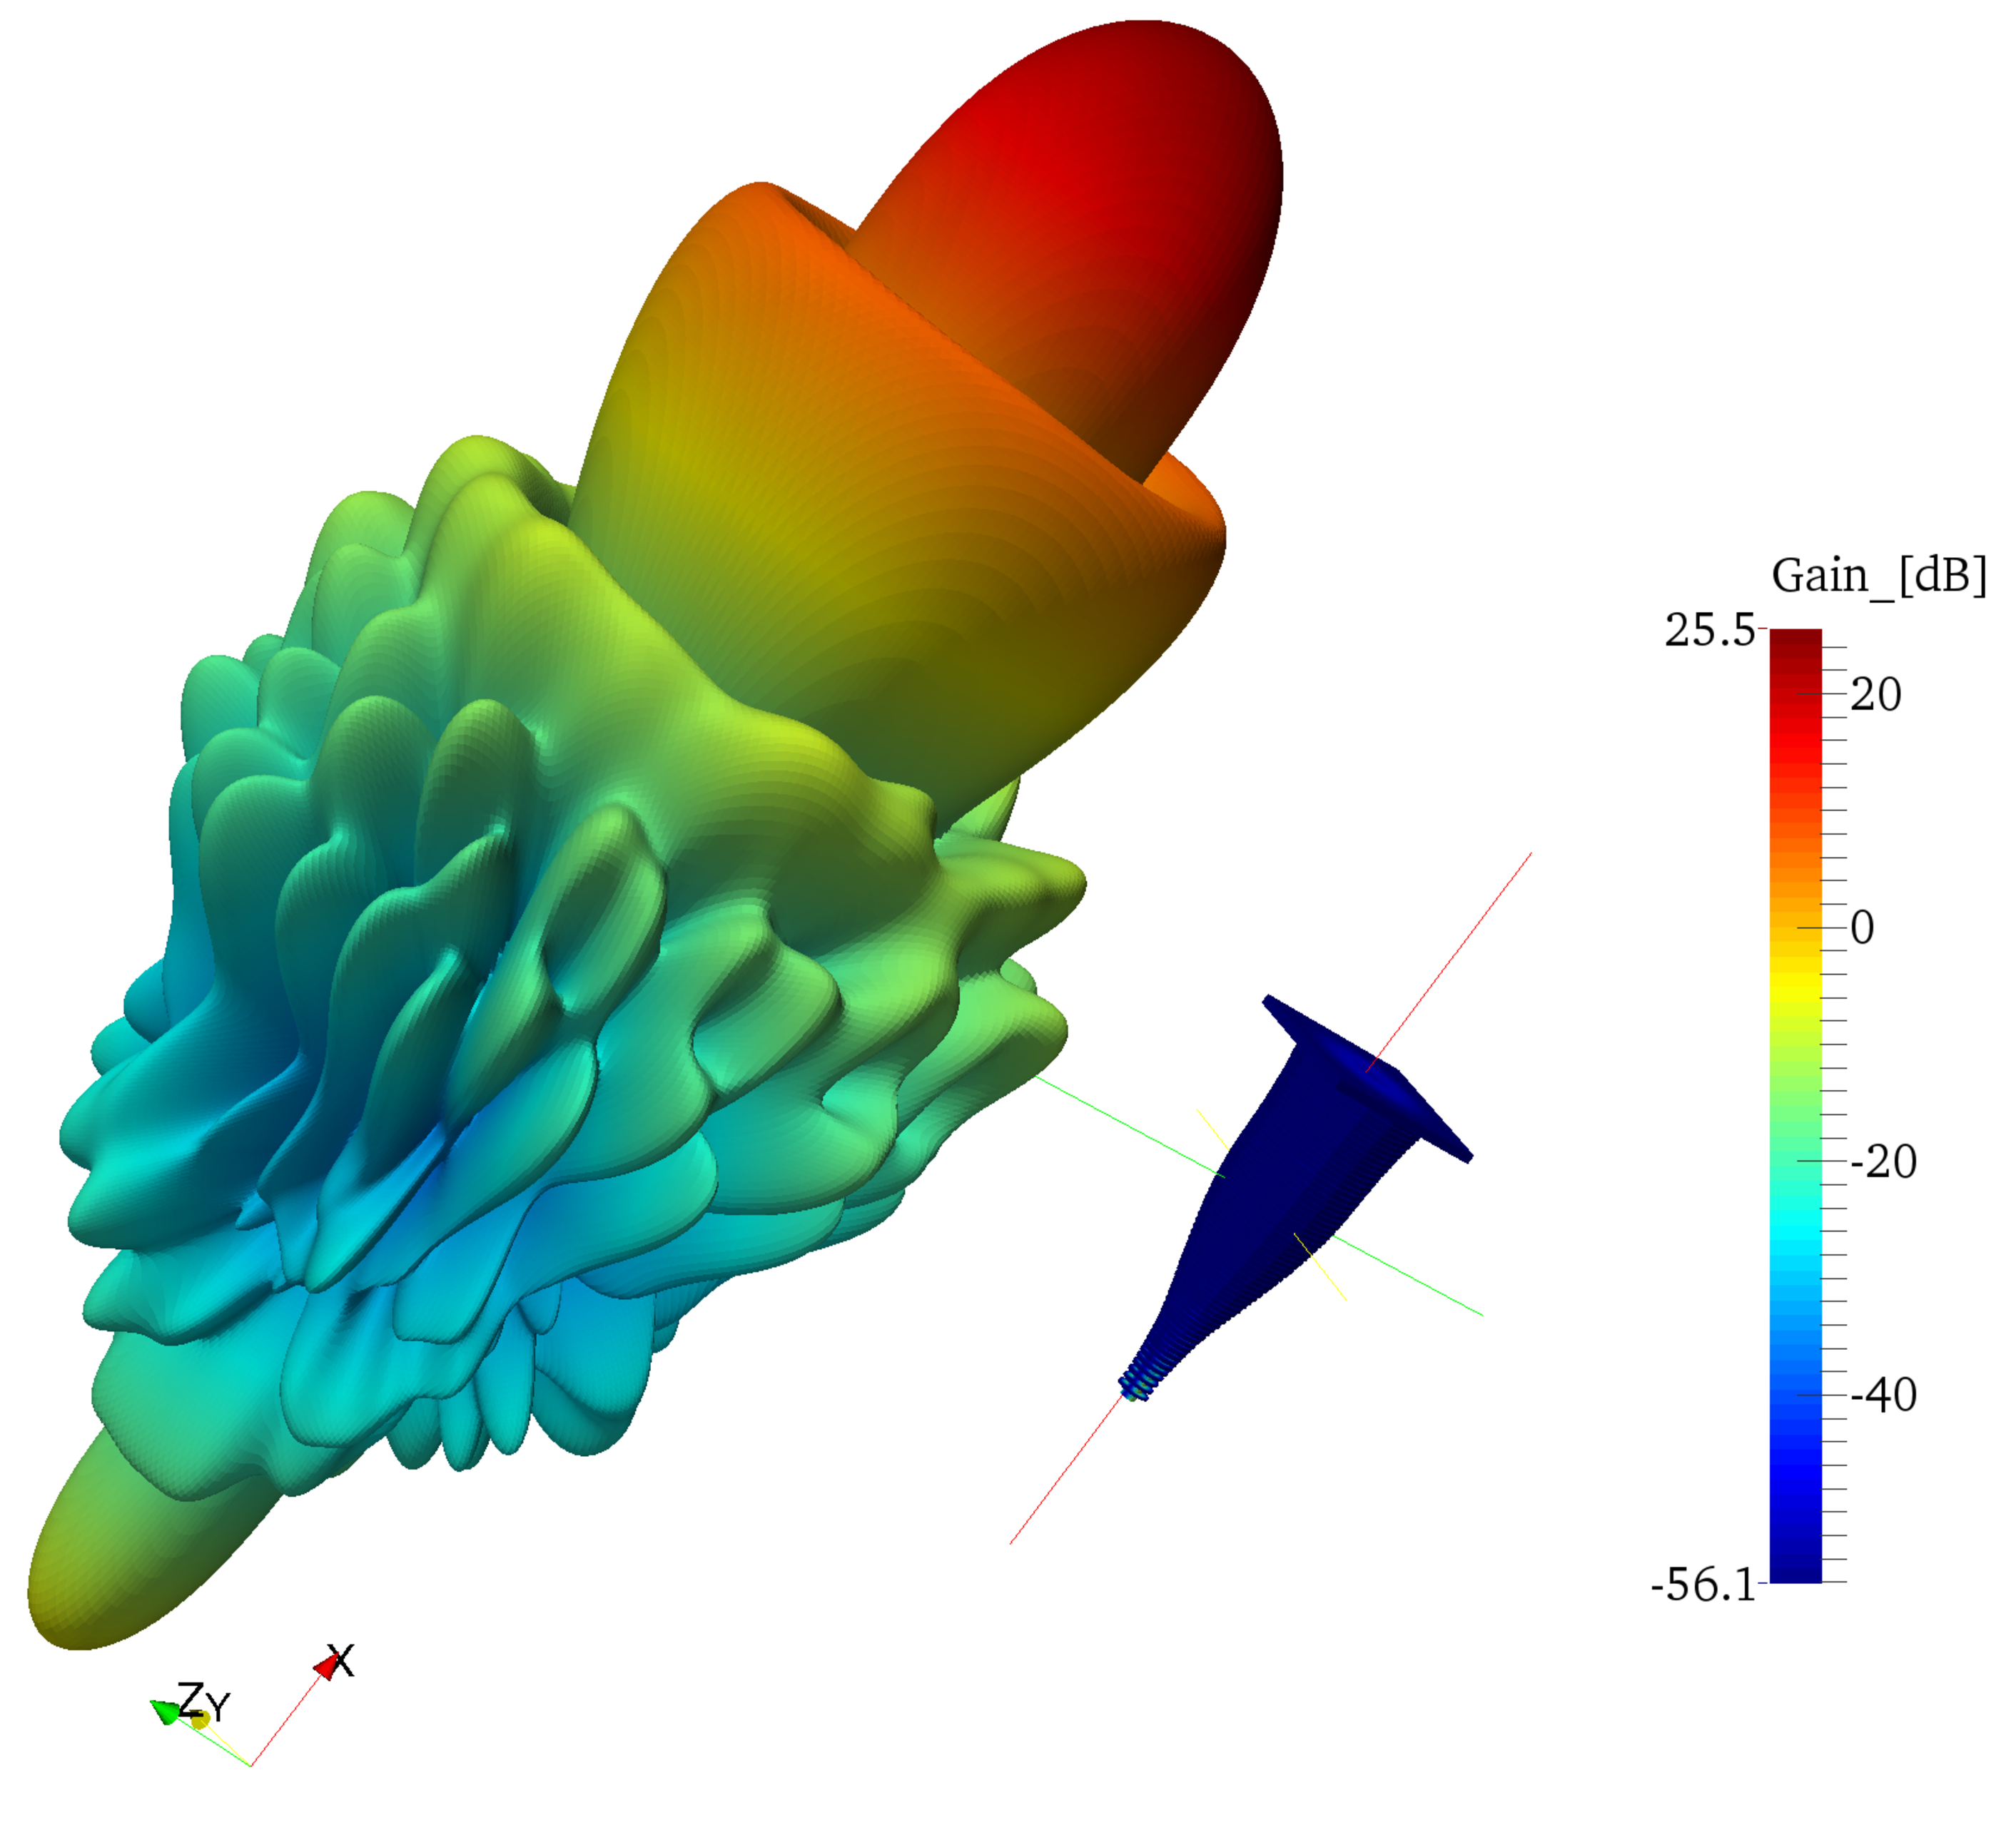
\includegraphics[width=12.4cm]{CircHornRad}
\caption{Radiation solid at 22~GHz computed with FES.}
\label{fig:CircHornRad}
\end{figure}

\begin{figure}[h!]
\centering
\begin{minipage}{6.5cm}
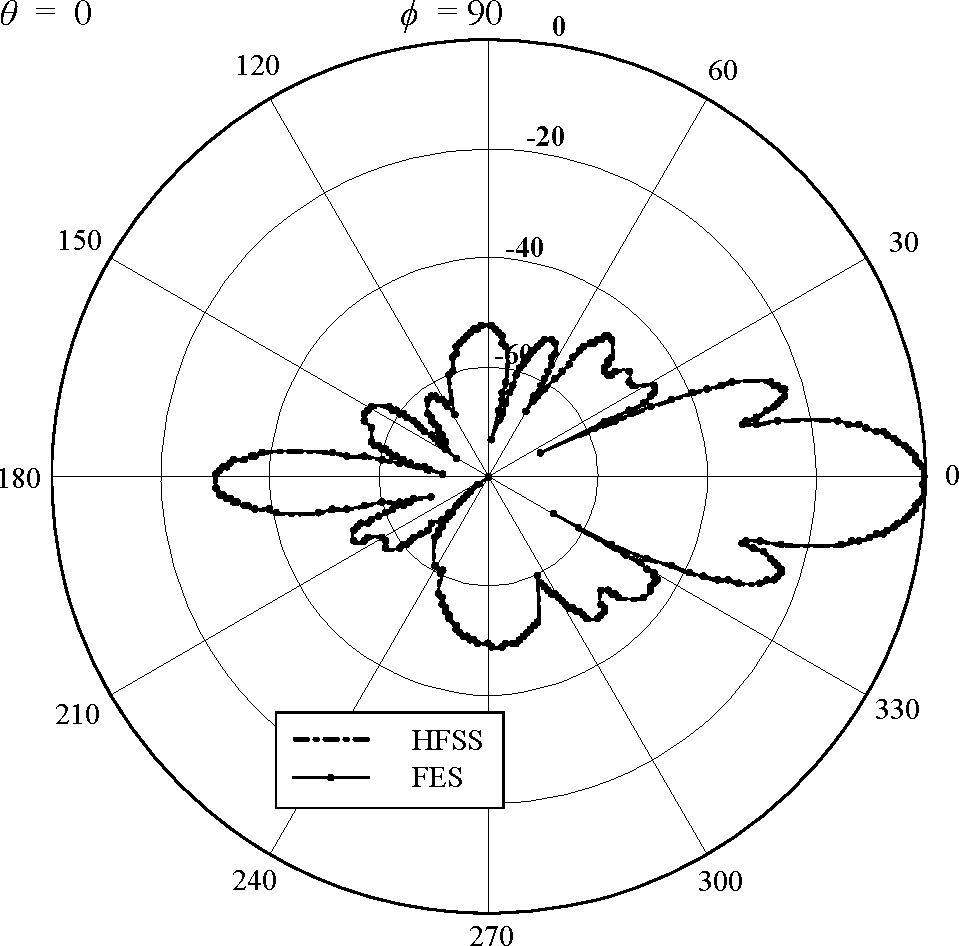
\includegraphics[width=6.4cm]{Polar2}
\end{minipage}
\
\begin{minipage}{6.5cm}
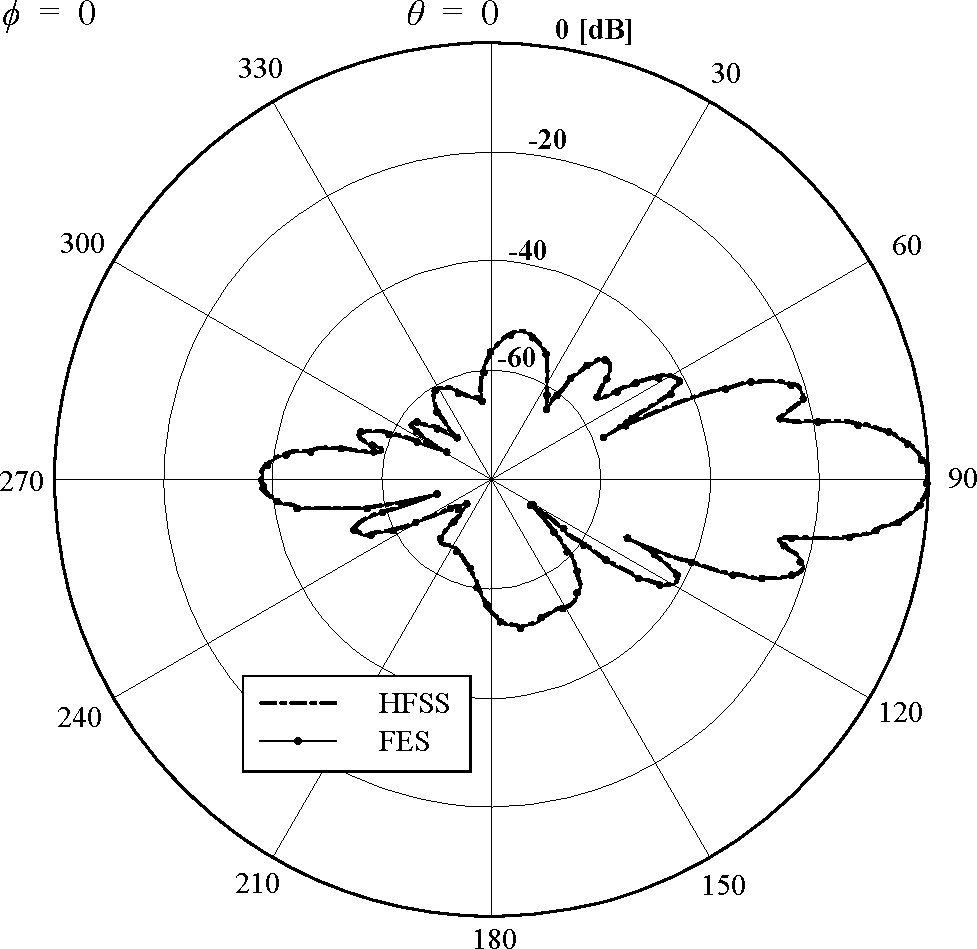
\includegraphics[width=6.4cm]{Polar1}
\end{minipage}
\caption{Normalized gain patterns on the \textit{XY} (left) and the \textit{XZ} (right) planes.}
\label{fig:Polar}
\end{figure}

%\begin{figure}[h!]
%\centering
%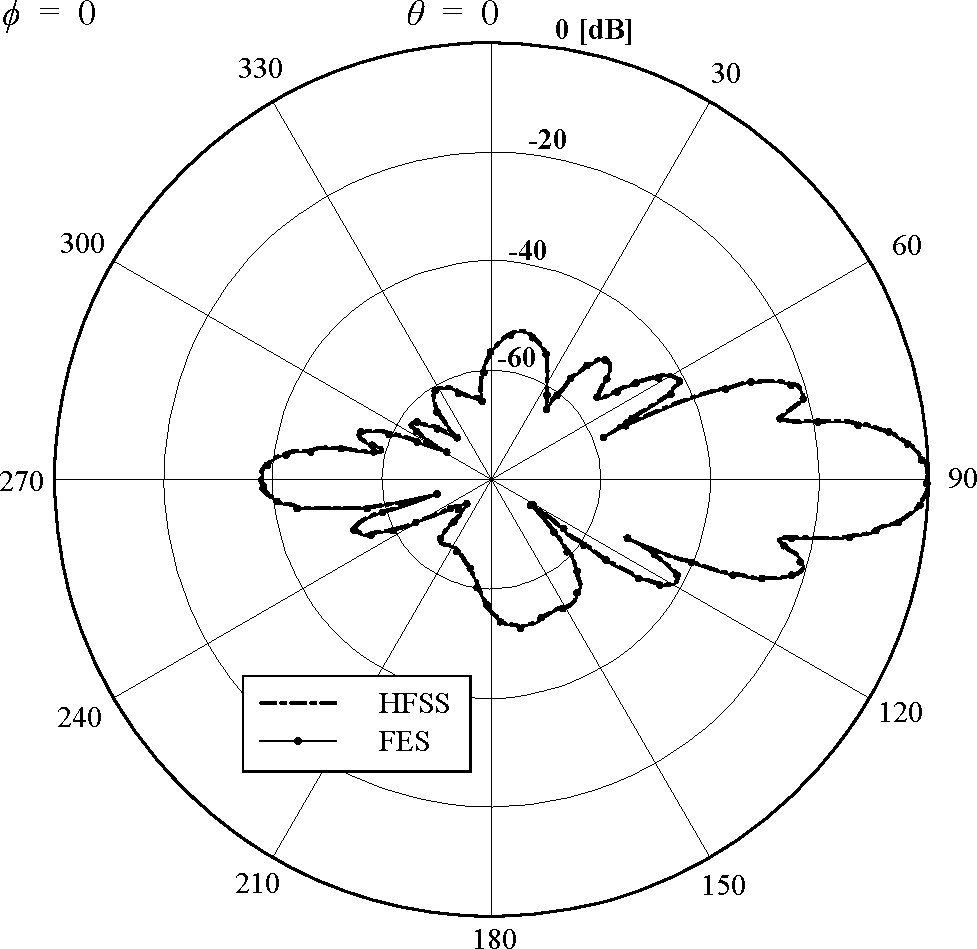
\includegraphics[width=10cm]{Polar1}
%\caption{Normalized gain patterns on the $XZ$ plane comparisons.}
%\label{fig:Polar1}
%\end{figure}


%\subsection{2.4GHz Circular polarization patch antenna analysis}
%
%
%\begin{figure}[ht!]
%\centering
%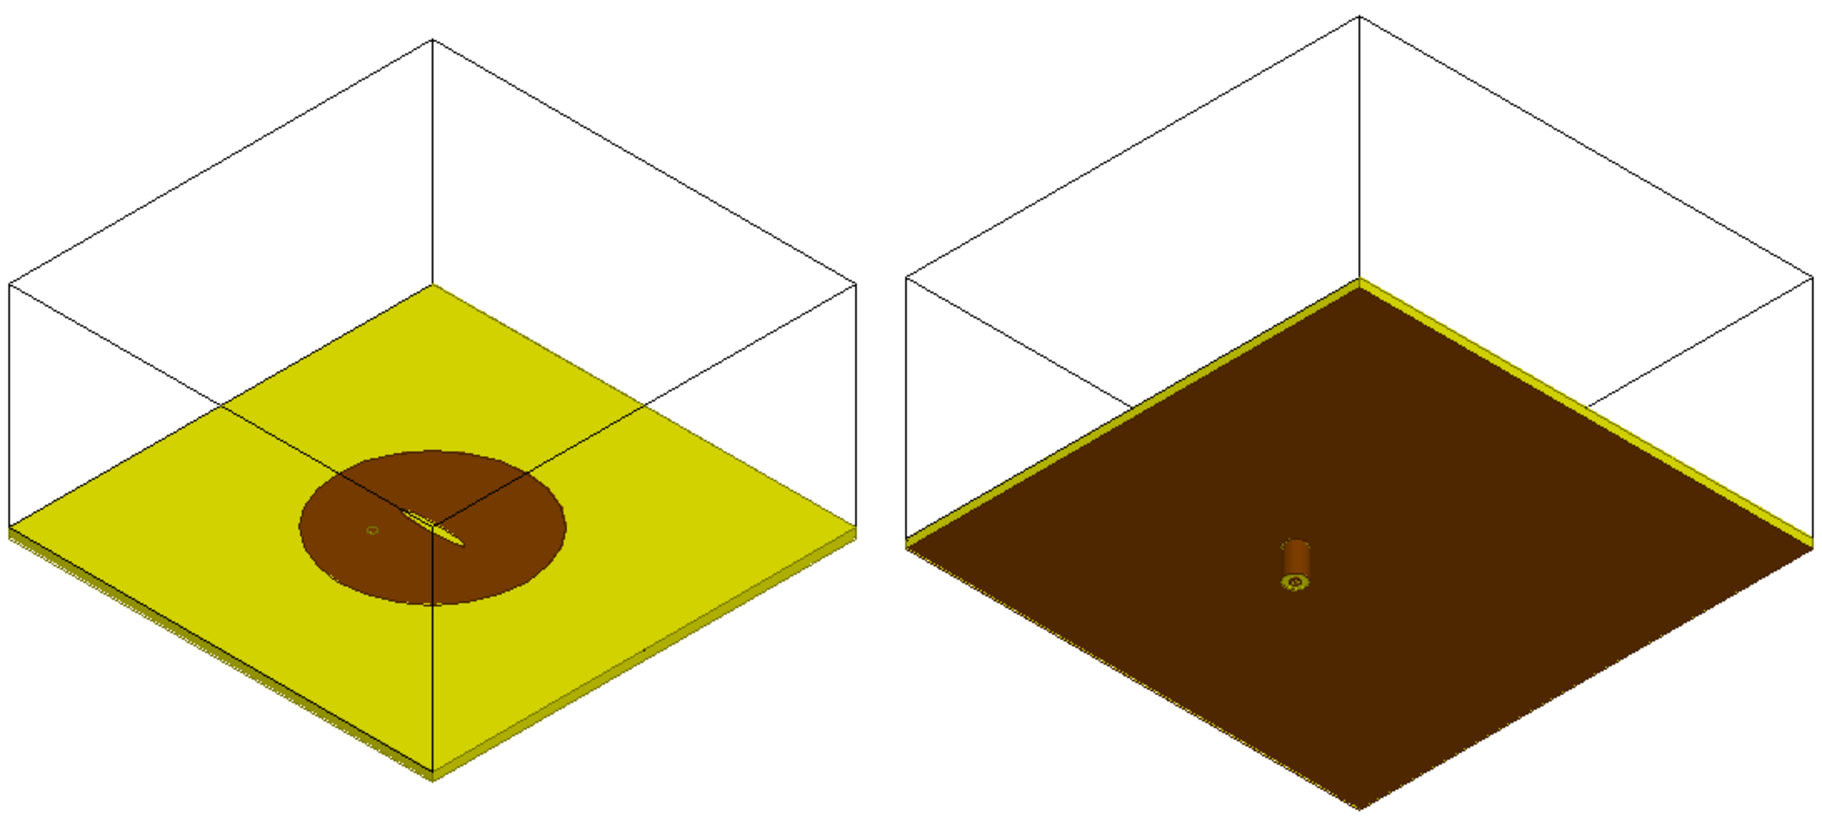
\includegraphics[width=13.4cm]{PatchAntenna}
%\caption{Sketch for the waveguide filter of.}
%\label{fig:PatchAntenna}
%\end{figure}

\clearpage
\subsection{Perfect electric scattering sphere}

Another test, which is \quotes{classical} among all the electromagnetic problems as it founds since more than a century an analytical solution, is that of a metallic sphere located in free-space, made of perfect electric conductor, on which impinges a plane wave from one direction. The domain of finite element analysis is shown in Fig. \ref{fig:Sphere}.

\begin{figure}[ht!]
\centering
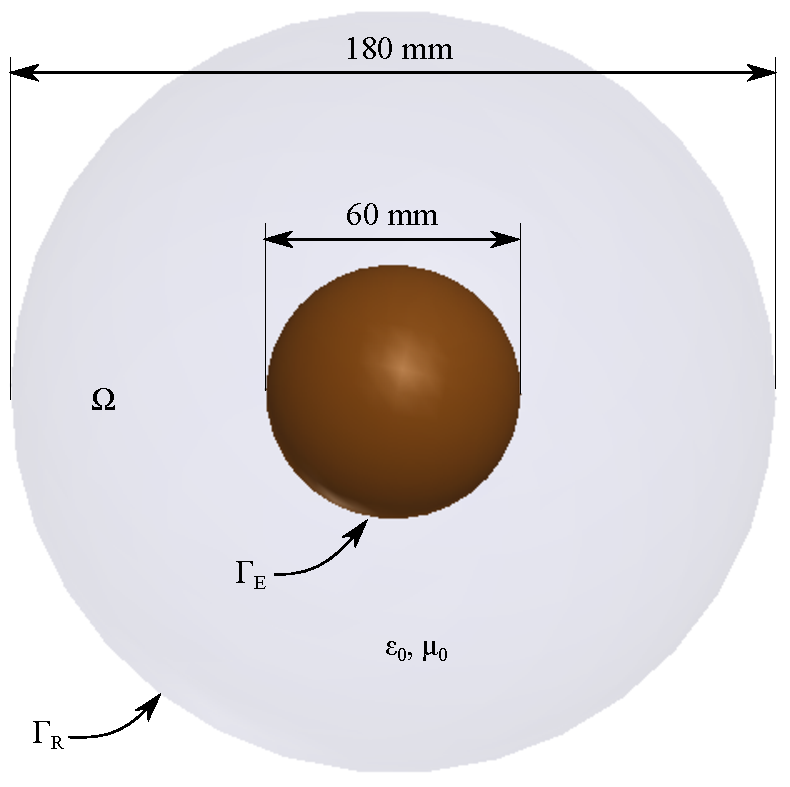
\includegraphics[width=9cm]{Sphere}
\caption{Sketch the scattering problem by a perfectly conducting metallic sphere.}
\label{fig:Sphere}
\end{figure}

Consider a plane wave at frequency $f$, traveling in free-space in the direction $\hat{\mathbf{z}}$. Hence the incident electric field, polarized along $\hat{\mathbf{x}}$, can be written as

$$\mathbf{E}^{inc} = | \mathbf{E}^{inc}| \exp{-jk_0 \hat{\mathbf{z}} \cdot \mathbf{r} } \ \hat{\mathbf{x}},$$

\noindent and the magnetic field

$$\mathbf{H}^{inc} = \frac{1}{\zeta_0} \mathbf{E}^{inc} \times \hat{\mathbf{z}} =  \frac{1}{\zeta_0}| \mathbf{E}^{inc}| \exp{-jk_0 \hat{\mathbf{z}} \cdot \mathbf{r} } \ \hat{\mathbf{y}}.$$

These values can be substituted in the formulation \ref{eq:FEMformScatt} in order to compute the integrals on $\Gamma_R$. In this test case, we have considered the wave, with $| \mathbf{E}^{inc}| = \frac{\mathrm{V}}{\mathrm{m}}$, to be oscillating at 6~GHz. The mesh of 73,252 tetrahedra led to only 89,946 unknowns. The electric fields computed by both HFSS and FES (double precision) are shown in Figs \ref{fig:SphereHFSS} and \ref{fig:SphereField}, considering first order basis functions. The maximum magnitude of the electric field in the domain of analysis $\Omega$ was of about $1.52~\frac{\mathrm{V}}{\mathrm{m}}$ in both cases, and the overall distribution was approximately the same. Due to linear polarization along the $\hat{\mathbf{x}}$ axis, the $XZ$ cut-plane, so-called \textit{E}-plane, shows a different electric field distribution respectively to that on the $YZ$ cut-plane, the \textit{H}-plane.

\begin{figure}[ht!]
\centering
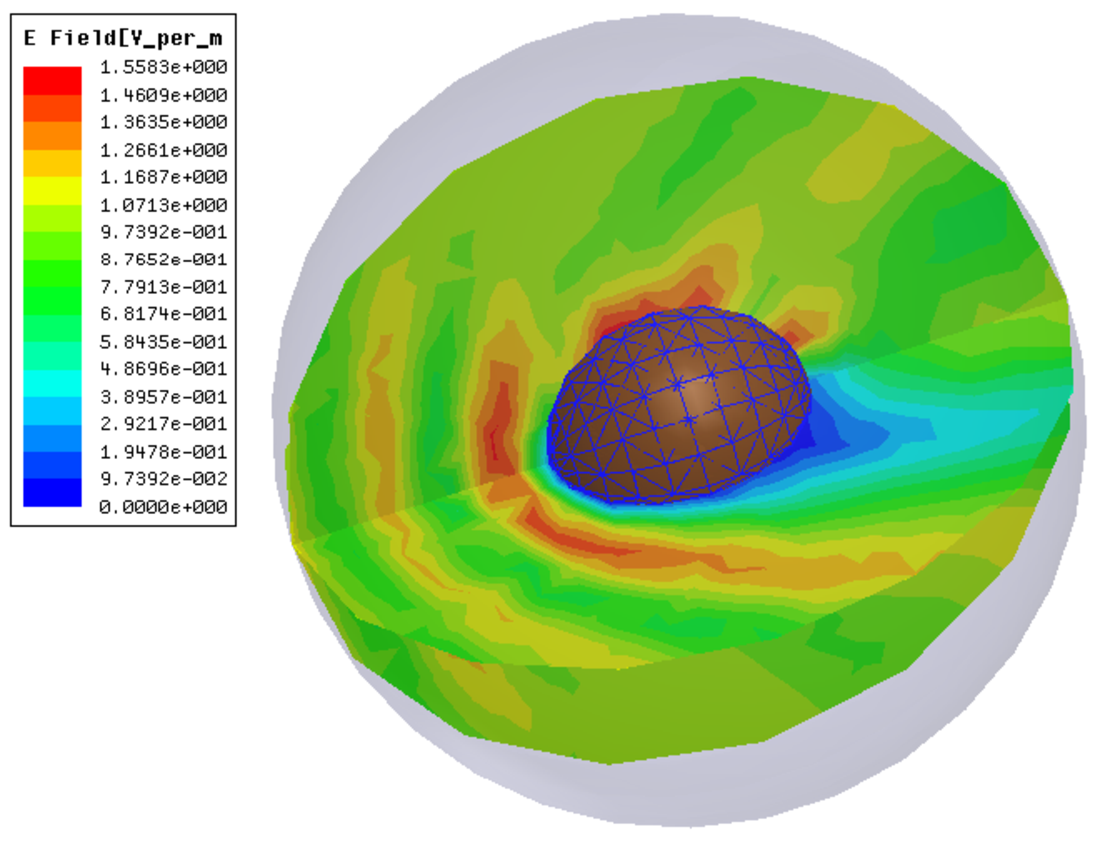
\includegraphics[width=10cm]{SphereHFSS}
\caption{Electric field surrounding the perfectly conducting metallic sphere, computed with HFSS.}
\label{fig:SphereHFSS}
\end{figure}
\begin{figure}[ht!]
\centering
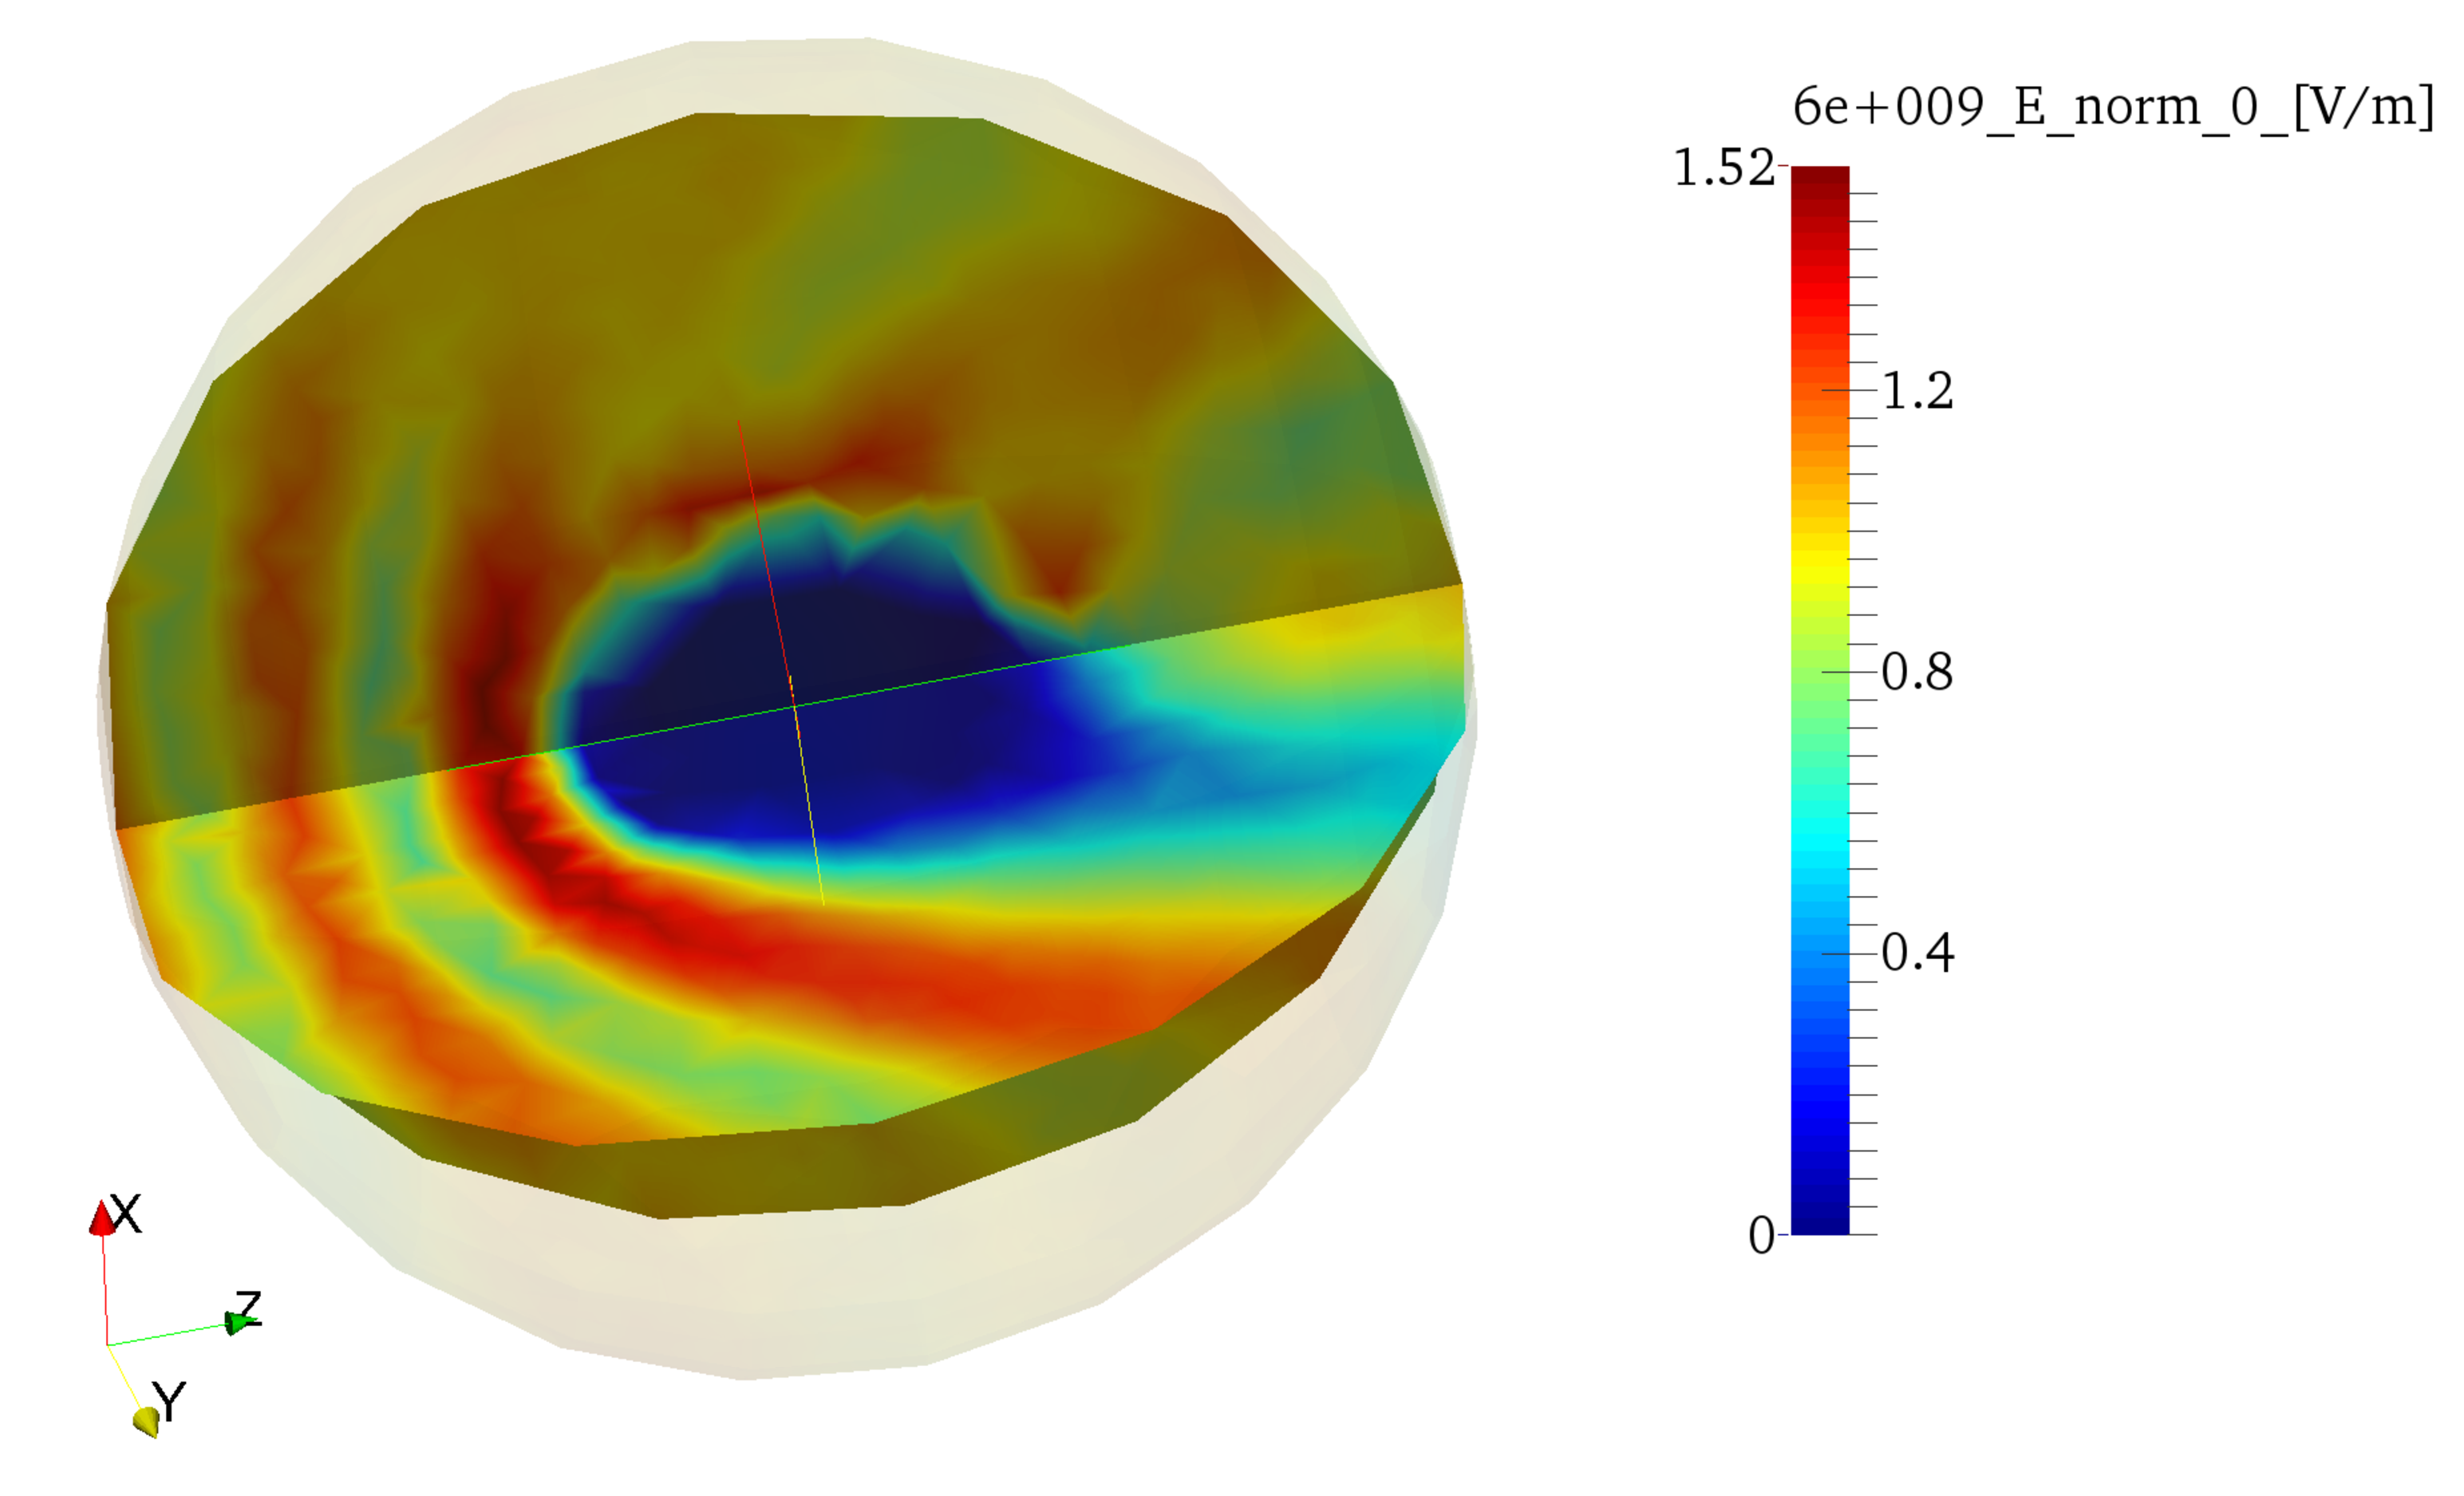
\includegraphics[width=13cm]{SphereField}
\caption{Electric field surrounding the perfectly conducting metallic sphere, computed with FES.}
\label{fig:SphereField}
\end{figure}

The radar cross section magnitude in decibels is shown in Figs. \ref{fig:SphereRCSHFSS} and \ref{fig:SphereRCS}. Also here there is a good a agreement between the solvers, and a maximum of -12~dB in the $\hat{\mathbf{z}}$ direction. The mean relative error between the single precision and HFSS is of $4.49\times 10^{-4}$ while with the double precision solver we had $9.21\times 10^{-5}$, hence the difference in the formulations is more important. However, in practical analyzes, one may consider the results equivalent ($1\%$ error is still neglectable).

\begin{figure}[h]
\centering
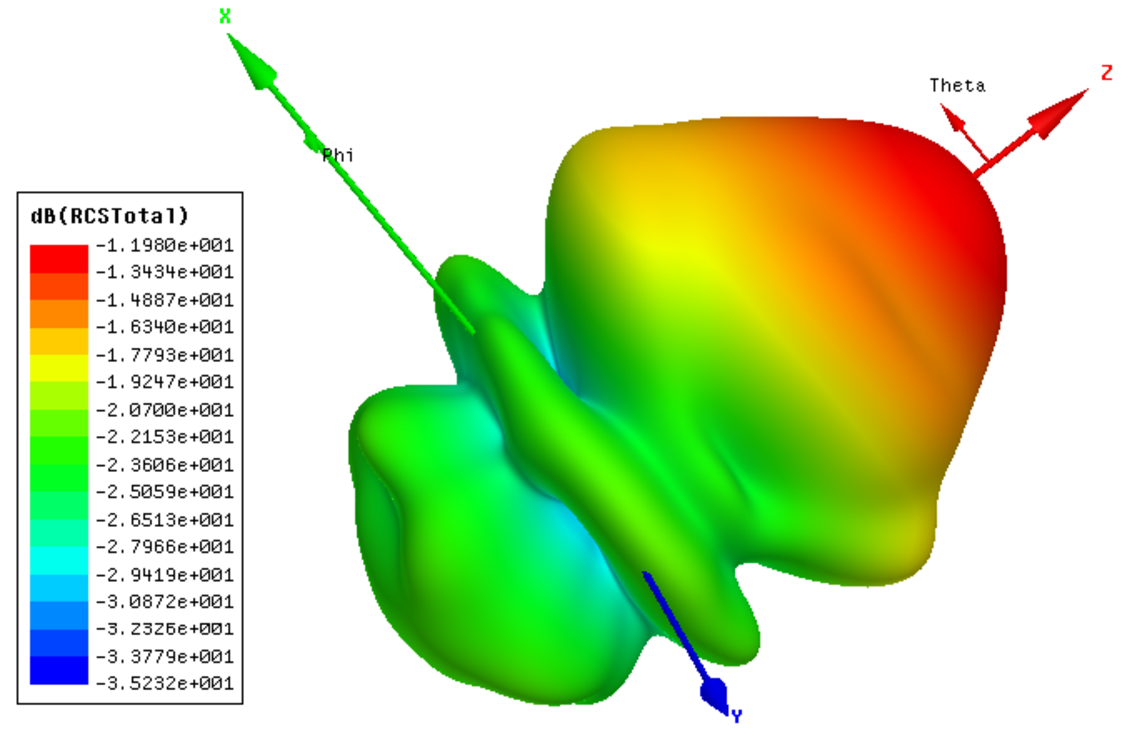
\includegraphics[width=12.4cm]{SphereRCSHFSS}
\caption{Radar cross section of the sphere, computed with HFSS.}
\label{fig:SphereRCSHFSS}
\end{figure}

\begin{figure}[h]
\centering
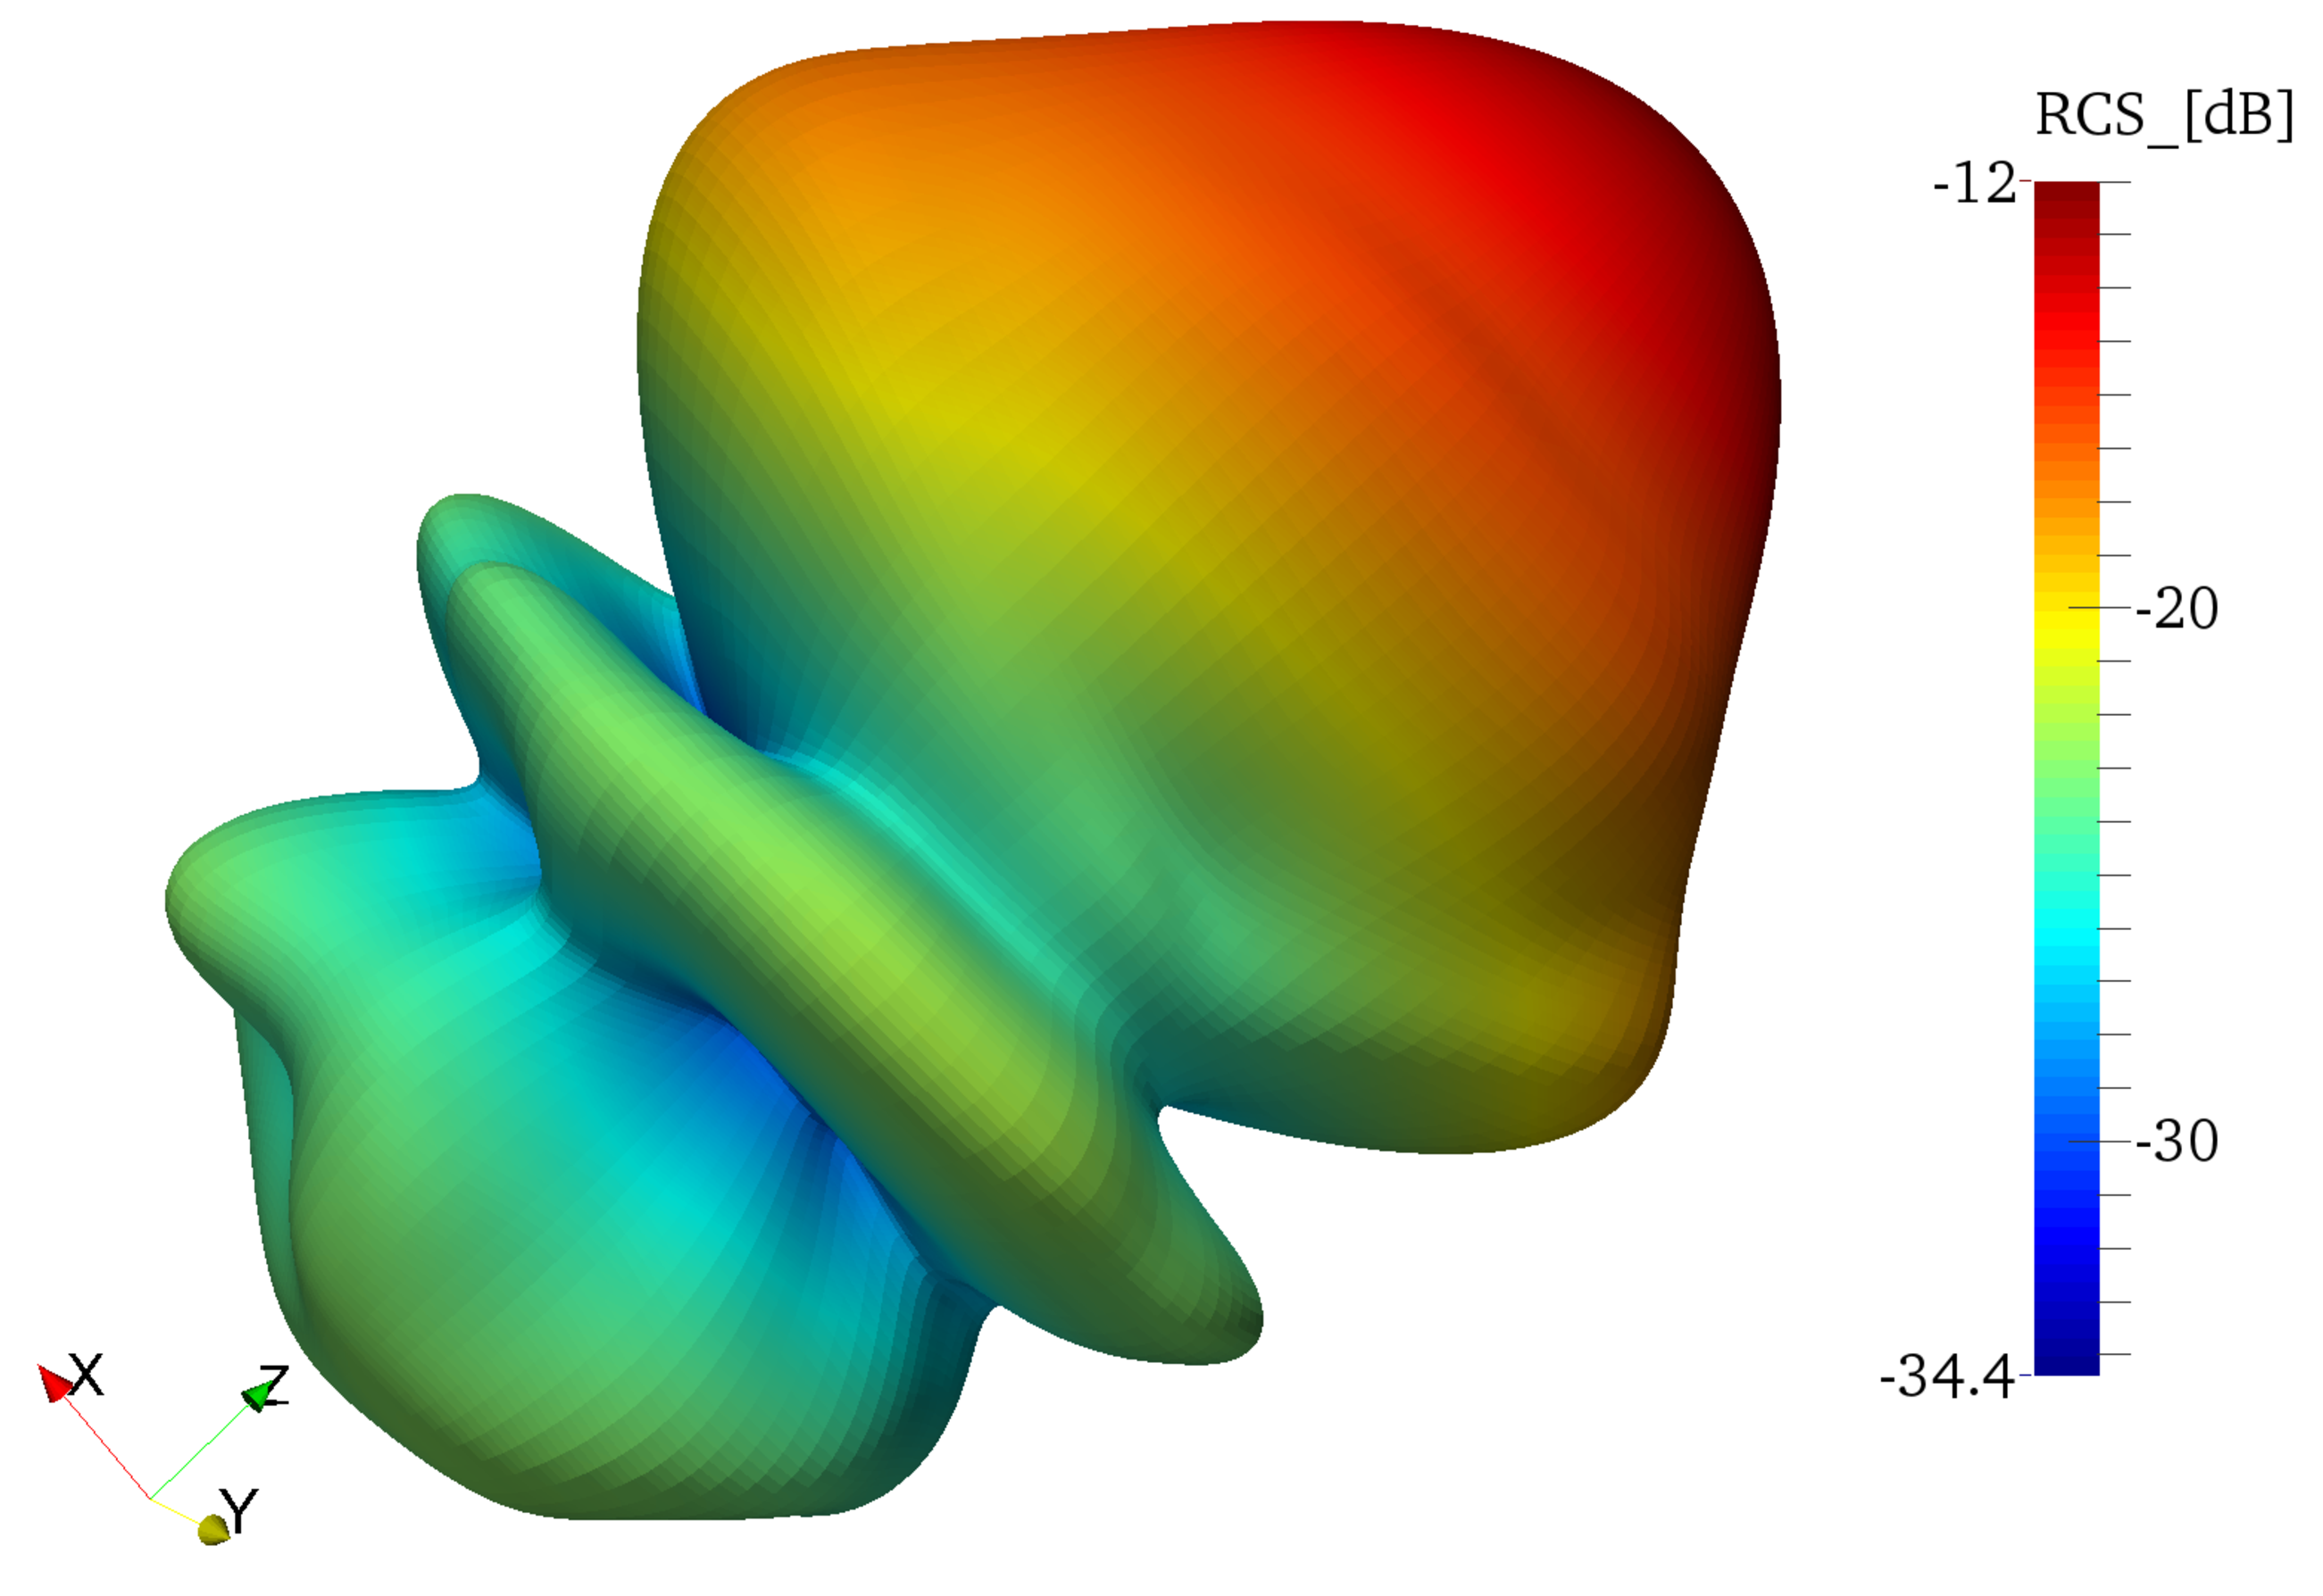
\includegraphics[width=11cm]{SphereRCS}
\caption{Radar cross section of the sphere, computed with FES.}
\label{fig:SphereRCS}
\end{figure}
\clearpage
As said previously, in Paraview it is possible to visualize the electric far field vectors (in the limit of $r\rightarrow \infty$), and hence its polarization. In Fig. \ref{fig:SpherePol}, these vectors are shown and one can see that the fields scattered in $\hat{\mathbf{z}}$-direction remain polarized as the impinging wave, while in other directions the fields might change their polarization.

\begin{figure}[h]
\centering
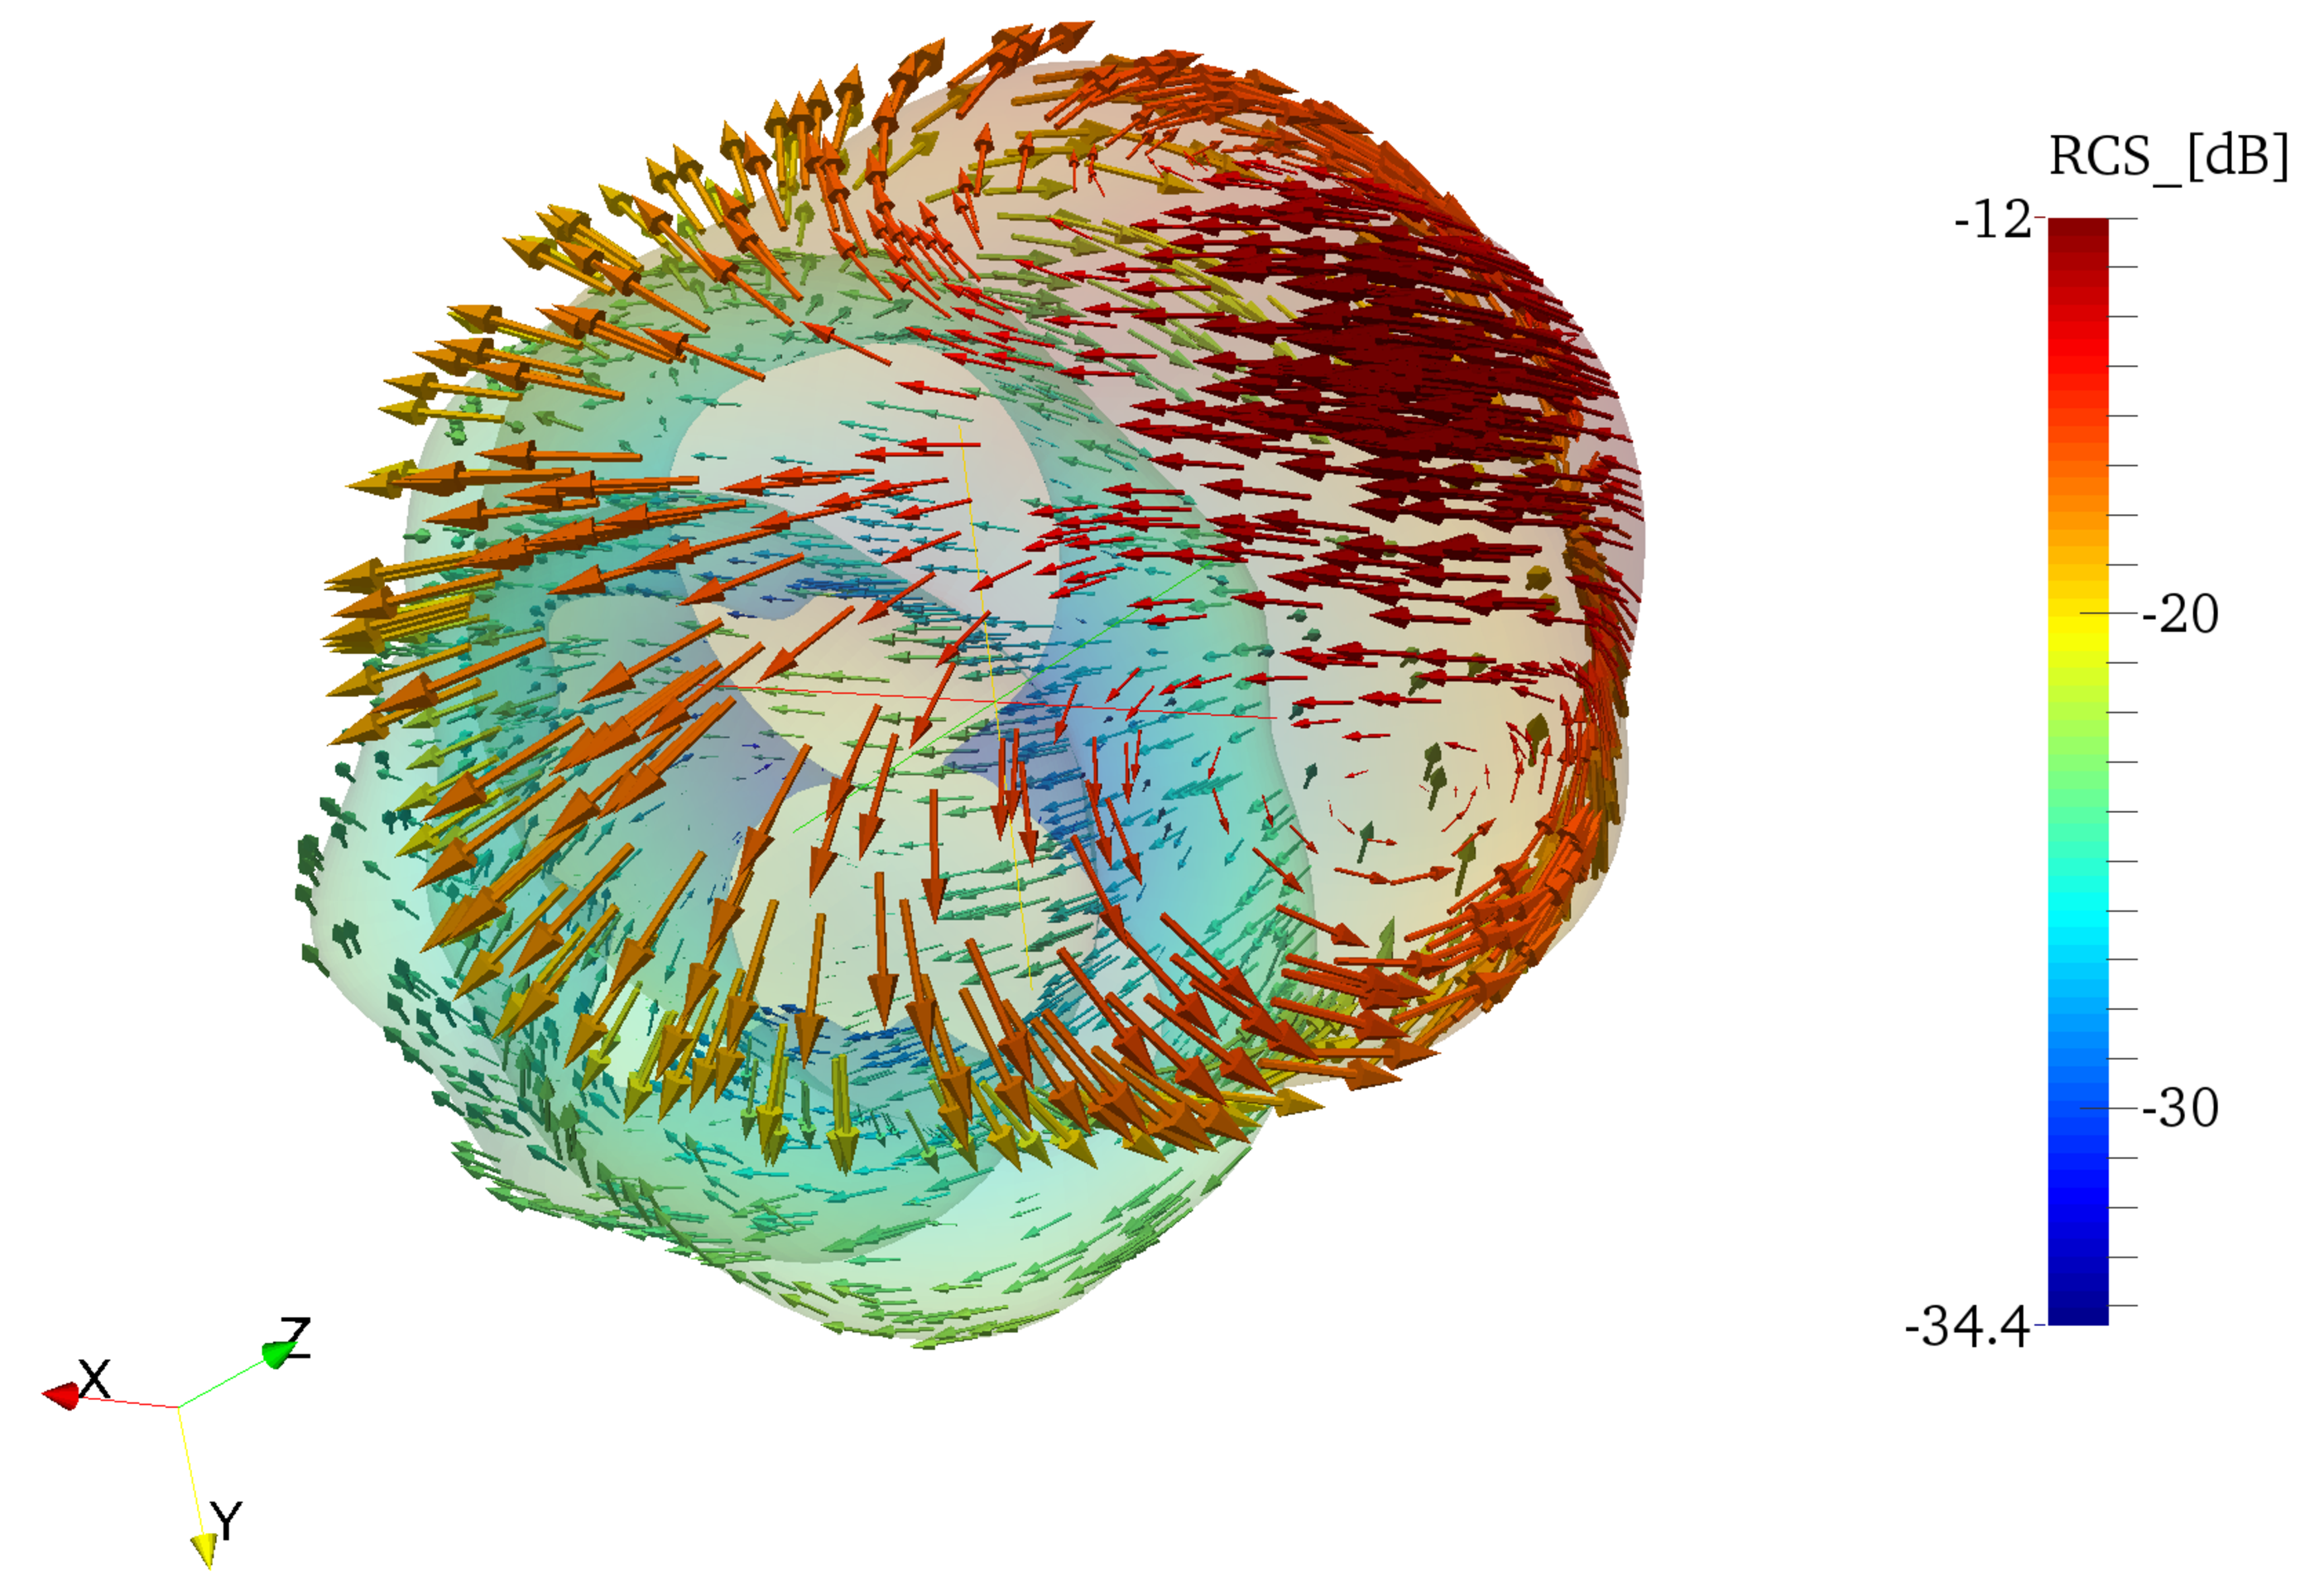
\includegraphics[width=12cm]{SpherePol}
\caption{Polarization of the electric far field visualized with Paraview.}
\label{fig:SpherePol}
\end{figure}
\thispagestyle{empty}
\cleardoublepage
% !TEX root = ln_diss.tex
\graphicspath{{img/ch2/}}
\chapter[Domain decomposition methods]{Domain decomposition methods for large  problems} \label{chap:DD}

The most important limit of numerical full-wave electromagnetic analyzes is the fact computational resources are limited, at least when trying to fit all the problem in memory at a time. Even if one had infinite computational resources, many algorithms, say even the solvers, would be such that it would require a huge amount of times to solve very large problems. 

Nowadays, we refer to \quotes{large problems} to meshes that lead to millions of unknowns, up to several tens of millions. In chapter \ref{chap:FE}, we could solve acceptably a 600,000 unknowns problem in about 2 minutes (section \ref{sec:Horn}). But notice that it required about 3.1~GB of memory, which can easily fit in modern (low-cost) personal computers. But what would happen if we try to analyze an array of this antenna? The problem, if full-wave solution is still sought for, would be to solve the wave equation in the all the horns connected by a wide radiation bounding box, allowing thus to consider mutual couplings between the antennas. This slightly increases the number of the finite element unknowns that we would have upon multiplying the 600,000 unknowns by the number of antennas. It is evident that we quickly reach the limit on a simple computer. To overcome this problem, parallel processing needs to be considered, devoting the matrix inversion to multiple computers (increasing in such a way the overall physical memory) interconnected through a high speed network. With iterative solvers, even if they require a minimum of memory which is necessary to store the built finite element system, the number of iterations might dramatically grow with the number of unknowns, hence the amount of times required for an acceptable analysis might not be tolerable.

Among the methods developed to increase the computational efficiency of finite element solvers, domain decomposition (DD) methods have found noticeable interest in the last decade.  They allow to analyze a whole problem upon partitioning it and computing solutions for each smaller problem. Then, all the solutions are \quotes{connected} in order to recover the effective solution within the whole domain. Relying on a \textit{divide et impera} scheme, these methods are \textit{de facto} intrinsically parallelizable. In fact, multiple domains can be analyzed contemporaneously on different processors. Another interesting aspect is that, when no cluster of computers is available to scale the problem, each smaller problem or \textit{subdomain} can be tackled faster with direct solvers, one at a time, while keeping in memory only the necessary information to recover the global solution. 

A critical part of the domain decomposition method is how the information on the subdomains is collected and transferred to the global problem in order to achieve the original problem solution. There exist in literature \cite{toselli2005domain, mathew2008domain} many mathematically proven algorithms that lead to a domain decomposed solution for a variety of problems (Laplace, Helmholtz, Navier-Stokes and other PDEs) given a particular decomposition scheme. The first domain decomposition algorithm is more than a century old: Schwarz proposed, at the end of $19^\mathrm{th}$ century, an alternating algorithm for the solution of Poisson problems on overlapping subdomains \cite{schwarz1972gesammelte}, proving later its convergence. With the advent of the personal computer, this research field begun to find many interesting applications. The first non-overlapping appeared in 1990 \cite{lions1990schwarz} and this opened the investigation to a new class of domain decomposition algorithms. It is evident, from a computational point of view, how this decomposition scheme is easier to handle. However, new truncation conditions have to be enforced as only the informations on the boundaries can be transferred to the adjacent subdomains.

\begin{figure}[ht!]
\centering
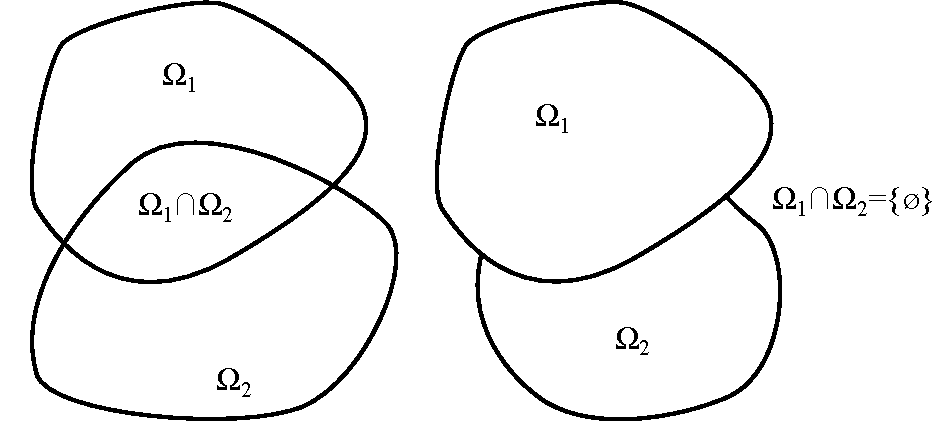
\includegraphics[width=10cm]{DDnonoverlaping}
\caption{Overlaping and non-overlaping domain decomposition schemes.}
\label{fig:DDnonoverlaping}
\end{figure}

In this chapter, we investigate two non-overlapping or \textit{iterative substructuring} domain decomposition methods: a Schur Complement based method and a Finite Element Tearing and Interconnecting Dual-Primal (FETI-DP) based method in order to solve large radiation problems either for sequential or parallel computing. In particular, the DD frameworks are employed as preconditionners for iterative solvers for sequential processing. Direct solvers, being the best suited for small problems, can be employed in a DD framework to accelerate the convergence of iterative solvers. Several tests will be performed, first analyzing the performances of the algorithms on an arbitrarily partitioned rectangular waveguide problem.

\section{Schur complement based domain decomposition}\label{sec:SchurDD}

As we have seen in chapter \ref{chap:FE}, the unknowns resulting from a Galerkin framework are somehow related to mesh entities. If one could collect sequentially, during the mapping to the system matrix, the unknowns pertaining to a subdomain, then the resulting matrix would have a block-diagonal form. Of course, the unknowns related to the subdomain boundaries cannot be duplicated, otherwise the resulting system would be undetermined. Thus, one can collect all the unknowns pertaining to the boundaries between subdomains in a new diagonal block. These unknowns, being dependent on the elements pertaining to two (or more) adjacent subdomains, will lead to global matrix entries connected to these subdomains unknowns apart from diagonal blocks.

\begin{figure}[ht!]
\centering
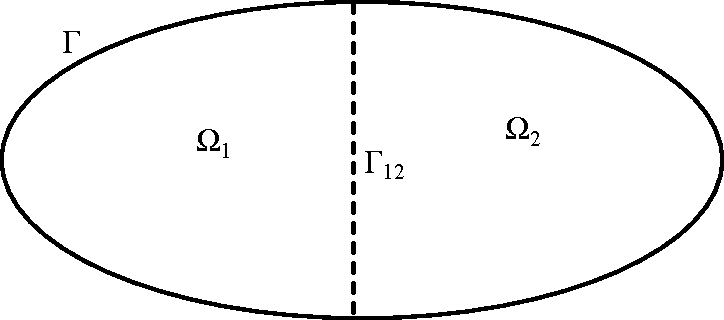
\includegraphics[width=8cm]{DDSchur2}
\caption{Schur complement based domain decomposition sketch for two subdomains.}
\label{fig:DDSchur2}
\end{figure}

Consider the domain decomposition of $\Omega$ in two subdomains as shown in Fig. \ref{fig:DDSchur2}. The resulting system matrix of any formulation employed in chapter \ref{chap:FE} is

\begin{equation}
\label{eq:DDSchurFull}
\begin{bmatrix}
A_{\Gamma\Gamma} & A_{\Gamma1} & A_{\Gamma2}\\
A_{1\Gamma} & A_{11} & \\
A_{2\Gamma} &  & A_{22}
\end{bmatrix}
\begin{bmatrix}
x_{\Gamma}\\
x_{1}\\
x_{2}
\end{bmatrix}
=
\begin{bmatrix}
B_{\Gamma}\\
\phantom{B}\\
\phantom{B}
\end{bmatrix},
\end{equation}

\noindent where the subscript $\Gamma$ refers to shape functions with related mesh entity on $\Gamma \equiv \Gamma_E \cup \Gamma_H \cup \Gamma_R \cup \Gamma_{WG} \cup \Gamma_{12}$, and the subscript $j \in \lbrace 1,2 \rbrace$ refers to unknowns pertaining exclusively to mesh entities in $\Omega_j$. Notice that the right-hand side has only non-zero entries for the formulations employed in chapter \ref{chap:FE}, the Dirichlet boundary conditions corresponding to perfect electric conductors. Furthermore, when isotropic materials are considered (as done almost everywhere throughout this dissertation), the system matrix is symmetric and \eqref{eq:DDSchurFull} can recast in

\begin{equation}
\label{eq:DDSchurSym}
\begin{bmatrix}
A_{\Gamma\Gamma} & A_{\Gamma1} & A_{\Gamma2}\\
A_{\Gamma1}^T & A_{11} & \\
A_{\Gamma2}^T &  & A_{22}
\end{bmatrix}
\begin{bmatrix}
x_{\Gamma}\\
x_{1}\\
x_{2}
\end{bmatrix}
=
\begin{bmatrix}
B_{\Gamma}\\
\phantom{B}\\
\phantom{B}
\end{bmatrix}.
\end{equation}

The system of \eqref{eq:DDSchurSym} can now be solved exploiting the Schur complement concept:

\begin{itemize}
\item Assemble the Schur complement matrix $\mat{S} = \mat{A_{\Gamma\Gamma}} - \sum_{j=1}^2 \mat{A_{\Gamma j}} \mat{A_{jj}}^{-1} \mat{A_{\Gamma j}}^T$ and the relative right-hand side $\mat{G} = \mat{B_{\Gamma}}$,
\item Solve the Schur complement system $\mat{x_\Gamma} = \mat{S}^{-1} \mat{G}$,
\item Recover for the internal unknowns $\mat{x_j} = \mat{A_{jj}}^{-1} (-\mat{A_{\Gamma j}}^T \mat{x_\Gamma})$.
\end{itemize}

In the first step, a matrix denser than the original $\mat{A_{\Gamma\Gamma}}$ is assembled upon adding (as done for the global finite element matrix after the computation of an element matrix) the contributions of each subdomain. This requires the computation of $\mat{A_{jj}}^{-1}$ (intrinsically dense), which itself can be handled easily with sparse direct solvers (and exploiting symmetries in this case), however, the computation of the matrix-matrix product $\mat{A_{jj}}^{-1} \mat{A_{\Gamma j}}^T$ may lead to a memory consuming result. Hence, one should consider making the most of $\mat{A_{\Gamma j}}^T$ sparsity to reduce the resulting rectangular matrix, avoiding to save into memory its null column vectors.

The second step corresponds to the inversion of a dense $\mat{S}$ matrix. As it is known, this operation has an asymptotic complexity of $O(N_\Gamma^3)$, which indeed increases as the number of subdomains is increased. In fact, the unknowns on the boundary between subdomains increases. One may solve the problem on boundaries with a Krylov subspace iterative solver, preconditioning it with a \textit{thresholded incomplete LU} factorization  \cite{saad1994ilut} or the \textit{incomplete Cholesky} factorization which takes the advantage of matrix symmetry. In fact, it has been proved \cite{mathew2008domain} that if the original system is symmetric, then the Schur complement matrix will also be symmetric.

The last step requires subdomains matrices inversion. These can be stored in memory (non-volatile preferably) during the first step where they were also used. An additional matrix-vector product has to be computed.

The resulting concatenated solution vector $\vect{x}_\mathrm{Schur} = \vect{x_\Gamma \ x_1 \ x_2}^T$ is equal, within numerical error, to that of the direct solution of the whole system in \eqref{eq:DDSchurSym} when direct or iterative solvers are ran up to numerical precision. Furthermore, the parallelization internal to the first and the last steps is immediate.

In our treatment, several critical points have emerged from the use the Schur complement method, when looking forward to analyze large problems

\begin{itemize}
\item The assembly of the Schur complement matrix requires the computation of large rectangular matrices $\mat{A_{jj}}^{-1} \mat{A_{\Gamma j}}^T$. One may assemble the whole Schur complement to domain $\Omega_j$, $\mat{A_{\Gamma j}} \mat{A_{jj}}^{-1} \mat{A_{\Gamma j}}^T$, upon exploiting the sparsity of $\mat{A_{\Gamma j}}^T$ and considering a few columns at a time in order to reduce the overall memory fill-in. However, if the number of unknowns pertaining to $\Omega_j$ is very large, then this step might result to be excessively time demanding.
\item The overall Schur complement matrix $\mat{S}$ is dense, and the complexity of its inversion grows dramatically with the boundary unknowns, and, consequently, with the number of subdomains.
\end{itemize}

\noindent Both the previous points are in contrast: if one tries to alleviate the computation of the Schur complement matrices to each subdomain by increasing the number of subdomains (hence reducing the related domain unknowns number), then the inversion of the overall Schur complement matrix results hampered by an increase of the boundary unknowns and \textit{viceversa}. This has led to the research of an appropriate Schur complement based domain decomposition preconditionner to be used in an iterative solver for the whole problem \eqref{eq:DDSchurSym}.

In contrast with the method that will be introduced in the next section, Schur complement based methods are referred to as \quotes{primal} iterative substructuring methods in the way they employ only functions in the space of the unknown global function to enforce the continuity between subdomains. For instance, continuity between the subspaces spanned in each subdomain without its boundaries is enforced by a discrete version of the Steklov-Poicar\'e operator or \quotes{Dirichlet-to-Neumann} map \cite{mathew2008domain}, the Schur complement matrix, serving as a mean for continuity of the values and the normal derivatives at the boundaries.

\section[FETI-DP domain decomposition]{Finite Element Tearing and Interconnecting Dual Primal domain decomposition} \label{sec:FETIDD}


Finite element tearing and interconnecting methods where first introduced in 1991 for solving a computational mechanics problem \cite{farhat1991method}. These methods are based on the solution of the subdomains problems with their boundary conditions (tearing) and solving the problem at the boundaries with Lagrange multipliers (interconnecting), the coarse problem which enforces through algebraic constraints the continuity of the global solution at subdomain boundaries. The space spanned by the sough function corresponds to \quotes{primal} unknowns while the space spanned by  the boundary constrains corresponds to \quotes{dual} unknowns.

\begin{figure}[ht!]
\centering
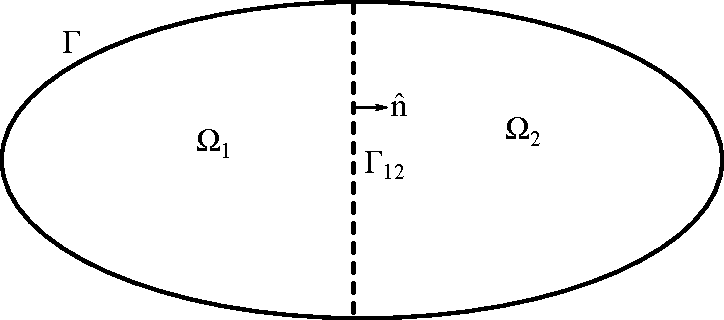
\includegraphics[width=8cm]{DDFETI}
\caption{FETI-DP based domain decomposition sketch for two subdomains.}
\label{fig:DDFETI}
\end{figure}

Let us consider the problem depicted by Fig. \ref{fig:DDFETI}. We seek to solve the following distinct boundary value problems defined as

\begin{equation}
\label{eq:FETID1}
\left\lbrace
\begin{aligned}
\nabla \times \frac{1}{\mu_r} \nabla \times {\mathbf{E}^1} + j k_0 \zeta_0 \sigma {\mathbf{E}^1} - k_0^2 \epsilon_r {\mathbf{E}^1} = 0,& \quad \mathrm{in} \ \Omega_1,\\[10pt]
\hat{\mathbf{n}} \times ( {\mathbf{E}^1} \times \hat{\mathbf{n}}) = 0, &\quad \mathrm{on} \ \mathrm{\Gamma}_E \cap d\Omega_1, \\[5pt]
\hat{\mathbf{n}} \times ( {\mathbf{H}^1} \times \hat{\mathbf{n}}) = 0, &\quad  \mathrm{on} \ \mathrm{\Gamma}_{H} \cap d\Omega_1, \\[5pt]
\hat{\mathbf{n}} \times \mathbf{H}^1 = \frac{1}{Z_s} \hat{\mathbf{n}} \times \hat{\mathbf{n}} \times \mathbf{E}^1 + \hat{\mathbf{n}} \times \mathbf{H}^{inc} - \frac{1}{Z_s} \hat{\mathbf{n}} \times \hat{\mathbf{n}} \times \mathbf{E}^{inc}, &\quad \mathrm{on} \ \Gamma_{R} \cap d\Omega_1, \\[5pt]
\hat{\mathbf{n}} \times \mathbf{H}_t^{1,k} = \frac{1}{Z_k} \hat{\mathbf{n}} \times \hat{\mathbf{n}} \times \mathbf{E}_t^{1,k} - \frac{2}{Z_k} \hat{\mathbf{n}} \times \hat{\mathbf{n}} \times \mathbf{E}_t^{k \ inc}, &\quad \mathrm{on} \ \Gamma_{WG}^k \cap d\Omega_1,\\[5pt]
\hat{\mathbf{n}} \times \frac{1}{\mu_r} \nabla \times \mathbf{E}^1 - jk_0 \ \hat{\mathbf{n}} \times \mathbf{E}^1 \times \hat{\mathbf{n}} = \qquad \qquad &\\ - \hat{\mathbf{n}} \times \frac{1}{\mu_r} \nabla \times \mathbf{E}^2 - jk_0 \ \hat{\mathbf{n}} \times \mathbf{E}^2 \times \hat{\mathbf{n}},  &\quad \mathrm{on} \ \Gamma_{12} \cap d\Omega_1, \\[5pt]
\end{aligned}
\right.
\end{equation}
%
\noindent and 
%
\begin{equation}
\label{eq:FETID2}
\left\lbrace
\begin{aligned}
\nabla \times \frac{1}{\mu_r} \nabla \times {\mathbf{E}^2} + j k_0 \zeta_0 \sigma {\mathbf{E}^2} - k_0^2 \epsilon_r {\mathbf{E}^2} = 0,& \quad \mathrm{in} \ \Omega_2,\\[10pt]
\hat{\mathbf{n}} \times ( {\mathbf{E}^2} \times \hat{\mathbf{n}}) = 0,& \quad \mathrm{on} \ \mathrm{\Gamma}_E \cap d\Omega_2, \\[5pt]
\hat{\mathbf{n}} \times ( {\mathbf{H}^2} \times \hat{\mathbf{n}}) = 0,& \quad  \mathrm{on} \ \mathrm{\Gamma}_{H} \cap d\Omega_2, \\[5pt]
\hat{\mathbf{n}} \times \mathbf{H}^2 = \frac{1}{Z_s} \hat{\mathbf{n}} \times \hat{\mathbf{n}} \times \mathbf{E}^2 + \hat{\mathbf{n}} \times \mathbf{H}^{inc} - \frac{1}{Z_s} \hat{\mathbf{n}} \times \hat{\mathbf{n}} \times \mathbf{E}^{inc},& \quad \mathrm{on} \ \Gamma_{R} \cap d\Omega_2, \\[5pt]
\hat{\mathbf{n}} \times \mathbf{H}_t^{2,k} = \frac{1}{Z_k} \hat{\mathbf{n}} \times \hat{\mathbf{n}} \times \mathbf{E}_t^{2,k} - \frac{2}{Z_k} \hat{\mathbf{n}} \times \hat{\mathbf{n}} \times \mathbf{E}_t^{k \ inc},& \quad \mathrm{on} \ \Gamma_{WG}^k \cap d\Omega_2,\\[5pt]
\hspace{-1cm}\hat{\mathbf{n}} \times \frac{1}{\mu_r} \nabla \times \mathbf{E}^2 - jk_0 \ \hat{\mathbf{n}} \times \mathbf{E}^2 \times \hat{\mathbf{n}} = \qquad \qquad &\\ - \hat{\mathbf{n}} \times \frac{1}{\mu_r} \nabla \times \mathbf{E}^1 - jk_0 \ \hat{\mathbf{n}} \times \mathbf{E}^1 \times \hat{\mathbf{n}},& \quad \mathrm{on} \ \Gamma_{21} \cap d\Omega_2,
\end{aligned}
\right.
\end{equation}

\noindent where the superscript on the fields $i \in \lbrace 1,2 \rbrace$ correspond to the fields spanned in the $i^\mathrm{th}$ domain ($\Omega_i$) and $d\Omega_i$ is the whole boundary of $\Omega_i$. $\hat{\mathbf{n}}$ is chosen, as done previously, to be outwardly directed from the subproblem domain. Notice that, in the conditions on $\Gamma_R$, if the incident fields vanish, the condition resorts to the classical absorbing boundary condition \eqref{eq:ABC}. The last boundary condition in each problem corresponds the \textit{Robin-Robin transmission condition}, pioneered by Despr\'es in 1991 \cite{Despres1991,Despres1992}, proving the convergence in an iterative solution of the coarse problem. In fact, direct imposition of the continuity of the tangential components of electric and magnetic fields may lead to internal resonances within subdomain problems, and the overall system matrix (see later) could be ill conditioned and hence may suffer from slow convergence or even fail to converge.

Let $\mathcal{W}_E^1$ and $\mathcal{W}_E^2$ be the $\mathcal{H}(\mathrm{curl})$-conforming space spanning the electric field solution such that
\begin{gather*}
\mathcal{W}_E^1 := \{ \mathbf{w} \in \mathcal{H}(\mathrm{curl},\Omega_1, \Gamma_E) \ | \ \hat{\mathbf{n}} \times \mathbf{w} = 0 \ \mathrm{on} \ \Gamma_E \},\\
\mathcal{W}_E^2 := \{ \mathbf{w} \in \mathcal{H}(\mathrm{curl},\Omega_2, \Gamma_E) \ | \ \hat{\mathbf{n}} \times \mathbf{w} = 0 \ \mathrm{on} \ \Gamma_E \},
\end{gather*}
%
\noindent and $\mathcal{H}(\mathrm{curl},\Omega, \Gamma_E) \equiv \mathcal{H}(\mathrm{curl},\Omega_1, \Gamma_E) \times \mathcal{H}(\mathrm{curl},\Omega_2, \Gamma_E)$. The Galerkin framework leads to the following weak form
%
\begin{multline}
\label{eq:FETIform1}
\int_{\Omega_1} \nabla \times \mathbf{w}_i^* \cdot \frac{1}{\mu_r} \nabla \times \mathbf{E}^1 \ d\Omega +
 j k_0 \zeta_0 \int_{\Omega_1} \mathbf{w}_i^* \cdot \sigma \mathbf{E}^1 \ d\Omega \ - \\
 k_0^2 \int_{\Omega_1} \mathbf{w}_i^* \cdot \epsilon_r \mathbf{E}^1 \ d\Omega \ + \int_{d\Omega_1} \mathbf{w}_i^* \cdot \hat{\mathbf{n}} \times \frac{1}{\mu_r} \nabla \times {\mathbf{E}^1}  \ d\Gamma = 0, 
\qquad \forall \mathbf{w}_i \in \mathcal{W}_E^1,
\end{multline}
\noindent and for the second subdomain
\begin{multline}
\label{eq:FETIform2}
\int_{\Omega_2} \nabla \times \mathbf{w}_i^* \cdot \frac{1}{\mu_r} \nabla \times \mathbf{E}^2 \ d\Omega +
 j k_0 \zeta_0 \int_{\Omega_2} \mathbf{w}_i^* \cdot \sigma \mathbf{E}^2 \ d\Omega \ - \\
 k_0^2 \int_{\Omega_2} \mathbf{w}_i^* \cdot \epsilon_r \mathbf{E}^2 \ d\Omega \ + \int_{d\Omega_2} \mathbf{w}_i^* \cdot \hat{\mathbf{n}} \times \frac{1}{\mu_r} \nabla \times {\mathbf{E}^2}  \ d\Gamma = 0, 
\qquad \forall \mathbf{w}_i \in \mathcal{W}_E^2.
\end{multline}
%
\noindent The integrals on $d\Omega_1$ and $d\Omega_2$ take into account all the \quotes{classical} boundary conditions seen in chapter \ref{chap:FE}, in particular $\Gamma_R$ and $\Gamma_{WG}$ which allow to excite the finite element domain. On $\Gamma_{12}$ and $\Gamma_{21}$, we introduce a coupling term in order to allow the boundary values to vary, enforcing in such a way the continuity of the function between adjacent subdomains. For instance,
\begin{gather}
\int_{\Gamma_{12}} \mathbf{w}_i^* \cdot \hat{\mathbf{n}} \times \frac{1}{\mu_r} \nabla \times {\mathbf{E}^1}  \ d\Gamma,\label{eq:j1}\\
\int_{\Gamma_{21}} \mathbf{w}_i^* \cdot \hat{\mathbf{n}} \times \frac{1}{\mu_r} \nabla \times {\mathbf{E}^2}  \ d\Gamma,\label{eq:j2}
\end{gather}
\noindent are non-null quantities on, respectively, $\Gamma_{12}$ and $\Gamma_{21}$.
%
\noindent We consequently introduce, to simplify our treatment, fictitious variables $\mathbf{j}^1$ and $\mathbf{j}^2$, defined as
\begin{eqnarray}
\mathbf{j}^1 & = & \frac{1}{k_0} \hat{\mathbf{n}} \times \frac{1}{\mu_r} \nabla \times {\mathbf{E}^1},\\
\mathbf{j}^2 & = & \frac{1}{k_0} \hat{\mathbf{n}} \times \frac{1}{\mu_r} \nabla \times {\mathbf{E}^2},
\end{eqnarray}
\noindent which correspond to the dual unknowns used as Lagrange multipliers in the FETI-DP algorithm. Let $\mathcal{V}_J^i$ be the spanning space for boundary constraints $\mathbf{v}$ on $\Gamma_{ij}, i, j \in \lbrace1,2 \ | \ i \neq j\rbrace$, such that
$$\mathcal{V}_J^i := \{ \mathbf{v} \in \mathcal{H}(\mathrm{curl},\Gamma_{ij}) \},$$
\noindent and 
\begin{eqnarray}
\label{eq:auxfieldExp}
\mathbf{j}^1 &:= & \sum_{l=1}^{N^1} \lambda_j \mathbf{v}_j^1, \qquad \mathbf{v}_j^1 \in \mathcal{V}_J^1, \nonumber \\
\mathbf{j}^2 &:= & \sum_{l=1}^{N^2} \lambda_j \mathbf{v}_j^2, \qquad \mathbf{v}_j^2 \in \mathcal{V}_J^2.\nonumber
\end{eqnarray}
\noindent Finally, the coupling terms in the Galerkin projections on each subdomain, respectively \eqref{eq:j1} and \eqref{eq:j2}, can be written as
\begin{eqnarray}
\int_{\Gamma_{12}} \mathbf{w}_i^* \cdot k_0 \ \mathbf{j}^1 \ d\Gamma &= &\sum_{l=1}^{N^1} \lambda_j k_0 \int_{\Gamma_{12}} \mathbf{w}_i^* \cdot \mathbf{v}_j \ d\Gamma, \quad \forall \mathbf{w}_i \in \mathcal{W}_E^1, \mathbf{v}_j \in \mathcal{V}_J^1, \label{eq:j1form}\\
\int_{\Gamma_{21}} \mathbf{w}_i^* \cdot k_0 \ \mathbf{j}^2 \ d\Gamma &= &\sum_{l=1}^{N^2} \lambda_j k_0 \int_{\Gamma_{21}} \mathbf{w}_i^* \cdot \mathbf{v}_j \ d\Gamma, \quad \forall \mathbf{w}_i \in \mathcal{W}_E^2, \mathbf{v}_j \in \mathcal{V}_J^2.\label{eq:j2form}
\end{eqnarray}
%
\noindent The Robin-Robin transmission conditions can also be written as
\begin{equation}
\label{eq:RRTC}
\left\lbrace
\begin{aligned}
j k_0 \ \mathbf{j}^1 + k_0 \ \hat{\mathbf{n}} \times \mathbf{E}^1 \times \hat{\mathbf{n}} &=  - jk_0 \ \mathbf{j}^2 + k_0 \ \hat{\mathbf{n}} \times \mathbf{E}^2 \times \hat{\mathbf{n}},& \quad \mathrm{on} \ \Gamma_{12} \cap d\Omega_1,\\
j k_0 \ \mathbf{j}^2 + k_0 \ \hat{\mathbf{n}} \times \mathbf{E}^2 \times \hat{\mathbf{n}} &=  - jk_0 \ \mathbf{j}^1 + k_0 \ \hat{\mathbf{n}} \times \mathbf{E}^1 \times \hat{\mathbf{n}},& \quad \mathrm{on} \ \Gamma_{21} \cap d\Omega_2,
\end{aligned}
\right.
\end{equation}
\noindent where we have multiplied both sides of the equations by $j$ to achieve a better conditioning of the resulting matrices.

\noindent To introduce coupling between subdomains, further Galerkin projections are performed by testing the transmission conditions with $\mathbf{v}_i \in \mathcal{V}_J^1$ for the first subproblem and $\mathbf{v}_i \in \mathcal{V}_J^2$ for the second one. As a result,
\begin{multline}
j k_0 \ \int_{\Gamma_{12}} \mathbf{v}_i^* \cdot \mathbf{j}^1 \ d\Gamma + k_0 \ \int_{\Gamma_{12}} \mathbf{v}_i^* \cdot \hat{\mathbf{n}} \times \mathbf{E}^1 \times \hat{\mathbf{n}} \ d\Gamma = \\
- jk_0 \ \int_{\Gamma_{12}} \mathbf{v}_i^* \cdot \mathbf{j}^2 \ d\Gamma + k_0 \
\int_{\Gamma_{12}} \mathbf{v}_i^* \cdot \hat{\mathbf{n}} \times \mathbf{E}^2 \times \hat{\mathbf{n}} \ d\Gamma, \qquad \forall \mathbf{v}_i \in \mathcal{V}_J^1,
\end{multline}
\noindent for the problem in $\Omega_1$ and
\begin{multline}
jk_0 \ \int_{\Gamma_{21}} \mathbf{v}_i^* \cdot \mathbf{j}^2 \ d\Gamma + k_0 \ \int_{\Gamma_{21}} \mathbf{v}_i^* \cdot \hat{\mathbf{n}} \times \mathbf{E}^2 \times \hat{\mathbf{n}} \ d\Gamma = \\
- jk_0 \ \int_{\Gamma_{21}} \mathbf{v}_i^* \cdot \mathbf{j}^1 \ d\Gamma + k_0 \
\int_{\Gamma_{21}} \mathbf{v}_i^* \cdot \hat{\mathbf{n}} \times \mathbf{E}^1 \times \hat{\mathbf{n}} \ d\Gamma, \qquad \forall \mathbf{v}_i \in \mathcal{V}_J^2,
\end{multline}
\noindent on $\Omega_2$.


\begin{figure}[ht!]
\centering
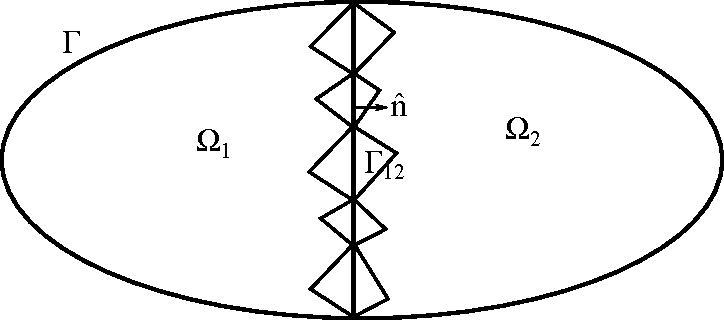
\includegraphics[width=8cm]{DDConforming}
\caption{Conforming domain decomposition sketch for two subdomains.}
\label{fig:DDConforming}
\end{figure}

Throughout this dissertation, the mesh is assumed to be conforming between adjacent domains, that is, all the elements at the boundaries are connected at their nodes as depicted in Fig. \ref{fig:DDConforming}. The choice of $\mathbf{v} = \hat{\mathbf{n}} \times \mathbf{w}$ has resulted, in terms of simplicity and convergence speed, the best choice. $\mathbf{v} = \hat{\mathbf{n}} \times \mathbf{w} \times \hat{\mathbf{n}}$ led to slower convergence in the iterative FETI-DP solution. The previous weak forms lead to the following systems
\begin{equation}
\label{eq:DDFETI1}
\begin{bmatrix}
A_{11} & A_{\Gamma_1 1} & \\
A_{\Gamma_1 1}^T & A_{\Gamma_1 \Gamma_1} & D_{11}\\
 & D_{11}^T  & T_{11}
\end{bmatrix}
\begin{bmatrix}
x_{1}\\
x_{\Gamma_1}\\
\lambda_{1}
\end{bmatrix}
=
\begin{bmatrix}
B_{1}\\
B_{\Gamma_1}\\
\phantom{x}
\end{bmatrix}
+
\begin{bmatrix}
\phantom{-}\phantom{A} & \phantom{-}\phantom{A} & \phantom{A}\\
\phantom{A} & \phantom{A} & \phantom{A}\\
\phantom{A} & D_{12}  & -T_{12}
\end{bmatrix}
\begin{bmatrix}
\phantom{A}\\
x_{\Gamma_2}\\
\lambda_{2}
\end{bmatrix},
\end{equation}
\noindent for the first subproblem and 
\begin{equation}
\label{eq:DDFETI2}
\begin{bmatrix}
A_{22} & A_{\Gamma_2 2} & \\
A_{\Gamma_2 2}^T & A_{\Gamma_2 \Gamma_2} & D_{22}\\
 & D_{22}^T  & T_{22}
\end{bmatrix}
\begin{bmatrix}
x_{2}\\
x_{\Gamma_2}\\
\lambda_{1}
\end{bmatrix}
=
\begin{bmatrix}
B_{2}\\
B_{\Gamma_2}\\
\phantom{x}
\end{bmatrix}
+
\begin{bmatrix}
\phantom{-}\phantom{A} & \phantom{-}\phantom{A} & \phantom{A}\\
\phantom{A} & \phantom{A} & \phantom{A}\\
\phantom{A} & D_{21}  & -T_{21}
\end{bmatrix}
\begin{bmatrix}
\phantom{x}\\
x_{\Gamma_1}\\
\lambda_{1}
\end{bmatrix},
\end{equation}
\noindent for the second one. The block matrices $\mat{A_{\Omega\Omega}}$, $\mat{A_{\Gamma_{\Omega}\Omega}}$ are $\mat{A_{\Gamma_{\Omega}\Gamma_{\Omega}}}$ those computed as in section \ref{sec:SchurDD}. The last block $\mat{D_{\Gamma\Gamma}}$ is the one that is retrieved by the coupling term integrals of \eqref{eq:j1} and \eqref{eq:j2}. The last row of block-matrices is retrieved by the testing of the transmission conditions \eqref{eq:RRTC} with the dual shape functions $\mathbf{v}$.
Explicitly, we have
\begin{gather*}
D_{mm} = k_0 \ \int_{\Gamma_{mn}} {\mathbf{v}_i^{m}}^* \cdot \hat{\mathbf{n}} \times\mathbf{w}_j^m \times \hat{\mathbf{n}} \ d\Gamma, \\
T_{mm} = jk_0 \ \int_{\Gamma_{mn}} {\mathbf{v}_i^{m}}^* \cdot \mathbf{v}_j^m \ d\Gamma,\\
D_{mn} = k_0 \ \int_{\Gamma_{mn}} {\mathbf{v}_i^{m}}^* \cdot \hat{\mathbf{n}} \times\mathbf{w}_j^n \times \hat{\mathbf{n}} \ d\Gamma, \\
T_{mn} = jk_0 \ \int_{\Gamma_{mn}} {\mathbf{v}_i^{m}}^* \cdot \mathbf{v}_j^n \ d\Gamma.
\end{gather*}
%
The systems of \eqref{eq:DDFETI1} and \eqref{eq:DDFETI2} can be solved directly in an alternating fashion within an iterative procedure. Starting from null solution vectors for each subdomain, $\mat{x}_1 = \mat{x_1 \ x_{\Gamma_1} \ \lambda_1}^T$ and $\mat{x}_2 = \mat{x_2 \ x_{\Gamma_2} \ \lambda_2}^T$, the procedure is expressed by the algorithm \ref{alg:FETIWISE}.
\begin{algorithm}[ht!]
\begin{algorithmic}
\caption{Domain-wise FETI-DP solution procedure.}
\label{alg:FETIWISE}
\State $\mat{x}_1^0 \gets 0$
\State $\mat{x}_2^0 \gets 0$
\State $k \gets 1$
\State $\mathit{err} \gets 1$
\While {$\mathit{err} \geq \mathit{maxerr}$}
    \State $\mat{x}_1^k \gets$ Solve \eqref{eq:DDFETI1}
    \State $\mat{x}_2^k \gets$ Solve \eqref{eq:DDFETI2}
    \State $\mathit{err} \gets \max \left(\frac{\Vert \mat{x}_1^k - \mat{x}_1^{k-1} \Vert}{\Vert \mat{x}_1^k\Vert}, \frac{\Vert \mat{x}_2^k - \mat{x}_2^{k-1} \Vert}{\Vert \mat{x}_2^k\Vert}\right)$ 
    \State $k \gets k+1$
\EndWhile
\end{algorithmic}
\end{algorithm}

One can also restrict the iterative procedure to the dual-primal unknowns. First a restriction matrix (boolean matrix) $\mat{R}_1$ is built as
$$ \mat{R}_1 = \begin{bmatrix}
\phantom{I_{P_1}} & I_{P_1} & \\
& & I_{D_1}
\end{bmatrix},$$
\noindent where $\mat{I_{P_1}}$ and $\mat{I_{D_1}}$ are unitary matrices of the size, respectively, of the number of primal and dual unknowns. Notice that the sizes might be different if $\Gamma_E$ crosses the boundary $\Gamma_{12}$. Than, the solution process is changed upon apply restriction to the subdomains solution vectors
%
\begin{multline}
\label{eq:DDFETI1res}
\begin{bmatrix}
x_{\Gamma_1}\\
\lambda_{1}
\end{bmatrix} =
\mat{R}_1
\begin{bmatrix}
x_{1}\\
x_{\Gamma_1}\\
\lambda_{1}
\end{bmatrix}
=\\
\mat{R}_1
\begin{bmatrix}
A_{11} & A_{\Gamma_1 1} & \\
A_{\Gamma_1 1}^T & A_{\Gamma_1 \Gamma_1} & D_{11}\\
 & D_{11}^T  & T_{11}
\end{bmatrix}^{-1}
\left(
\begin{bmatrix}
B_{1}\\
B_{\Gamma_1}\\
\phantom{x}
\end{bmatrix}
+
\begin{bmatrix}
\phantom{-}\phantom{A} & \phantom{-}\phantom{A} & \phantom{A}\\
\phantom{A} & \phantom{A} & \phantom{A}\\
\phantom{A} & D_{12}  & -T_{12}
\end{bmatrix}
\begin{bmatrix}
\phantom{x}\\
x_{\Gamma_2}\\
\lambda_{2}
\end{bmatrix}
\right) = \\
\underbrace{
\mat{R}_1
\begin{bmatrix}
A_{11} & A_{\Gamma_1 1} & \\
A_{\Gamma_1 1}^T & A_{\Gamma_1 \Gamma_1} & D_{11}\\
 & D_{11}^T  & T_{11}
\end{bmatrix}^{-1}
}_{(1)}
\left(
\begin{bmatrix}
B_{1}\\
B_{\Gamma_1}\\
\phantom{x}
\end{bmatrix}
+
\begin{bmatrix}
\phantom{A} & \phantom{A}\\
\phantom{A} & \phantom{A}\\
D_{12}  & -T_{12}
\end{bmatrix}
\begin{bmatrix}
x_{\Gamma_2}\\
\lambda_{2}
\end{bmatrix}
\right).
\end{multline}
\noindent Analogous matrices are computed for the second subproblem upon performing the changes in the subscripts $2 \rightarrow 1$ and $1 \rightarrow 2$. Notice that restriction matrices may result different for the second subproblem. The matrix factor $(1)$ lead to a small rectangular matrix (the row size is as the number of primal and dual unknowns on the boundaries) but dense due to matrix inversion. Once the procedure converged, the whole solution can be recovered by the solution of \eqref{eq:DDFETI1} and \eqref{eq:DDFETI2} where the dual and primal unknowns of the coarse problem provide the correct boundary conditions for continuity.

Several works\cite{Vouvakis2004,lee2005non,Vouvakis2006, li2006vector} have exploited the repetition of subdomains problems such as in finite periodic analyzes to considerably reduce the amount of matrices factors to compute. However, as we seek for the solution of arbitrarily shaped problems, the construction of many dense matrices may not be profitable. Hence, the path of constructing domain decomposition based preconditioners for Krylov subspace iterative solvers have been taken, as will be shown in the next sections. For this purpose, we formulate the global FETI-DP system to be solved with an iterative method as, collecting both systems \eqref{eq:DDFETI1} and \eqref{eq:DDFETI2} in a single global system,

\begin{equation}
\label{eq:FETIDPFull}
\begin{bmatrix}
A_{11} & A_{\Gamma_1 1} & & & & \\
A_{\Gamma_1 1}^T & A_{\Gamma_1 \Gamma_1} & D_{11} & & &\\
 & D_{11}^T  & T_{11} & \phantom{A} & -D_{12}  & T_{12}\\
& & & A_{22} & A_{\Gamma_2 2} &  \\
& & & A_{\Gamma_2 2}^T & A_{\Gamma_2 \Gamma_2} & D_{22}\\
\phantom{A} & -D_{21}  & T_{21} & & D_{22}^T  & T_{22}
\end{bmatrix}
\begin{bmatrix}
x_{1}\\
x_{\Gamma_1}\\
\lambda_{1}\\
x_{2}\\
x_{\Gamma_2}\\
\lambda_{2}
\end{bmatrix}
=
\begin{bmatrix}
\phantom{x}\\
B_{\Gamma_1}\\
\phantom{x}\\
\phantom{x}\\
B_{\Gamma_2}\\
\phantom{x}\\
\end{bmatrix}.
\end{equation}

\section[DD preconditioners for Krylov solvers]{Domain decomposition based preconditioners for \\Krylov subspace iterative solvers}

In this section, we present the Krylov subspace iterative solvers which exploit the optimality properties of projections (on Krylov spaces) during the iterative search process of the solution, with a deep control on the residual error (with error bounds) \cite{saad2000iterative}. In particular, we have employed the \textit{restarted-Generalized Minimum Residual} (GMRES($r$)) which finds the steepest descent upon applying projections in the residual norm between successive refinements of the solution. Its restarted approach is such that the basis vectors spanning the solution is restricted to a given number $r$, allowing to save memory requirements. Of course, the retarded version leads to different results respectively to the non-restarted version, as the whole projection bases are reset after $r$ iterations, and the next iteration cycle may start with a higher residual error.


\subsection{Restarted-Generalized Minimum Residual}

A general projection method for solving a linear system 
$$ \mat{A} \vect{x} = \vect{b}, $$ 
\noindent extracts an approximate solution $\vect{x}_m$ from an affine subspace $\vect{x}_0 + \mathcal{K}_m$ of dimension $m$ by imposing the Petrov-Galerkin condition
$$ \vect{b} - \mat{A}\vect{x}_m \perp \mathcal{L}_m$$
\noindent where $\mat{\mathcal{L}}_m$ is another subspace of dimension $m$. $\mat{x}_0$ is an initial guess to the solution.
A Krylov subspace method is such that
$$\mathcal{K}_m(\mat{A},\vect{r}_0) = \mathrm{span}\{\vect{r}_0, \mat{A}\vect{r}_0, \mat{A}^2\vect{r}_0,\ldots,\mat{A}^{m-1}\vect{r}_0\} $$
\noindent where $\vect{r}_0 = \vect{b}-\mat{A}\vect{x}_0$ is the residual. The vectors spanning $\mathcal{K}_m(\mat{A},\vect{r}_0)$ might be almost linearly dependent. Thus, an appropriate orthonormalization is employed to build a Krylov subspace basis $\mat{V}_m = \mathrm{span}\{\vect{v}_1,\ldots,\vect{v}_m \}$, the \textit{Arnoldi-Modified Gram-Schmidt} algorithm \ref{alg:Arnoldi}.
\begin{algorithm}[ht!]
\begin{algorithmic}
\caption{Arnoldi-Modified Gram-Schmidt.}
\label{alg:Arnoldi}
\State Choose a vector $\vect{v}_1$ such that $\Vert \vect{v}_1 \Vert_2 = 1$
\For {j = 1, \ldots, m}
    \State $\vect{w}_j \gets \mat{A} \vect{v}_j$
    \For {i = 1, \ldots, j}
    	\State $h_{i,j} \gets <\vect{w}_j,\vect{v}_i>$
		\State $\vect{w}_j \gets \vect{w}_j - h_{i,j} \vect{v}_i$
    \EndFor
    \State $h_{j+1,j} \gets \Vert \vect{w}_j \Vert_2$
    \If {$h_{j+1,j} = 0$} \State Break \EndIf
    \State $\vect{v}_{j+1} \gets \nicefrac{\vect{w}_j}{h_{j+1,j}} $
\EndFor
\end{algorithmic}
\end{algorithm}
%
\noindent The Arnoldi process produces and $\mathbb{R}^{m+1 \times m}$ upper Hessenberg matrix $\mat{H}_m$, coefficients for the expansion of $\mat{A}$ such that
\begin{eqnarray}
\label{eq:Hess}
\mat{A} \mat{V}_m &= &\mat{V}_{m+1} \mat{H}_m
\end{eqnarray}
\noindent Any vector $\vect{x} \in \vect{x}_0 + \mathcal{K}_m$ can be now written as
$$\vect{x} = \vect{x}_0 + \mat{V}_m \vect{y}$$
\noindent where $\vect{y}$ is a vector of dimension $m$. Defining 
$$J(\vect{y}) = \Vert \vect{b} - \mat{A} \vect{x} \Vert_2 = \Vert \vect{b} - \mat{A} (\vect{x}_0 + \mat{V}_m \vect{y})\Vert_2,$$
\noindent the relation \eqref{eq:Hess} results in
\begin{eqnarray*}
\vect{b} - \mat{A} \mat{V}_m &= &\vect{b} - {A}(\vect{x}_0 + \mat{V}_m \vect{y}),\\
&= & \vect{r}_0 - \mat{A} \mat{V}_m \vect{y},\\
&= & \beta\vect{v}_1 - \mat{V}_{m+1} \mat{H}_m \vect{y},\\
&= & \mat{V}_{m+1} \left( \beta\vect{e}_1 - \mat{H}_m \vect{y}\right).
\end{eqnarray*}
\noindent with $\beta = \Vert \vect{r}_0 \Vert_2$ and $\vect{v}_1 = \vect{r}_0/\beta$ is the first vector of unitary norm chose in the first step of the algorithm \ref{alg:Arnoldi}, and $\mat{V}_m^T\vect{r}_0 = \mat{V}_m^T(\beta\vect{v}_1) = \beta\vect{e}_1$ with $\vect{e}_1 = \vect{1 \ 0 \ \ldots \ 0}^T$ is the first standard basis vector. Since the column-vectors spanning $\mat{V}_{m+1}$ are orthonormal, then
$$J(\vect{y}) = \Vert \vect{b} - \mat{A} (\vect{x}_0 + \mat{V}_m \vect{y})\Vert_2 = \Vert \beta\vect{e}_1 - \mat{H}_m \vect{y} \Vert_2.$$
\noindent The GMRES \cite{saad1986gmres} (not yet restarted) approximation is the unique vector of $\vect{x}_0 + \mathcal{K}_m$  which minimizes $J(\vect{y})$. The approximation is obtained as $$\vect{x}_m = \vect{x}_0 + \mat{V}_m \vect{y}_m,$$ where $$\vect{y}_m = \mathrm{argmin}_y \Vert \beta\vect{e}_1 - \mat{H}_m \vect{y} \Vert_2.$$
%
\begin{algorithm}[ht!]
\begin{algorithmic}
\caption{Restarted-Generalized Minimum Residual.}
\label{alg:rGMRES}
\While {$\beta = \Vert \vect{r}_0 \Vert_2 \geq \mathit{maxerr}$  with $\vect{r}_0 = \vect{b} - {A}(\vect{x}_0$, $\vect{v}_1 = \vect{r}_0/\beta$}
	\For {$m = 1,\ldots, r$}
	\State Generate the Arnoldi basis and $\mat{H}_m$
	\State Compute $\vect{y}_m$ which minimizes $\Vert \beta\vect{e}_1 - \mat{H}_m \vect{y} \Vert_2$ 
	\State Compute $\vect{x}_m = \vect{x}_0 + \mat{V}_m \vect{y}_m$
	\EndFor
	\State $\vect{x}_0 \gets \vect{x}_m$ \Comment{The new starting vector is $\vect{x}_m$}
\EndWhile
\end{algorithmic}
\end{algorithm}
%
%An important result on the convergence of symmetric positive definite matrices (as those analyzed ) is that
%$$\Vert \vect{r}_n \Vert_2 \leq \left(\frac{2 \mathsf{k}_2(\mat{A})-1}{2 \mathsf{k}_2(\mat{A})}\right)^{{n}/{2}} \Vert \vect{r}_0 \Vert_2$$
%\noindent where $\mathsf{k}_2(\mat{A})$ is the condition number of the system matrix.

A well known difficulty with the restarted GMRES algorithm is that it can stagnate
when the matrix is not positive-definite\footnote{Certain boundary conditions (especially for radiation and waveports continuity) and  materials properties may lead to non-positive-definite system matrices.}. The full GMRES algorithm is guaranteed to converge in at most $N$ steps ($N$ the system dimensions), but this would be impractical if there were many steps required for convergence, due to large memory requirements: $O(N^2)$, similar to sparse direct solvers, whereas the restarted has only $O(rN)$ memory requirements. 

A typical remedy is to use preconditioning techniques whose goal is to reduce the number of steps required to converge. Here follow two types of preconditioners: the block Jacobi and the block Gauss-Seidel. None of these involve the computation of a Schur complement matrix, as a direct assembly of this matrix and its inversion without proper approximation may lead, for very large problem, to memory bottlenecks.

\subsection{Block Jacobi preconditioner}\label{sec:JC}

Let us consider the linear system of equations that leads to the following matrix system 
\begin{equation}
\label{eq:SysBlocks}
\begin{bmatrix}
A_{11} & A_{12} & A_{13}\\
A_{21} & A_{22} & A_{23}\\
A_{31} & A_{32} & A_{33}
\end{bmatrix}
\begin{bmatrix}
x_{1}\\
x_{2}\\
x_{3}
\end{bmatrix}
=
\begin{bmatrix}
b_{1}\\
b_{2}\\
b_{3}
\end{bmatrix},
\end{equation}
\noindent where $\mat{A}$ is non necessarily symmetric and we have considered only a single right-hand side vector as the GMRES($r$) solves for one right-hand side at a time. The block Jacobi preconditioner is defined as
\begin{equation}
\label{eq:jc}
\mat{P}_{J}
=
\begin{bmatrix}
A_{11} &  & \\
 & A_{22} & \\
 & & A_{33}
\end{bmatrix},
\end{equation}
\noindent and the resulting preconditionned system is
\begin{multline}
\begin{bmatrix}
\mat{A_{11}}^{-1} &  & \\
 & \mat{A_{22}}^{-1} & \\
 & & \mat{A_{33}}^{-1}
\end{bmatrix}
\begin{bmatrix}
A_{11} & A_{12} & A_{13}\\
A_{21} & A_{22} & A_{23}\\
A_{31} & A_{32} & A_{33}
\end{bmatrix}
\begin{bmatrix}
x_{1}\\
x_{2}\\
x_{3}
\end{bmatrix}
=\\
\begin{bmatrix}
\mat{A_{11}}^{-1} &  & \\
 & \mat{A_{22}}^{-1} & \\
 & & \mat{A_{33}}^{-1}
\end{bmatrix}
\begin{bmatrix}
b_{1}\\
b_{2}\\
b_{3}
\end{bmatrix},
\end{multline}
\noindent where we have exploited the following relation on the inversion of block diagonal matrices
$$ 
\begin{bmatrix}
A_{11} &  & \\
 & A_{22} & \\
 & & A_{33}
\end{bmatrix}^{-1} = 
\begin{bmatrix}
\mat{A_{11}}^{-1} &  & \\
 & \mat{A_{22}}^{-1} & \\
 & & \mat{A_{33}}^{-1}
\end{bmatrix}.
$$
\noindent Preconditioning with $\mat{P}_{J}$ is integrated in the GMRES($r$) algorithm after the computation of the residual vector $\vect{r}_m = \vect{b} - \mat{A} (\vect{x}_0 + \mat{V}_m \vect{y}) = \vect{\vect{r_1}_m \ \vect{r_2}_m \ \vect{r_3}_m}^T$ upon performing
\begin{eqnarray*}
\vect{r_1}_m &\longleftarrow & \mat{A_{11}}^{-1}\vect{r_1}_m, \\
\vect{r_2}_m &\longleftarrow & \mat{A_{22}}^{-1}\vect{r_2}_m, \\
\vect{r_3}_m &\longleftarrow & \mat{A_{33}}^{-1}\vect{r_3}_m. 
\end{eqnarray*}

\subsection{Block Gauss-Seidel preconditioner} \label{sec:GS}

Let us consider again the matrix system \eqref{eq:SysBlocks}, the lower block Gauss-Seidel preconditioner is defined as
\begin{equation}
\label{eq:gs}
\mat{P}_{GS}
=
\begin{bmatrix}
A_{11} &  & \\
A_{21} & A_{22} & \\
A_{31} & A_{32} & A_{33}
\end{bmatrix}.
\end{equation}
\noindent The inversion of the whole $\mat{P}_{GS}$ results, in the case of symmetric Schur complement based domain decomposition, to the solution of the problem, hence at the cost of a direct solver. In any case, the computational requirements may be prohibitive for large problems. However, it can be shown that the inverse of $\mat{P}_{GS}$
\begin{gather}
\begin{bmatrix}
A_{11} &  & \\
A_{21} & A_{22} & \\
A_{31} & A_{32} & A_{33}
\end{bmatrix}^{-1} = 
\begin{bmatrix}
\mat{A_{11}}^{-1} &  & \\
\tilde{\mat{A_{21}}} & \mat{A_{22}}^{-1} & \\
\tilde{\mat{A_{31}}} & \tilde{\mat{A_{32}}} & \mat{A_{33}}^{-1}
\end{bmatrix},
\end{gather}
\noindent where
\begin{eqnarray*}
\tilde{\mat{A_{21}}} &= &-\mat{A_{22}}^{-1}\mat{A_{21}}\mat{A_{11}}^{-1},\\
\tilde{\mat{A_{32}}} &= &-\mat{A_{33}}^{-1} \mat{A_{32}} \mat{A_{22}}^{-1},\\
\tilde{\mat{A_{31}}} &= &\mat{A_{33}}^{-1}\mat{A_{32}}\mat{A_{22}}^{-1}\mat{A_{21}}\mat{A_{11}}^{-1}- \mat{A_{33}}^{-1}\mat{A_{31}}\mat{A_{11}}^{-1},
\end{eqnarray*}
\noindent can be computed sequentially on the residual vector, updating it progressively while computing the diagonal blocks inverse. Preconditioning with $\mat{P}_{GS}$ is integrated in the GMRES($r$) algorithm after the computation of the residual vector $\vect{r}_m = \vect{b} - \mat{A} (\vect{x}_0 + \mat{V}_m \vect{y}) = \vect{\vect{r_1}_m \ \vect{r_2}_m \ \vect{r_3}_m}^T$ upon performing sequentially
\begin{eqnarray*}
\vect{r_1}_m &\longleftarrow & \mat{A_{11}}^{-1}\vect{r_1}_m, \\
\vect{r_2}_m &\longleftarrow & \mat{A_{22}}^{-1}\left(\vect{r_2}_m - \mat{A_{21}} \vect{r_1}_m \right).\\
\vect{r_3}_m &\longleftarrow & \mat{A_{33}}^{-1}\left(\vect{r_3}_m - \mat{A_{31}} \vect{r_1}_m - \mat{A_{32}} \vect{r_2}_m\right).\\
\end{eqnarray*}


\section{Numerical tests}

In this section, we present several results on a simple test case, that of a WR-90 rectangular waveguide segment, where the mesh is partitioned in order to implement the domain decomposition formulations. First, a simple two-domains test will be performed to assess the methods without iterative solvers. Then, the performances of the preconditioners will be analyzed, also varying the number of subdomains. %Finally, the analysis of a FSS-radome enclosed patch antennas array will be tackled.

\subsection{WR-90 rectangular waveguide}

The model analyzed consists of a 240~mm long $\hat{\mathbf{x}}$-directed WR-90 waveguide segment. The metallic walls are considered perfect electric conductors  while the two waveports are located at the extremities in the $\hat{\mathbf{x}}$ direction. The mesh consists of 20~602 tetrahedra and has been partitioned, using Metis \cite{karypis1995metis}, into two parts separated by an arbitrarily shaped surface composed by faces shared by tetrahedra located in the middle of the segment. Actually, Metis divides a mesh such that the parts result to have approximately the same number of tetrahedra (10~489 and 10~113).

\begin{figure}[h!]
\centering
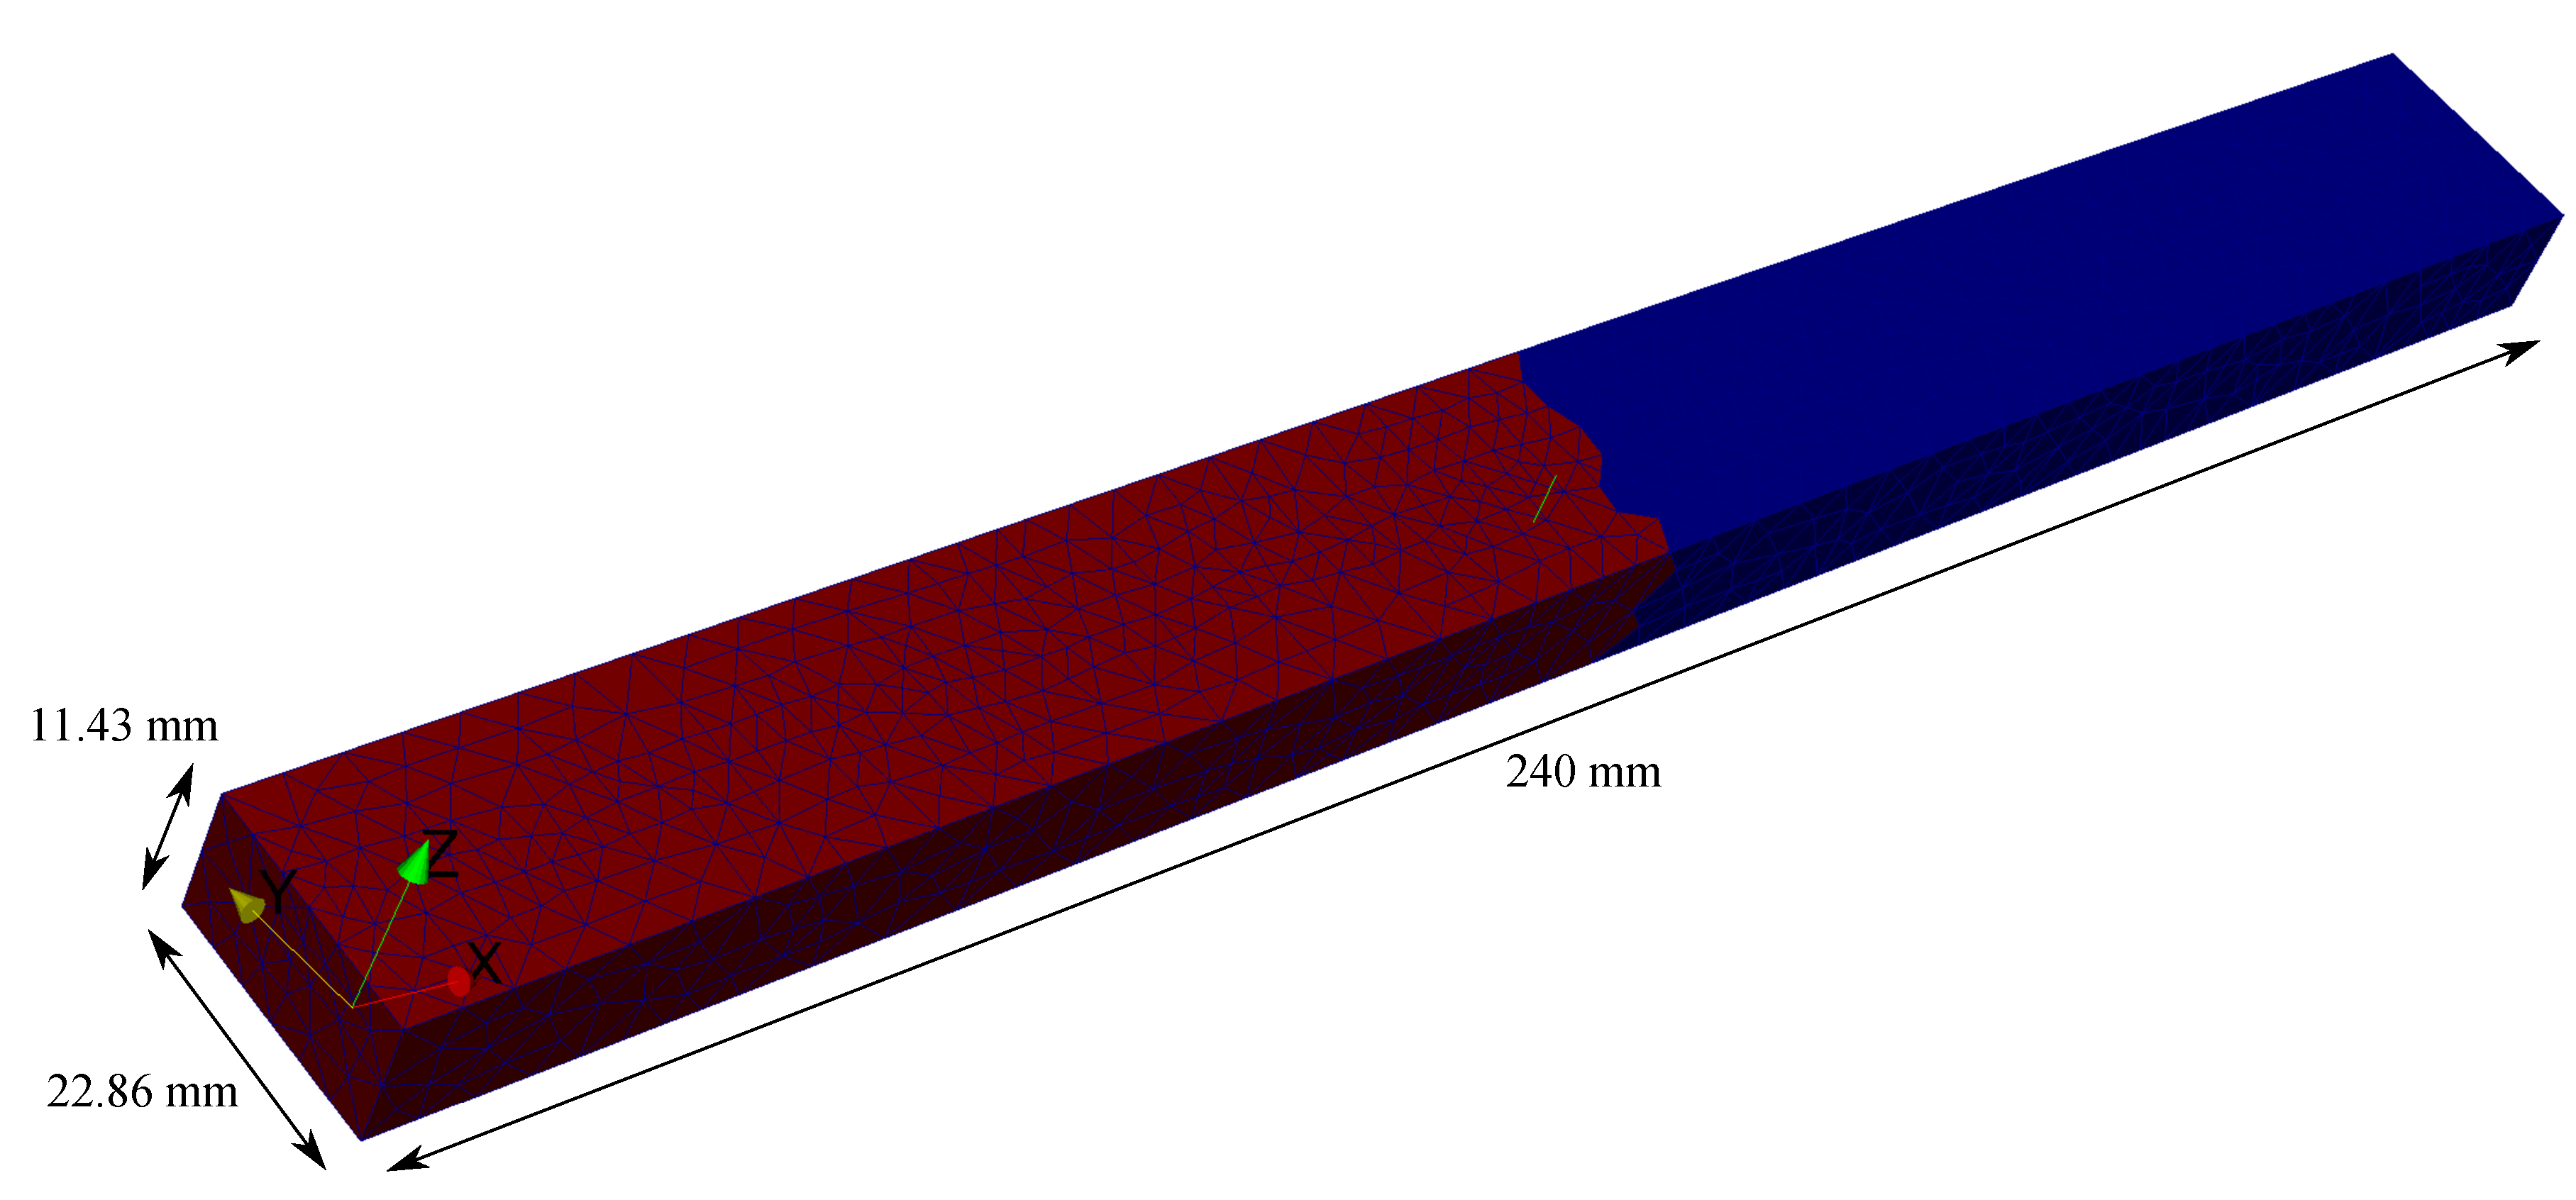
\includegraphics[width=13.4cm]{WR90Part}
\caption{$\hat{\mathbf{x}}$-directed WR-90 waveguide segment and conformal mesh partitioning.}
\label{fig:WR90Part}
\end{figure}

\subsection{Direct analysis}

The first conducted analysis is a direct solution of the whole problem upon imposing either dominant mode (DOM) or transfinite element method (TFE) on the waveports, and computing its spectral response over the mono-modal bandwidth. First order basis functions have been used to compute the scattering parameters ($\mathrm{TE}_{10}$) of Fig. \ref{fig:WRfreq}.

\begin{figure}[h!]
\centering
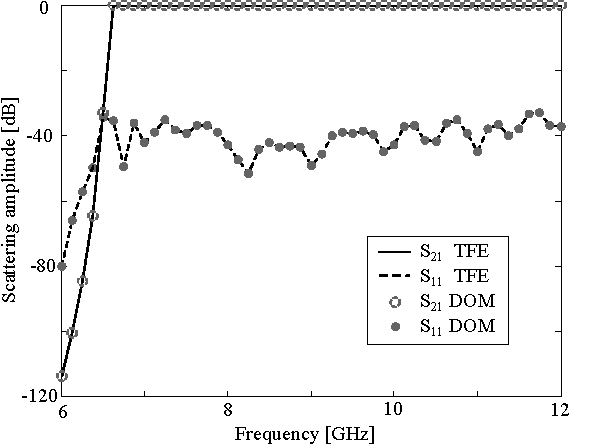
\includegraphics[width=10cm]{WRfreq}
\caption{Frequency response of the WR-90 waveguide segment.}
\label{fig:WRfreq}
\end{figure}

As expected, all the power is transmitted to the second port only when the frequency of excitation is higher than the cut-off frequency of 6.557 GHz for the $\mathrm{TE}_{10}$ mode in a WR-90. No significant differences are noticed between TFE and DOM for this frequency range. The peak memory required by the process was of about 50~MB and the times for assembly and solve of 0.7~s for each frequency point.

\subsection{Schur complement analysis}

Next, the Schur complement solution is performed. The assembled DD system matrix is shown in Fig. \ref{fig:DDSchurMat}. The assembly timings were of about 2.5~s. While the direct solution required only 0.45~s, the Schur approach required considerably more times and memory, as reported in table \ref{tab:SchurSol}. The assembly of the Schur complement matrix required approximately 10~s, due principally to the 155 column vectors of $\mat{A_{\Gamma 1}}^T$ which have to be multiplied by the dense matrix $\mat{A_{11}}^{-1}$. This step can be enhanced, exploiting the fact many of these column vectors are identically null. The computation of boundary unknowns is rather rapid and inexpensive for their small dimensions. The high density of the Schur complement matrix is shown in Fig. \ref{fig:DDSchurMatS}. Even if symmetries are exploited, the use of direct solvers ($O(N^3)$) would quickly lead to memory overload. The scattering parameters computed by this solution are reported in Fig. \ref{fig:WRfreqSchur} , as the maximum error recorded in this process has been of $\approx 10^{-12}$ in both TFE and DOM excitations.

\begin{table}[ht!]
\begin{center}
\begin{tabular}{|c|c|c|}
\hline 
Step & Time & Memory \\ 
\hline
\hline 
$\mat{A_{\Gamma 1}} \mat{A_{11}}^{-1} \mat{A_{\Gamma 1}}^T$ (8557) & 5.2~s & 10~MB\\ \hline 
$\mat{A_{\Gamma 2}} \mat{A_{22}}^{-1} \mat{A_{\Gamma 2}}^T$ (8082) & 4.8~s & 9.5~MB\\ \hline 
$\mat{x_\Gamma} = \mat{S}^{-1} \mat{G}$ (155) & 0.002~s & < 1~MB\\ \hline 
$\mat{x_1} = \mat{A_{11}}^{-1} (-\mat{A_{\Gamma 1}}^T \mat{x_\Gamma})$ & 0.15~s &  2~MB\\ \hline 
$\mat{x_2} = \mat{A_{22}}^{-1} (-\mat{A_{\Gamma 2}}^T \mat{x_\Gamma})$ & 0.14~s &  2~MB\\ \hline 
\end{tabular}
\end{center}
\caption{Direct Schur solution times and memory requirements.}
\label{tab:SchurSol}
\end{table}

\begin{figure}[ht!]
\centering
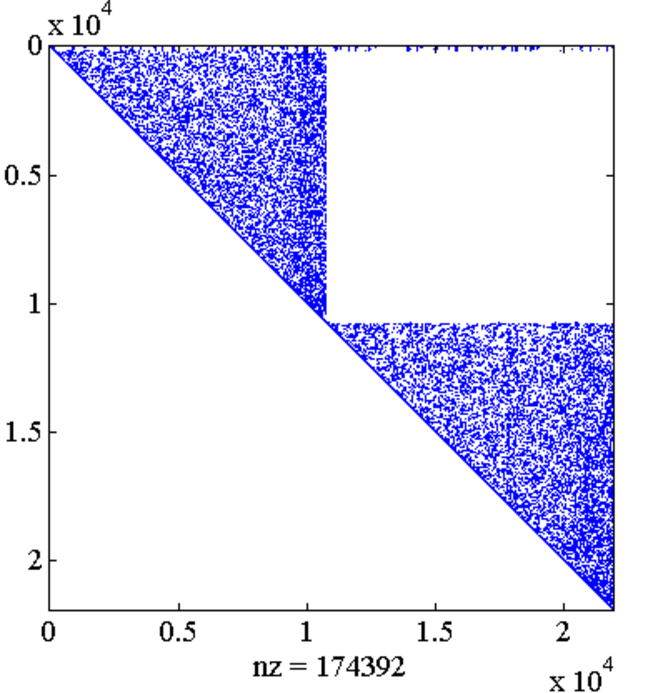
\includegraphics[width=10cm]{DDSchurMat}
\caption{Upper triangular part of the Schur complement based domain decomposition system matrix.}
\label{fig:DDSchurMat}
\end{figure}

\begin{figure}[ht!]
\centering
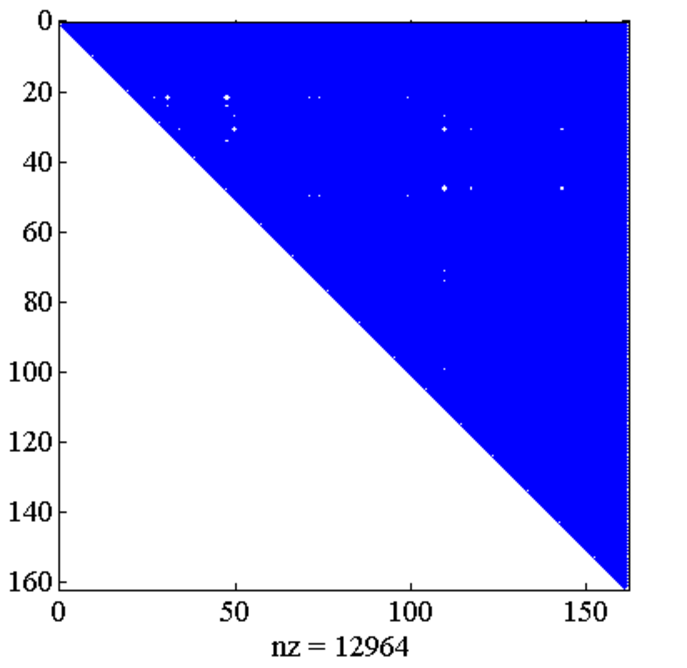
\includegraphics[width=5cm]{DDSchurMatS}
\caption{Upper triangular part of the Schur complement matrix.}
\label{fig:DDSchurMatS}
\end{figure}

\begin{figure}[ht!]
\centering
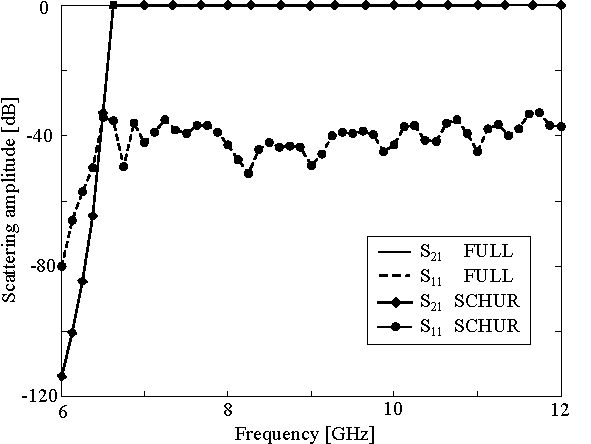
\includegraphics[width=10cm]{WRfreqSchur}
\caption{Frequency response of the WR-90 waveguide segment computed with the Schur complement algorithm.}
\label{fig:WRfreqSchur}
\end{figure}

\clearpage
\subsubsection{FETI-DP analysis}

We proceed with the analysis employing the FETI-DP algorithm in his version restricted to dual-primal unknowns. The global matrix, assembled as a whole for Fig. \ref{fig:DDFETIMat}, is composed of a block-diagonal part which is symmetric and and non-symmetric off-diagonal blocks parts.

\begin{figure}[ht!]
\centering
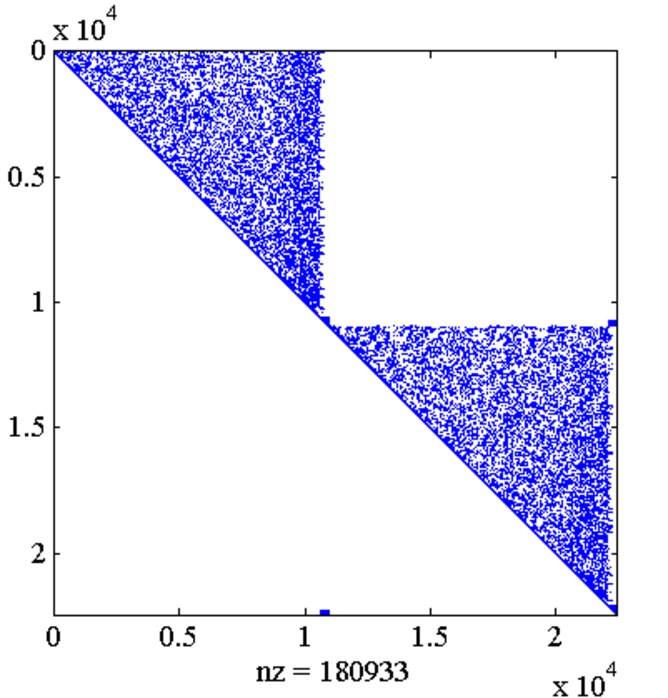
\includegraphics[width=10cm]{DDFETIMat}
\caption{FETI-DP based domain decomposition global system matrix. The upper triangular part of the symmetric blocks are  shown to enhance visibility of these parts. }
\label{fig:DDFETIMat}
\end{figure}

The first test is performed exciting the structure with DOM at 10~GHz. The convergence history in the relative error between successive approximations of the dual-primal unknowns on the boundary is shown in Fig. \ref{fig:Convergence}. The algorithm required in the average 430 iterations ($\approx 200~\mathrm{s}$) to achieve an error of $10^{-2}$. The spectral response, when dominant mode boundary condition on waveports is used, is depicted in Fig. \ref{fig:WRfreqFETI}. An average Euclidean error on the spectrum is of 2.1~\%.

The poor convergence behavior is due to a non-optimal residual minimization. This result has motivated the use of the FETI-DP as a preconditioner for Krylov iterative solvers which not only guarantee the convergence of the solution, but somehow choose the best directions.


\begin{figure}[ht!]
\centering
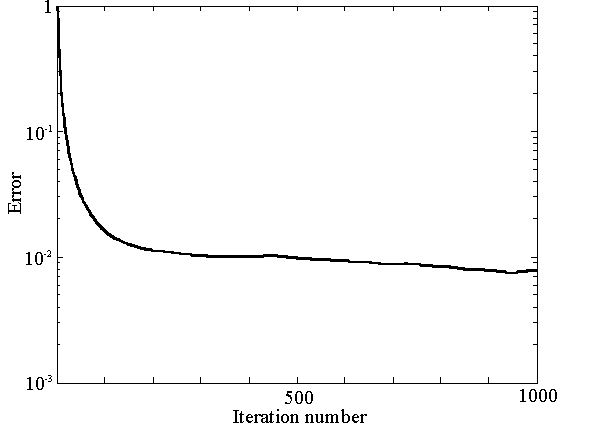
\includegraphics[width=10cm]{Convergence}
\caption{Convergence history of the restricted FETI-DP algorithm.}
\label{fig:Convergence}
\end{figure}

\begin{figure}[h!]
\centering
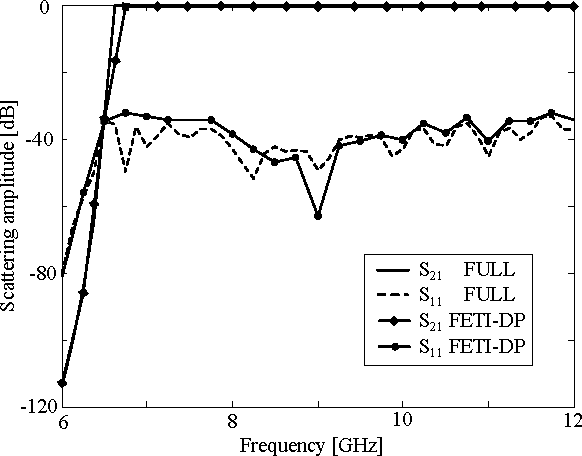
\includegraphics[width=10cm]{WRfreqFETI}
\caption{Comparison of the frequency response computed with direct full-domain solution and restricted FETI-DP (dominant mode waveports).}
\label{fig:WRfreqFETI}
\end{figure}
\clearpage

\subsection{\texorpdfstring{DD preconditioned GMRES($r$)}{DD preconditioned GMRES(r)}}

One of the main advantage of iterative solvers, when convergence is guaranteed, is the possibility to achieve approximate solutions within a prescribe tolerance. In many practical applications, the gaps between the CAD model, virtual, and the realized model are such that their electromagnetic behaviors differ of some \quotes{realization tolerances}. Hence, it may not be necessary to achieve numerical precision for acceptable simulation results. The numerical solution tolerance may be limited to one or a couple of magnitude orders lower to keep relatively good agreement with the real model.

Direct solvers might be used in single precision to decrease computational resources demand, but they still suffer from quadratic complexity for sparse matrices. One may also use an iterative solver, limiting the residual (error) norm to the desired tolerance. However the convergence speed, and hence the number of iterations and the overall computational times, tightly depend on the conditioning of the system matrix. It is also known that the conditioning gets worse as the problem gets larger. Adequate preconditioning of large problems matrices has to be performed in order to tackle iterative solutions in relatively acceptable amount of times. We will see that, due to block-matrix form of the domain decomposition systems, one can compute almost inexpensive very good preconditioners to tackle large problems.

\subsubsection{Performances of the various preconditioners}

To compare the performances of preconditioners, the WR-90 waveguide segment, partitioned in two subdomains as in Fig. \ref{fig:WR90Part}, have been analyzed at 10~GHz using double precision direct solvers to invert block-diagonal matrices. The results are compared with non-preconditioned full-domain solution. A restarting size of $r=100$ has been chosen and the residual error set to $10^{-12}$. 

\begin{figure}[h!]
\centering
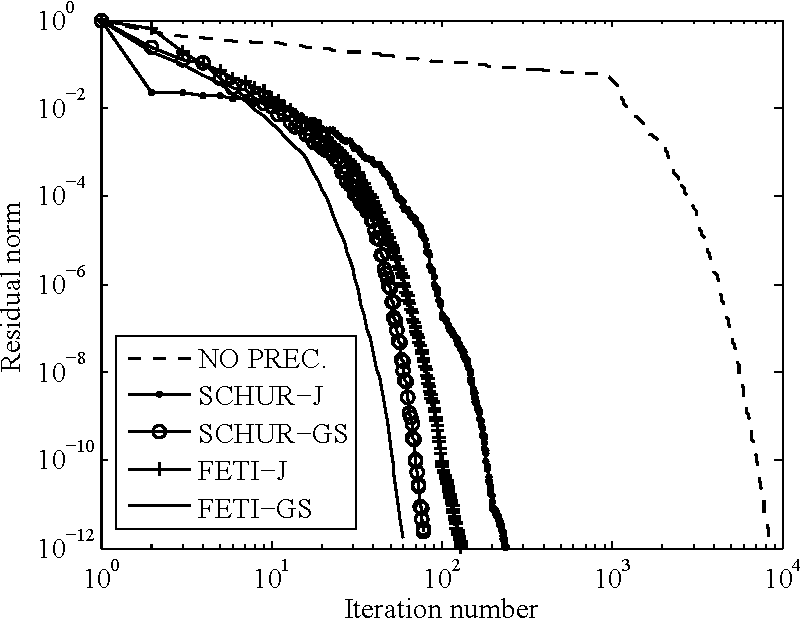
\includegraphics[width=10cm]{GMREScomp}
\caption{Comparison between the domain decomposition preconditioners and not preconditioned full-domain GMRES(100) solution.}
\label{fig:GMREScomp}
\end{figure}

Due to low residual error, all the simulation converge to the accuracy of a double precision sparse direct solution. This demonstrates that even the global FETI-DP problem is well posed and no energy is lost within interconnecting process (with only one interface). The effect of the restarting after 100 iterations can be appreciated on the DD-SCHUR Jacobi preconditioner run. In fact, after 100 and 200 iterations, the descent of the residual norm varies, leading for some iterations to a slower convergence.

\begin{table}[h!]
\begin{center}
\begin{tabular}{|c|c|c|c|}
\hline 
Solver & Iterations & Time & Peak memory \\ 
\hline
\hline 
Direct (double precision) & - & 1~s & 49.5~MB\\ \hline 
No preconditioner & 8459 & 276~s & 68.2~MB\\ \hline 
DD-Schur Jacobi precond. & 238 & 160~s & 68.6~MB\\ \hline 
DD-Schur Gauss-Seidel precond. & 78 & 54.5~s & 69.1~MB\\ \hline 
DD-FETI Jacobi precond. & 130 & 90~s & 69.7~MB\\ \hline 
DD-FETI Gauss-Seidel precond. & 58 & 41.8~s & 69.2~MB\\ \hline 
\end{tabular}
\end{center}
\caption{Times and memory requirements for different GMRES(100) runs at 10~GHz.}
\label{tab:gmresComp}
\end{table}

While the full-domain non preconditioned solution required about 276~s (8459 iterations), the domain decomposition preconditioners allowed to reduce the amount of times as shown in table \ref{tab:gmresComp}. The memory required by all the runs has been of about 69~MB, mainly allocated for the 100 orthonormal vectors (dense) used as Krylov space basis. In fact, all the assembled matrices required approximately 24~MB and the mesh about 10~MB.

It is clear that the Gauss-Seidel preconditioner leads to a better conditioning of the system matrix in both DD-SCHUR and DD-FETI cases. Let us analyze the performances of these solvers as the frequency of excitation varies (8, 10 and 12~GHz).

\begin{figure}[h!]
\centering
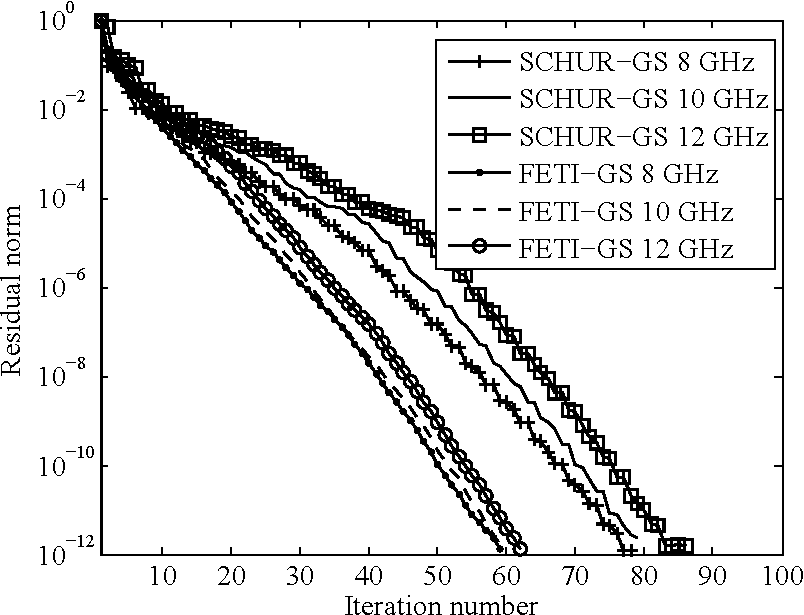
\includegraphics[width=10cm]{DDfreqComp}
\caption{Comparison between the SCHUR and FETI Gauss-Seidel preconditioned GMRES(100) runs as the frequency of excitation varies.}
\label{fig:DDfreqComp}
\end{figure}

As expected \cite{dyczij1999efficient}, the condition number of the system matrices grows with the frequency, resulting in more iterations (Fig. \ref{fig:DDfreqComp}). The FETI approach behaves clearly better that the SCHUR alternative. However, the SCHUR approach remains an invaluable method for arbitrary domain partitioning, as the transfinite element waveports boundary conditions (with better accuracy) can be straightforwardly implemented. In fact, waveports interfaces shared by multiple subdomains may lead to non strictly block-diagonal system matrices and hence worse performances.

\begin{figure}[h!]
\centering
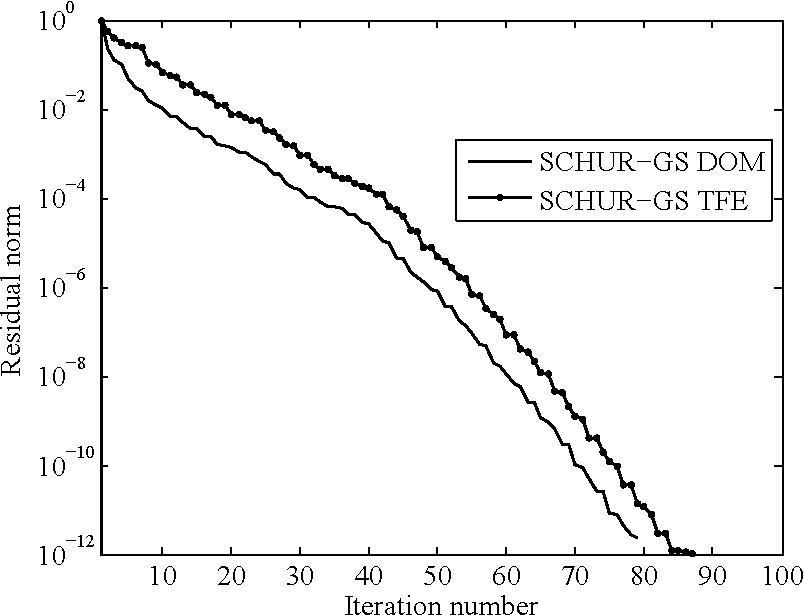
\includegraphics[width=10cm]{schurdomtfe}
\caption{Convergence history for SCHUR-GS GMRES(100) solution at 10~GHz with either dominant mode or transfinite element method waveports boundary conditions.}
\label{fig:schurdomtfe}
\end{figure}

In Fig. \ref{fig:schurdomtfe}, the convergence of both dominant mode and transfinite element waveports are shown. The higher accuracy of mode continuity is paid with a worse conditioning of the global DD-SCHUR system matrix.

As we are typically interested in error controlled solvers, we proceed evaluating the error induced in the scattering parameters while varying the maximum residual error. Several runs have been performed, considering dominant mode waveports boundary conditions at 10~GHz. Table \ref{tab:Sacc} shows that the FETI based method achieves faster a better overall accuracy than the Schur complement based. Also, while the scattering parameters error in the Schur complement based method might not be strictly lower than the prescribed residual error, in the case of the FETI they are.
However, when employing the transfinite element method on the waveports, the Schur complement based method behaves differently as shown in table \ref{tab:SaccTFE}, assuring an error lower than the prescribed residual error. 

\begin{sidewaystable}[h]
\begin{center}
\begin{tabular}{|c|c|c|c|c|}
\hline 
Solver & Residual error & $|S_{11}|$~[dB] & $|S_{21}|$~[dB] & $\frac{\Vert |S_\mathrm{ref}| - |S| \Vert_{2}}{\Vert|S_\mathrm{ref}|\Vert_2}$\\ 
\hline
\hline 
Direct (reference) & - & -42.8389 & -0.0024 & 0\\ \hline \hline
\setlength{\arrayrulewidth}{0.5pt}
DD-Schur Gauss-Seidel preconditioned & $10^{-2}$ & -26.7529 & -0.1958 & $2.23~10^{-2}$\\ \hline 
"& $10^{-4}$ & -42.5118 & -0.0030 & $1.4234~10^{-4}$\\ \hline 
"& $10^{-6}$ & -42.8397 & -0.0025 & $4.0786~10^{-7}$\\ \hline 
"& $10^{-8}$ & -42.8389 & -0.0024 & $3.4517~10^{-9}$\\ \hline 
"& $10^{-10}$ & -42.8389 & -0.0024 & $8.2561~10^{-11}$\\ \hline
"& $10^{-12}$ & -42.8389 & -0.0024 & $1.2571~10^{-13}$\\ \hline \hline
DD-FETI Gauss-Seidel preconditioned & $10^{-2}$ & -40.5331 & -0.0603 & $3.5~10^{-3}$\\ \hline 
"& $10^{-4}$ & -42.8404 & -0.0024 & $2.0280~10^{-6}$\\ \hline 
"& $10^{-6}$ & -42.8389 & -0.0024 & $1.1615~10^{-8}$\\ \hline 
"& $10^{-8}$ & -42.8389 & -0.0024 &  $5.5698~10^{-10}$\\ \hline 
"& $10^{-10}$ & -42.8389 & -0.0024 & $1.8771~10^{-12}$\\ \hline
"& $10^{-12}$ & -42.8389 & -0.0024 & $1.7357~10^{-14}$\\ \hline
\end{tabular}
\end{center}
\caption{Scattering parameters accuracy for different prescribed residual errors (runs at 10~GHz with dominant mode on waveports).}
\label{tab:Sacc}
\end{sidewaystable}

\begin{sidewaystable}[h]
\begin{center}
\begin{tabular}{|c|c|c|c|c|}
\hline 
Solver & Residual error & $|S_{11}|$~[dB] & $|S_{21}|$~[dB] & $\frac{\Vert |S_\mathrm{ref}| - |S| \Vert_{2}}{\Vert|S_\mathrm{ref}|\Vert_2}$\\ 
\hline
\hline 
Direct (reference) & - & -42.8035  & -0.0002 & 0\\ \hline \hline
\setlength{\arrayrulewidth}{0.5pt}
DD-Schur Gauss-Seidel preconditioned& $10^{-2}$ & -35.1814  & -0.0682 & $6.4~10^{-3}$\\ \hline 
"& $10^{-4}$ & -42.7897 &  -0.0002 & $6.8925~10^{-6}$\\ \hline 
"& $10^{-6}$ & -42.8034 &  -0.0002 & $1.3365~10^{-7}$\\ \hline 
"& $10^{-8}$ & -42.8035 &  -0.0002 & $3.9561~10^{-10}$\\ \hline
"& $10^{-10}$ & -42.8035 &  -0.0002 & $8.2355~10^{-12}$\\ \hline
"& $10^{-12}$ & -42.8035 &  -0.0002 & $2.0021~10^{-13}$\\ \hline
\end{tabular}
\end{center}
\caption{Scattering parameters accuracy for different prescribed residual errors (runs at 10~GHz with transfinite elements on waveports).}
\label{tab:SaccTFE}
\end{sidewaystable}

In the case of simply partitioned electromagnetic devices, the use of SCHUR-TFE (simply SCHUR) and FETI-DOM (simply FETI) might result to be reliable in the sense of the residual error. The first usually requires more iterations than the second (hence more time), but as it results from the formulation, should provide more accurate results, especially in multi-mode analyzes in which higher-order modes are excited.

\clearpage
\subsubsection{Performances against subdomains number}

We proceed analyzing the behavior of both SCHUR and FETI (with Gauss-Seidel preconditioners) while increasing the number of domains on the same mesh. A residual error of $10^{-4}$ can be retained, as it leads in both cases to a very good approximation of the solution. The whole waveguide is partitioned using Metis in 4, 8, 12 and 16 subdomains as depicted in Fig. \ref{fig:Partitions}. 

\begin{figure}[h!]
\centering
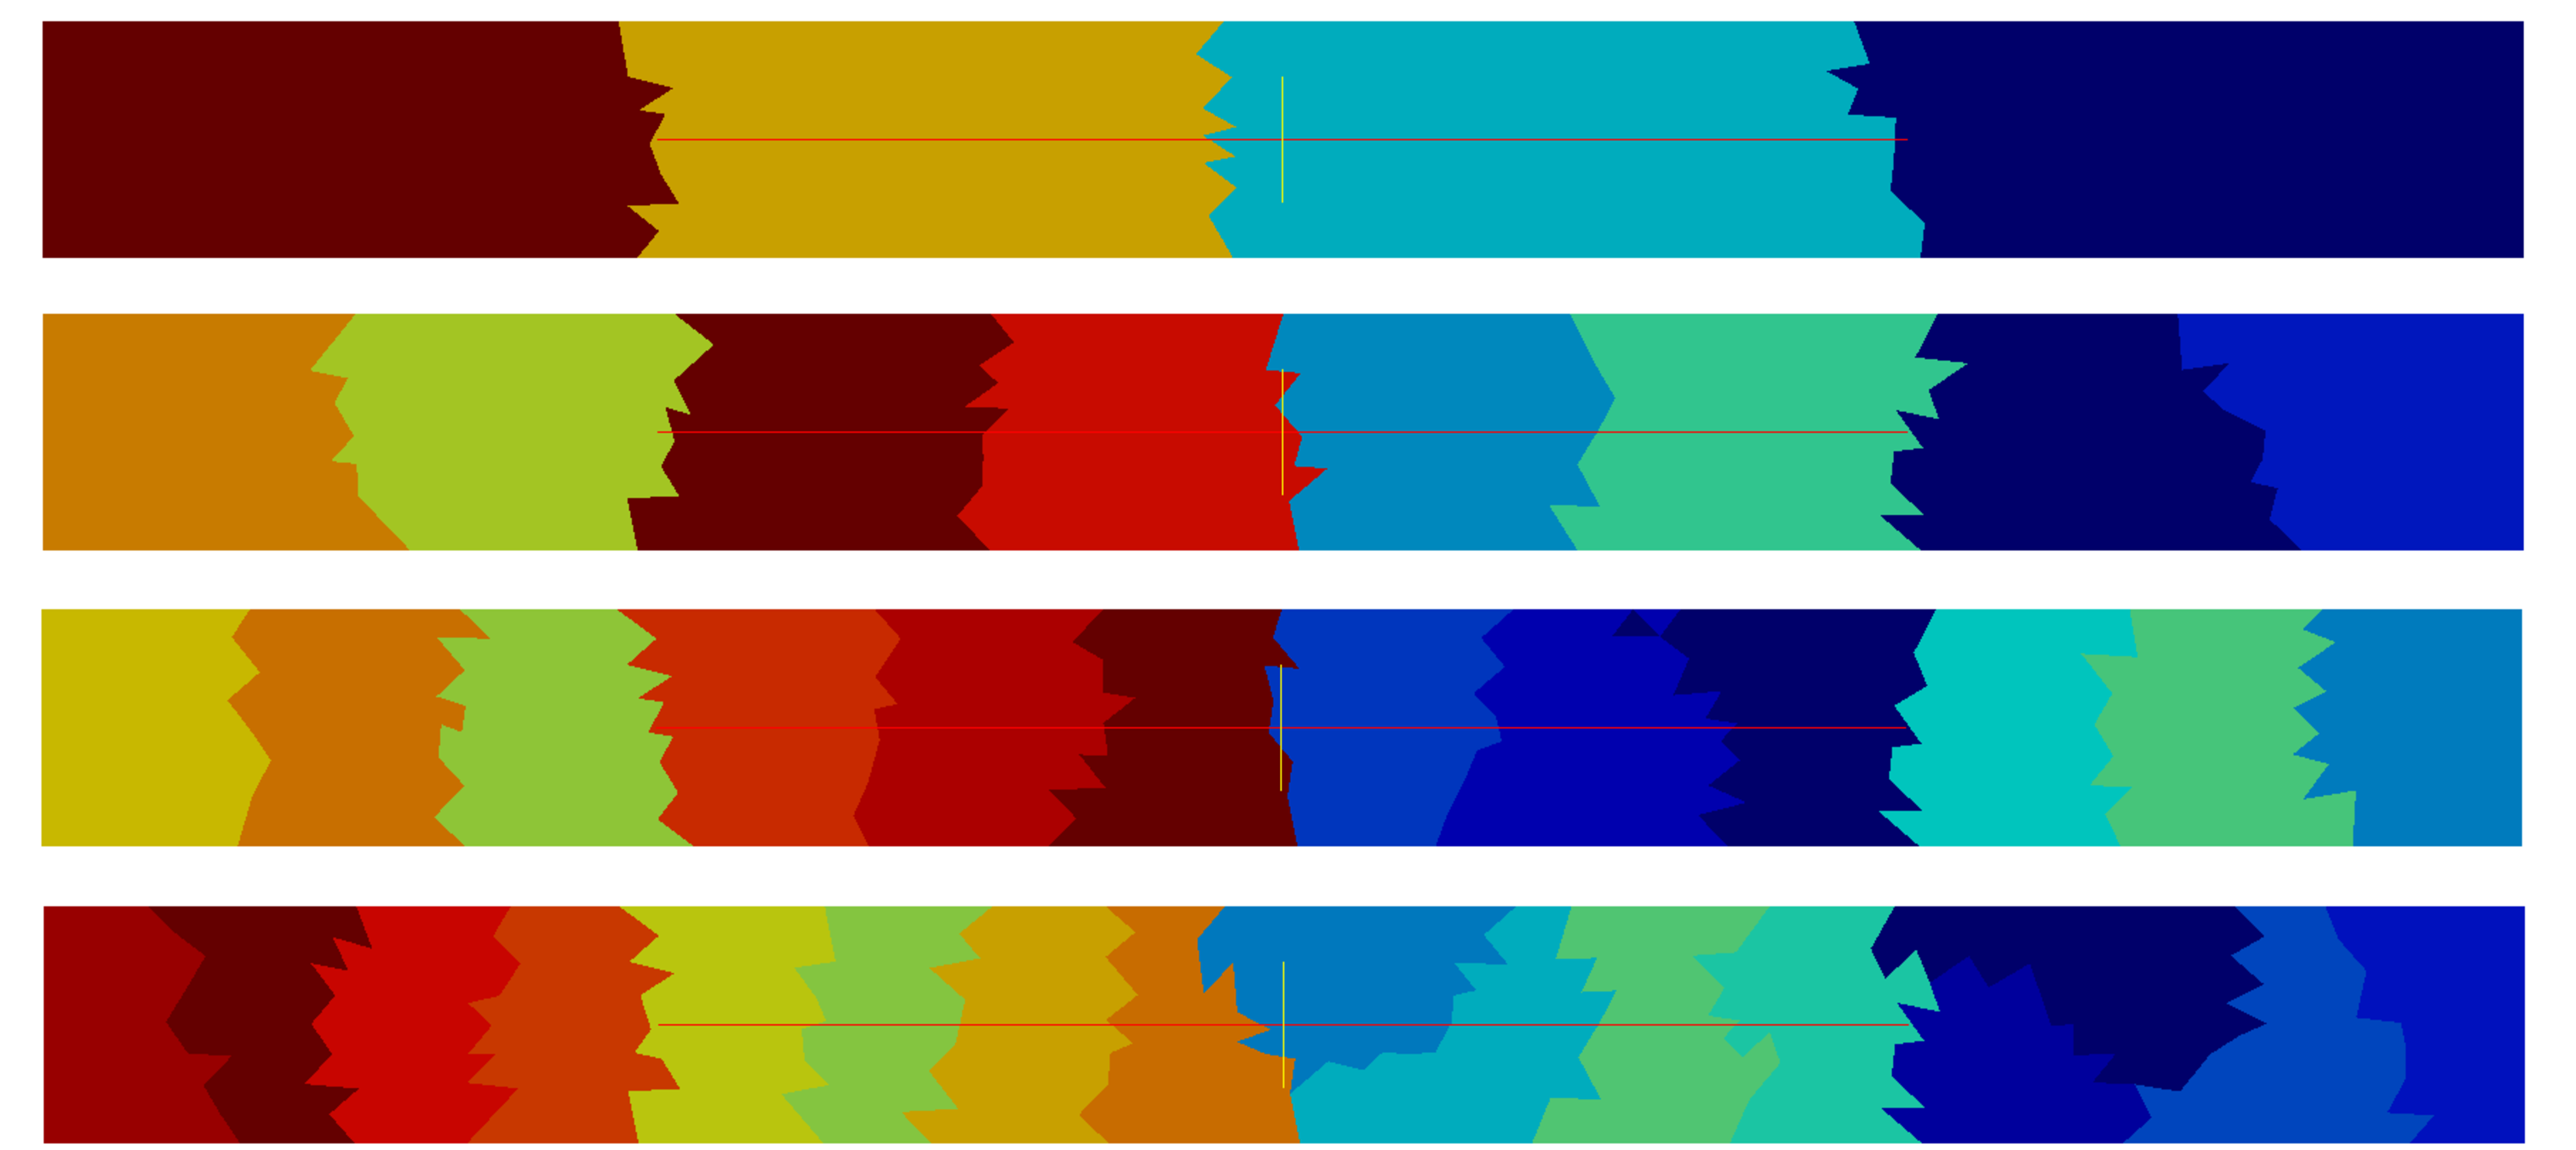
\includegraphics[width=13.4cm]{Partitions}
\caption{Rectangular waveguide partitionned in 4, 8, 12 and 16 subdomains with Metis.}
\label{fig:Partitions}
\end{figure}

The convergence histories for a 10~GHz excitations are shown in Fig. \ref{fig:DDsweep}. In the first three analyzes, an increase of the number of subdomains resulted in a slightly larger number of iterations to achieve the residual error for both solvers. In the case of 16 domains, the convergence resulted to be much harder to achieve, especially for FETI. Furthermore, in this case, the error on the scattering parameters resulted not to be bounded by the residual error as shown in table \ref{tab:SaccDDSweep}.

\begin{table}[h]
\begin{center}
\begin{tabular}{|c|c|c|}
\hline 
Solver (Nbr of Tetrahedra) & Nbr. of Sub-domains & $\frac{\Vert |S_\mathrm{ref}| - |S| \Vert_{2}}{\Vert|S_\mathrm{ref}|\Vert_2}$\\ 
\hline \hline 
\setlength{\arrayrulewidth}{0.5pt}
SCHUR (20~602) & 4 & $1.5926~10^{-6}$\\ \hline 
"& 8 & $5.95814~10^{-6}$\\ \hline 
"& 12 &  $3.29779~10^{-5}$\\ \hline 
"& 16 & $2.96923~10^{-4}$\\ \hline
FETI (20~602) & 4 & $2.14849~10^{-6}$\\ \hline 
"& 8  & $5.48124~10^{-6}$\\ \hline 
"& 12 & $1.02953~10^{-5}$\\ \hline 
"& 16 & $5.93607~10^{-3}$\\ \hline
SCHUR (25~093) & 16 & $8.29628~10^{-6}$\\ \hline 
FETI (25~093) & 16 & $1.90617~10^{-6}$\\ \hline 
\end{tabular}
\end{center}
\caption{Scattering parameters accuracy for different prescribed residual errors (runs at 10~GHz) when edge corners are avoided.}
\label{tab:SaccDDSweep}
\end{table}

The slower convergence is mainly associated to the fact there exist some edges of the mesh shared by multiple subdomains. In fact, slightly increasing the number of tetrahedra, from 20~602 to 25~093, and partitioning the new mesh in 16 subdomains without \quotes{edge corners} (Fig. \ref{fig:Partitions2}) has led to a significantly better behavior (Fig. \ref{fig:DD16ref}). Furthermore, the residual error bound could be projected, as empirically found in the previous analyzes, on the scattering parameters.

\begin{figure}[h!]
\centering
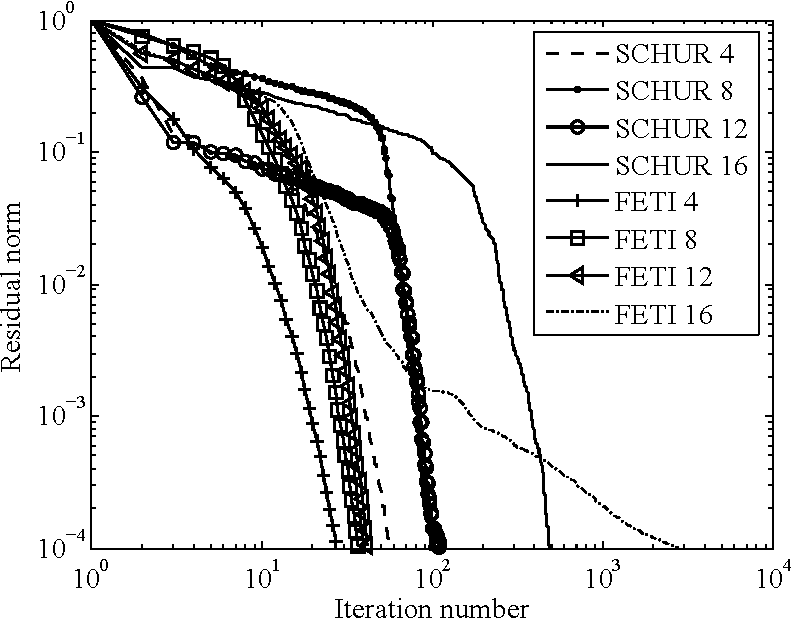
\includegraphics[width=10cm]{DDsweep}
\caption{Convergence histories for SCHUR and FETI GMRES(100) solvers as the number of subdomains is increased, respectively to TFE and DOM full analyzes at 10~GHz on relative mesh.}
\label{fig:DDsweep}
\end{figure}

\begin{figure}[h!]
\centering

\includegraphics[width=13.4cm]{Partitions2}
\caption{The two different meshes of the rectangular waveguide both partitioned in 16 subdomains. Top to bottom: 20~602 and 25~093 tetrahedra.}
\label{fig:Partitions2}
\end{figure}

\begin{figure}[h!]
\centering
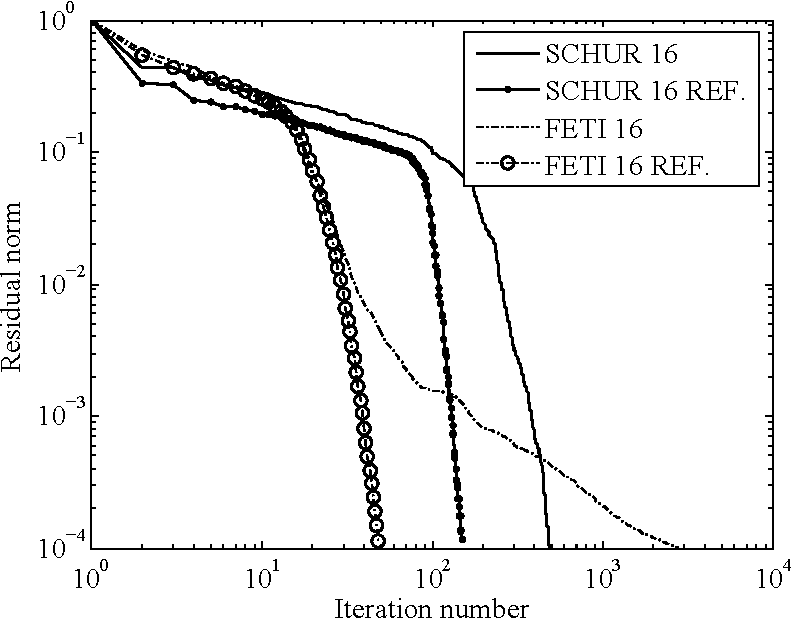
\includegraphics[width=10cm]{DD16ref}
\caption{Convergence histories for SCHUR and FETI GMRES(100) solvers on initial (20~602 tetrahedra) and refined (25~093 tetrahedra) meshes partitioned in 16 subdomains.}
\label{fig:DD16ref}
\end{figure}

In the average, increasing the number of subdomains on a given mesh leads to slower convergence. When partitioning the mesh, edge corners must be avoided for reliable analysis, until some solution is found to remove their bad contribution.

\subsubsection{Performances against problem size}

Although the electrical size remains the same (same structure at 10~GHz), let us analyze the performances of the solvers while increasing the mesh density and hence the number of unknowns, in order to evaluate their overall complexities. The simulations are run on a workstation equipped with an Intel Xeon CPU E5-1607 3~GHz 4 cores CPU and 64~GB of physical memory. The plots for several runs on the previous WR-90 waveguide are shown in Figs. \ref{fig:DirectCompl} and \ref{fig:IterCompl}.

\begin{figure}[h!]
\centering
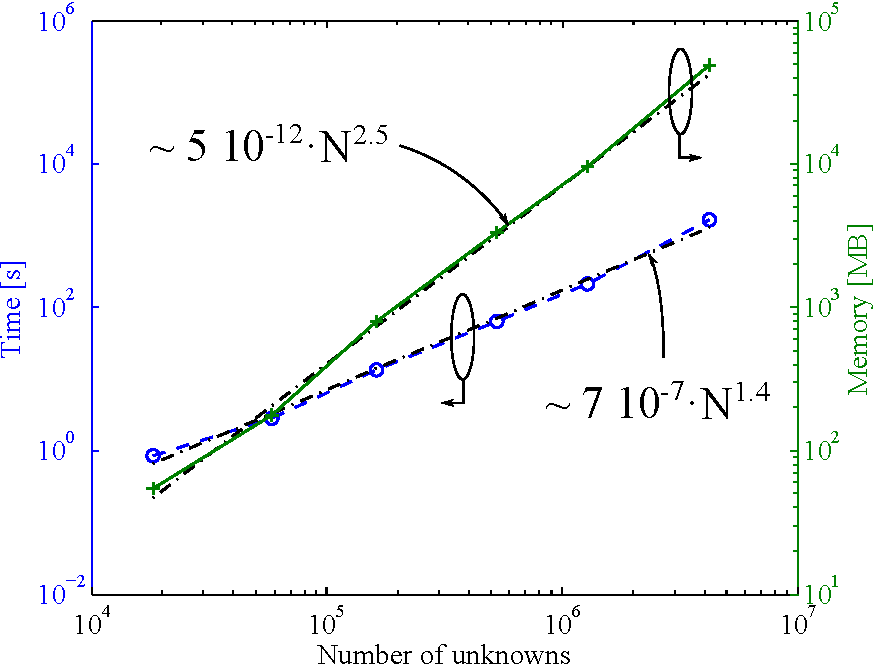
\includegraphics[width=10cm]{DirectCompl}
\caption{CPU time and memory consumption for different problem sizes analyzed with FES employing the double precision sparse direct solver.}
\label{fig:DirectCompl}
\end{figure}

\begin{figure}[h!]
\centering
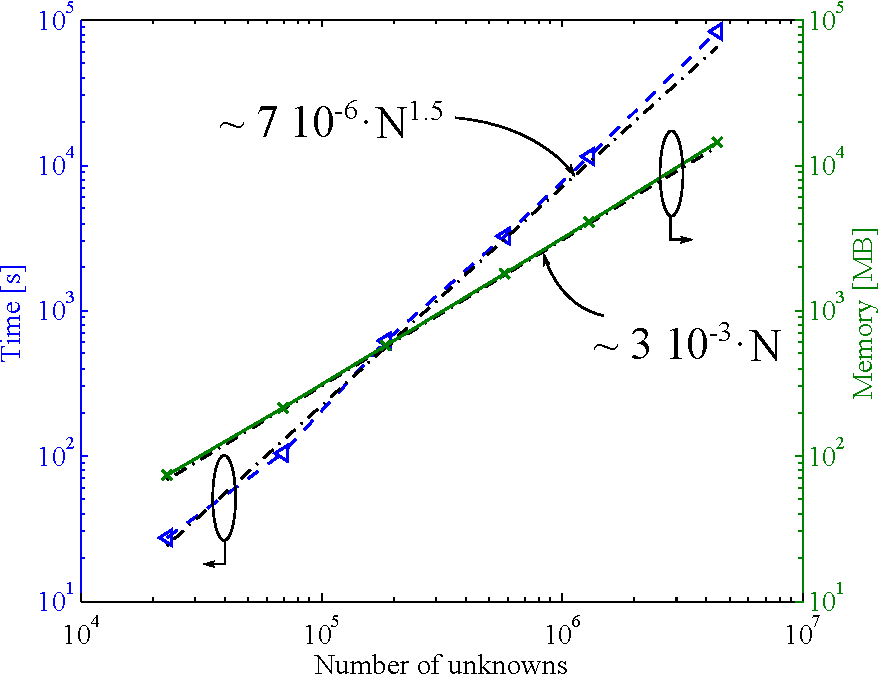
\includegraphics[width=10cm]{IterCompl}
\caption{CPU time and memory consumption for different problem sizes analyzed with FES employing the GMRES(100) FETI-DP preconditioned solver.}
\label{fig:IterCompl}
\end{figure}

The direct solver has a complexity of about $O(N^{2.5})$ in terms of memory, which agrees with what was stated in chapter \ref{chap:INT}, and the CPU times scale almost with an $O(N^{1.4})$ complexity. The GMRES(100) solver, FETI-DP preconditioned with the maximum number of partitions without edge corners formation and residual error of $10^{-4}$, fundamentally scales linearly in terms of memory ($O(N)$) and the times behave as $O(N^{1.5})$. It is worth noticing that while the direct solver totally exploits all the 4 cores of the CPU on which the simulations are run, the GMRES does not totally and only the sequential preconditioning does on each subdomain. Also, in the last simulation of 4.3 millions of unknowns, the direct solver required 48~GB of memory while the iterative solver on 14~GB, and hence a four times larger problem (16 millions of unknowns) could be solved on the same workstation.

%\subsection{Frequency selective radome-enclosed patch antennas array}
%
%
%In this last test we analyze the case of an large antenna problem to evaluate the influence of the residual error truncation on the antenna parameters.
%The structure analyzed is depicted in Fig. \ref{fig:RadomeFSS}. It consists of 14 2.45~GHz coaxial fed circular patch antennas \cite{maddio2011new} disposed on a 1.6~mm-thick FR4-epoxy disc substrate ($\epsilon_r = 4.4$, $\mu_r = 1$ and $\tan \delta = 0.02$) with 225~mm of diameter ($\approx 1.84~\lambda_0$). All metallic parts are considered perfect electric conductors. The enclosing radome is composed of an half sphere shell 2~mm-thick plexiglass substrate ($\epsilon_r = 3.4$, $\mu_r = 1$ and $\tan \delta = 0.001$) on which metallic O-rings (inner diameter of 4.2~mm and outer of 10~mm) are imprinted. The radome has me
%
%\begin{figure}[!]
%\centering
%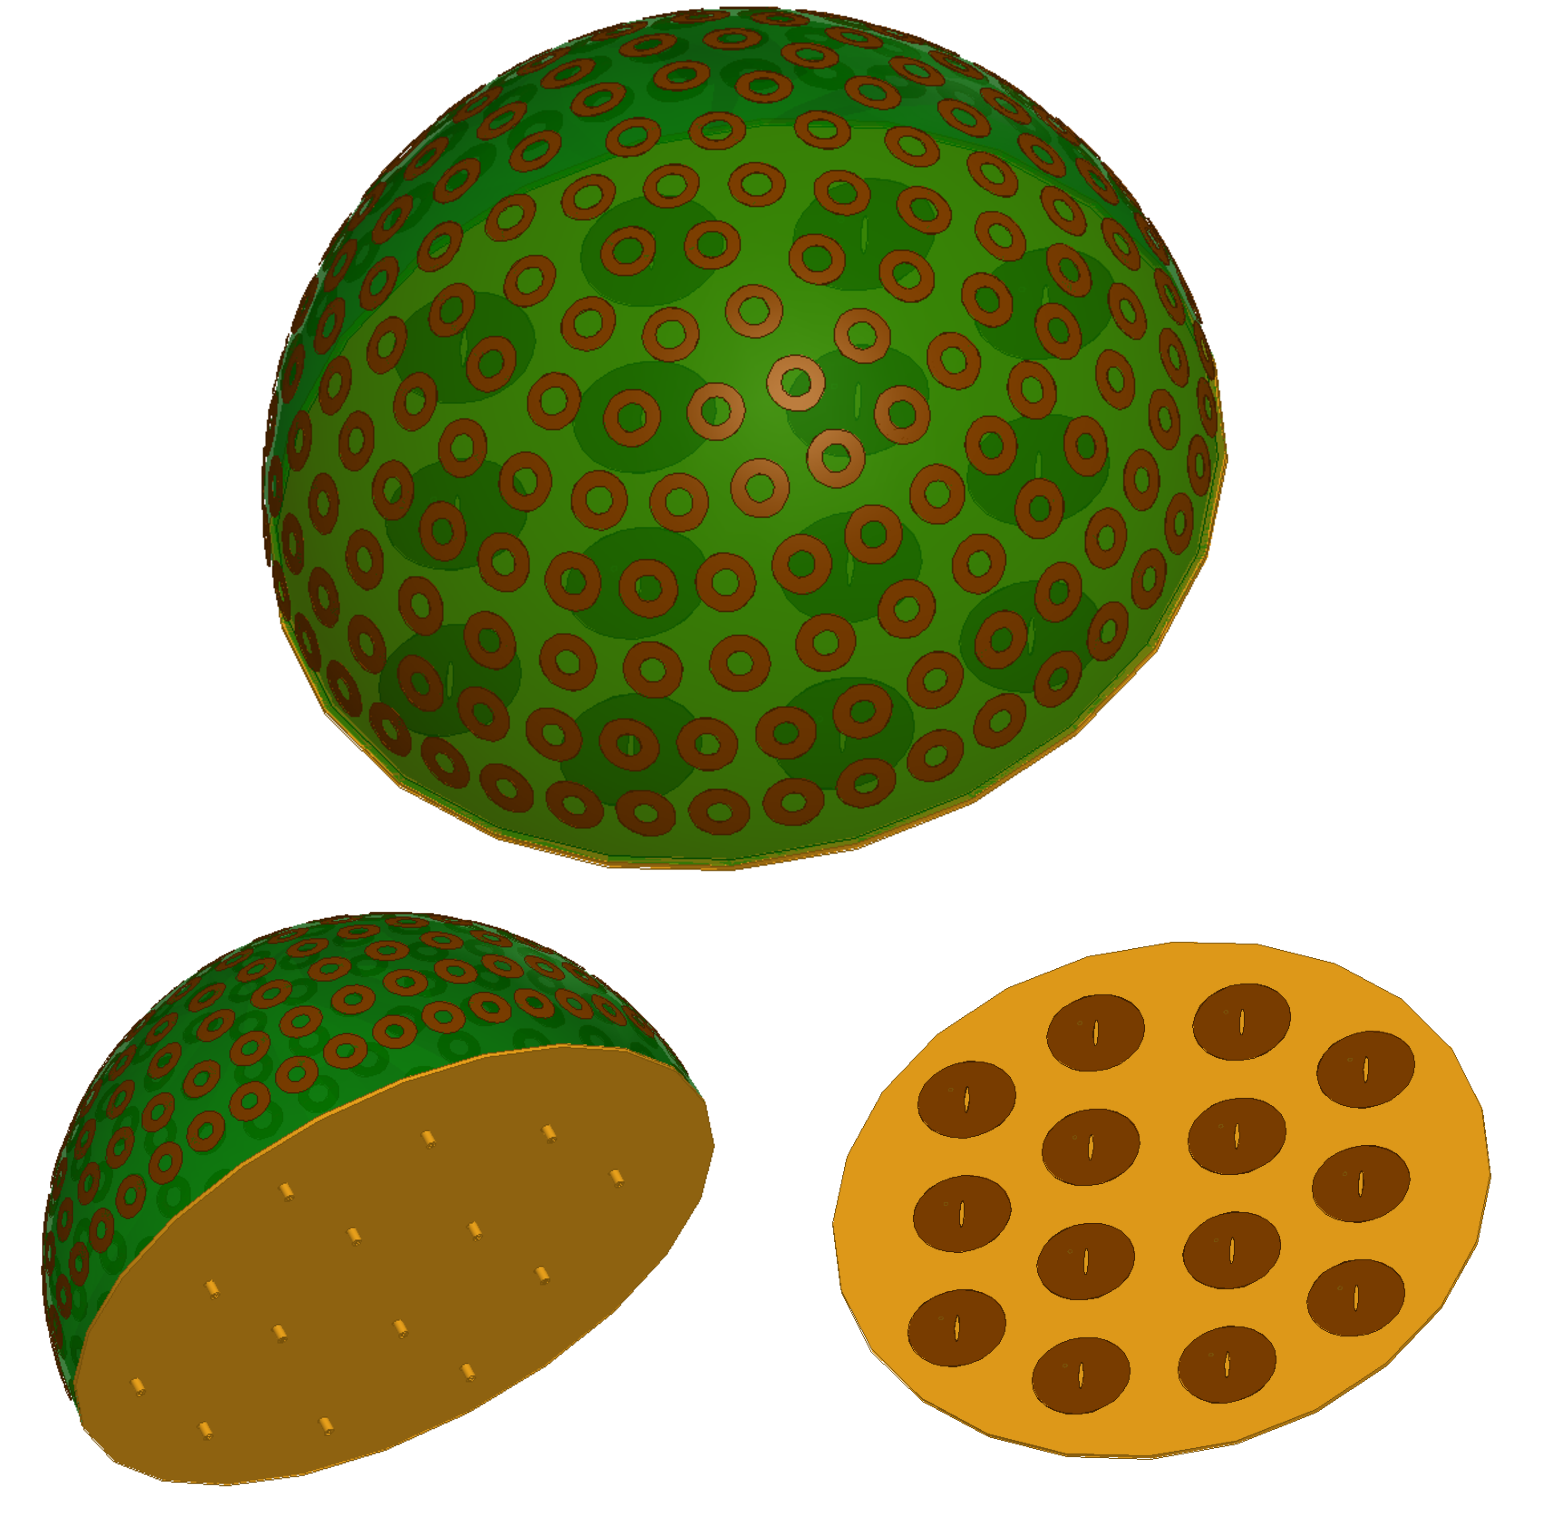
\includegraphics[width=13.4cm]{RadomeFSS}
%\caption{CAD model of the FSS radome-enclosed circular patch antenna array.}
%\label{fig:RadomeFSS}
%\end{figure}
%
%The mesh of the structure has led to almost 1~255~428 tetrahedra due to the small thicknesses of the substrate and the radome, Also, around metals the mesh density had to be increased in order to accurately approximate the large fields gradients (Fig. \ref{fig:Mesh}).
%
%\begin{figure}[!]
%\centering
%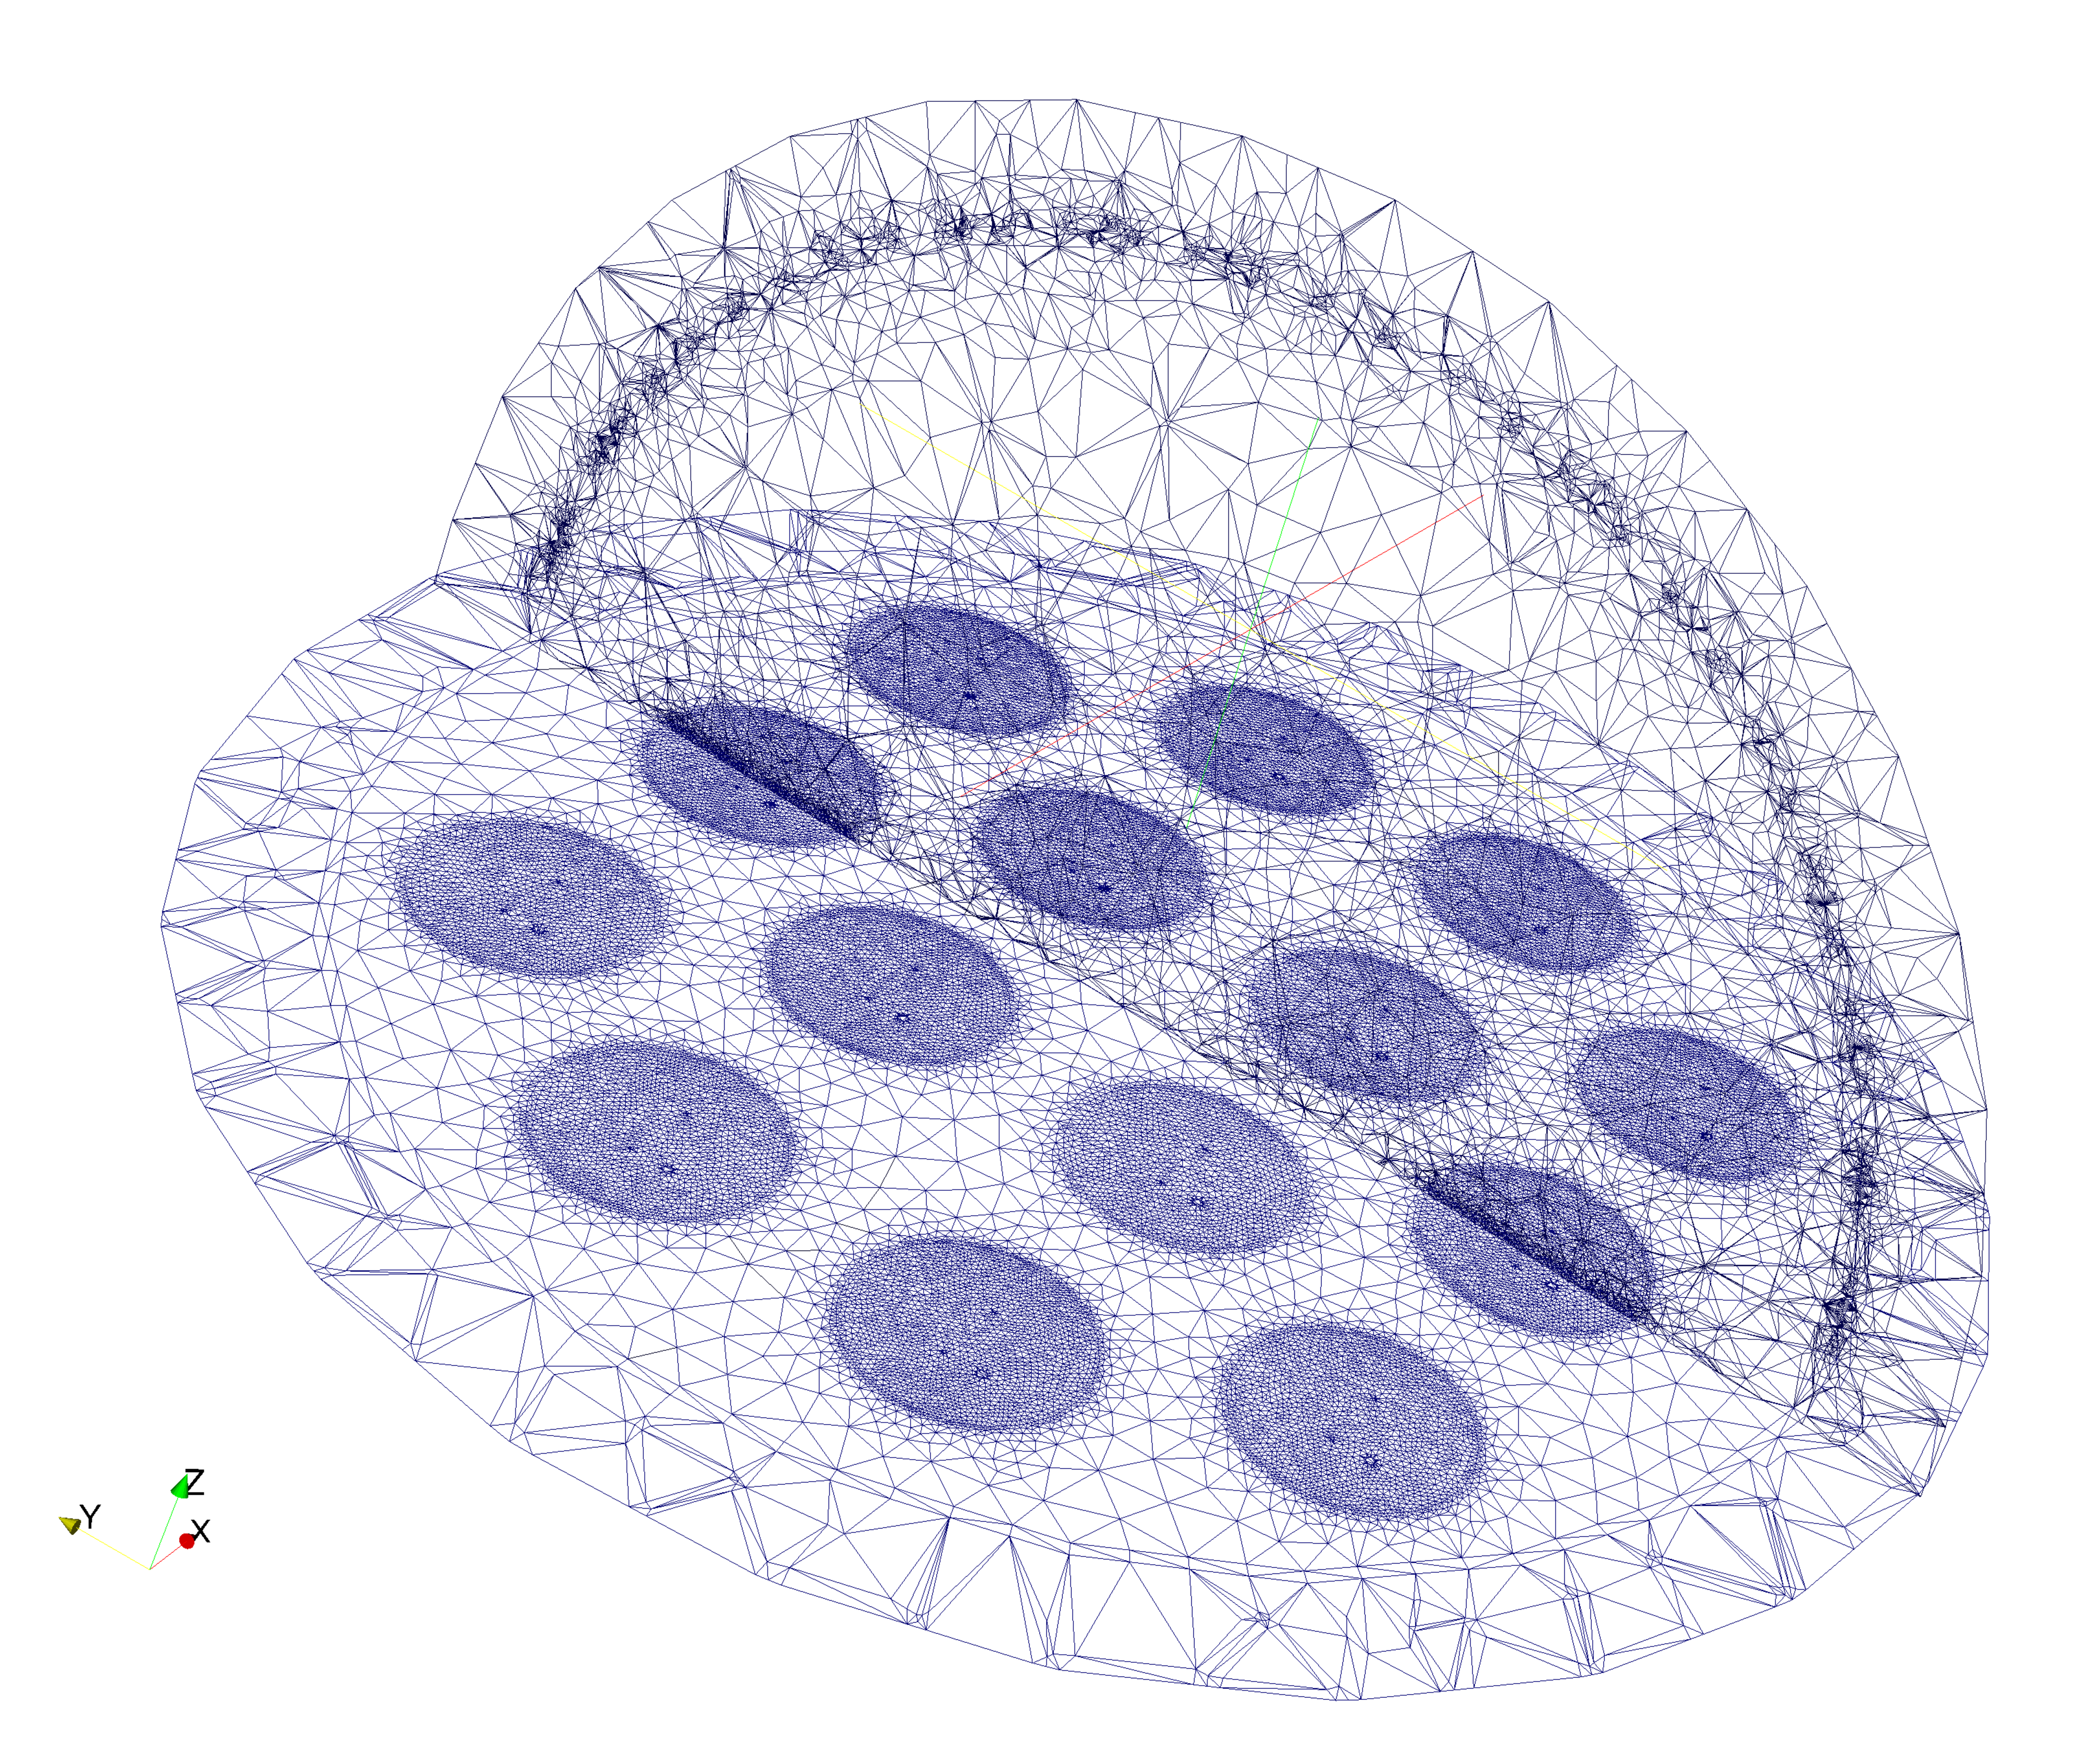
\includegraphics[width=13.4cm]{Mesh}
%\caption{Cross sections of the mesh.}
%\label{fig:Mesh}
%\end{figure}
%
%An assembly of the finite element matrices with first order curl-conforming basis functions and  has led to 1~297~027 unknowns, considering dominant, coaxial TEM mode impinging on each waveport. The radiation boundaries are located $\frac{\lambda_0}{4}$ away form the radome, on a concentric spherical shell.

\thispagestyle{empty}
\cleardoublepage
% !TEX root = ln_diss.tex
\graphicspath{{img/ch3/}}
\chapter[Nonlinear analysis]{Nonlinear Analysis of Passive Microwave Devices} \label{chap:NL}

It is well known that time-domain analysis of microwave devices including nonlinear materials often results to be computationally prohibitive when steady state fields are sought for \cite{deGersem2001}. A time-harmonic finite element (FE) approach at a single frequency is not sufficient to include all relevant phenomena. Higher-order harmonics are needed and may be taken into account, by using the harmonic balance finite element (HBFE) method \cite{yamada1988harmonic, yamada1989harmonic, yamada1991calculation}, also known as multiharmonic finite element method \cite{copeland2010domain, kolmbauer2012frequency}, which have demonstrated to provide a fast and accurate solution for low frequency, magneto-quasi-static problems.

In this chapter, the formulation of the HBFE is applied, for the first time, to the wave equation \cite{ntibarikure2012efficient, ntibarikure2014harmonic}. Several test cases will be shown, demonstrating the capabilities of the method for high frequency problems. Also, as some 3D problems have been reconducted to their 2D case with some restricting assumptions. The relative formulations will be presented.


%In this framework an algebraic domain decomposition (DD) technique was proposed to improve computational timings also in high frequency problems \cite{Guarnieri2010}, but no harmonic balance was present there and hence only the fundamental frequency was evaluated. In this letter, \cite{Guarnieri2010} is expanded by implementing a full harmonic balance domain decomposition finite element (HBDDFE) method for solving Helmholtz equation. The capability and efficiency of the method are proved on a waveguide filter example.

%%%%%%%%%%%%%%%%%%%%%%%%%%%%%%%%%%%%%%%%%%%%%%%%%%%%%%%%%%%%%%%%%%%%%%%%%%%%%%%%%%%%%
\section{Harmonic balance finite elements for the wave equation}
\label{sec:formulation}


\begin{figure}[!ht]
\centering
\includegraphics[width=10cm]{geometryLarge}
\caption{Generic multiport device where the total domain $\Omega$ is subdivided into linear subdomain $\Omega_1$ and a nonlinear subdomain $\Omega_2$.}
\label{fig:geometry}
\end{figure}

Given a generic multiport device (Fig.~\ref{fig:geometry}), its
domain $\Omega$, with boundary $\Gamma$, can be divided into a part $\Omega_1$ comprising only linear media, and another part $\Omega_2$ comprising all nonlinear media, with $\Omega = \Omega_1 \cup \Omega_2$ and
$\Omega_1 \cap \Omega_2 = \emptyset$.

The permittivity, the inverse of the permeability, that is the reluctivity, and the conductivity in $\Omega$ can be expressed as 
%
\begin{gather}
\epsilon_r(\mathbf{E}(\mathbf{r}),\mathbf{r}) = 
\begin{cases}
\bar{\epsilon}_r(\mathbf{r}), & \mathbf{r} \in \Omega_1,  \\
\tilde{\epsilon}_r(\mathbf{E}(\mathbf{r}), \mathbf{r}) \!=\!
\bar{\epsilon}_r(\mathbf{r}) \!+\! \mathcal{N}_\epsilon(\mathbf{E}(\mathbf{r})), & \mathbf{r} \in
\Omega_2,
\end{cases} \label{eq:epsnl}\\
\mu_r^{-1}(\mathbf{H}(\mathbf{r}),\mathbf{r}) = \nu_r(\mathbf{H}(\mathbf{r}),\mathbf{r}) = 
\begin{cases}
\bar{\nu}_r(\mathbf{r}), & \mathbf{r} \in \Omega_1, \\
\tilde{\nu}_r(\mathbf{H}(\mathbf{r}), \mathbf{r}) \!=\!
\bar{\nu}_r(\mathbf{r}) \!+\! \mathcal{N}_\nu(\mathbf{H}(\mathbf{r})), & \mathbf{r} \in
\Omega_2,
\end{cases}\label{eq:munl}\\
\sigma(\mathbf{E}(\mathbf{r}),\mathbf{r}) = 
\begin{cases}
\bar{\sigma}(\mathbf{r}), & \mathbf{r} \in \Omega_1, \\
\tilde{\sigma}(\mathbf{E}(\mathbf{r}), \mathbf{r}) \!=\!
\bar{\sigma}(\mathbf{r}) \!+\! \mathcal{N}_\sigma(\mathbf{E}(\mathbf{r})), & \mathbf{r} \in
\Omega_2,
\end{cases}\label{eq:signl}
\end{gather}

\noindent where $\mathbf{E}(\mathbf{r})$ is the electric field in the generic point
$\mathbf{r}$, $\mathbf{H}(\mathbf{r})$ is the magnetic field tightly bound to the electric field by \eqref{eq:waveeqErecH}. $\mathcal{N}_\times(\cdot)$ denotes a generic scalar operator describing the nonlinear behavior \cite{Guarnieri2010}. 

The electric field satisfies, within $\Omega$, the wave equation \eqref{eq:waveeqE}, here reported for convenience,
\begin{multline}
\nabla \times \nu_r(\mathbf{H}(\mathbf{r}),\mathbf{r}) \ \nabla \times {\mathbf{E}(\mathbf{r})} \ + j k_0 \zeta_0 \sigma(\mathbf{E}(\mathbf{r}),\mathbf{r}) \ {\mathbf{E}(\mathbf{r})} \ - k_0^2 \epsilon_r(\mathbf{E}(\mathbf{r}),\mathbf{r}) \ {\mathbf{E}(\mathbf{r})} = 0,\label{eq:waveeqEnl}
\end{multline}
\noindent where material properties are substituted by the relations \eqref{eq:epsnl}, \eqref{eq:munl} and \eqref{eq:signl}. The boundary conditions on $\Gamma$ can be any of those employed in chapter \ref{chap:FE}. For instance, in the following sections only transfinite elements will be employed on the waveports.
% $\Gamma_{12}$ corresponds to the internal boundary between subdomains $\Omega_1$ and $\Omega_2$.

The Galerkin framework applied to the problem leads to (see chapter \ref{chap:FE}) 
%
\begin{multline}
\label{eq:FEMformnl}
\int_\Omega \nabla \times \mathbf{w}_i^*(\mathbf{r}) \cdot \nu_r(\mathbf{H}(\mathbf{r}),\mathbf{r}) \nabla \times \mathbf{E}(\mathbf{r}) \ d\Omega \ + \\
 \hspace{-5cm} j k_0 \zeta_0 \int_\Omega \mathbf{w}_i^*(\mathbf{r}) \cdot \sigma(\mathbf{E}(\mathbf{r}),\mathbf{r}) \ \mathbf{E}(\mathbf{r}) \ d\Omega \ - \\
 \hspace{-3cm} k_0^2 \int_\Omega \mathbf{w}_i^*(\mathbf{r}) \cdot \epsilon_r(\mathbf{E}(\mathbf{r}),\mathbf{r}) \ \mathbf{E}(\mathbf{r}) \ d\Omega \ = \\
\int_{\Gamma} \mathbf{w}_i^*(\mathbf{r})  \times \nu_r(\mathbf{H}(\mathbf{r}),\mathbf{r}) \nabla \times {\mathbf{E}}(\mathbf{r}) \cdot \hat{\mathbf{n}} \ d\Gamma, 
\quad \forall \mathbf{w}_i(\mathbf{r}) \in \mathcal{W}_E.
\end{multline}

The multiharmonic dependence in the HBFE method is introduced by approximating the time and space dependent electric field $\mathcalb{E}(\mathbf{r},t)$ as a finite sum of harmonic components \cite{bachinger2005numerical}
%
\begin{equation} \label{eq:field}
\hat{\mathcalb{E}}(\mathbf{r}, t) = \sum^P_{p=1} \left( \mathbf{E}_{p}^{(s)}(\mathbf{r}) \sin(p
\omega_0 t) + \mathbf{E}_p^{(c)}(\mathbf{r}) \cos(p \omega_0 t) \right)
\end{equation} 

\noindent where $\omega_0$ is the fundamental angular frequency and, here and in the following, the hat over a quantity denotes its approximated value given by
the truncated Fourier series. 
$\mathbf{E}_{p}^{(s)}(\mathbf{r})$ and $\mathbf{E}_{p}^{(c)}(\mathbf{r})$ are the spatial basis functions defined as
$$
\mathbf{E}_{p}^{(s)}(\mathbf{r}) := \sum_{j=1}^{N} x_j^{(s)} \mathbf{w}_j(\mathbf{r}), \qquad \mathbf{w}_j(\mathbf{r}) \in \mathcal{W}_E,
$$ and
$$
\mathbf{E}_{p}^{(c)}(\mathbf{r}) := \sum_{j=1}^{N} x_j^{(c)} \mathbf{w}_j(\mathbf{r}), \qquad \mathbf{w}_j(\mathbf{r}) \in \mathcal{W}_E.
$$
and they expand, as in the conventional single harmonic case the field at $p\omega_0$. Hence they must individually satisfy the wave equation with $k_0 \leftarrow pk_0$.

The material properties can also be approximated as a truncated Fourier series \cite{copeland2010domain}
%
\begin{multline} \label{eq:matfourier}
\hat{{\epsilon}}_r(\mathbf{E}(\mathbf{r}), \mathbf{r}, t) = {\epsilon}_{r_0}(\mathbf{E}(\mathbf{r}),\mathbf{r}) \ + \\
\sum^{G_\epsilon}_{g=1} {\epsilon}_{r_g}^{(s)}(\mathbf{E}(\mathbf{r}),\mathbf{r}) \sin(g \omega_0 t) + \ \\ \sum^{G_\epsilon}_{g=1}  {\epsilon}_{r_g}^{(c)}(\mathbf{E}(\mathbf{r}),\mathbf{r}) \cos(g \omega_0 t),
\end{multline} 
\begin{multline} 
\hat{{\nu}}_r(\mathbf{H}(\mathbf{r}), \mathbf{r}, t) = {\nu}_{r_0}(\mathbf{H}(\mathbf{r}),\mathbf{r}) \ + \\ \sum^{G_\nu}_{g=1}  {\nu}_{r_g}^{(s)}(\mathbf{H}(\mathbf{r}),\mathbf{r}) \sin(g \omega_0 t) \ + \\
 \sum^{G_\nu}_{g=1} {\nu}_{r_g}^{(c)}(\mathbf{H}(\mathbf{r}),\mathbf{r}) \cos(g \omega_0 t),
\end{multline} 
\begin{multline} 
\hat{{\sigma}}(\mathbf{E}(\mathbf{r}), \mathbf{r}, t) = {\sigma}_{0}(\mathbf{E}(\mathbf{r}),\mathbf{r}) \ + \\
\sum^{G_\sigma}_{g=1} {\sigma}_{g}^{(s)}(\mathbf{E}(\mathbf{r}),\mathbf{r}) \sin(g \omega_0 t) \ + \\
\sum^{G_\sigma}_{g=1} {\sigma}_{g}^{(c)} (\mathbf{E}(\mathbf{r}),\mathbf{r}) \cos(g \omega_0 t),
\end{multline}
where the coefficients of the expansions are given by
\begin{equation}
\left\{
\begin{aligned} \label{eq:epsCoeffs}
{\epsilon}_{r_{0}}(\mathbf{E}(\mathbf{r}),\mathbf{r}) &= \frac{\omega_0}{2\pi}\int_0^{\frac{2\pi}{\omega_0}}
{\epsilon}_r(\mathbf{E}(\mathbf{r}),\mathbf{r}) \ dt, \\[.5cm]
{\epsilon}_{r_{g}}^{(s)}(\mathbf{E}(\mathbf{r}),\mathbf{r}) &=  \frac{\omega_0}{\pi}\int_0^{\frac{2\pi}{\omega_0}}
{\epsilon}_r(\mathbf{E}(\mathbf{r}),\mathbf{r}) \ \sin(g \omega_0 t) \ dt, \\[.5cm]
{\epsilon}_{r_{g}}^{(c)}(\mathbf{E}(\mathbf{r}),\mathbf{r}) &=  \frac{\omega_0}{\pi}\int_0^{\frac{2\pi}{\omega_0}} 
{\epsilon}_r(\mathbf{E}(\mathbf{r}),\mathbf{r}) \ \cos(g \omega_0 t) \ dt,
\end{aligned}
\right.
\end{equation}
\begin{equation}
\left\{
\begin{aligned} \label{eq:nuCoeffs}
{\nu}_{r_{0}}(\mathbf{H}(\mathbf{r}),\mathbf{r}) &=  \frac{\omega_0}{2\pi}\int_0^{\frac{2\pi}{\omega_0}}
{\nu}_r(\mathbf{H}(\mathbf{r}),\mathbf{r}) \ dt, \\
{\nu}_{r_{g}}^{(s)}(\mathbf{H}(\mathbf{r}),\mathbf{r}) &=  \frac{\omega_0}{\pi}\int_0^{\frac{2\pi}{\omega_0}}
{\nu}_r(\mathbf{H}(\mathbf{r}),\mathbf{r}) \ \sin(g \omega_0 t) \ dt, \\ 
{\nu}_{r_{g}}^{(c)}(\mathbf{H}(\mathbf{r}),\mathbf{r}) &=  \frac{\omega_0}{\pi}\int_0^{\frac{2\pi}{\omega_0}} 
{\nu}_r(\mathbf{H}(\mathbf{r}),\mathbf{r}) \ \cos(g \omega_0 t) \ dt, 
\end{aligned}
\right.
\end{equation}
\begin{equation}
\left\{
\begin{aligned} \label{eq:sigCoeffs}
{\sigma}_{0}(\mathbf{E}(\mathbf{r}),\mathbf{r}) &=  \frac{\omega_0}{2\pi}\int_0^{\frac{2\pi}{\omega_0}}
{\sigma}(\mathbf{E}(\mathbf{r}),\mathbf{r}) \ dt, \\
{\sigma}_{{g}}^{(s)}(\mathbf{E}(\mathbf{r}),\mathbf{r}) &=  \frac{\omega_0}{\pi}\int_0^{\frac{2\pi}{\omega_0}}
{\sigma}(\mathbf{E}(\mathbf{r}),\mathbf{r}) \ \sin(g \omega_0 t) \ dt, \\ 
{\sigma}_{{g}}^{(c)}(\mathbf{E}(\mathbf{r}),\mathbf{r}) &=  \frac{\omega_0}{\pi}\int_0^{\frac{2\pi}{\omega_0}} 
{\sigma}(\mathbf{E}(\mathbf{r}),\mathbf{r}) \ \cos(g \omega_0 t) \ dt.
\end{aligned}
\right.
\end{equation}

The orders of the approximations $P$ and $G_\times$ reflects on the accuracy of the solution and hence must be chosen upon appropriate energy criterion, for example retaining the part of the spectrum that have more than a prescribed portion of spectral power.

A conventional Galerkin approach, discretization of \eqref{eq:FEMformnl} 
%via \eqref{e:femexpansion}
leads to a system in the form $\mat{A}\vect{x} = \vect{b}$ with $\mat{A} \in \mathbb{C}^{N \times N}$, $\vect{x}$ and $\vect{b} \in \mathbb{C}^{N}$ (chapter \ref{chap:FE}).

In an HBFE approach, the following substitutions are performed in \eqref{eq:FEMformnl} 
\begin{gather*}
 \mathbf{E}(\mathbf{r}) \longrightarrow \hat{\mathcalb{E}}(\mathbf{r}, t), \\
 \epsilon_r(\mathbf{E}(\mathbf{r}),\mathbf{r}) \longrightarrow \hat{\epsilon}_r(\mathbf{E}(\mathbf{r}),\mathbf{r}, t),\\
\nu_r(\mathbf{H}(\mathbf{r}),\mathbf{r}) \longrightarrow \hat{\nu}_r(\mathbf{H}(\mathbf{r}),\mathbf{r}, t),\\
\sigma(\mathbf{E}(\mathbf{r}),\mathbf{r}), \longrightarrow \hat{\sigma}(\mathbf{E}(\mathbf{r}),\mathbf{r}, t).
\end{gather*}
Then, upon performing further testing with weights $\sin(q \omega t)$ or $\cos(q \omega t)$, $q = 1 \dots P$, and integrating over the time period of the fundamental $\left [ 0,\frac{2\pi}{\omega} \right )$,  a large linear system is obtained which has formally the same structure as a conventional finite element system but multiple matrices $\mat{A}$ and vectors $ \vect{x}$ and $\vect{b}$ are assembled depending on the harmonic of testing. The final system matrix can hence be represented as
%
\begin{equation}\label{eq:HBfemmn}
\begin{bmatrix}
\mat{A}^{(1s1s)} & \mat{A}^{(1s1c)} & \ldots &  \mat{A}^{(1sPc)} \\
\mat{A}^{(1c1s)} & \mat{A}^{(1c1c)} & \ldots &  \mat{A}^{(1cPc)} \\
\vdots & \vdots & \ddots & \vdots \\
\mat{A}^{(Pc1s)} & \mat{A}^{(Pc1c)} & \ldots &  \mat{A}^{(PcPc)}
\end{bmatrix}
\begin{bmatrix}
\vect{x}^{(1s)} \\
\vect{x}^{(1c)} \\
\vdots \\
\vect{x}^{(Pc)}
\end{bmatrix}
=
\begin{bmatrix}
\vect{b}^{(1s)}\\
\vect{b}^{(1c)}\\
\vdots\\
\vect{b}^{(Pc)}
\end{bmatrix}.
\end{equation}

\noindent The superscripts $(q[s|c])$ and $(p[s|c])$ indicates that the corresponding
entry was computed by testing \eqref{eq:FEMformnl} with $[\sin(q \omega t) | \cos(q \omega t)]$ while the corresponding harmonic basis of \eqref{eq:field}
was $[\sin(p \omega t) | \cos(p \omega t)]$. Harmonic coupling, which clearly worsen the system matrix sparsity, only occurs within elements pertaining to nonlinear material solids, for instance, off-diagonal sub-matrices of \eqref{eq:HBfemmn} vanish within linear materials.

The nonlinearity is finally handled via a relaxed iteration. As a starting point a null electric field $\vect{x}^0$ is assumed, computing the pertinent system matrix $\mat{A_{([x]^0)}}$ and known term $\vect{b_{([x]^0)}}$ and solving the system $\mat{A_{([x]^0)}} \vect{x}^1 = \vect{b_{([x]^0)}}$. The newly computed field $\vect{x}^1$ can now be used to update system matrix and known term and perform the following relaxed iteration:
% %
\begin{equation} \label{eq:lastLinearSystem}
 \mat{A_{(\gamma \vect{x}^{i-1} + (1-\gamma) \vect{x}^{i-2})}} \vect{x}^{i} = \vect{b_{(\gamma \vect{x}^{i-1} + (1-\gamma) \vect{x}^{i-2})}},
\end{equation}

\noindent with $i \geq 2$ and $\gamma\in(0,1]$. $\gamma=1$ gives the standard Picard iteration \cite{Guarnieri2010}, while low $\gamma$ values damps the oscillations
which may arise with highly nonlinear materials or high intensity impressed
fields at the cost of a slower convergence \cite{Silvester1997}. The process 
is repeated until the relative error between the updated solution
and the previous one, in the sense of the Euclidean norm, is less than a
prescribed value $\tau$, that is
$$ \frac{\Vert\vect{x}^{i}-\vect{x}^{i-1} \Vert_2}{\Vert\vect{x}^{i}\Vert_2} < \tau.$$

\section{Harmonic testing generalities}

The multi-harmonic testing can straightforwardly exploit the orthogonality between sine and cosine function defined as
%
\begin{eqnarray*}
\frac{\omega_0}{\pi}\int_{0}^{\frac{2\pi}{\omega_0}} \cos(m \omega_0 t) \ \cos(n \omega_0 t) \ dt &= &\delta_{mn},\\
\frac{\omega_0}{\pi}\int_{0}^{\frac{2\pi}{\omega_0}} \sin(m \omega_0 t) \ \sin(n \omega_0 t) \ dt &= &\delta_{mn},\\
\frac{\omega_0}{\pi}\int_{0}^{\frac{2\pi}{\omega_0}} \sin(m \omega_0 t) \ \cos(n \omega_0 t) \ dt &= &0,
\end{eqnarray*}
%
\noindent and for the constant terms in materials characteristics we have
\begin{eqnarray*}
\frac{\omega_0}{2\pi}\int_{0}^{\frac{2\pi}{\omega_0}} \cos(n \omega_0 t) \ dt &= & 1,\\
\frac{\omega_0}{2\pi}\int_{0}^{\frac{2\pi}{\omega_0}} \sin(n \omega_0 t) \ dt &= & 1,
\end{eqnarray*}
%
\noindent where $m \neq 0$, $n \neq 0$ and $\delta_{mn}$ is the Kronecker delta. Once the material properties expansion coefficients are computed, it might seem that the testing of \eqref{eq:FEMformnl} on the time period involves more than two trigonometric functions. It is possible to compute such testing integrals simply upon exploiting the following relations between the products of trigonometric functions
\begin{gather}
\cos (m \omega t) \cos(n \omega t) = \frac{1}{2} \cos ((m-n) \omega t ) + \frac{1}{2}  \cos((m+n) \omega t), \\
\sin (m \omega t) \sin(n \omega t) = \frac{1}{2} \cos ((m-n) \omega t ) - \frac{1}{2}  \cos((m+n) \omega t), \\
\sin (m \omega t) \cos(n \omega t) = \frac{1}{2} \sin ((m-n) \omega t ) + \frac{1}{2}  \sin((m+n) \omega t),
\end{gather}
\noindent hence splitting them into integrals that involve only two trigonometric functions.

All the testings on material properties can be either precomputed analytically, up to some prescribed orders, or numerically by the use of the fast fourier transform (FFT) \cite{frigo2005design}. The FFT is an efficient algorithm that implements the discrete Fourier transform, defined as
\begin{equation}
X_q = \sum_{k=0}^{N-1} x_k \exp{-j \frac{2\pi}{N} k q}, \qquad q=0,1,\ldots,N-1.
\end{equation}
\noindent When $x_k$ is a sequence of $N$ samples of $\hat{\epsilon}_r(\mathbf{E}(\mathbf{r}),\mathbf{r}, t)$, $\hat{\nu}_r(\mathbf{H}(\mathbf{r}),\mathbf{r}, t)$ or $\hat{\sigma}(\mathbf{E}(\mathbf{r}),\mathbf{r}, t)$ within the period $[0, \frac{2\pi}{\omega_0})$, then $X_q$ correspond to the expansion coefficients at the given normalized frequencies $q = \frac{g \omega_0}{\omega_0}$. Of course, one must use Euler formulas 
\begin{gather}
\cos (nt) = \frac{\exp{jnt} + \exp{-jnt}}{2},\\
\sin (nt) = \frac{\exp{jnt} - \exp{-jnt}}{2j},\\
\exp {jnt} = \cos(nt) + j \sin(nt),
\end{gather}
\noindent before and after the FFT and changing the phase where necessary to recover the proper values.

As will be shown in the intermodulation products example, $p, q$ and $g$ do not necessarily need to be integers. In fact, when considering multiple signals feeding a nonlinear device, these generate higher-order harmonics at multiples of the sum or difference between the impinging signals frequencies. Hence, for the necessary computational accuracy, the largest sampling period has to be considered in an FFT testing algorithm, and this is given by the largest common divisor between all the impinging signals.

\section{Transverse magnetic field formulation}

Let us assume the electric field $\mathbf{E}$ to be only $\hat{\mathbf{z}}$-directed such that $\mathbf{E} = E_z \hat{\mathbf{z}}$. Both fields and material properties are assumed not to vary along the $\hat{\mathbf{z}}$ direction and hence $E_z = E_z(x,y)$ and the magnetic field will have only transverse components, that is $H_x(x,y)$ and $H_y(x,y)$. Then the wave equation 
$$\nabla \times \dyad{\nu}_r \ \nabla \times {\mathbf{E}} + j k_0 \zeta_0 \dyad{\sigma} \ {\mathbf{E}} - k_0^2 \dyad{\epsilon}_r \ {\mathbf{E}} = 0,$$
\noindent becomes
\begin{equation}
\label{eq:helmholtz}
\nabla \cdot \dyad{\nu}_r \ \nabla {E_z} - j k_0 \zeta_0 \dyad{\sigma} \ {E_z} + k_0^2 \dyad{\epsilon}_r \ {E_z} = 0.
\end{equation}
\noindent In fact, we have
$$\nabla \times \dyad{\nu}_r \nabla \times E_z \hat{\mathbf{z}} = \nabla \times  (-\hat{\mathbf{z}} \times \dyad{\nu}_r \nabla E_z), $$
\noindent and by the use of the relation \cite{van2007electromagnetic} $\nabla \times  (\hat{\mathbf{z}} \times \mathbf{v}) = \hat{\mathbf{z}} \nabla \cdot \mathbf{v} - \frac{\partial \mathbf{v}}{\partial z}$ and remembering that $E_z(x,y)$ is independent on the $z$ variable, we have
$$\nabla \times (-\hat{\mathbf{z}} \times \dyad{\nu}_r \nabla E_z) = -\hat{\mathbf{z}} \nabla \cdot \dyad{\nu}_r \nabla E_z - \underbrace{\frac{\partial \dyad{\nu}_r \nabla E_z}{\partial z}}_{= 0}.$$
\noindent Finally we achieve
$$
-\hat{\mathbf{z}} \nabla \cdot \dyad{\nu}_r \ \nabla {E_z} + j k_0 \zeta_0 \dyad{\sigma} \ {E_z \hat{\mathbf{z}}} - k_0^2 \dyad{\epsilon}_r \ {E_z \hat{\mathbf{z}}} = 0.
$$
\noindent which can be written as \eqref{eq:helmholtz} upon removing the $\hat{\mathbf{z}}$ and multiplying by $-1$ all the terms of the equation. The field $E_z$ can be expanded with scalar basis functions $\phi \in \mathcal{V}(\Omega_h) := \{ \phi \in  \} \subset \mathcal{H}^1(\Omega, \Gamma_E)$ such that
$$E_{z} = \sum_{j=1}^{N_z} x_{z,j} \phi_j.$$
\noindent Galerkin projection leads to the following weak form
\begin{multline}
\int_\Omega \nabla \phi_i^* \cdot \dyad{\nu}_r \ \nabla {E_z} \ d\Omega + j k_0 \zeta_0 \int_\Omega \phi_i^* \dyad{\sigma} \ {E_z} \ d\Omega \ - \ \\ k_0^2 \int_\Omega \phi_i^* \dyad{\epsilon}_r \ {E_z} d\Omega = \int_\Gamma \phi_i^* \dyad{\nu}_r \ \nabla {E_z} \cdot \hat{\mathbf{n}} \ d\Gamma.
\end{multline}
\noindent where the vector identity $A \nabla \cdot \mathbf{B} = \nabla \cdot (A \mathbf{B} ) - \nabla A \cdot \mathbf{B}$ and Gauss' theorem have been exploited \cite{van2007electromagnetic}. $\hat{\mathbf{n}}$ is the outwardly directed normal unit vector.

Due to the field homogeneity along the $\hat{\mathbf{z}}$ direction, only a few components of materials tensors will contribute to the equation, for instance
\begin{gather}
\dyad{\nu}_r = 
\begin{bmatrix}
\nu_{r,\mathbf{x}\mathbf{x}} & \nu_{r,\mathbf{x}\mathbf{y}}\\
\nu_{r,\mathbf{y}\mathbf{x}} & \nu_{r,\mathbf{y}\mathbf{y}}
\end{bmatrix} = \begin{bmatrix}
\mu_{r,\mathbf{x}\mathbf{x}} & \mu_{r,\mathbf{x}\mathbf{y}}\\
\mu_{r,\mathbf{y}\mathbf{x}} & \mu_{r,\mathbf{y}\mathbf{y}}
\end{bmatrix}^{-1},\\
\dyad{\sigma} = \sigma_{\mathbf{z}\mathbf{z}},\\
\dyad{\epsilon}_r = \epsilon_{r,\mathbf{z}\mathbf{z}}.
\end{gather}

All the considerations made in chapter \ref{chap:FE} can be applied on $\Gamma$ integrals upon imposing the previous condition on the electric field. In particular, we will consider the waveports segments of figure \ref{fig:geometry} (as in 2D problem) with impinging $\mathrm{TE}_{m0}$ modes with $m \in \mathbb{N}^+$, hence respecting the $\mathbf{E} = E_z \hat{\mathbf{z}}$ condition. Also here, the modal distributions can be computed either analytically \cite{pelosi2009quick} or numerically by solving the transverse-longitudinal eigenvalue one-dimensional problem analogously to what is done in chapter \ref{chap:FE} for a two-dimensional problem.

\section{Numerical tests}

Here follows three tests performed to illustrate the performances of the HBFE method for the wave equation.

\subsection{Millimeter-wave bandpass filter with nonlinear dielectrics}

\begin{figure}[ht!]
\centering
\includegraphics[width=13.4cm]{bilat}
\caption{Cross section (H-plane) of a passband filter realized
by placing on the E-plane a dielectric slab partially metalized on both sides
(slab is shown in light grey; metal strips - uniform along $y$ are shown as
thick black lines) in a WR6 rectangular waveguide. Measures are given in $\mu{m}$.}
\label{fig:bilat}
\end{figure}

The millimeter-wave passband filter in WR6 (1651x825.5~$\mu$m) rectangular 
waveguide, initially presented in chapter \ref{chap:FE} with a full-wave formulation is here analyzed with a transverse magnetic 2D formulation \cite{bui1984broad}. 
The filter, uniform along $y$ axis, is realized by placing on the E-plane a 
dielectric slab partially metalized on both sides as shown by the H-plane cross
section of Fig.~\ref{fig:bilat}. All conductors are considered perfect. $\mu_r = 1$ and $\sigma = 0$ everywhere in $\Omega$.
The dielectric, enclosed in $\Omega_2$, presents a Kerr-type nonlinearity of
such that \cite{Guarnieri2010}
%, Ma1997}
\begin{equation}
\tilde{\epsilon}_r(\vec{E}(\vec{r}), \vec{r}) = \bar{\epsilon}_r(\vec{r}) + 
\alpha_2 \ |\vec{E}(\vec{r})|^2, \qquad \vec{r} \in \Omega_2
\end{equation}
\noindent where $\bar{\epsilon}_r(\vec{r}) = 2.1$ and 
$\alpha_2~=~1.625~10^{-10}~{\frac{\mathrm{m}^2}{\mathrm{kV}^2}}$.
%is chosen as \cite{Ma1997}. 

The Kerr-like behavior of the permittivity induces the generation of odd order harmonics, thus 
even ones can been neglected. For the relaxed
iteration stop criterion, $\tau = 10^{-6}$ has been chosen.
The continuity of the field at the ports is imposed through a modal expansion 
exploiting only $\mathrm{TE}_{m0}$ modes, $m = 2n+1$, $n=1,\ldots,4$, even $m$
modes being absent for the E-plane symmetry of the filter.  
The excitation is a $\mathrm{TE}_{10}$ mode at fundamental frequency impinging at
Port 1 with maximum field amplitude $E_ i$. The 
waveguide discontinuity represented by the filter transfers power to higher order
modes, which may result to be guided at higher harmonic frequencies.
Furthermore, as a sinusoidal excitation is chosen, only $\sin(p \omega t)$ 
related coefficients are retained.
Due to H-plane uniformity, the problem can be treated as two-dimensional \cite{pelosi2009quick}.
First order nodal elements are used and the discretization leads to 2473
degrees of freedom, 80 of which belong to the nonlinear subdomain $\Omega_2$, 
314 to the boundaries and 2079 to the linear subdomain $\Omega_1$. Such a fine
discretization is necessary to obtain a good approximation of the field up to 
the $5^\mathrm{th}$ harmonic.
%
\begin{figure}[!ht]
\centering
\includegraphics[width=12cm]{spectrumNHarm}
\caption{$\mathrm{TE}_{10}$ spectral response for linear (top) and nonlinear 
(bottom) permittivity with $E_i = 10$~$\frac{\mathrm{kV}}{\mathrm{m}}$. The results are compared with Comsol
RF module linear and nonlinear solutions.}
\label{fig:spectrumNHarm}
\end{figure}

As a first analysis, the effect of the total number of harmonics $P$
retained on the filter's spectral response is investigated
(Fig.~\ref{fig:spectrumNHarm}). For an incident field amplitude $E_i = 10$~${\frac{\mathrm{kV}}{\mathrm{m}}}$, the Picard iteration proved to converge. Equal mesh and parameters have been used to conduct a \mbox{2D} finite element (single harmonic) analysis with Comsol RF Module \cite{ComsolRF}. Being the nonlinear loop tackled differently (Comsol uses Newton algorithm), perfect matching in the spectral response is not obtained as for the linear permittivity case ($\alpha_2 = 0$).
It is evident from Fig.~\ref{fig:spectrumNHarm} that including 
the $3^\mathrm{rd}$ harmonic is crucial for proper evaluation of the device
bandwidth.

The electric field distribution at 146~GHz, 438~GHz and 730~GHz are shown in Fig.~\ref{fig:Fields}. As higher-order harmonics are generated by the fundamental field flowing through nonlinear parts of the device, the related fields will be, also for passivity concerns, of various orders of magnitude lower.

\begin{figure}[!ht]
\centering
\includegraphics[width=13.4cm]{FieldsCol}
\caption{$|\mathrm{E}_y|$ distribution within the filter at fundamental 
($f_0 =$ 146 ~GHz), $3^\mathrm{rd}$ and $5^\mathrm{th}$ order harmonics 
($\mathrm{E_i = 10 ~{\frac{\mathrm{kV}}{\mathrm{m}}}}$).}
\label{fig:Fields}
\end{figure}

\begin{figure}[!ht]
\centering
\includegraphics[width=12cm]{spectrumS21b}
\caption{$|S_{21}|$ of the nonlinear filter for
several values of $E_i$ compared to the linear case. Field is approximated
up to the $5^\mathrm{th}$ harmonic.}
\label{fig:spectrum}
\end{figure}

To gain better insight, simulations have
been repeated with $E_i=5$~${\frac{\mathrm{kV}}{\mathrm{m}}}$ and $E_i=15$~${\frac{\mathrm{kV}}{\mathrm{m}}}$, for $P=5$. 
The results compared to those of a linear device are shown in Fig.~\ref{fig:spectrum}. 
There is an evident shift of the band 
towards lower frequencies as higher power densities are involved, which agrees 
to \cite{Yatsyk2006}. Furthermore the $E_i=15$~${\frac{\mathrm{kV}}{\mathrm{m}}}$ did not 
converge with Picard iteration and required a relaxed $\gamma = 0.1$ iteration.
% In this case, the abrupt variation of $|S_{21}|$ around $139.5$~GHz points out 
% that $P=5$ is not sufficient to accurately analyze the device.
% Indeed, the power associated to harmonics grows as the incident field 
% increases as shown in Fig.~\ref{fig:harmSpectrum}. 
% \st{but a finer mesh would be necessary to allow for higher $P$ values.}
% \begin{figure}[!t]
% \centering
% \includegraphics{harmSpectrum}
% \caption{Spectral responses at $3^\mathrm{rd}$ (top) and $5^\mathrm{th}$ 
% (bottom) harmonics
% for scattered modes (Incident $\mathrm{TE}_{10}$ with (a) $E_i = 10$~kV/m;
% (b) $E_i = 15$~kV/m.}
% \label{fig:harmSpectrum}
% \end{figure}

Analysis of the spectral response convergence is performed computing the relative
error, in Euclidean norm sense, all over the device bandwidth while increasing 
the order of HBFE system such that
\begin{equation} \label{eq:convError}
	\mathrm{error}(P=p) = \frac{\| |S_{21}|^{p} - |S_{21}|^{p-2}\|_2}
	{\| |S_{21}|^{p-2}\|_2} 
\end{equation}
\noindent with $p = 2n+1$, $n=1,\ldots,5$. Results (Fig.~\ref{fig:convergence})
show faster convergence for low intensity impinging fields.

\begin{figure}[!ht]
\centering
\includegraphics[width=12cm]{convergence}
\caption{
Relative error of the spectrum at fundamental frequency for various $E_i$ values.}
\label{fig:convergence}
\end{figure}

To enhance the computational efficiency, a Schur complement based domain decomposition approach is here proposed \cite{Guarnieri2010,Guarnieri2009}. The multiharmonic unknowns vector $[x]$ defined by the HBFE method over $\Omega$ can be split into two vectors $[x_{1}]$ and $[x_{2}]$ containing the unknowns belonging
to interior points in $\Omega_1$ and $\Omega_2$, respectively. Unknowns
belonging to the boundaries $\Gamma\cup\Gamma_{12}$ are placed in a third
vector $[x_{\Gamma}]$. The HBFE system can then be recast in :
%
\begin{equation}\label{eq:DD}
\begin{bmatrix}
 [A_{11}] &  0  &  [A_{1\Gamma_1}] \\
 0  &  [A_{22}]^{i-1} & [A_{2 \Gamma_2}]^{i-1} \\
 [A_{\Gamma_1 1}] & [A_{\Gamma_2 2}]^{i-1} & [A_{\Gamma \Gamma}]^{i-1}
\end{bmatrix}
\begin{bmatrix}
{[x_{1}]^{i}} \\
{[x_{2}]^{i}} \\
{[x_{\Gamma}]^{i}}
\end{bmatrix} 
=
\begin{bmatrix}
{[b_{1}]} \\
{[b_{2}]}^{i-1} \\
{[b_{\Gamma}]}^{i-1}
\end{bmatrix} 
\end{equation}

\noindent where $[A_{11}]$ contains the HBFE coefficients of the linear system
related to the unknowns $[x_{1}]$, with
null harmonic coupling coefficients, while $[A_{22}]$ contains coefficients for
the nonlinear subdomain $\Omega_2$. ${[A_{\Gamma_\times \times}]}$ and ${[A_{ \times \Gamma_\times}]}$
represent couplings between interior unknowns and 
boundary unknowns collected in $[x_\Gamma]$. 
By using the Schur complement concept, the boundary unknowns $[x_\Gamma]^{i}$ of
\eqref{eq:DD}, and hence the generalized scattering matrix of the device, can be retrieved \cite{Guarnieri2010, Guarnieri2009}.
Hence, in order to solve the HBDDFE system,
every single submatrix is assembled at first sight, then, within the iteration
loop, only the submatrices related to $\Omega_2$ and $\Gamma_{12}$ are to be
updated. The efficiency of this 
DD technique relies on the fragmentation of the
matrices and the subsequent computation of partial solutions. When the number
of coefficients related to the nonlinear media is small, noticeable
improvements can be achieved.

\begin{figure}[!ht]
\centering
\includegraphics[width=11cm]{acceleration}
\caption{Acceleration spectrum obtained for an HBFE system of several harmonic
orders. The computations are made for $E_i = 15$~${\frac{\mathrm{kV}}{\mathrm{m}}}$~($\gamma = 0.1$).}
\label{fig:acceleration}
\end{figure}

The efficiency of the DD technique can be
assessed by its acceleration,
$$\text{Acceleration} = \frac{\text{HBFE time}}{\text{HBDDFE time}},$$
\noindent that is the ratio between time for a full domain
computation - inclusive of nonlinear iterations - and the corresponding DD
computation (assembly and solve) \cite{Guarnieri2010}. Fig.~\ref{fig:acceleration} presents the acceleration for each frequency point, and for different values of $P$ at  $E_i = 10~{\frac{\mathrm{kV}}{\mathrm{m}}}$. 

In general, higher order HBDDFE systems have lower acceleration, since the
matrices dimensions related to nonlinear media increase. With a
$P=3$ system, the acceleration varies in the range [2.51,
9.15], averaging to 4.18, and leading to an HBDDFE solution in 24\% of the
time required by a full domain HBFE solution.

\subsection{Microwave circulator intermodulation products}


The test case of a H-plane circulator in rectangular waveguide constituted by a Y-junction with a magnetized ferrite post is presented \cite{koshiba1986finite}. The circulator comprises three WR90 (cross-section dimensions $a$=22.86~mm and $b$=10.16~mm) waveguide sections of length $l$=33.4~mm joined forming a 120\textdegree~angle one with each other in a Y shape and a magnetized ferrite post of height $b$, hence spanning the whole device height. The post is an equilateral triangular prism of base side $d$=7.80~mm, placed at the center of the junction as sketched in Fig. \ref{fig:Koshiba} and it is magnetized along $\hat{\mathbf{z}}$.

\begin{figure}[!ht]
\centering
\includegraphics[width=8cm]{Koshiba}
\caption{Geometry layout of the ferrite circulator. The two domains $\Omega_1$ and $\Omega_2$, respectively corresponding to linear and nonlinear domains, are shown.}
\label{fig:Koshiba}
\end{figure}
 
While the most of the device, $\Omega_1$, is in air ($\bar{\epsilon}_r = \bar{\mu}_r = 1$), the post, $\Omega_2$, is made of a nonlinear magnetized ferrite. In \cite{koshiba1986finite} and in many other papers, the ferrite is considered linear and characterized by: 
\begin{gather}
\label{eq:ferrite}
\dyad{\mu}_r = 
\begin{bmatrix}
\mu_r& j\kappa_r\\
-j\kappa_r& \mu_r
\end{bmatrix},\\
\dyad{\epsilon}_r = \epsilon_r,
\end{gather}
%
\noindent with, as in the standard linear approach in which only the static (DC) external impressed magnetic field is considered and the harmonic (AC) signal neglected:
\begin{gather}
\label{eq:lin}
\mu_r = 1 + \frac{(\omega_0 + j\omega\alpha)\omega_m}{(\omega_0 + j\omega\alpha)^2-\omega^2}, \quad
\kappa_r = \frac{\omega\omega_m}{(\omega_0 + j\omega\alpha)^2-\omega^2},
\end{gather}
%
\noindent being $\omega_0 = \gamma H_i$, $\omega_m = \gamma M_s$, $\alpha = \gamma \frac{\Delta H}{2\omega}$; and being $H_i$ the external DC magnetic impressed field, uniform along the out of plane direction, $M_s$ the saturation magnetization,  $\Delta H$ the resonance linewidth and $\gamma$ the gyromagnetic ratio. In the following the values considered will be: $\gamma = 1.76~10^{7}~ \frac{\mathrm{C}}{\mathrm{kg}}$, $H_i = 200~\mathrm{G}$, $M_s = 1317~\mathrm{Oe}$, $\Delta H = 135~\mathrm{Oe \cdot s}$ and $\epsilon_r = 11.7$ as reported in \cite{koshiba1986finite}.

Relation \eqref{eq:ferrite} still holds for non-linear ferrites if the AC magnetic field is not neglected with respect to the external DC magnetic field. In this case $\mathbf{H} = H_i \hat{\mathbf{z}} + \mathbf{H}_\mathrm{AC}$ and $\mathbf{M} = M_s \hat{\mathbf{z}} + \mathbf{M}_\mathrm{AC}$, upon derivation from the macroscopic equation of motion for large signals and assumption of the $\hat{\mathbf{z}}$-directed components of the AC field to be neglectable, \eqref{eq:lin} are replaced by:
%
\begin{gather}
\label{eq:nl1}
\mu_r = 1 + \frac{(\omega_0 + j\omega\alpha)\omega_m}{(\omega_0 + j\omega\alpha)^2 + (\gamma H_x)^2+ (\gamma H_y)^2 -\omega^2}, \\
\label{eq:nl2}
\kappa_r = \frac{\omega\omega_m}{(\omega_0 + j\omega\alpha)^2 + (\gamma H_x)^2+ (\gamma H_y)^2-\omega^2},
\end{gather}
%
\noindent being $H_x$ and $H_y$ the two components, on the H-plane, of the AC magnetic field.

The analysis is first conducted assuming small signals impinging on Port 1 ($\Gamma_1$), hence with linear permeability tensor. The resulting spectral response is given in Fig. \ref{fig:circresplin}, and it matches the one reported by \cite{koshiba1986finite}. Figure \ref{fig:linfield} reports the corresponding fieldmap for a 9~GHz signal.

\begin{figure}[!ht]
\centering
\includegraphics[width=10cm]{circresplin}
\caption{Circulator's small signal frequency response.}
\label{fig:circresplin}
\end{figure}

\begin{figure}[!ht]
\centering
\includegraphics[width=8cm]{linfield}
\caption{Electric field $\left(\frac{\mathrm{kV}}{\mathrm{m}}\right)$ distribution at 9~GHz for 1~W impinging on $\Gamma_1$.}
\label{fig:linfield}
\end{figure}
 
To assess the nonlinearity of the modeled device, the circulator is analyzed assuming a strong interfering signal impinging on the isolated port ($\Gamma_3$) at $f_i = 10~\mathrm{GHz}$, 10 dB higher than the signal at Port 1, being the signal frequency $f_s \in [8,12]~\mathrm{GHz}$, engendering undesired intermodulation products (IMPs) at the coupled port ($\Gamma_2$). The convergence of the harmonic orders ($P$) is analyzed upon increasing the order progressively and monitoring the power kept by in-band IMPs signals ($2f_i-f_s$ and $2f_s-f_i$). The order of $G$ is chosen such that  $G\omega_g = \max(\omega_{\{p\}})$, $\omega_g = \gcd(\omega_i,\omega_s)$. For this test, the signal power impinging at $f_s = 9$~GHz has been assumed of 150~W, and the interferer one of 1.5~kW at $f_i = 10$~GHz. An iteration loop stop criterion $\tau = 10^{-9}$ has been assumed. Results are shown in table \ref{tab:power}, while Fig. \ref{fig:nlfield} reports the fieldmaps at the signal and interferent frequencies, as well as the in-band interferent. 
%
\begin{sidewaystable}[h]
\begin{center}
\begin{tabular}{|c|c|c|c|c|}
\hline 
& \multicolumn{4}{c|}{Harmonic order considered (cumulative from left to right)} \\ \hline
\multirow{2}{*}{Harmonic order} & \multirow{2}{*}{ Only $2f_1-f_2$, $2f_2-f_1$} & $2f_1+f_2$, $2f_2+f_1$, &	$f_1+f_2$, $|f_1-f_2|$, & $3f_1-2f_2$, $3f_2-2f_1$,\\
& & $3f_1$, $3f_2$ (all $3^\mathrm{rd}$ order) & $2f_1$, $2f_2$ (all $2^\mathrm{nd}$ order) &  $3f_1+2f_2$, $3f_2+2f_1$\\ \hline \hline
Power at $2f_1-f_2$~[W]& $4.6019~10^{-3}$ & $4.2246~10^{-3}$ & $4.2246~10^{-3}$ & $4.2186~10^{-3}$\\ \hline
Power at $2f_2-f_1$~[W]& $2.0990~10^{-1}$ & $2.1951~10^{-1}$ & $2.1951~10^{-1}$ & $2.1991~10^{-1}$\\ \hline
\end{tabular}
\end{center}
\caption{Harmonic power at third order intermodulation products as $P$ is increased.}
\label{tab:power}
\end{sidewaystable} 
%
\clearpage

\begin{figure}[!ht]
\centering
\includegraphics[width=13.4cm]{nlfield}
\caption{Electric field $\left(\frac{\mathrm{kV}}{\mathrm{m}}\right)$ distribution for the third order intermodulation problem, at 9 GHz, 10 GHz, and at in-band IMPs frequencies 8 and 11 GHz.}
\label{fig:nlfield}
\end{figure}

It is worth noticing that as the harmonic order grows, higher order TE modes at ports boundaries become propagating, and hence 10 modes \cite{pelosi2009quick} have been retained to accurately compute the power balance.


Even if the exact (continuous) solution cannot be achieved, table \ref{tab:power} shows that the computation of in-band third order products, considering up to all the third order products, leads to a maximum error of less than 0.2~\%. In this case, Figs. \ref{fig:f1} and \ref{fig:f2} shows the resulting power amplitudes as a function of frequency for the two in-band third-order IMPs for different signal and interferent power levels. The power delivered to IMPs is in good agreement with those reported in \cite{how1997nonlinear}.

\begin{figure}[!ht]
\centering
\includegraphics[width=10cm]{f1}
\caption{Intermodulation product power at $2 f_s - f_i$ ($f_i$~=~10~GHz).}
\label{fig:f1}
\end{figure}

\begin{figure}[!ht]
\centering
\includegraphics[width=10cm]{f2}
\caption{Intermodulation product power at $2 f_i - f_s$ ($f_i$~=~10~GHz).}
\label{fig:f2}
\end{figure}

Also here a Schur based domain decomposition (DD) scheme, which provides the same solution of the standard full system iteration scheme, allows to speed up the computations. The acceleration of the DD solver, defined as the ratio between the standard scheme times (assembly and solve for whole domain at each iteration) and the DD times (assembly and solve for whole domain only at first iteration, then assembly and solve for nonlinear subdomains only), is reported in Fig. \ref{fig:accelerationorder}. Sparse direct solvers of a Matlab${}^\text{\circledR}$ implementation for both standard full and DD schemes have been employed to perform the computations.
%
\begin{figure}[!ht]
\centering
\includegraphics[width=10cm]{acccirc}
\caption{Acceleration of the DD scheme vs conventional scheme. Linear elements have been considered,
leading to 700 degrees of freedom and 8100 non-zero entries of [A].}
\label{fig:acccirc}
\end{figure}
%
All over the frequency sweep, the FFT-based algorithm employed to compute nonlinear materials testing has
required noticeably different amount of times, bound to differences in the number of iterations required,
leading to different values of acceleration for the chosen frequency points. The time step required to
accurately compute the testing integrals strongly depend on the difference between signal and interferer
frequencies. However, 45~\% to 60~\% average speed-up have been noticed within the signal bandwidth.

Further tests are performed to assess the efficiency of the method, both for 2 and 5 subdomains (only 1 with
nonlinear ferrite), while increasing the number of degrees of freedom (hence the non-zero entries of the
system matrix $\mat{A}$) by increasing the elements order from first to fourth (Fig. \ref{fig:acccirc} and \ref{fig:memcirc}).

\begin{figure}[!ht]
\centering
\includegraphics[width=10cm]{accelerationorder}
\caption{Acceleration of the DD scheme vs standard full scheme as a function of non-zero entries of $\mat{A}$.}
\label{fig:accelerationorder}
\end{figure}

The higher is the number of linear subdomains, the smaller are the submatrices of the linear subdomains,
leading to improved acceleration. Furthermore, acceleration grows logarithmically with the polynomial
order, that is with the number of non-zero entries of the system matrix.

\begin{figure}[!ht]
\centering
\includegraphics[width=10cm]{memcirc}
\caption{Allocated memory (stored and dynamically freed) as a function of non-zero entries of $\mat{A}$.}
\label{fig:memcirc}
\end{figure}

Increasing the number of subdomains generally leads to higher allocated memory. This is mainly due to an
increase of geometrical and finite elements unknowns reordering information, which is kept in both standard
full and DD schemes. DD schemes require more memory to store the Schur complement matrices and solve
for related unknowns.


\subsection{Barium strontium titanate thin film coplanar waveguide}

The present test represent a first attempt to analyze the validity of the HBFE method to a 3D structure whose high-order harmonics measurements have been reported in \cite{mateu2006measurements}. 

\begin{figure}[ht!]
\centering
\includegraphics[width=10cm]{CPW}
\caption{Sketch of the coplanar waveguide as the domain $\Omega$ of HBFE analysis and relative boundaries $\Gamma_\text{PEC}$ for the perfect electric conductor shield and waveports boundary conditions on $\Gamma_\text{WG}^1$ and $\Gamma_\text{WG}^2$. The center conductor of the strip is $w = 20~{\mu}$m with $g = 20~{\mu}$m gaps on both sides and $h_G = 0.3~{\mu}$m of thickness. The thickness of the BST thin-film is $h_F = 400$~nm-thick and that of the LAO substrate is $h_S = 500~{\mu}$m. Dimensions of the box are $W=2$~mm, $H=1$~mm and $L=0.42$~mm.}
\label{fig:CPW}
\end{figure}

It consists of a coplanar waveguide (CPW) transmission line as depicted in Fig. \ref{fig:CPW}. A $400$~nm $\text{Ba}_{0.3}\text{Sr}_{0.7}\text{TiO}_{3}$ (BST) thin film grown on a $\text{LaAlO}_3$ (LAO) substrate. \cite{mateu2006measurements} does not report the employed LAO substrate thickness, hence a typical value of $0.5~{\mu}$m \cite{gim2000microstructure} have been used. The gold conductors that constitutes the CPW are $0.3~{\mu}$m-thick. The center conductor linewidth is of $20~{\mu}$m and so are the gaps around. The width (2~mm) and height (1~mm) of the shielding box walls are chosen far enough from the line such that the impedance of the dominant TEM mode slightly depend on the perfect electric walls, the dominant coplanar mode field being concentrated within the gaps. Furthermore, the mesh of the structure is such that the coupling between the coplanar mode and other modes such as the stripline mode and higher-order hibrid TE and TM modes is minimized within the frequency range of analysis. 
Material properties for the linear case are set as reported in table \ref{tab:CPWmat}, where $\bar{\epsilon}'$ and $\bar{\epsilon}''$ are, respectively, the real and imaginary parts of the permittivity.

\begin{table}[h!]
\begin{center}
\begin{tabular}{|c|c|c|c|c|} \hline
Material & ${\bar{\epsilon}'}_r$ & $\bar{\mu}_r$ & $\bar{\sigma}~\mat{\frac{\mathrm{S}}{\mathrm{m}}}$ & $\tan \delta = \frac{\bar{\epsilon}''}{\bar{\epsilon}'}$ \\ \hline \hline
LAO & 24 & 1 & 0 & 0 \\ \hline
BST & 475 & 1 & 0 & 0.0842 \\ \hline
Gold & 1 & 0.99996 & $4.1~10^7$ & 0 \\ \hline
Vacuum & 1 & 1 & 0 & 0 \\ \hline
\end{tabular}
\end{center}
\caption{Material properties for the linear CPW.}
\label{tab:CPWmat}
\end{table} 

In the nonlinear case, the BST film has the following Kerr-like permittivity (real part)
\begin{equation}
\tilde{{\varepsilon}'}_r(\mathbf{E}, \mathbf{r}) = {\bar{\varepsilon}'}_r \left( 1 + 
\alpha_2 \ |\mathbf{E}|^2 \right), \qquad \mathbf{r} \in \Omega_2
\end{equation}
\noindent with $\alpha_2 = - 5.01~10^{-14}~\frac{\mathrm{m}^2}{\mathrm{V}^2}$ as derived from measurements in \cite{mateu2006measurements}. The imaginary part has been left independent from the field intensity.

A first, linear, analysis is conducted with first order curl-conforming basis functions to ensure proper simulations setups. The choice of the basis order is motivated by the high mesh density within BST and gold materials, principally imposed by the thickness of these layers. The mesh is composed of 98~216 tetrahedra, 37~119 in the LAO substrate, 23~007 in the BST film, 13~441 in the gold strips and the remaining 24~619 in the vacuum. Three modes (transfinite element method) have been retained in the analysis while feeding the CPW only with the coplanar mode. The assembly has led to 112~899 unknowns, which is relatively high if we think of the electrical size. As introduced in chapter \ref{chap:INT}, this is the case of electrically small geometries and high permittivities that causes a small problem to become large. The scattering parameters  over the frequency range $[2,10]$~GHz are reported in Fig. \ref{fig:Scattering}. In particular, these show that the overall crosstalk between modes is below -35~dB all over the range. Furthermore, the stripline mode of the structure should be propagating if feeded at those frequencies.
%

\begin{figure}[ht!]
\centering
\includegraphics[width=10cm]{CPWlinScat}
\caption{Spectral response of the CPW ($S_{{\text{port1|port2}}_{\text{mode1|mode2}}}$). }
\label{fig:Scattering}
\end{figure}
%

Figs. \ref{fig:CPWlin1}, \ref{fig:CPWlin2} and \ref{fig:CPWlin3} show, respectively, the electric field when the coplanar, stripline and first hibrid TE mode are feeding the CPW at 6~GHz. The fields distributions clearly show that they are propagating, however, orthogonality between modes is such that the crosstalk remains below -35~dB.

\begin{figure}[h!]
\centering
\includegraphics[width=13.4cm]{CPWlin1}
\caption{Coplanar mode traveling through the CPW at 6~GHz.}
\label{fig:CPWlin1}
\end{figure}
\begin{figure}[h!]
\centering
\includegraphics[width=13.4cm]{CPWlin2}
\caption{Stripline mode traveling through the CPW at 6~GHz.}
\label{fig:CPWlin2}
\end{figure}
\begin{figure}[h!]
\centering
\includegraphics[width=13.4cm]{CPWlin3}
\caption{First hibrid TE mode traveling through the CPW at 6~GHz.}
\label{fig:CPWlin3}
\end{figure}

Finally, the nonlinear analysis is conducted with harmonic orders 1 and 3 ($P=3$) for different impinging powers $\mathrm{P}_1$ at waveport 1: $10^{-3}$, $10^{-2}$, $10^{-1}$, 1, 2, 5 and 10~W of coplanar mode power at 2~GHz. A residual tolerance of $10^{-5}$ as been chosen. The assembly led to 225~798 unknowns and 4 iterations at most were required to tackle the iterative solution for an impinging power of 10~W. The memory and time requirements for each assembly and solve (non-symmetric system) were of 4318~MB and almost 306~s for the slowest iteration. In fact, the first assembled system is almost block diagonal and hence contains less non-zero entries. Only 2335~MB and 267~s were required for the first iteration. The results of the power sweep are shown in Fig. \ref{fig:P3}.
%
\begin{figure}[ht!]
\centering
\includegraphics[width=10cm]{P3}
\caption{Third harmonic spurious power computed with the HBFE. Comparisons are with measurements reported in Mateu et al. 2006.}
\label{fig:P3}
\end{figure}
%
The good agreement between the HBFE results, with only $P=3$, and measurements confirms the validity of the method. Fig. \ref{fig:FieldGlyph} shows the total electric field computed contemporaneously at 2~GHz and 6~GHz ($3^\mathrm{rd}$ harmonic).


\begin{figure}[ht!]
\centering
\includegraphics[width=13.4cm]{FieldGlyph}
\caption{Fundamental (2~GHz) and third harmonic electric field distributions computed  by the HBFE with 1~W coplanar mode feeding the CPW.}
\label{fig:FieldGlyph}
\end{figure}

%\begin{figure}[!t]
%\centering
%\includegraphics{Gap}
%\caption{}
%\label{fig:P3}
%\end{figure}

\thispagestyle{empty}
\cleardoublepage
% !TEX root = ln_diss.tex
\chapter{Conclusion} \label{chap:CC}

This chapter draws some conclusions from the work presented in this dissertation, and provides a comprehensive outlook.

\section{Summary}

The present work has allowed to build up various finite element solvers for the wave equation that extend the capabilities of widely available, commercial or not, similar solvers.

In the first chapter, the finite element method for the wave equation have been introduced, and its implementation in the FES-3D package has been validated by an extensive comparison with a commercial package. Several boundary conditions have been tested in order to allow the analysis of many electromagnetic problems, for instance waveguide devices, antenna radiation and electromagnetic scattering of arbitrarily shaped objects. Due to the finite element approach, material properties can be easily treated in a rigorous manner.

Then, in the second chapter, two domain decomposition methods have been analyzed adding their formulations to the validated FES-3D, looking forward to apply the method to large electromagnetic problems. The direct Schur complement approach has demonstrated extremely high computational accuracies, while requiring high simulation times to assemble the Schur complement matrix. The finite element tearing and interconnecting dual-primal (FETI-DP) approach, whit Robin-Robin transmission conditions have demonstrated a better decoupling between subdomains and a better iterative behavior when used as preconditioner for a Krylov subspace iterative solver. However, the Schur complement based domain decomposition allow for a better waveports truncation method, the transfinite element method, while the FETI-DP requires a the waveports not to be shared between subdomains in order to maintain subproblems decoupling. The behavior of several domain decomposition preconditioners for iterative solvers have been analyzed, and a linear complexity could be achieved for memory requirements, while the simulation times behave almost as those of direct solvers.

In the third chapter, an accurate approach for solving nonlinear microwave problems have been proposed with the first documented application of the harmonic balance finite element method to the wave equation. Several tests have been conducted, first with FES-2D then with FES-3D, to assess the spurious fields generation by nonlinear dielectrics and nonlinear ferrites. The results almost match the measurements reported in literature.

\section{Outlook}

During the years dedicated to the research illustrated within this dissertation, many open problems and relevant fields of application of the method have appeared.

First, the Schur compement based Gauss-Seidel preconditioner could be improved by a mixing of the direct approach and Krylov subspace approach. For instance, if one could replace the $\mat{A_{\Gamma\Gamma}}$ block of the preconditioner with an approximate Schur complement $\tilde{\mat{S}}$, then the number of iterations required in the GMRES($r$) solver would rapidly decrease, as it has been noticed that the substitution of $\mat{A_{\Gamma\Gamma}} \leftarrow \mat{S}$ only requires a couple of iterations to converge to numerical error. Its approximation, with the right trade-off to keep the block easily invertible, would lead to an optimal domain decomposition preconditioner, and hence the rapid solution of very large problems, while keeping the accuracy of multi-mode transfinite element method on waveports.

Also, the harmonic balance finite element method for the wave equation open the path to nonlinear problems currently solved only by non-rigorous methods. Among these there are all the passive intermodulation problems that occur at microwave frequencies. This is still one challenging problem that is still tackled without the direct solution of Maxwell's equations \cite{henrie2008prediction,lin2014design} and hence all models strictly depend on the employed device type. Also, the nonlinearities of materials at microwave frequencies can be exploited to design electronically reconfigurable devices \cite{Sigman2008, Zhang2008, Delprat2011}. Coupling of electrostatic and microwave formulations may lead to accurate modeling of these devices. At optical frequencies, nanoparticles of barium titanate oxides have demonstrated interesting capabilities of subwavelength coherent light generation when illuminated by non-coherent light \cite{pu2010nonlinear}. Accurate modeling of these nanoparticles, combined with a domain decomposition method to extend the problem dimensions may lead to very interesting photonics and biosensing applications. Same behavior is found with the emergent nanowires \cite{dutto2011nonlinear}.

These were some of the most modern challenging problems that the results of this dissertation may allow for straightforward solution, in some cases upon combining both domain decomposition schemes with nonlinear analyzes.
\thispagestyle{empty}
\cleardoublepage


\hypertarget{tocpage}{}
\bibliographystyle{IEEEtran}
\bibliography{ln_liter}
\bookmark[dest=tocpage,level=-1]{Bibliography}



\cleardoublepage
\thispagestyle{empty}
\mbox{}
\newpage
\includepdf[pages={1}]{cover/back.pdf}


\end{document}